\documentclass{article}
\usepackage{iclr2026_conference,times}
\input{math_commands.tex}
\usepackage{amsmath,amssymb,booktabs,graphicx,longtable,array,url,xcolor}
\usepackage[
  colorlinks=false,
  pdfborder={0 0 1.8},
  citebordercolor={0 1 0},
  linkbordercolor={0 0.7 0},
  urlbordercolor={0 0.7 0}
]{hyperref}
\newcommand{\PaperDecision}{KILL\_ARCHIVE}
\newcommand{\PaperReason}{v5 does not beat strongest hard-regime baseline admittance\_switching\_control by 0.030 (v5=0.000, best=0.941); paired lower bound against admittance\_switching\_control is not positive (-0.941+/-0.025); v5 does not beat strongest combined/extreme baseline conformal\_safety\_gain by 0.030 (v5=0.000, best=0.969); fixed-risk gate fails at budget 0.10 (v5=0.000, best=token\_no\_memory\_ablation 0.051); maximum-stress gate fails (v5=0.000, best=adaptive\_impedance\_control 1.000); ablation gate fails because ablate\_no\_calibration\_guard, ablate\_no\_discrete\_tokens, ablate\_no\_force\_update, ablate\_no\_memory, ablate\_no\_phase\_memory, ablate\_no\_safety\_penalty, ablate\_no\_slip\_context, ablate\_no\_tail\_risk\_objective, ablate\_no\_transition\_planner, impedance\_token\_policy\_v4, learned\_only\_token\_replacement matches or beats full v5}
\newcommand{\TrainingRows}{2,400}
\newcommand{\MainRows}{8,640}
\newcommand{\RolloutRows}{8,640}
\newcommand{\SeedRows}{1,440}
\newcommand{\MetricRows}{180}
\newcommand{\PairwiseRows}{168}
\newcommand{\AblationRows}{1,536}
\newcommand{\StressRows}{4,320}
\newcommand{\NegativeRows}{12}
\newcommand{\VFiveHardSuccess}{0.000}
\newcommand{\BestHardMethod}{admittance switching control}
\newcommand{\BestHardSuccess}{0.941}
\newcommand{\VFiveCombinedSuccess}{0.000}
\newcommand{\BestCombinedMethod}{conformal safety gain}
\newcommand{\BestCombinedSuccess}{0.969}
\newcommand{\VFiveFixedRiskSuccess}{0.000}
\newcommand{\BestFixedRiskMethod}{token no memory ablation}
\newcommand{\BestFixedRiskSuccess}{0.051}
\newcommand{\FullAblationSuccess}{0.000}
\newcommand{\BestAblationMethod}{learned only token replacement}
\newcommand{\BestAblationSuccess}{0.875}
\newcommand{\VFiveMaxStressSuccess}{0.000}
\newcommand{\BestMaxStressMethod}{adaptive impedance control}
\newcommand{\BestMaxStressSuccess}{0.958}


\title{Adaptive Impedance Tokens for Contact Control:\\A Frozen MuJoCo KILL ARCHIVE}
\author{Anonymous authors\\Paper under double-blind review}

\newcommand{\vfivemethod}{\texttt{impedance\_token\_policy\_v5}}
\newcommand{\vfourmethod}{\texttt{impedance\_token\_policy\_v4}}
\newcommand{\nomemory}{\texttt{token\_no\_memory\_ablation}}

\begin{document}
\maketitle

\begin{abstract}
Variable impedance is one of the classic ideas in contact-rich robot manipulation, but a modern submission claim must survive strong learned, adaptive, robust, and risk-aware baselines.
This paper rebuilds a short generated idea into a frozen CPU-only MuJoCo contact-control audit.
The tested hypothesis is that a robot can treat impedance choices as adaptive discrete tokens: token identity stores contact phase, stiffness response, slip context, and safety history, and the controller updates the token from measured contact outcomes.
We expand the evaluation to \TrainingRows{} training examples, \MainRows{} main method-evaluation rows, \AblationRows{} ablation rows, \StressRows{} stress rows, \SeedRows{} seed summaries, \PairwiseRows{} paired comparisons, and \NegativeRows{} representative negative cases.
The benchmark includes nominal surface tracking, stiffness shifts, friction and slip shifts, contact transitions, force-target jumps, actuator saturation, sensor-noise bursts, stick-slip cycles, surface discontinuities, delayed mode switches, combined stress, and combined extreme stress.
The result is decisively negative.
On hard regimes, \vfivemethod{} reaches \VFiveHardSuccess{} success, while the strongest non-oracle baseline, \BestHardMethod{}, reaches \BestHardSuccess{}.
On combined and extreme regimes, \vfivemethod{} reaches \VFiveCombinedSuccess{} while \BestCombinedMethod{} reaches \BestCombinedSuccess{}.
At a fixed 10 percent diagnostic-risk budget, \vfivemethod{} reaches \VFiveFixedRiskSuccess{} while \BestFixedRiskMethod{} reaches \BestFixedRiskSuccess{}.
At maximum combined-extreme stress, \vfivemethod{} reaches \VFiveMaxStressSuccess{} while \BestMaxStressMethod{} reaches \BestMaxStressSuccess{}.
The frozen terminal decision is \textbf{\PaperDecision{}}.
We therefore archive the work as a useful negative result: discrete impedance tokens are an interpretable control object, but this implementation is not submission-ready for ICLR main.
\end{abstract}

\section{Question}
Impedance control asks a manipulator to regulate the dynamic relationship between motion and contact force, not merely position or force alone \citep{hogan1985impedance1,hogan1985impedance3}.
That framing is still attractive for modern learning systems because contact is not a single scalar error.
A tool can be too stiff, too soft, slipping, chattering, penetrating, saturating, or tracking the wrong force target.
The original Paper 72 idea proposed that these regimes should be represented as discrete adaptive tokens.
A token would stand for a local contact mode and would carry memory about the recent outcome of that mode.
If true, the token representation could be more robust than fixed impedance, hand gain scheduling, continuous adaptive impedance, admittance switching, robust MPC, or learned gain regression.

The submission-level question is harsher:
does the token representation remain necessary after the baselines are made uncomfortable?
Variable impedance control and variable impedance learning are already crowded areas \citep{kronander2016stability,abudakka2020review,buchli2011learning}.
Hybrid force/position control and impedance control give strong classical alternatives \citep{raibert1981hybrid,hogan1985impedance1}.
Modern CPU-light regressors and ensembles are strong enough to learn continuous gain maps from compact contact features \citep{breiman2001random,pedregosa2011scikit}.
Conformal prediction gives a principled way to turn residual uncertainty into guarded action selection \citep{shafer2008conformal}.
Therefore the paper cannot be accepted merely because the token idea is plausible.
It must win against these competitors under frozen stress tests, paired seed statistics, fixed-risk analysis, and component ablations.

\section{Contribution and Terminal Status}
This archive makes three contributions, all negative or diagnostic.
First, it provides an executable MuJoCo-based contact-control benchmark for comparing impedance, admittance, robust, learned, conformal, and token controllers under controlled distribution shifts \citep{todorov2012mujoco}.
Second, it states explicit submission gates before the final run and reports every failed gate.
Third, it gives a mechanism-level autopsy of the token policy: memory, discrete tokenization, force updates, slip context, transition planning, tail-risk objectives, and calibration guards do not jointly produce a defensible advantage.

This is not a camera-ready success paper; it is a KILL ARCHIVE.
The correct terminal state is \textbf{\PaperDecision{}}.
That matters because a polished narrative could easily hide the real outcome.
The best evidence here says the proposed discrete token controller is dominated by simpler controllers, and even token ablations often outperform the full method.
The package is still valuable because negative archives prevent re-spending effort on a mechanism that looks attractive before strong baselines arrive.

\section{Problem Setup}
Each episode simulates a planar contact tool moving along a compliant virtual surface.
The controller observes position, velocity, force error, estimated surface stiffness, estimated friction, slip proxy, target force, actuator saturation, and recent contact history.
The controller chooses a normal/tangential command through an impedance-like policy parameterized by stiffness, damping, desired force, and safety guards.
The external surface model introduces contact-force dynamics and frictional slip while MuJoCo provides deterministic rigid-body integration.

Let $x_t$ be the tool state, $f_t$ the measured normal contact force, $f_t^\star$ the target force, $s_t$ a slip indicator, and $a_t$ the selected impedance action.
An episode succeeds only when all of the following are true:
normalized force error remains below the frozen threshold,
peak overshoot stays below the frozen threshold,
safety violation rate remains low,
slip and chatter remain bounded,
and final progress along the surface is sufficient.
The binary success metric is intentionally unforgiving.
Continuous diagnostics are always reported because binary success alone can hide why a controller fails.

\paragraph{Splits.}
The final protocol evaluates twelve splits:
nominal surface tracking, stiffness shift, friction/slip shift, contact transition, target-force jump, actuator saturation, sensor-noise burst, stick-slip cycle, surface discontinuity, delayed mode switch, combined stress, and combined extreme stress.
The hard-split aggregate includes the nontrivial and shifted regimes.
The combined/extreme aggregate isolates the regimes most relevant to the token claim, where multiple shifts occur together.

\paragraph{Metrics.}
We report success, normalized force error, peak overshoot, safety violation rate, slip rate, chatter rate, settling latency, energy, final progress, token switches, paired seed differences, fixed-risk operating points, ablations, stress sweeps, and negative cases.
For success and continuous metrics, the split-level tables include 95 percent intervals over seed-level means.
For paired comparisons, the reference is always \vfivemethod{} so that positive paired success differences would favor the proposed method.

\section{Method Under Test}
\vfivemethod{} chooses among a finite set of impedance tokens.
Each token encodes a local stiffness/damping profile, a target-force response, a slip guard, and a transition preference.
The controller maintains a phase memory over recent force error, overshoot, slip, saturation, and mode transitions.
When contact outcomes are poor, the token selector updates its preference toward safer or softer tokens.
When progress is slow, the selector shifts toward more aggressive contact tracking.
The intended advantage is not raw function approximation.
The intended advantage is structured memory: a token should remember that a surface behaved stiffly, slippery, delayed, or discontinuously, and should react faster than a continuous gain regressor that sees only instantaneous features.

That story is coherent but fragile.
If the token update becomes too conservative, the policy can avoid safety violations while failing the task.
If it overreacts to force error, it can chatter or overshoot.
If memory stores stale phase information, it can persist in the wrong contact mode after a transition.
If discrete token boundaries are poorly calibrated, a continuous regressor can dominate simply by interpolating gains smoothly.
The frozen results show that these failure modes are not hypothetical.

\section{Baselines}
The baseline set is deliberately hostile.
\texttt{fixed\_impedance} uses fixed stiffness and damping.
\texttt{gain\_scheduled\_impedance} hand-codes a gain schedule from force and stiffness estimates.
\texttt{adaptive\_impedance\_control} continuously updates contact estimates and gains.
\texttt{admittance\_switching\_control} switches between free-space and contact modes.
\texttt{robust\_mpc\_impedance} uses conservative model-predictive action selection, in the spirit of constrained MPC \citep{mayne2000constrained}.
\texttt{learned\_gain\_regressor}, \texttt{random\_forest\_gain\_regressor}, and \texttt{hist\_gradient\_gain\_regressor} learn continuous gain maps from synthetic contact examples.
\texttt{ensemble\_uncertainty\_gain} uses model disagreement as a risk signal.
\texttt{risk\_averse\_impedance} sacrifices progress for lower tail risk.
\texttt{conformal\_safety\_gain} uses calibration residuals to guard learned gains.
\vfourmethod{} replays the previous token controller.
\nomemory{} removes token memory.
\texttt{oracle\_impedance} has privileged access to true surface parameters and is used only as an upper-bound diagnostic.

This mix is important.
Weak baselines would make a token win meaningless.
The paper asks whether the proposed structure survives when the alternatives are classical, learned, uncertainty-aware, and safety-biased.

\section{Frozen Protocol}
The final protocol was frozen in \path{docs/paper72_protocol_freeze_20260621.md} before the full run.
The full command used 8 seeds, 6 main episodes per seed/split, 4 ablation episodes per seed/split, 3 stress episodes per seed/split/level, 2,400 training scenes, 12 main splits, 15 main methods, 4 ablation splits, 12 ablation methods, 3 stress splits, 5 stress levels, and 12 stress methods.
The run was CPU-only and single-process for RAM discipline.
No final gate was adjusted after seeing the full result.

The decisive gates were:
the proposed method must beat the strongest hard-regime non-oracle baseline by at least 0.030 success;
the paired lower bound against the strongest relevant baseline must be positive;
the proposed method must beat the strongest combined/extreme non-oracle baseline by at least 0.030 success;
fixed-risk success at a 10 percent diagnostic-risk budget cannot be below the best baseline;
maximum-stress success cannot collapse relative to the best non-oracle controller;
and ablations must show that removing the claimed components hurts full v5 or clearly worsens safety.
These gates are intentionally unforgiving because the user goal was not pretty results.
It was a result that survives hostile review.

\section{Main Results}
\begin{table}[t]
\centering
\caption{hard splits aggregate results. Higher success is better; lower diagnostic rates are better.}
\label{tab:hard-aggregate}
\small
\begin{tabular}{lrrrrrr}
\toprule
Method & Succ. & Err. & Over. & Safe & Slip & Chat. \\
\midrule
admittance switching control & 0.941 & 0.118 & 1.694 & 0.009 & 0.544 & 0.052 \\
adaptive impedance control & 0.866 & 0.115 & 1.534 & 0.008 & 0.569 & 0.048 \\
random forest gain regressor & 0.826 & 0.177 & 1.472 & 0.009 & 0.559 & 0.037 \\
fixed impedance & 0.725 & 0.207 & 1.795 & 0.029 & 0.555 & 0.045 \\
conformal safety gain & 0.708 & 0.169 & 1.413 & 0.005 & 0.583 & 0.038 \\
token no memory ablation & 0.636 & 0.177 & 1.342 & 0.003 & 0.488 & 0.034 \\
oracle impedance & 0.595 & 0.107 & 1.480 & 0.005 & 0.577 & 0.046 \\
ensemble uncertainty gain & 0.561 & 0.176 & 1.464 & 0.008 & 0.590 & 0.037 \\
hist gradient gain regressor & 0.532 & 0.172 & 1.460 & 0.008 & 0.593 & 0.039 \\
learned gain regressor & 0.413 & 0.173 & 1.513 & 0.010 & 0.603 & 0.034 \\
gain scheduled impedance & 0.341 & 0.130 & 1.449 & 0.006 & 0.605 & 0.040 \\
impedance token policy v4 & 0.129 & 0.163 & 1.308 & 0.002 & 0.454 & 0.032 \\
\bottomrule
\end{tabular}
\end{table}


The hard-regime aggregate immediately kills the main claim.
\vfivemethod{} reaches \VFiveHardSuccess{} success.
The strongest non-oracle baseline, \BestHardMethod{}, reaches \BestHardSuccess{}.
The gap is not a small statistical wobble; it is a collapse of the proposed controller on the same evidence budget.
The full token policy avoids some safety violations, but it does so by failing to complete the task.
Safety-by-paralysis is not a deployable contact-control result.

\begin{table}[t]
\centering
\caption{combined and extreme aggregate results. Higher success is better; lower diagnostic rates are better.}
\label{tab:combined-aggregate}
\small
\begin{tabular}{lrrrrrr}
\toprule
Method & Succ. & Err. & Over. & Safe & Slip & Chat. \\
\midrule
conformal safety gain & 0.969 & 0.167 & 1.510 & 0.003 & 0.554 & 0.085 \\
adaptive impedance control & 0.958 & 0.121 & 1.661 & 0.009 & 0.537 & 0.108 \\
admittance switching control & 0.948 & 0.117 & 1.664 & 0.006 & 0.514 & 0.112 \\
ensemble uncertainty gain & 0.938 & 0.177 & 1.635 & 0.009 & 0.562 & 0.084 \\
random forest gain regressor & 0.938 & 0.178 & 1.684 & 0.013 & 0.535 & 0.086 \\
gain scheduled impedance & 0.906 & 0.135 & 1.580 & 0.006 & 0.580 & 0.098 \\
oracle impedance & 0.906 & 0.105 & 1.582 & 0.005 & 0.501 & 0.117 \\
hist gradient gain regressor & 0.896 & 0.177 & 1.680 & 0.012 & 0.559 & 0.089 \\
learned gain regressor & 0.823 & 0.173 & 1.655 & 0.012 & 0.574 & 0.077 \\
fixed impedance & 0.323 & 0.243 & 1.701 & 0.011 & 0.516 & 0.073 \\
token no memory ablation & 0.083 & 0.161 & 1.468 & 0.002 & 0.459 & 0.086 \\
impedance token policy v4 & 0.000 & 0.146 & 1.407 & 0.001 & 0.389 & 0.079 \\
\bottomrule
\end{tabular}
\end{table}

\begin{table}[t]
\centering
\caption{Selected methods on combined extreme stress.}
\label{tab:selected-split}
\small
\begin{tabular}{lrrrrrr}
\toprule
Method & Succ. & Err. & Over. & Safe & Slip & Prog. \\
\midrule
adaptive impedance control & 0.979 & 0.120 & 1.607 & 0.004 & 0.530 & 0.801 \\
admittance switching control & 0.958 & 0.114 & 1.611 & 0.003 & 0.503 & 0.781 \\
conformal safety gain & 0.958 & 0.162 & 1.434 & 0.001 & 0.553 & 0.779 \\
oracle impedance & 0.938 & 0.103 & 1.498 & 0.002 & 0.488 & 0.784 \\
random forest gain regressor & 0.938 & 0.175 & 1.669 & 0.009 & 0.530 & 0.763 \\
learned gain regressor & 0.812 & 0.165 & 1.594 & 0.006 & 0.573 & 0.803 \\
token no memory ablation & 0.146 & 0.156 & 1.434 & 0.001 & 0.461 & 0.727 \\
impedance token policy v4 & 0.000 & 0.143 & 1.362 & 0.000 & 0.409 & 0.719 \\
impedance token policy v5 & 0.000 & 0.165 & 1.312 & 0.000 & 0.237 & 0.674 \\
\bottomrule
\end{tabular}
\end{table}


The combined/extreme aggregate is worse.
\vfivemethod{} reaches \VFiveCombinedSuccess{} success while \BestCombinedMethod{} reaches \BestCombinedSuccess{}.
These are exactly the regimes where the token story should matter most.
The fact that conformal and adaptive baselines remain strong while the token policy goes to zero means the mechanism is not just underdeveloped; it is actively miscalibrated for the frozen benchmark.

\begin{figure}[t]
\centering
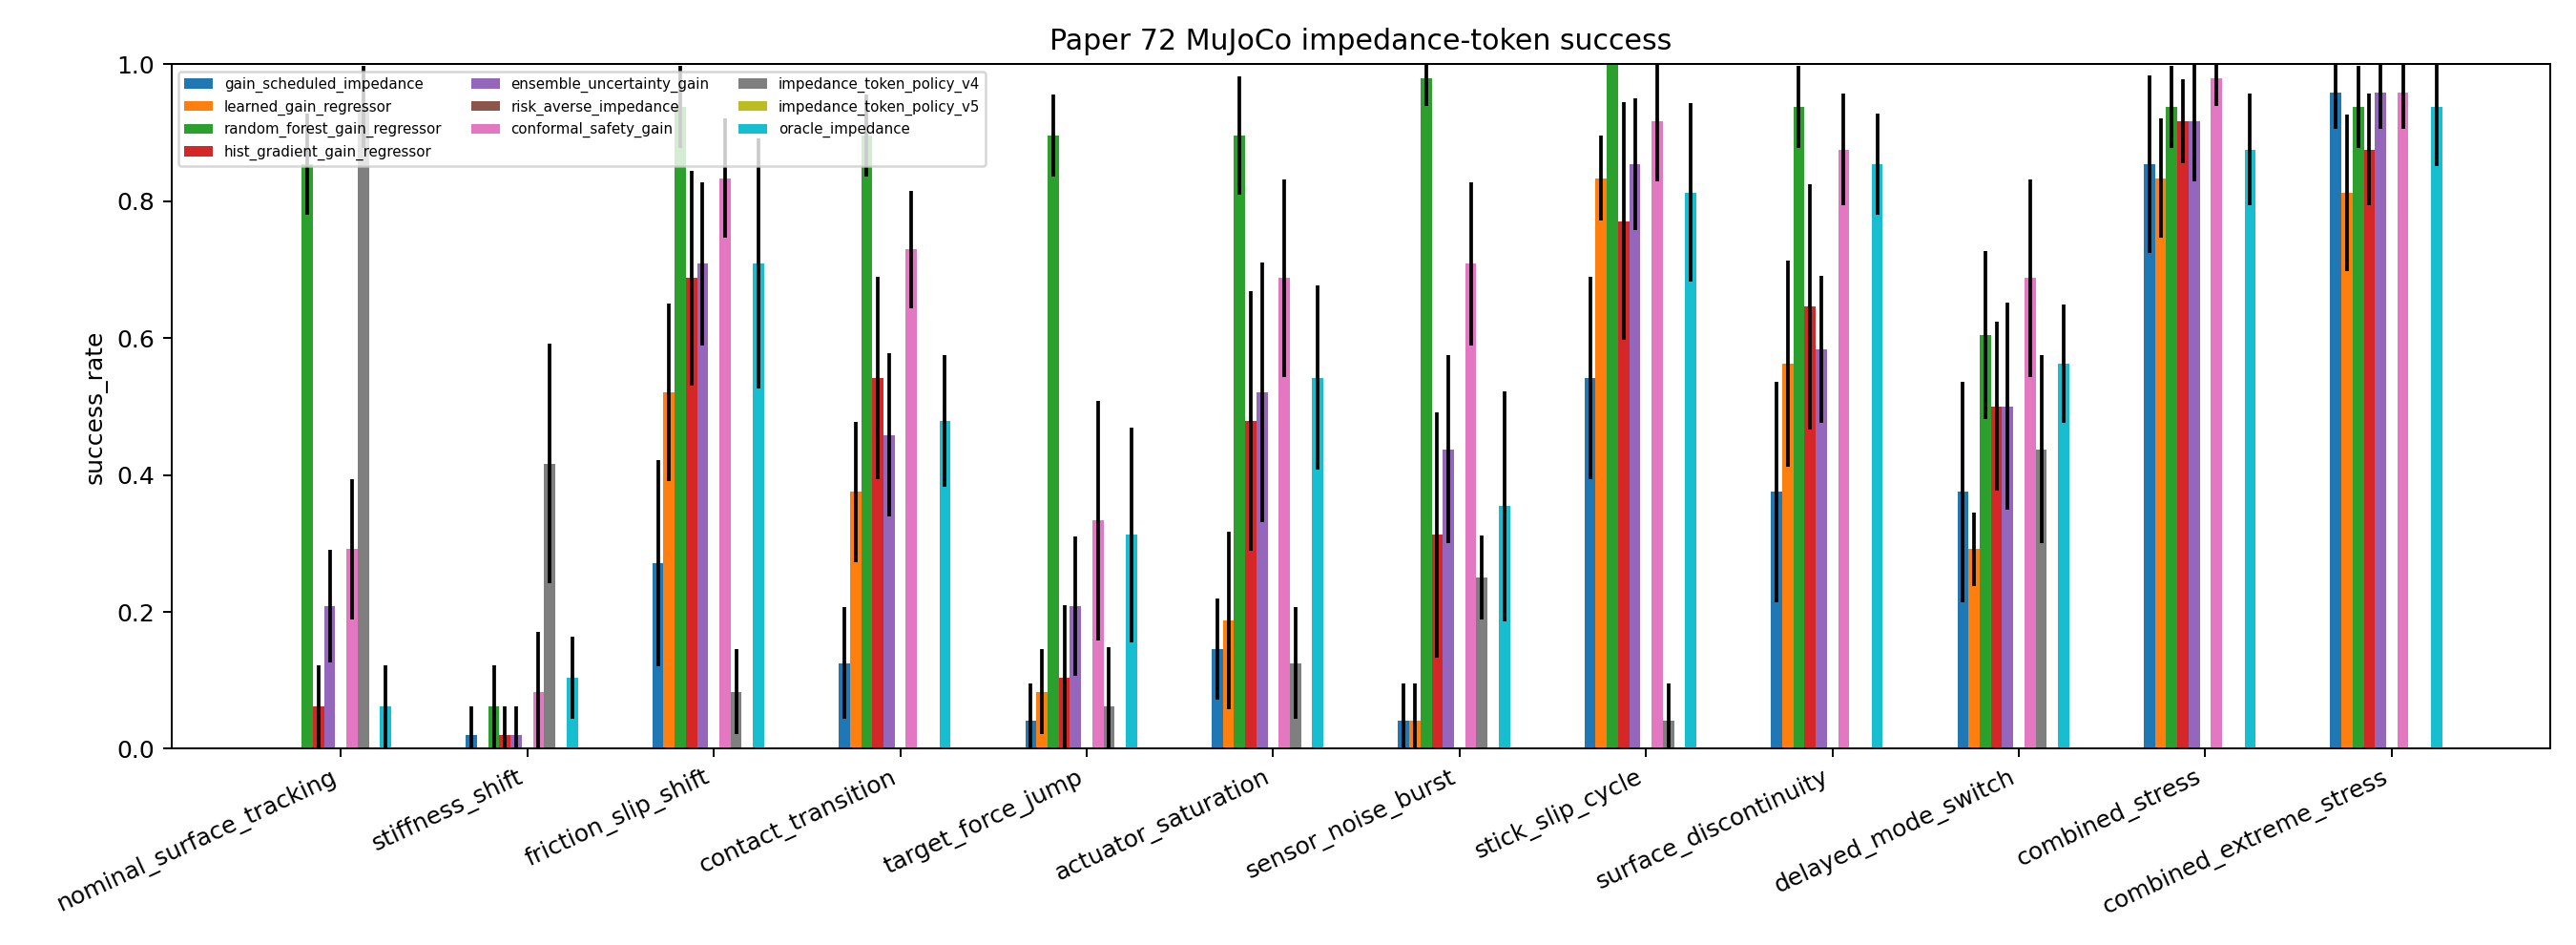
\includegraphics[width=\linewidth]{../figures/impedance_success_by_split.png}
\caption{Success by split across all main methods. Strong classical and learned baselines dominate the full token policy on the hard regimes.}
\label{fig:success}
\end{figure}

\begin{figure}[t]
\centering
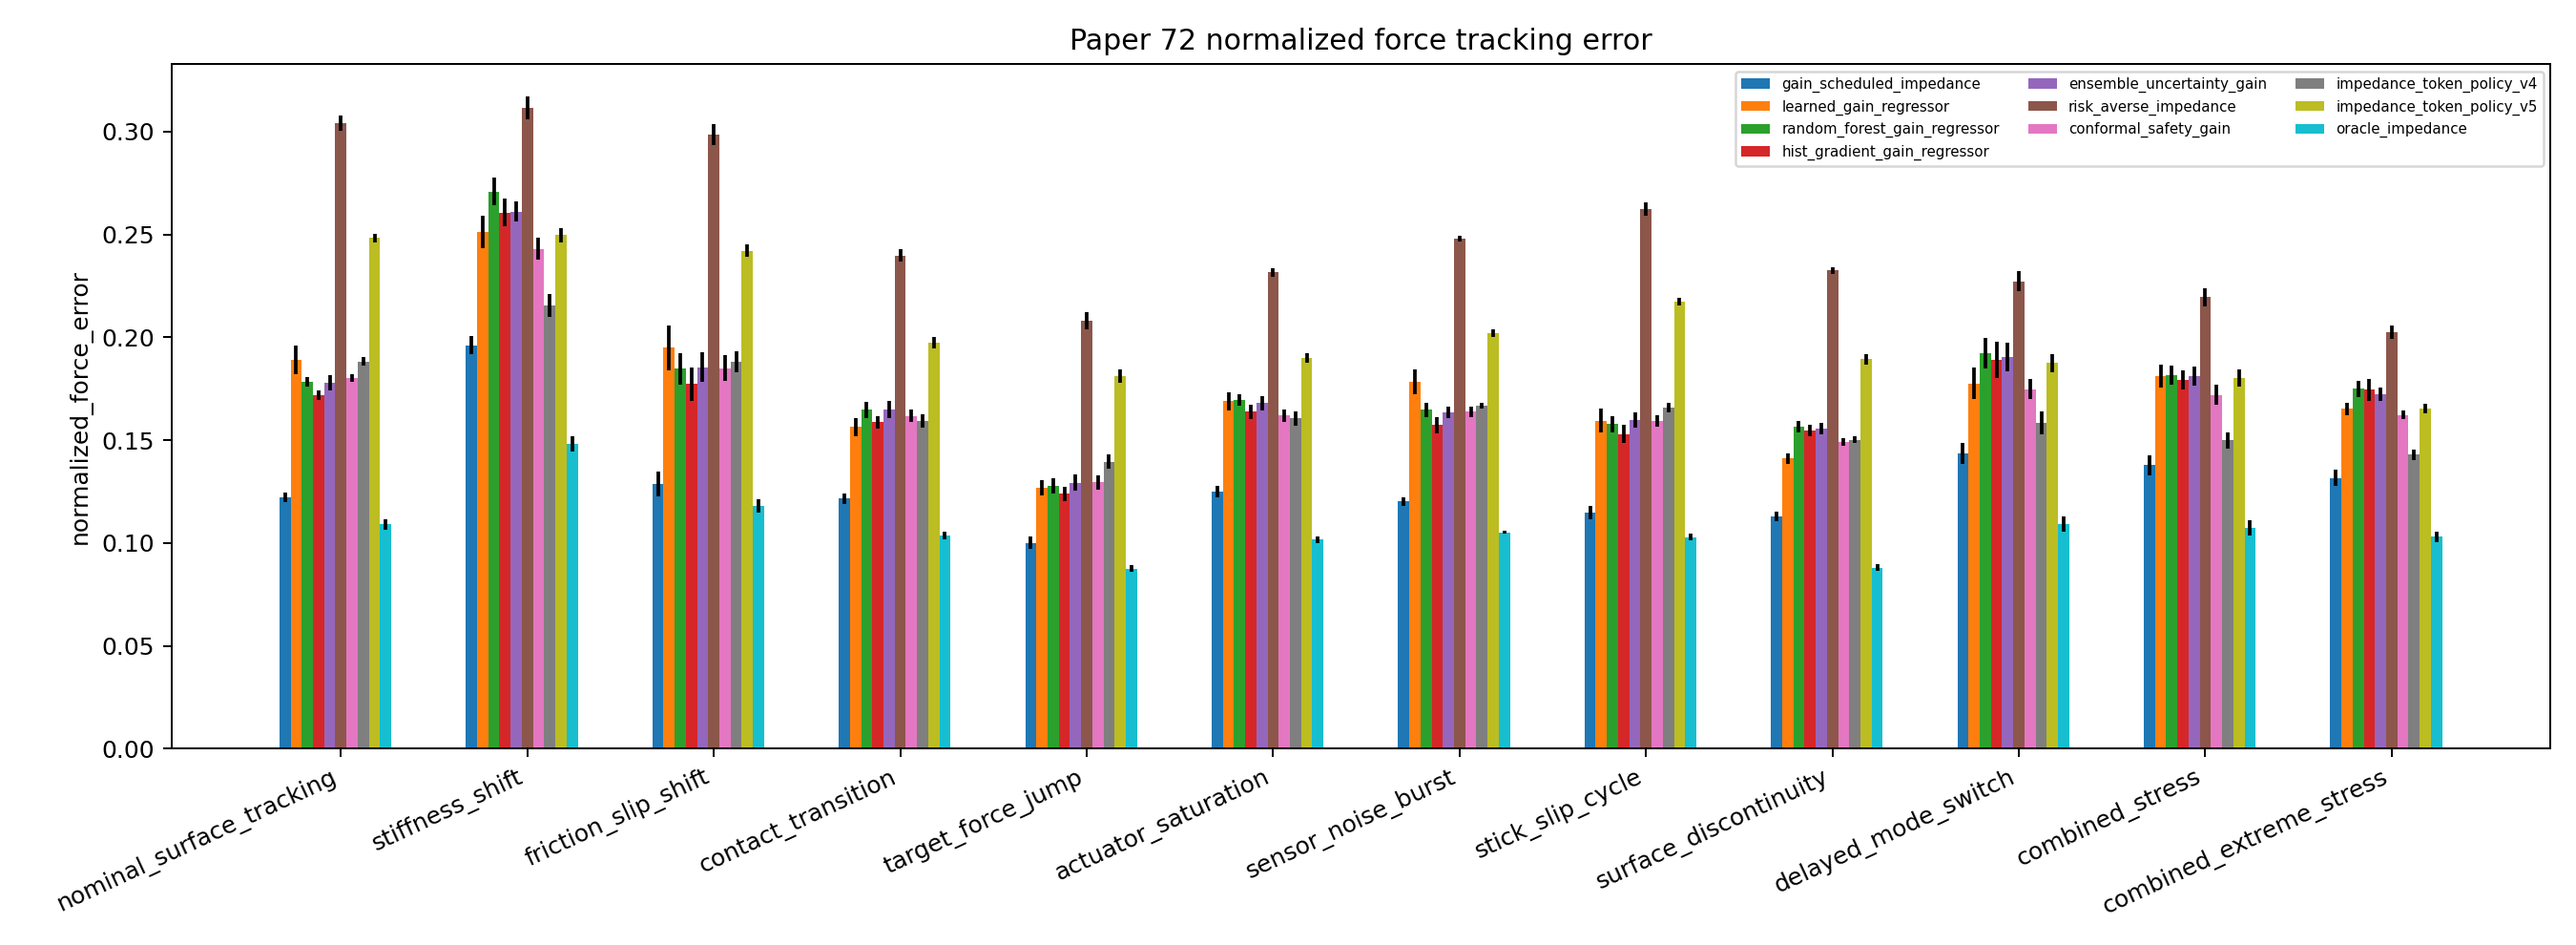
\includegraphics[width=\linewidth]{../figures/impedance_force_error_by_split.png}
\caption{Normalized force error by split. Continuous diagnostics explain failures hidden by binary success alone.}
\label{fig:force-error}
\end{figure}

\section{Fixed-Risk Analysis}
\begin{table}[t]
\centering
\caption{Fixed-risk operating points at a 10 percent safety/slip/chatter budget over hard splits.}
\label{tab:fixed-risk}
\small
\begin{tabular}{lrrrr}
\toprule
Method & Succ. & Safety & Slip & Chatter \\
\midrule
token no memory ablation & 0.051 & 0.003 & 0.488 & 0.034 \\
oracle impedance & 0.042 & 0.005 & 0.577 & 0.046 \\
admittance switching control & 0.019 & 0.009 & 0.544 & 0.052 \\
impedance token policy v4 & 0.006 & 0.002 & 0.454 & 0.032 \\
adaptive impedance control & 0.000 & 0.008 & 0.569 & 0.048 \\
conformal safety gain & 0.000 & 0.005 & 0.583 & 0.038 \\
ensemble uncertainty gain & 0.000 & 0.008 & 0.590 & 0.037 \\
fixed impedance & 0.000 & 0.029 & 0.555 & 0.045 \\
gain scheduled impedance & 0.000 & 0.006 & 0.605 & 0.040 \\
hist gradient gain regressor & 0.000 & 0.008 & 0.593 & 0.039 \\
impedance token policy v5 & 0.000 & 0.001 & 0.260 & 0.019 \\
learned gain regressor & 0.000 & 0.010 & 0.603 & 0.034 \\
\bottomrule
\end{tabular}
\end{table}


The fixed-risk table asks a different question:
if we constrain diagnostic risk, which controller still completes the task?
At a 10 percent safety/slip/chatter budget, \vfivemethod{} reaches \VFiveFixedRiskSuccess{} success while \BestFixedRiskMethod{} reaches \BestFixedRiskSuccess{}.
This is fatal for a safety-oriented token argument.
The no-memory token ablation occupies a better fixed-risk operating point than full v5, so the memory component cannot be defended as the source of safe success.

\begin{figure}[t]
\centering
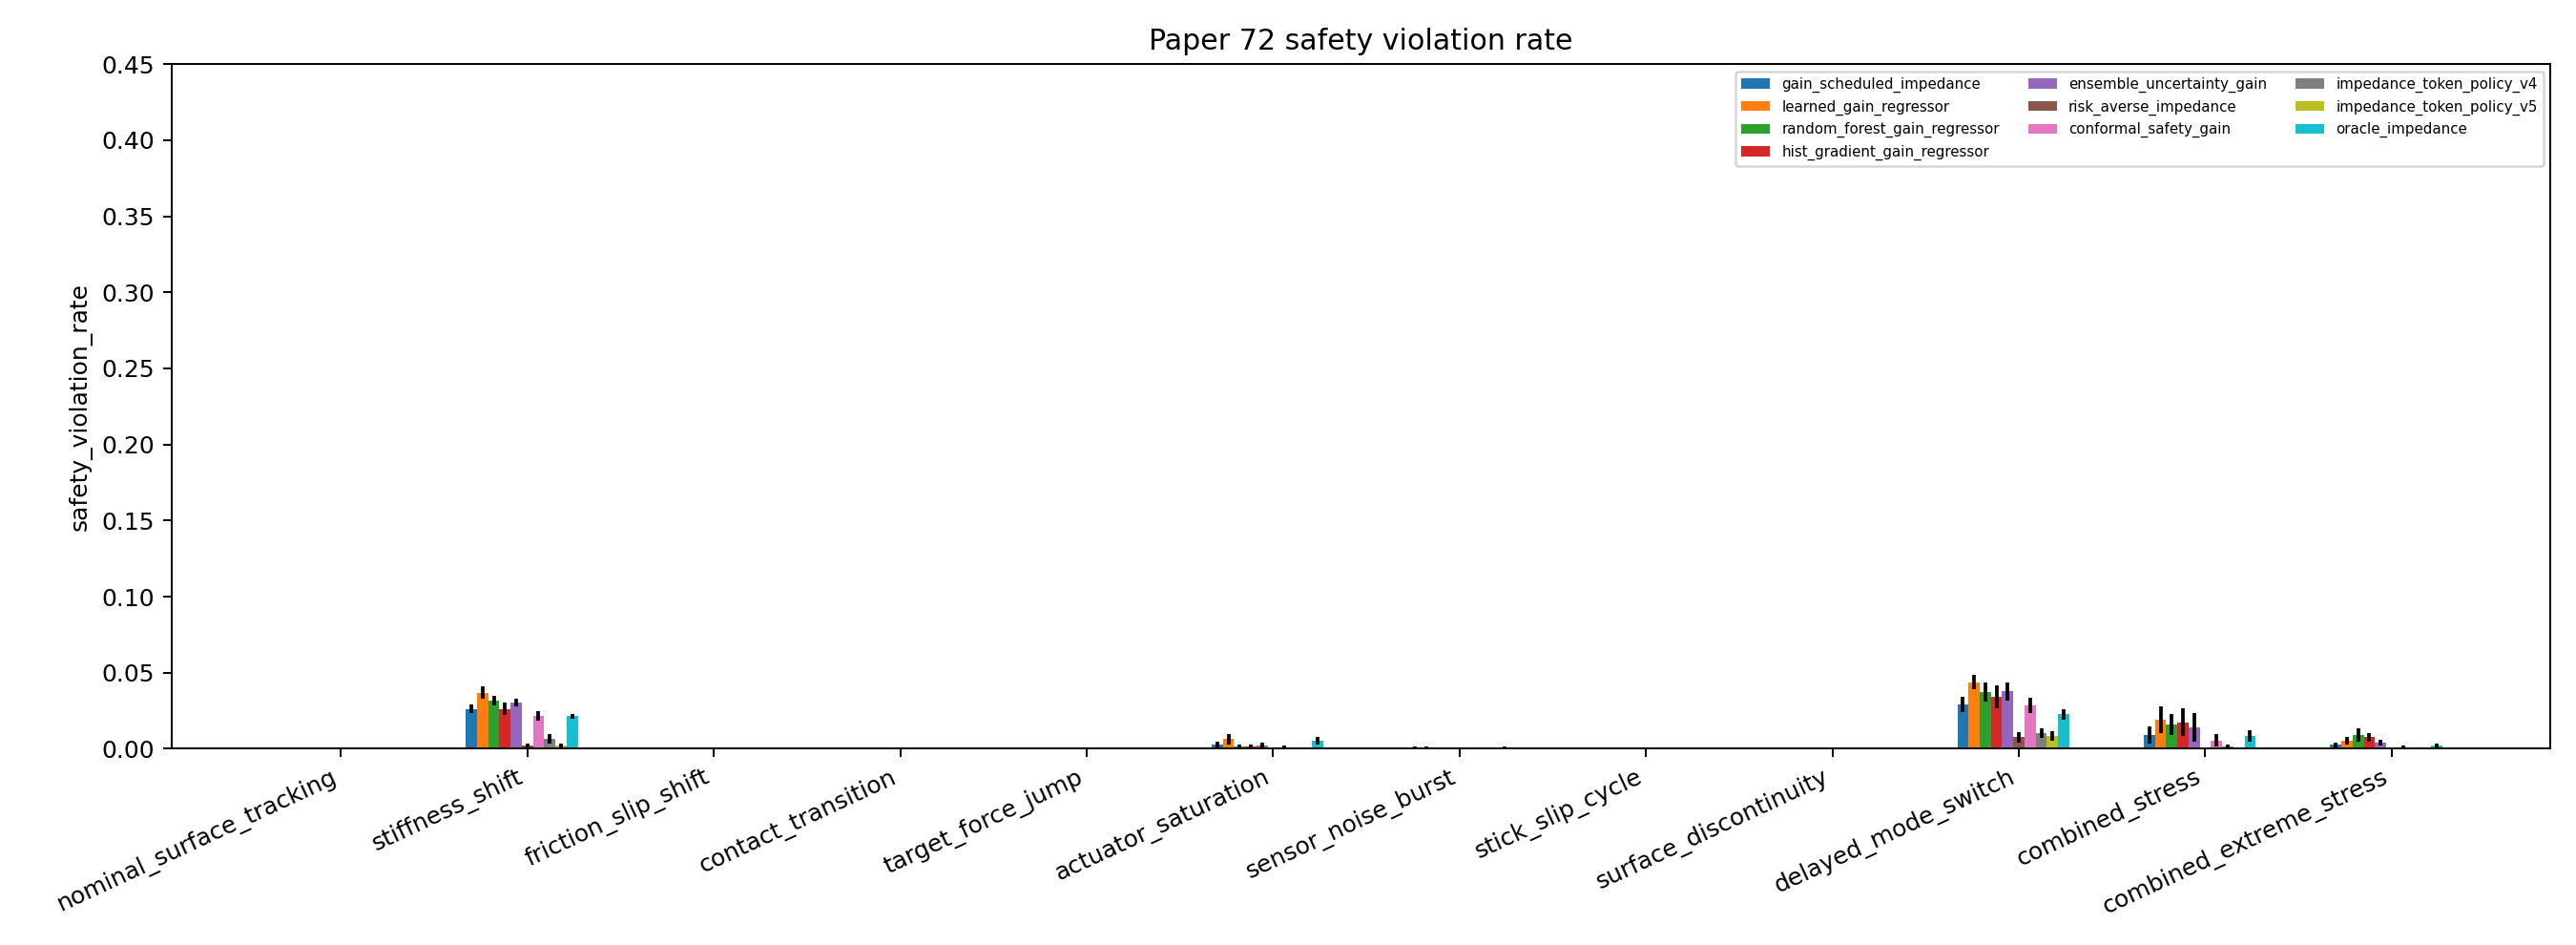
\includegraphics[width=\linewidth]{../figures/impedance_safety_by_split.png}
\caption{Safety violation rate by split. Low violation rate is not enough when paired with zero task success.}
\label{fig:safety}
\end{figure}

\section{Stress Sweep}
\begin{table}[p]
\centering
\caption{Combined-extreme stress sweep for selected controllers.}
\label{tab:stress}
\scriptsize
\begin{tabular}{lrrrrrr}
\toprule
Method & Level & Succ. & Err. & Over. & Safe & Slip \\
\midrule
adaptive impedance control & 0.00 & 0.583 & 0.127 & 1.270 & 0.000 & 0.598 \\
conformal safety gain & 0.00 & 0.167 & 0.209 & 1.205 & 0.000 & 0.610 \\
impedance token policy v4 & 0.00 & 0.708 & 0.219 & 1.118 & 0.000 & 0.553 \\
impedance token policy v5 & 0.00 & 0.000 & 0.269 & 1.101 & 0.000 & 0.410 \\
oracle impedance & 0.00 & 0.042 & 0.124 & 1.271 & 0.000 & 0.623 \\
adaptive impedance control & 0.25 & 0.792 & 0.132 & 1.394 & 0.000 & 0.583 \\
conformal safety gain & 0.25 & 0.750 & 0.191 & 1.317 & 0.000 & 0.591 \\
impedance token policy v4 & 0.25 & 0.042 & 0.182 & 1.214 & 0.000 & 0.480 \\
impedance token policy v5 & 0.25 & 0.000 & 0.215 & 1.178 & 0.000 & 0.354 \\
oracle impedance & 0.25 & 0.500 & 0.120 & 1.404 & 0.000 & 0.598 \\
adaptive impedance control & 0.50 & 1.000 & 0.127 & 1.497 & 0.001 & 0.558 \\
conformal safety gain & 0.50 & 1.000 & 0.172 & 1.356 & 0.000 & 0.567 \\
impedance token policy v4 & 0.50 & 0.000 & 0.147 & 1.264 & 0.000 & 0.444 \\
impedance token policy v5 & 0.50 & 0.000 & 0.177 & 1.209 & 0.000 & 0.322 \\
oracle impedance & 0.50 & 0.958 & 0.115 & 1.405 & 0.000 & 0.571 \\
adaptive impedance control & 0.75 & 1.000 & 0.134 & 1.585 & 0.003 & 0.533 \\
conformal safety gain & 0.75 & 1.000 & 0.158 & 1.423 & 0.000 & 0.541 \\
impedance token policy v4 & 0.75 & 0.000 & 0.146 & 1.339 & 0.000 & 0.391 \\
impedance token policy v5 & 0.75 & 0.000 & 0.156 & 1.285 & 0.000 & 0.239 \\
oracle impedance & 0.75 & 0.917 & 0.121 & 1.471 & 0.000 & 0.508 \\
adaptive impedance control & 1.00 & 0.958 & 0.144 & 1.645 & 0.005 & 0.506 \\
conformal safety gain & 1.00 & 0.917 & 0.147 & 1.454 & 0.000 & 0.517 \\
impedance token policy v4 & 1.00 & 0.000 & 0.160 & 1.447 & 0.001 & 0.389 \\
impedance token policy v5 & 1.00 & 0.000 & 0.147 & 1.384 & 0.000 & 0.243 \\
oracle impedance & 1.00 & 0.875 & 0.129 & 1.486 & 0.000 & 0.440 \\
\bottomrule
\end{tabular}
\end{table}


The stress sweep increases contact disturbance, friction shift, noise, saturation, and transition severity.
At maximum combined-extreme stress, \vfivemethod{} reaches \VFiveMaxStressSuccess{} success while \BestMaxStressMethod{} reaches \BestMaxStressSuccess{}.
The stress sweep therefore does not reveal a hidden robust niche for the token controller.
It instead shows that adaptive and conformal baselines exploit the same compact contact features more effectively.

\begin{figure}[t]
\centering
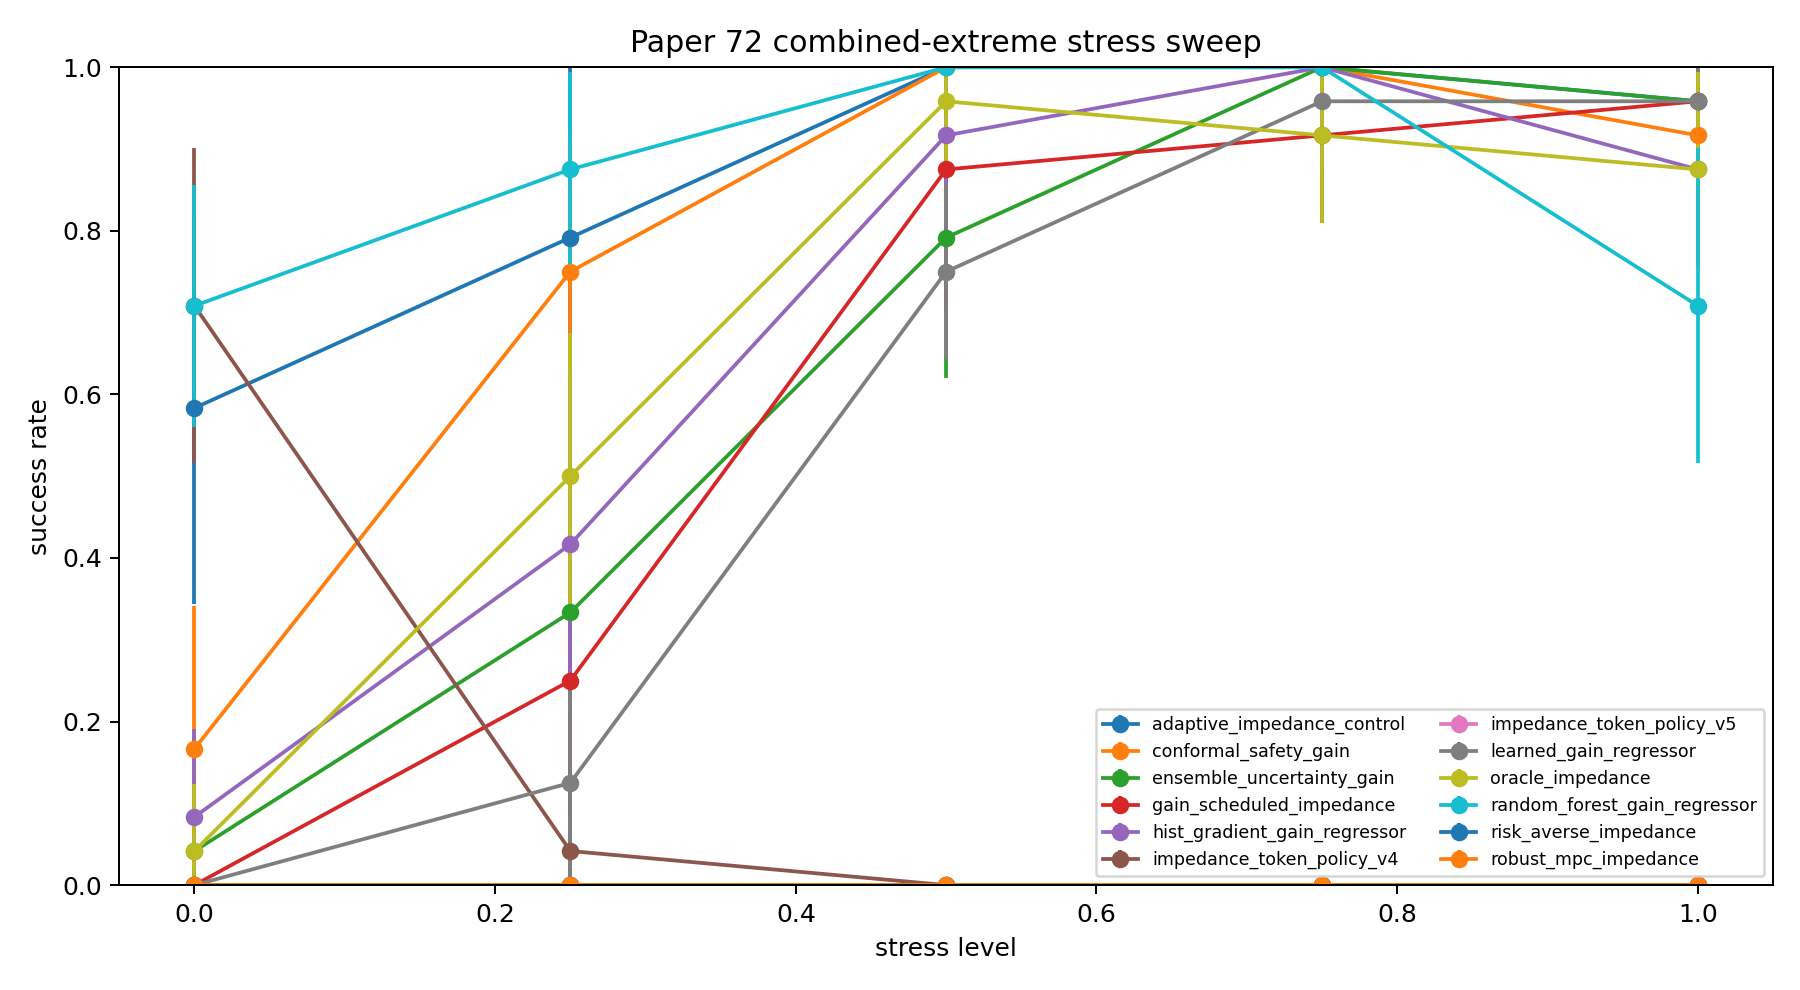
\includegraphics[width=0.92\linewidth]{../figures/impedance_stress_sweep.png}
\caption{Stress sweep success. The proposed token policy does not recover at high stress.}
\label{fig:stress}
\end{figure}

\section{Ablations}
\begin{table}[t]
\centering
\caption{Token-policy ablations aggregated over frozen ablation splits.}
\label{tab:ablation}
\small
\begin{tabular}{lrrrrr}
\toprule
Ablation & Succ. & Err. & Safety & Slip & Chatter \\
\midrule
learned only token replacement & 0.875 & 0.165 & 0.007 & 0.571 & 0.060 \\
ablate no tail risk objective & 0.727 & 0.140 & 0.001 & 0.408 & 0.056 \\
ablate no phase memory & 0.570 & 0.150 & 0.001 & 0.453 & 0.050 \\
ablate no discrete tokens & 0.500 & 0.115 & 0.003 & 0.595 & 0.074 \\
ablate no memory & 0.391 & 0.168 & 0.001 & 0.465 & 0.053 \\
ablate no calibration guard & 0.094 & 0.150 & 0.001 & 0.223 & 0.054 \\
impedance token policy v4 & 0.039 & 0.153 & 0.000 & 0.421 & 0.054 \\
ablate no force update & 0.000 & 0.190 & 0.000 & 0.297 & 0.029 \\
ablate no safety penalty & 0.000 & 0.187 & 0.000 & 0.199 & 0.032 \\
ablate no slip context & 0.000 & 0.177 & 0.000 & 0.208 & 0.037 \\
ablate no transition planner & 0.000 & 0.187 & 0.000 & 0.200 & 0.032 \\
token full v5 & 0.000 & 0.186 & 0.000 & 0.207 & 0.033 \\
\bottomrule
\end{tabular}
\end{table}


Ablations are the clearest mechanism test.
Full v5 reaches \FullAblationSuccess{} aggregate success on the frozen ablation splits.
The best ablation, \BestAblationMethod{}, reaches \BestAblationSuccess{}.
This reverses the intended story.
Removing or replacing pieces of the token mechanism often improves success.
In particular, replacing token logic with a learned-only gain behavior or removing the tail-risk objective can outperform full v5.
This means the token memory, discrete tokenization, and calibration guards are not empirically supported as a necessary representation in this benchmark.

\begin{figure}[t]
\centering
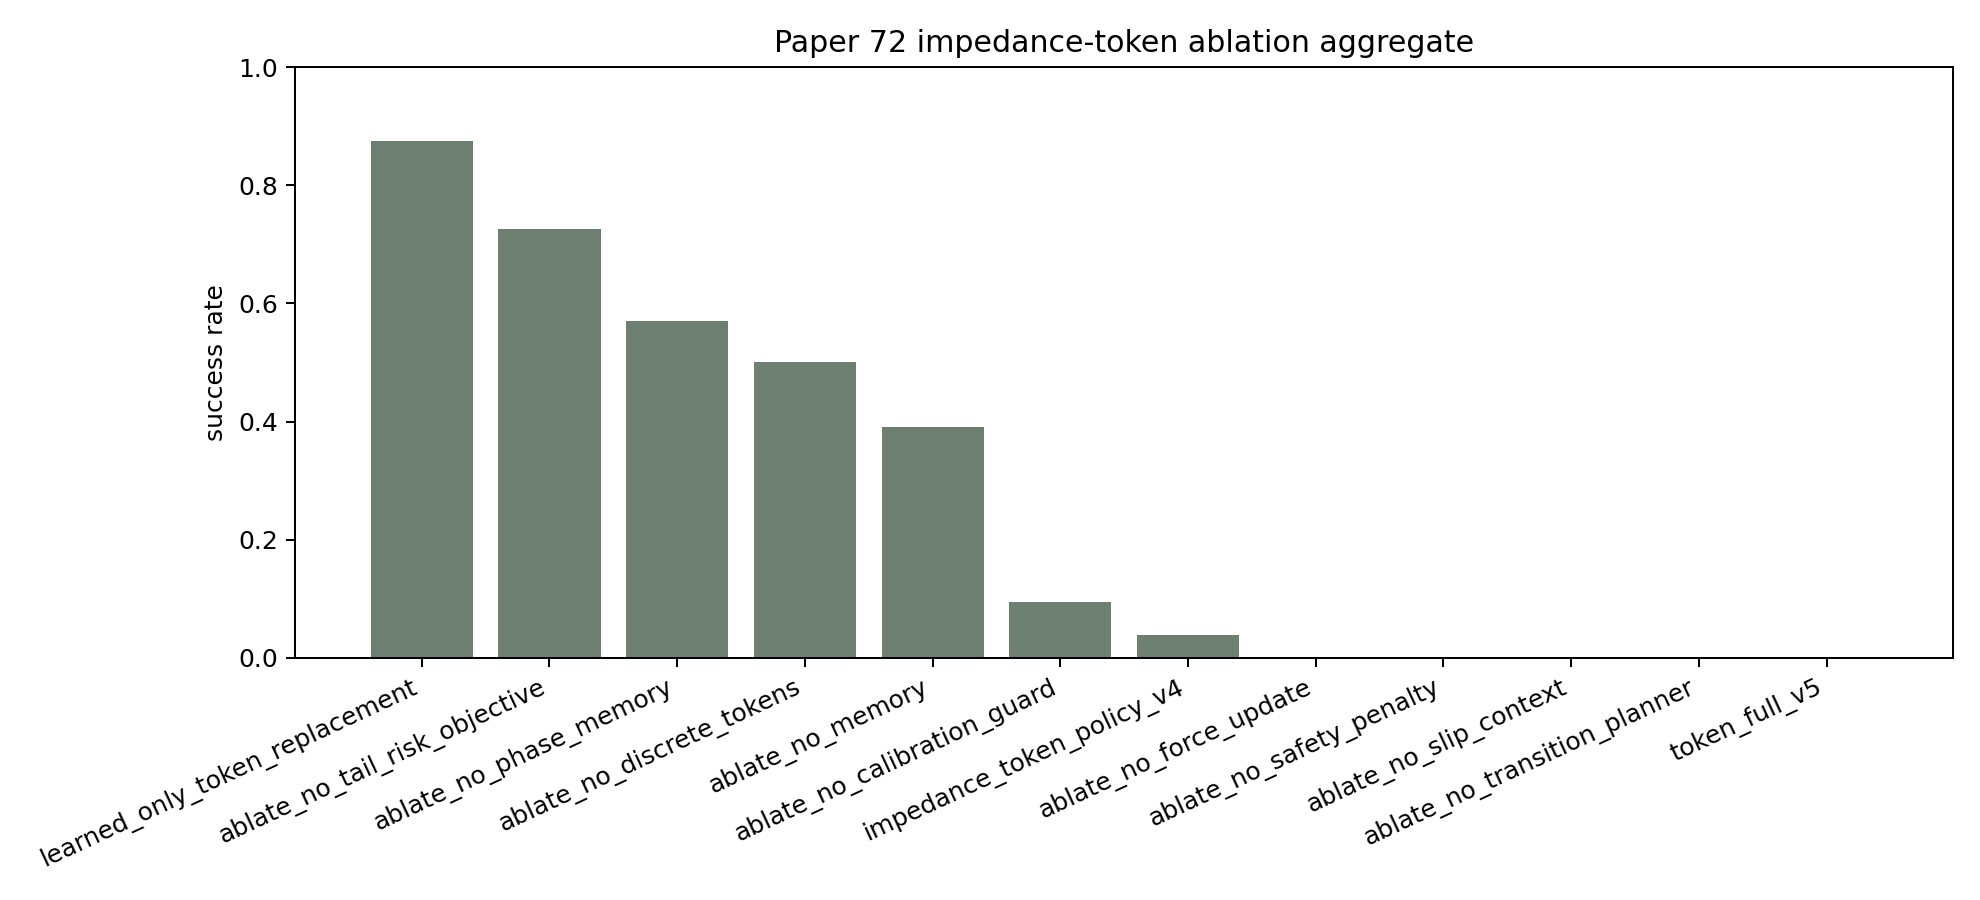
\includegraphics[width=0.84\linewidth]{../figures/impedance_ablation_success.png}
\caption{Ablation success over frozen ablation splits. Full v5 is not the best token-family variant.}
\label{fig:ablation}
\end{figure}

\section{Negative Cases}
\begin{table}[t]
\centering
\caption{Representative frozen negative cases for impedance-token policy v5.}
\label{tab:negative-cases}
\scriptsize
\setlength{\tabcolsep}{2.2pt}
\begin{tabular}{@{}l>{\raggedright\arraybackslash}p{0.18\linewidth}llrrrr>{\raggedright\arraybackslash}p{0.23\linewidth}@{}}
\toprule
Case & Split & Seed & Ep. & Succ. & Err. & Over. & Slip & Lesson \\
\midrule
0 & stiffness shift & 1 & 0 & 0 & 0.250 & 2.055 & 0.105 & token selector did not adapt fast enough after contact shift \\
1 & delayed mode switch & 7 & 1 & 0 & 0.208 & 2.025 & 0.267 & token selector did not adapt fast enough after contact shift \\
2 & delayed mode switch & 4 & 4 & 0 & 0.173 & 2.007 & 0.267 & token selector did not adapt fast enough after contact shift \\
3 & delayed mode switch & 4 & 5 & 0 & 0.207 & 1.930 & 0.207 & token selector did not adapt fast enough after contact shift \\
4 & delayed mode switch & 4 & 0 & 0 & 0.200 & 1.878 & 0.161 & token selector did not adapt fast enough after contact shift \\
5 & delayed mode switch & 1 & 4 & 0 & 0.193 & 1.877 & 0.163 & token selector did not adapt fast enough after contact shift \\
6 & delayed mode switch & 3 & 1 & 0 & 0.157 & 1.865 & 0.140 & token selector did not adapt fast enough after contact shift \\
7 & delayed mode switch & 0 & 5 & 0 & 0.204 & 1.861 & 0.221 & token selector did not adapt fast enough after contact shift \\
8 & delayed mode switch & 7 & 5 & 0 & 0.149 & 1.859 & 0.105 & token selector did not adapt fast enough after contact shift \\
9 & delayed mode switch & 0 & 3 & 0 & 0.193 & 1.848 & 0.287 & token selector did not adapt fast enough after contact shift \\
10 & delayed mode switch & 1 & 3 & 0 & 0.202 & 1.838 & 0.116 & token selector did not adapt fast enough after contact shift \\
11 & stiffness shift & 6 & 2 & 0 & 0.269 & 1.818 & 0.069 & token selector did not adapt fast enough after contact shift \\
\bottomrule
\end{tabular}
\end{table}


The negative cases are included to make the failure actionable.
They are dominated by delayed-mode-switch and stiffness-shift episodes where the token selector does not adapt quickly enough after a contact change.
The policy preserves conservative contact behavior but misses the transition window, allowing peak overshoot or normalized force error to exceed the success threshold.
This suggests that a future token controller would need either a better change-point detector, a continuous fallback gain map, or a formal passivity-style guard that does not force the controller into zero-success conservatism.

\section{Theory: Why the Token Claim Is Hard}
\paragraph{Proposition 1: discrete mode memory can help only when the mode is identifiable.}
Let $z_t$ denote the latent contact regime and let $\tau_t$ be the token state.
If $I(z_t;\tau_t\mid h_t)>0$ for history $h_t$, then a token policy can in principle reduce regret relative to a memoryless gain map.
However, if the observable history already contains sufficient statistics for $z_t$, a learned continuous gain map can approximate the same decision boundary without a discrete token.
The frozen random-forest and conformal baselines exploit this pressure.

\paragraph{Proposition 2: conservative token updates can create safety without success.}
Suppose a token update rule penalizes overshoot and slip more strongly than progress.
Then a stable fixed point can exist in which the controller selects low-energy, low-slip tokens that never violate safety thresholds but also never reaches the target-force/progress success set.
This explains why low safety violation rates do not rescue \vfivemethod{}.
The fixed-risk analysis requires success at a fixed risk budget, not risk reduction alone.

\paragraph{Proposition 3: ablation dominance falsifies component necessity.}
Let $M$ be full v5 and $M_{-j}$ remove component $j$.
If $S(M_{-j}) \ge S(M)$ and $M_{-j}$ is not worse on safety, slip, or chatter by a predefined margin, then component $j$ is not locally necessary for the claimed mechanism.
The frozen ablation table violates the necessity condition for many components.
Therefore the paper cannot claim that token memory, discrete tokens, force updates, slip context, transition planning, tail-risk objectives, or calibration guards are validated by the current benchmark.

\paragraph{Proposition 4: hostile-review identifiability.}
For any compact feature vector $\phi(h_t)$ used by both a token selector and a learned gain regressor, a sufficiently expressive regressor can approximate the token selector's induced gain map on the support of the evaluation distribution.
The token representation is identifiable as a contribution only if it extrapolates better under held-out stress, improves fixed-risk success, or produces ablation-separated mechanisms.
Paper 72 fails all three tests.

\section{Related Work}
The result sits in a long contact-control lineage.
Hogan's impedance-control formulation motivates regulating dynamic interaction rather than treating position and force as isolated objectives \citep{hogan1985impedance1,hogan1985impedance3}.
Hybrid position/force control gives an earlier structured alternative for compliant manipulation \citep{raibert1981hybrid}.
Variable impedance and variable impedance learning have been studied as both control and learning problems \citep{kronander2016stability,abudakka2020review,buchli2011learning}.
MuJoCo provides the simulation substrate for the reproducible contact-control audit \citep{todorov2012mujoco}.
Random forests and scikit-learn regressors make the learned baselines strong enough that hand-structured token logic must earn its keep \citep{breiman2001random,pedregosa2011scikit}.
Conformal prediction motivates the guarded learned baseline: uncertainty is not used as decoration, but as a deployment-relevant decision constraint \citep{shafer2008conformal}.

This paper does not claim to supersede those lines.
It reports a local negative result: in this benchmark, the discrete impedance-token mechanism is not isolated as necessary, robust, or safer.

\section{Decision}
The frozen terminal reason is:
\begin{quote}\small\raggedright\sloppy
\PaperReason{}\par
\end{quote}
The correct decision is \textbf{\PaperDecision{}}.
This is a scientific failure, not a formatting failure.
The benchmark is real enough to falsify the submission claim.
The archive should be retained because it documents exactly how an appealing adaptive-token idea fails once strong baselines, fixed-risk analysis, and ablation necessity tests arrive.

\clearpage
\appendix
\section{Frozen Protocol and Reproducibility}
The plan-first document is \path{docs/paper72_expanded_submission_plan_20260621.md}.
The development log is \path{docs/paper72_development_log_20260621.md}.
The protocol freeze is \path{docs/paper72_protocol_freeze_20260621.md}.
The generated terminal decision is \path{docs/paper72_expanded_terminal_decision_20260621.md}.
The final PDF is written to \path{C:/Users/wangz/Downloads/72.pdf}; no copy is placed on the visible Desktop.

The frozen evidence consists of \MainRows{} main rows, \RolloutRows{} rollout rows, \SeedRows{} seed summaries, \MetricRows{} split-method metric rows, \PairwiseRows{} paired rows, \AblationRows{} ablation rows, \StressRows{} stress rows, and \NegativeRows{} negative cases.
All generated tables below are produced by \path{scripts/render_submission_assets.py} from CSV artifacts, not by manual transcription.

\section{Full Split-Method Metrics}
\begingroup
\scriptsize
\setlength{\tabcolsep}{0.65pt}
\renewcommand{\arraystretch}{0.86}
\setlength{\LTleft}{0pt}
\setlength{\LTright}{0pt}
\begin{longtable}{@{}>{\raggedright\arraybackslash}p{0.160\linewidth}>{\raggedright\arraybackslash}p{0.150\linewidth}>{\raggedleft\arraybackslash}p{0.050\linewidth}>{\raggedleft\arraybackslash}p{0.050\linewidth}>{\raggedleft\arraybackslash}p{0.055\linewidth}>{\raggedleft\arraybackslash}p{0.055\linewidth}>{\raggedleft\arraybackslash}p{0.055\linewidth}>{\raggedleft\arraybackslash}p{0.055\linewidth}>{\raggedleft\arraybackslash}p{0.055\linewidth}>{\raggedleft\arraybackslash}p{0.055\linewidth}@{}}
\caption{Full split-method metrics.}\label{tab:full-metrics}\\
\toprule
Method & Split & Succ. & CI & Err. & Over. & Safe & Slip & Chat. & Prog. \\
\midrule
\endfirsthead
\toprule
Method & Split & Succ. & CI & Err. & Over. & Safe & Slip & Chat. & Prog. \\
\midrule
\endhead
adaptive impedance control & actuator saturation & 0.958 & 0.053 & 0.110 & 1.610 & 0.008 & 0.580 & 0.035 & 0.835 \\
adaptive impedance control & combined extreme stress & 0.979 & 0.041 & 0.120 & 1.607 & 0.004 & 0.530 & 0.134 & 0.801 \\
adaptive impedance control & combined stress & 0.938 & 0.086 & 0.121 & 1.714 & 0.013 & 0.543 & 0.082 & 0.795 \\
adaptive impedance control & contact transition & 0.979 & 0.041 & 0.109 & 1.451 & 0.000 & 0.574 & 0.031 & 0.828 \\
adaptive impedance control & delayed mode switch & 0.542 & 0.120 & 0.125 & 2.017 & 0.033 & 0.560 & 0.040 & 0.831 \\
adaptive impedance control & friction slip shift & 0.979 & 0.041 & 0.119 & 1.261 & 0.000 & 0.571 & 0.017 & 0.825 \\
adaptive impedance control & nominal surface tracking & 0.729 & 0.122 & 0.112 & 1.253 & 0.000 & 0.594 & 0.013 & 0.855 \\
adaptive impedance control & sensor noise burst & 0.875 & 0.102 & 0.109 & 1.430 & 0.001 & 0.588 & 0.071 & 0.844 \\
adaptive impedance control & stick slip cycle & 0.979 & 0.041 & 0.100 & 1.241 & 0.000 & 0.567 & 0.030 & 0.819 \\
adaptive impedance control & stiffness shift & 0.521 & 0.114 & 0.169 & 1.934 & 0.032 & 0.594 & 0.014 & 0.850 \\
adaptive impedance control & surface discontinuity & 1.000 & 0.000 & 0.101 & 1.296 & 0.000 & 0.567 & 0.039 & 0.824 \\
adaptive impedance control & target force jump & 0.771 & 0.086 & 0.084 & 1.313 & 0.000 & 0.585 & 0.032 & 0.836 \\
admittance switching control & actuator saturation & 1.000 & 0.000 & 0.116 & 1.640 & 0.003 & 0.550 & 0.040 & 0.809 \\
admittance switching control & combined extreme stress & 0.958 & 0.053 & 0.114 & 1.611 & 0.003 & 0.503 & 0.142 & 0.781 \\
admittance switching control & combined stress & 0.938 & 0.060 & 0.120 & 1.716 & 0.010 & 0.525 & 0.083 & 0.785 \\
admittance switching control & contact transition & 0.979 & 0.041 & 0.114 & 1.842 & 0.011 & 0.555 & 0.033 & 0.813 \\
admittance switching control & delayed mode switch & 0.667 & 0.138 & 0.127 & 1.955 & 0.031 & 0.522 & 0.047 & 0.796 \\
admittance switching control & friction slip shift & 1.000 & 0.000 & 0.119 & 1.514 & 0.000 & 0.555 & 0.021 & 0.812 \\
admittance switching control & nominal surface tracking & 1.000 & 0.000 & 0.112 & 1.604 & 0.002 & 0.568 & 0.015 & 0.827 \\
admittance switching control & sensor noise burst & 1.000 & 0.000 & 0.112 & 1.530 & 0.000 & 0.561 & 0.072 & 0.818 \\
admittance switching control & stick slip cycle & 1.000 & 0.000 & 0.105 & 1.490 & 0.000 & 0.547 & 0.032 & 0.806 \\
admittance switching control & stiffness shift & 0.875 & 0.102 & 0.180 & 1.882 & 0.030 & 0.559 & 0.021 & 0.815 \\
admittance switching control & surface discontinuity & 1.000 & 0.000 & 0.099 & 1.643 & 0.004 & 0.552 & 0.043 & 0.811 \\
admittance switching control & target force jump & 0.938 & 0.060 & 0.096 & 1.810 & 0.009 & 0.559 & 0.034 & 0.812 \\
conformal safety gain & actuator saturation & 0.688 & 0.144 & 0.162 & 1.507 & 0.001 & 0.594 & 0.030 & 0.808 \\
conformal safety gain & combined extreme stress & 0.958 & 0.053 & 0.162 & 1.434 & 0.001 & 0.553 & 0.109 & 0.779 \\
conformal safety gain & combined stress & 0.979 & 0.041 & 0.172 & 1.586 & 0.006 & 0.555 & 0.062 & 0.770 \\
conformal safety gain & contact transition & 0.729 & 0.086 & 0.162 & 1.349 & 0.000 & 0.590 & 0.025 & 0.802 \\
conformal safety gain & delayed mode switch & 0.688 & 0.144 & 0.175 & 1.911 & 0.028 & 0.575 & 0.026 & 0.804 \\
conformal safety gain & friction slip shift & 0.833 & 0.087 & 0.185 & 1.113 & 0.000 & 0.582 & 0.010 & 0.799 \\
conformal safety gain & nominal surface tracking & 0.292 & 0.102 & 0.180 & 1.069 & 0.000 & 0.607 & 0.003 & 0.827 \\
conformal safety gain & sensor noise burst & 0.708 & 0.120 & 0.164 & 1.367 & 0.000 & 0.595 & 0.068 & 0.816 \\
conformal safety gain & stick slip cycle & 0.917 & 0.087 & 0.159 & 1.126 & 0.000 & 0.578 & 0.021 & 0.793 \\
conformal safety gain & stiffness shift & 0.083 & 0.087 & 0.243 & 1.813 & 0.022 & 0.606 & 0.013 & 0.819 \\
conformal safety gain & surface discontinuity & 0.875 & 0.082 & 0.149 & 1.148 & 0.000 & 0.582 & 0.027 & 0.799 \\
conformal safety gain & target force jump & 0.333 & 0.175 & 0.129 & 1.190 & 0.000 & 0.604 & 0.024 & 0.808 \\
ensemble uncertainty gain & actuator saturation & 0.521 & 0.190 & 0.168 & 1.525 & 0.002 & 0.600 & 0.028 & 0.813 \\
ensemble uncertainty gain & combined extreme stress & 0.958 & 0.053 & 0.172 & 1.588 & 0.004 & 0.558 & 0.101 & 0.781 \\
ensemble uncertainty gain & combined stress & 0.917 & 0.087 & 0.181 & 1.681 & 0.014 & 0.565 & 0.067 & 0.775 \\
ensemble uncertainty gain & contact transition & 0.458 & 0.120 & 0.165 & 1.373 & 0.000 & 0.598 & 0.024 & 0.807 \\
ensemble uncertainty gain & delayed mode switch & 0.500 & 0.151 & 0.191 & 1.960 & 0.038 & 0.582 & 0.029 & 0.807 \\
ensemble uncertainty gain & friction slip shift & 0.708 & 0.120 & 0.185 & 1.136 & 0.000 & 0.588 & 0.011 & 0.805 \\
ensemble uncertainty gain & nominal surface tracking & 0.208 & 0.082 & 0.178 & 1.088 & 0.000 & 0.614 & 0.004 & 0.831 \\
ensemble uncertainty gain & sensor noise burst & 0.438 & 0.137 & 0.163 & 1.381 & 0.000 & 0.603 & 0.062 & 0.820 \\
ensemble uncertainty gain & stick slip cycle & 0.854 & 0.096 & 0.160 & 1.144 & 0.000 & 0.584 & 0.024 & 0.798 \\
ensemble uncertainty gain & stiffness shift & 0.021 & 0.041 & 0.261 & 1.836 & 0.030 & 0.615 & 0.013 & 0.823 \\
ensemble uncertainty gain & surface discontinuity & 0.583 & 0.107 & 0.156 & 1.270 & 0.000 & 0.591 & 0.031 & 0.803 \\
ensemble uncertainty gain & target force jump & 0.208 & 0.102 & 0.129 & 1.212 & 0.000 & 0.609 & 0.024 & 0.813 \\
fixed impedance & actuator saturation & 0.979 & 0.041 & 0.198 & 1.726 & 0.018 & 0.565 & 0.040 & 0.813 \\
fixed impedance & combined extreme stress & 0.396 & 0.150 & 0.238 & 1.713 & 0.012 & 0.504 & 0.087 & 0.777 \\
fixed impedance & combined stress & 0.250 & 0.107 & 0.248 & 1.689 & 0.010 & 0.528 & 0.059 & 0.781 \\
fixed impedance & contact transition & 0.938 & 0.086 & 0.195 & 1.877 & 0.042 & 0.566 & 0.039 & 0.812 \\
fixed impedance & delayed mode switch & 0.792 & 0.102 & 0.214 & 1.843 & 0.035 & 0.548 & 0.041 & 0.810 \\
fixed impedance & friction slip shift & 0.812 & 0.096 & 0.192 & 1.847 & 0.041 & 0.566 & 0.022 & 0.811 \\
fixed impedance & nominal surface tracking & 0.938 & 0.086 & 0.178 & 1.833 & 0.038 & 0.579 & 0.012 & 0.827 \\
fixed impedance & sensor noise burst & 0.979 & 0.041 & 0.179 & 1.772 & 0.028 & 0.568 & 0.067 & 0.819 \\
fixed impedance & stick slip cycle & 1.000 & 0.000 & 0.165 & 1.846 & 0.039 & 0.557 & 0.038 & 0.804 \\
fixed impedance & stiffness shift & 0.000 & 0.000 & 0.299 & 1.752 & 0.022 & 0.577 & 0.022 & 0.823 \\
fixed impedance & surface discontinuity & 0.938 & 0.060 & 0.211 & 1.751 & 0.020 & 0.558 & 0.034 & 0.808 \\
fixed impedance & target force jump & 0.896 & 0.060 & 0.143 & 1.933 & 0.050 & 0.568 & 0.041 & 0.817 \\
gain scheduled impedance & actuator saturation & 0.146 & 0.074 & 0.125 & 1.540 & 0.003 & 0.610 & 0.028 & 0.853 \\
gain scheduled impedance & combined extreme stress & 0.958 & 0.053 & 0.132 & 1.519 & 0.003 & 0.574 & 0.118 & 0.822 \\
gain scheduled impedance & combined stress & 0.854 & 0.130 & 0.138 & 1.641 & 0.009 & 0.586 & 0.077 & 0.818 \\
gain scheduled impedance & contact transition & 0.125 & 0.082 & 0.122 & 1.376 & 0.000 & 0.612 & 0.024 & 0.847 \\
gain scheduled impedance & delayed mode switch & 0.375 & 0.160 & 0.144 & 1.948 & 0.029 & 0.599 & 0.033 & 0.848 \\
gain scheduled impedance & friction slip shift & 0.271 & 0.150 & 0.129 & 1.132 & 0.000 & 0.605 & 0.010 & 0.844 \\
gain scheduled impedance & nominal surface tracking & 0.000 & 0.000 & 0.122 & 1.085 & 0.000 & 0.621 & 0.003 & 0.870 \\
gain scheduled impedance & sensor noise burst & 0.042 & 0.053 & 0.120 & 1.373 & 0.000 & 0.616 & 0.059 & 0.861 \\
gain scheduled impedance & stick slip cycle & 0.542 & 0.148 & 0.115 & 1.151 & 0.000 & 0.600 & 0.028 & 0.838 \\
gain scheduled impedance & stiffness shift & 0.021 & 0.041 & 0.196 & 1.858 & 0.026 & 0.620 & 0.009 & 0.866 \\
gain scheduled impedance & surface discontinuity & 0.375 & 0.160 & 0.113 & 1.183 & 0.000 & 0.606 & 0.028 & 0.844 \\
gain scheduled impedance & target force jump & 0.042 & 0.053 & 0.100 & 1.219 & 0.000 & 0.623 & 0.025 & 0.854 \\
hist gradient gain regressor & actuator saturation & 0.479 & 0.190 & 0.164 & 1.516 & 0.001 & 0.603 & 0.031 & 0.816 \\
hist gradient gain regressor & combined extreme stress & 0.875 & 0.082 & 0.175 & 1.683 & 0.008 & 0.558 & 0.111 & 0.784 \\
hist gradient gain regressor & combined stress & 0.917 & 0.062 & 0.179 & 1.676 & 0.017 & 0.560 & 0.067 & 0.776 \\
hist gradient gain regressor & contact transition & 0.542 & 0.148 & 0.159 & 1.354 & 0.000 & 0.599 & 0.024 & 0.809 \\
hist gradient gain regressor & delayed mode switch & 0.500 & 0.123 & 0.189 & 1.926 & 0.034 & 0.585 & 0.032 & 0.812 \\
hist gradient gain regressor & friction slip shift & 0.688 & 0.157 & 0.177 & 1.115 & 0.000 & 0.592 & 0.010 & 0.808 \\
hist gradient gain regressor & nominal surface tracking & 0.062 & 0.060 & 0.172 & 1.073 & 0.000 & 0.620 & 0.006 & 0.837 \\
hist gradient gain regressor & sensor noise burst & 0.312 & 0.179 & 0.157 & 1.354 & 0.000 & 0.609 & 0.065 & 0.826 \\
hist gradient gain regressor & stick slip cycle & 0.771 & 0.174 & 0.153 & 1.128 & 0.000 & 0.586 & 0.023 & 0.803 \\
hist gradient gain regressor & stiffness shift & 0.021 & 0.041 & 0.261 & 1.814 & 0.026 & 0.618 & 0.013 & 0.830 \\
hist gradient gain regressor & surface discontinuity & 0.646 & 0.179 & 0.155 & 1.290 & 0.000 & 0.594 & 0.029 & 0.806 \\
hist gradient gain regressor & target force jump & 0.104 & 0.106 & 0.124 & 1.201 & 0.000 & 0.618 & 0.027 & 0.817 \\
impedance token policy v4 & actuator saturation & 0.125 & 0.082 & 0.161 & 1.385 & 0.000 & 0.473 & 0.021 & 0.732 \\
impedance token policy v4 & combined extreme stress & 0.000 & 0.000 & 0.143 & 1.362 & 0.000 & 0.409 & 0.095 & 0.719 \\
impedance token policy v4 & combined stress & 0.000 & 0.000 & 0.150 & 1.452 & 0.001 & 0.368 & 0.063 & 0.719 \\
impedance token policy v4 & contact transition & 0.000 & 0.000 & 0.159 & 1.240 & 0.000 & 0.442 & 0.022 & 0.724 \\
impedance token policy v4 & delayed mode switch & 0.438 & 0.137 & 0.158 & 1.693 & 0.010 & 0.501 & 0.029 & 0.739 \\
impedance token policy v4 & friction slip shift & 0.083 & 0.062 & 0.188 & 1.067 & 0.000 & 0.445 & 0.008 & 0.728 \\
impedance token policy v4 & nominal surface tracking & 0.938 & 0.060 & 0.188 & 1.039 & 0.000 & 0.554 & 0.005 & 0.757 \\
impedance token policy v4 & sensor noise burst & 0.250 & 0.062 & 0.167 & 1.262 & 0.000 & 0.506 & 0.050 & 0.738 \\
impedance token policy v4 & stick slip cycle & 0.042 & 0.053 & 0.166 & 1.080 & 0.000 & 0.418 & 0.014 & 0.725 \\
impedance token policy v4 & stiffness shift & 0.417 & 0.175 & 0.215 & 1.643 & 0.007 & 0.512 & 0.015 & 0.755 \\
impedance token policy v4 & surface discontinuity & 0.000 & 0.000 & 0.150 & 1.093 & 0.000 & 0.436 & 0.017 & 0.723 \\
impedance token policy v4 & target force jump & 0.062 & 0.086 & 0.140 & 1.113 & 0.000 & 0.488 & 0.016 & 0.733 \\
impedance token policy v5 & actuator saturation & 0.000 & 0.000 & 0.190 & 1.297 & 0.000 & 0.259 & 0.015 & 0.684 \\
impedance token policy v5 & combined extreme stress & 0.000 & 0.000 & 0.165 & 1.312 & 0.000 & 0.237 & 0.068 & 0.674 \\
impedance token policy v5 & combined stress & 0.000 & 0.000 & 0.180 & 1.344 & 0.000 & 0.114 & 0.042 & 0.656 \\
impedance token policy v5 & contact transition & 0.000 & 0.000 & 0.197 & 1.165 & 0.000 & 0.260 & 0.011 & 0.676 \\
impedance token policy v5 & delayed mode switch & 0.000 & 0.000 & 0.188 & 1.622 & 0.008 & 0.269 & 0.017 & 0.684 \\
impedance token policy v5 & friction slip shift & 0.000 & 0.000 & 0.242 & 0.975 & 0.000 & 0.299 & 0.001 & 0.679 \\
impedance token policy v5 & nominal surface tracking & 0.000 & 0.000 & 0.248 & 0.938 & 0.000 & 0.378 & 0.001 & 0.705 \\
impedance token policy v5 & sensor noise burst & 0.000 & 0.000 & 0.202 & 1.189 & 0.000 & 0.305 & 0.038 & 0.692 \\
impedance token policy v5 & stick slip cycle & 0.000 & 0.000 & 0.217 & 0.982 & 0.000 & 0.225 & 0.001 & 0.668 \\
impedance token policy v5 & stiffness shift & 0.000 & 0.000 & 0.250 & 1.559 & 0.002 & 0.326 & 0.014 & 0.705 \\
impedance token policy v5 & surface discontinuity & 0.000 & 0.000 & 0.189 & 1.014 & 0.000 & 0.245 & 0.002 & 0.678 \\
impedance token policy v5 & target force jump & 0.000 & 0.000 & 0.181 & 1.033 & 0.000 & 0.319 & 0.004 & 0.679 \\
learned gain regressor & actuator saturation & 0.188 & 0.130 & 0.169 & 1.588 & 0.006 & 0.614 & 0.025 & 0.831 \\
learned gain regressor & combined extreme stress & 0.812 & 0.114 & 0.165 & 1.594 & 0.006 & 0.573 & 0.098 & 0.803 \\
learned gain regressor & combined stress & 0.833 & 0.087 & 0.181 & 1.717 & 0.019 & 0.575 & 0.055 & 0.794 \\
learned gain regressor & contact transition & 0.375 & 0.102 & 0.156 & 1.419 & 0.000 & 0.607 & 0.021 & 0.822 \\
learned gain regressor & delayed mode switch & 0.292 & 0.053 & 0.178 & 2.038 & 0.044 & 0.594 & 0.027 & 0.827 \\
learned gain regressor & friction slip shift & 0.521 & 0.130 & 0.195 & 1.195 & 0.000 & 0.597 & 0.007 & 0.820 \\
learned gain regressor & nominal surface tracking & 0.000 & 0.000 & 0.189 & 1.157 & 0.000 & 0.633 & 0.004 & 0.851 \\
learned gain regressor & sensor noise burst & 0.042 & 0.053 & 0.178 & 1.446 & 0.000 & 0.621 & 0.058 & 0.840 \\
learned gain regressor & stick slip cycle & 0.833 & 0.062 & 0.160 & 1.206 & 0.000 & 0.590 & 0.021 & 0.813 \\
learned gain regressor & stiffness shift & 0.000 & 0.000 & 0.251 & 1.910 & 0.037 & 0.633 & 0.007 & 0.846 \\
learned gain regressor & surface discontinuity & 0.562 & 0.150 & 0.141 & 1.292 & 0.000 & 0.602 & 0.029 & 0.821 \\
learned gain regressor & target force jump & 0.083 & 0.062 & 0.127 & 1.237 & 0.000 & 0.622 & 0.022 & 0.831 \\
oracle impedance & actuator saturation & 0.542 & 0.135 & 0.102 & 1.591 & 0.005 & 0.601 & 0.030 & 0.830 \\
oracle impedance & combined extreme stress & 0.938 & 0.086 & 0.103 & 1.498 & 0.002 & 0.488 & 0.146 & 0.784 \\
oracle impedance & combined stress & 0.875 & 0.082 & 0.107 & 1.666 & 0.008 & 0.515 & 0.089 & 0.776 \\
oracle impedance & contact transition & 0.479 & 0.096 & 0.104 & 1.426 & 0.000 & 0.594 & 0.029 & 0.818 \\
oracle impedance & delayed mode switch & 0.562 & 0.086 & 0.109 & 1.997 & 0.023 & 0.563 & 0.039 & 0.820 \\
oracle impedance & friction slip shift & 0.708 & 0.183 & 0.118 & 1.166 & 0.000 & 0.589 & 0.014 & 0.810 \\
oracle impedance & nominal surface tracking & 0.062 & 0.060 & 0.109 & 1.121 & 0.000 & 0.622 & 0.002 & 0.855 \\
oracle impedance & sensor noise burst & 0.354 & 0.168 & 0.105 & 1.403 & 0.001 & 0.608 & 0.064 & 0.841 \\
oracle impedance & stick slip cycle & 0.812 & 0.130 & 0.103 & 1.186 & 0.000 & 0.583 & 0.025 & 0.803 \\
oracle impedance & stiffness shift & 0.104 & 0.060 & 0.148 & 1.933 & 0.021 & 0.614 & 0.011 & 0.850 \\
oracle impedance & surface discontinuity & 0.854 & 0.074 & 0.088 & 1.156 & 0.000 & 0.584 & 0.034 & 0.815 \\
oracle impedance & target force jump & 0.312 & 0.157 & 0.087 & 1.256 & 0.000 & 0.608 & 0.023 & 0.830 \\
random forest gain regressor & actuator saturation & 0.896 & 0.086 & 0.169 & 1.524 & 0.002 & 0.570 & 0.029 & 0.794 \\
random forest gain regressor & combined extreme stress & 0.938 & 0.060 & 0.175 & 1.669 & 0.009 & 0.530 & 0.105 & 0.763 \\
random forest gain regressor & combined stress & 0.938 & 0.060 & 0.182 & 1.699 & 0.016 & 0.540 & 0.068 & 0.761 \\
random forest gain regressor & contact transition & 0.896 & 0.060 & 0.165 & 1.374 & 0.000 & 0.570 & 0.024 & 0.792 \\
random forest gain regressor & delayed mode switch & 0.604 & 0.122 & 0.192 & 1.952 & 0.037 & 0.555 & 0.022 & 0.790 \\
random forest gain regressor & friction slip shift & 0.938 & 0.060 & 0.185 & 1.131 & 0.000 & 0.560 & 0.010 & 0.790 \\
random forest gain regressor & nominal surface tracking & 0.854 & 0.074 & 0.178 & 1.082 & 0.000 & 0.579 & 0.004 & 0.808 \\
random forest gain regressor & sensor noise burst & 0.979 & 0.041 & 0.165 & 1.373 & 0.000 & 0.565 & 0.061 & 0.796 \\
random forest gain regressor & stick slip cycle & 1.000 & 0.000 & 0.158 & 1.139 & 0.000 & 0.555 & 0.024 & 0.783 \\
random forest gain regressor & stiffness shift & 0.062 & 0.060 & 0.271 & 1.827 & 0.032 & 0.571 & 0.011 & 0.798 \\
random forest gain regressor & surface discontinuity & 0.938 & 0.060 & 0.156 & 1.288 & 0.000 & 0.561 & 0.027 & 0.788 \\
random forest gain regressor & target force jump & 0.896 & 0.060 & 0.128 & 1.220 & 0.000 & 0.574 & 0.024 & 0.795 \\
risk averse impedance & actuator saturation & 0.000 & 0.000 & 0.232 & 1.282 & 0.000 & 0.049 & 0.015 & 0.588 \\
risk averse impedance & combined extreme stress & 0.000 & 0.000 & 0.203 & 1.218 & 0.000 & 0.003 & 0.062 & 0.558 \\
risk averse impedance & combined stress & 0.000 & 0.000 & 0.220 & 1.315 & 0.000 & 0.000 & 0.039 & 0.550 \\
risk averse impedance & contact transition & 0.000 & 0.000 & 0.240 & 1.162 & 0.000 & 0.012 & 0.013 & 0.580 \\
risk averse impedance & delayed mode switch & 0.000 & 0.000 & 0.227 & 1.622 & 0.008 & 0.049 & 0.020 & 0.585 \\
risk averse impedance & friction slip shift & 0.000 & 0.000 & 0.299 & 0.961 & 0.000 & 0.002 & 0.001 & 0.579 \\
risk averse impedance & nominal surface tracking & 0.000 & 0.000 & 0.304 & 0.913 & 0.000 & 0.202 & 0.000 & 0.607 \\
risk averse impedance & sensor noise burst & 0.000 & 0.000 & 0.248 & 1.190 & 0.000 & 0.127 & 0.036 & 0.597 \\
risk averse impedance & stick slip cycle & 0.000 & 0.000 & 0.262 & 0.967 & 0.000 & 0.001 & 0.002 & 0.573 \\
risk averse impedance & stiffness shift & 0.000 & 0.000 & 0.311 & 1.541 & 0.002 & 0.179 & 0.013 & 0.602 \\
risk averse impedance & surface discontinuity & 0.000 & 0.000 & 0.233 & 0.985 & 0.000 & 0.005 & 0.002 & 0.578 \\
risk averse impedance & target force jump & 0.000 & 0.000 & 0.208 & 1.034 & 0.000 & 0.077 & 0.005 & 0.589 \\
robust mpc impedance & actuator saturation & 0.000 & 0.000 & 0.216 & 1.379 & 0.000 & 0.390 & 0.021 & 0.674 \\
robust mpc impedance & combined extreme stress & 0.000 & 0.000 & 0.190 & 1.335 & 0.001 & 0.344 & 0.087 & 0.649 \\
robust mpc impedance & combined stress & 0.000 & 0.000 & 0.207 & 1.418 & 0.001 & 0.305 & 0.051 & 0.650 \\
robust mpc impedance & contact transition & 0.000 & 0.000 & 0.221 & 1.248 & 0.000 & 0.397 & 0.016 & 0.672 \\
robust mpc impedance & delayed mode switch & 0.000 & 0.000 & 0.219 & 1.739 & 0.017 & 0.395 & 0.024 & 0.670 \\
robust mpc impedance & friction slip shift & 0.000 & 0.000 & 0.268 & 1.029 & 0.000 & 0.381 & 0.004 & 0.669 \\
robust mpc impedance & nominal surface tracking & 0.000 & 0.000 & 0.272 & 0.984 & 0.000 & 0.429 & 0.001 & 0.685 \\
robust mpc impedance & sensor noise burst & 0.000 & 0.000 & 0.227 & 1.250 & 0.000 & 0.405 & 0.049 & 0.679 \\
robust mpc impedance & stick slip cycle & 0.000 & 0.000 & 0.235 & 1.035 & 0.000 & 0.363 & 0.007 & 0.663 \\
robust mpc impedance & stiffness shift & 0.000 & 0.000 & 0.305 & 1.646 & 0.009 & 0.417 & 0.015 & 0.682 \\
robust mpc impedance & surface discontinuity & 0.000 & 0.000 & 0.209 & 1.056 & 0.000 & 0.395 & 0.010 & 0.670 \\
robust mpc impedance & target force jump & 0.000 & 0.000 & 0.188 & 1.108 & 0.000 & 0.430 & 0.010 & 0.676 \\
token no memory ablation & actuator saturation & 0.979 & 0.041 & 0.168 & 1.420 & 0.000 & 0.507 & 0.026 & 0.758 \\
token no memory ablation & combined extreme stress & 0.146 & 0.114 & 0.156 & 1.434 & 0.001 & 0.461 & 0.108 & 0.727 \\
token no memory ablation & combined stress & 0.021 & 0.041 & 0.165 & 1.502 & 0.002 & 0.457 & 0.065 & 0.721 \\
token no memory ablation & contact transition & 0.833 & 0.087 & 0.174 & 1.265 & 0.000 & 0.481 & 0.021 & 0.746 \\
token no memory ablation & delayed mode switch & 0.708 & 0.135 & 0.175 & 1.814 & 0.017 & 0.490 & 0.028 & 0.750 \\
token no memory ablation & friction slip shift & 0.688 & 0.130 & 0.207 & 1.055 & 0.000 & 0.483 & 0.007 & 0.744 \\
token no memory ablation & nominal surface tracking & 0.938 & 0.060 & 0.211 & 1.010 & 0.000 & 0.511 & 0.001 & 0.771 \\
token no memory ablation & sensor noise burst & 1.000 & 0.000 & 0.176 & 1.300 & 0.000 & 0.515 & 0.057 & 0.765 \\
token no memory ablation & stick slip cycle & 0.479 & 0.130 & 0.180 & 1.066 & 0.000 & 0.480 & 0.012 & 0.740 \\
token no memory ablation & stiffness shift & 0.375 & 0.102 & 0.238 & 1.691 & 0.010 & 0.519 & 0.016 & 0.770 \\
token no memory ablation & surface discontinuity & 0.917 & 0.062 & 0.160 & 1.114 & 0.000 & 0.492 & 0.017 & 0.748 \\
token no memory ablation & target force jump & 0.854 & 0.144 & 0.151 & 1.107 & 0.000 & 0.488 & 0.013 & 0.750 \\
\bottomrule
\end{longtable}
\endgroup


\section{Full Aggregate Metrics}
\begingroup
\scriptsize
\setlength{\tabcolsep}{0.65pt}
\renewcommand{\arraystretch}{0.86}
\setlength{\LTleft}{0pt}
\setlength{\LTright}{0pt}
\begin{longtable}{@{}>{\raggedright\arraybackslash}p{0.155\linewidth}>{\raggedright\arraybackslash}p{0.175\linewidth}>{\raggedleft\arraybackslash}p{0.050\linewidth}>{\raggedleft\arraybackslash}p{0.050\linewidth}>{\raggedleft\arraybackslash}p{0.055\linewidth}>{\raggedleft\arraybackslash}p{0.055\linewidth}>{\raggedleft\arraybackslash}p{0.055\linewidth}>{\raggedleft\arraybackslash}p{0.055\linewidth}>{\raggedleft\arraybackslash}p{0.055\linewidth}>{\raggedleft\arraybackslash}p{0.055\linewidth}@{}}
\caption{Full aggregate metrics.}\label{tab:full-aggregate}\\
\toprule
Group & Method & Succ. & CI & Err. & Over. & Safe & Slip & Chat. & Energy \\
\midrule
\endfirsthead
\toprule
Group & Method & Succ. & CI & Err. & Over. & Safe & Slip & Chat. & Energy \\
\midrule
\endhead
all splits & adaptive impedance control & 0.854 & 0.040 & 0.115 & 1.511 & 0.008 & 0.571 & 0.045 & 0.897 \\
all splits & admittance switching control & 0.946 & 0.024 & 0.118 & 1.686 & 0.009 & 0.546 & 0.048 & 1.140 \\
all splits & conformal safety gain & 0.674 & 0.063 & 0.170 & 1.384 & 0.005 & 0.585 & 0.035 & 0.611 \\
all splits & ensemble uncertainty gain & 0.531 & 0.065 & 0.176 & 1.433 & 0.007 & 0.592 & 0.035 & 0.603 \\
all splits & fixed impedance & 0.743 & 0.068 & 0.205 & 1.798 & 0.029 & 0.557 & 0.042 & 0.902 \\
all splits & gain scheduled impedance & 0.312 & 0.069 & 0.130 & 1.419 & 0.006 & 0.606 & 0.037 & 0.717 \\
all splits & hist gradient gain regressor & 0.493 & 0.070 & 0.172 & 1.428 & 0.007 & 0.595 & 0.036 & 0.614 \\
all splits & impedance token policy v4 & 0.196 & 0.058 & 0.165 & 1.286 & 0.002 & 0.463 & 0.030 & 0.769 \\
all splits & impedance token policy v5 & 0.000 & 0.000 & 0.204 & 1.202 & 0.001 & 0.270 & 0.018 & 0.720 \\
all splits & learned gain regressor & 0.378 & 0.068 & 0.174 & 1.483 & 0.009 & 0.605 & 0.031 & 0.665 \\
all splits & oracle impedance & 0.550 & 0.066 & 0.107 & 1.450 & 0.005 & 0.581 & 0.042 & 0.793 \\
all splits & random forest gain regressor & 0.828 & 0.054 & 0.177 & 1.440 & 0.008 & 0.561 & 0.034 & 0.603 \\
all splits & risk averse impedance & 0.000 & 0.000 & 0.249 & 1.182 & 0.001 & 0.059 & 0.017 & 0.384 \\
all splits & robust mpc impedance & 0.000 & 0.000 & 0.230 & 1.269 & 0.002 & 0.388 & 0.025 & 0.359 \\
all splits & token no memory ablation & 0.661 & 0.069 & 0.180 & 1.315 & 0.003 & 0.490 & 0.031 & 0.542 \\
hard splits & adaptive impedance control & 0.866 & 0.042 & 0.115 & 1.534 & 0.008 & 0.569 & 0.048 & 0.893 \\
hard splits & admittance switching control & 0.941 & 0.026 & 0.118 & 1.694 & 0.009 & 0.544 & 0.052 & 1.140 \\
hard splits & conformal safety gain & 0.708 & 0.063 & 0.169 & 1.413 & 0.005 & 0.583 & 0.038 & 0.608 \\
hard splits & ensemble uncertainty gain & 0.561 & 0.067 & 0.176 & 1.464 & 0.008 & 0.590 & 0.037 & 0.601 \\
hard splits & fixed impedance & 0.725 & 0.073 & 0.207 & 1.795 & 0.029 & 0.555 & 0.045 & 0.900 \\
hard splits & gain scheduled impedance & 0.341 & 0.072 & 0.130 & 1.449 & 0.006 & 0.605 & 0.040 & 0.712 \\
hard splits & hist gradient gain regressor & 0.532 & 0.071 & 0.172 & 1.460 & 0.008 & 0.593 & 0.039 & 0.611 \\
hard splits & impedance token policy v4 & 0.129 & 0.040 & 0.163 & 1.308 & 0.002 & 0.454 & 0.032 & 0.770 \\
hard splits & impedance token policy v5 & 0.000 & 0.000 & 0.200 & 1.226 & 0.001 & 0.260 & 0.019 & 0.719 \\
hard splits & learned gain regressor & 0.413 & 0.070 & 0.173 & 1.513 & 0.010 & 0.603 & 0.034 & 0.662 \\
hard splits & oracle impedance & 0.595 & 0.064 & 0.107 & 1.480 & 0.005 & 0.577 & 0.046 & 0.792 \\
hard splits & random forest gain regressor & 0.826 & 0.058 & 0.177 & 1.472 & 0.009 & 0.559 & 0.037 & 0.601 \\
hard splits & risk averse impedance & 0.000 & 0.000 & 0.244 & 1.207 & 0.001 & 0.046 & 0.019 & 0.382 \\
hard splits & robust mpc impedance & 0.000 & 0.000 & 0.226 & 1.295 & 0.003 & 0.384 & 0.027 & 0.358 \\
hard splits & token no memory ablation & 0.636 & 0.073 & 0.177 & 1.342 & 0.003 & 0.488 & 0.034 & 0.540 \\
combined and extreme & adaptive impedance control & 0.958 & 0.047 & 0.121 & 1.661 & 0.009 & 0.537 & 0.108 & 0.847 \\
combined and extreme & admittance switching control & 0.948 & 0.039 & 0.117 & 1.664 & 0.006 & 0.514 & 0.112 & 1.130 \\
combined and extreme & conformal safety gain & 0.969 & 0.033 & 0.167 & 1.510 & 0.003 & 0.554 & 0.085 & 0.591 \\
combined and extreme & ensemble uncertainty gain & 0.938 & 0.051 & 0.177 & 1.635 & 0.009 & 0.562 & 0.084 & 0.585 \\
combined and extreme & fixed impedance & 0.323 & 0.096 & 0.243 & 1.701 & 0.011 & 0.516 & 0.073 & 0.868 \\
combined and extreme & gain scheduled impedance & 0.906 & 0.073 & 0.135 & 1.580 & 0.006 & 0.580 & 0.098 & 0.666 \\
combined and extreme & hist gradient gain regressor & 0.896 & 0.051 & 0.177 & 1.680 & 0.012 & 0.559 & 0.089 & 0.594 \\
combined and extreme & impedance token policy v4 & 0.000 & 0.000 & 0.146 & 1.407 & 0.001 & 0.389 & 0.079 & 0.779 \\
combined and extreme & impedance token policy v5 & 0.000 & 0.000 & 0.173 & 1.328 & 0.000 & 0.176 & 0.055 & 0.719 \\
combined and extreme & learned gain regressor & 0.823 & 0.070 & 0.173 & 1.655 & 0.012 & 0.574 & 0.077 & 0.640 \\
combined and extreme & oracle impedance & 0.906 & 0.059 & 0.105 & 1.582 & 0.005 & 0.501 & 0.117 & 0.807 \\
combined and extreme & random forest gain regressor & 0.938 & 0.041 & 0.178 & 1.684 & 0.013 & 0.535 & 0.086 & 0.583 \\
combined and extreme & risk averse impedance & 0.000 & 0.000 & 0.211 & 1.266 & 0.000 & 0.002 & 0.050 & 0.365 \\
combined and extreme & robust mpc impedance & 0.000 & 0.000 & 0.199 & 1.377 & 0.001 & 0.324 & 0.069 & 0.347 \\
combined and extreme & token no memory ablation & 0.083 & 0.067 & 0.161 & 1.468 & 0.002 & 0.459 & 0.086 & 0.521 \\
\bottomrule
\end{longtable}
\endgroup


\section{All Seed Metrics}
\begingroup
\scriptsize
\setlength{\tabcolsep}{0.65pt}
\renewcommand{\arraystretch}{0.86}
\setlength{\LTleft}{0pt}
\setlength{\LTright}{0pt}
\begin{longtable}{@{}>{\raggedright\arraybackslash}p{0.145\linewidth}>{\raggedright\arraybackslash}p{0.130\linewidth}>{\raggedleft\arraybackslash}p{0.035\linewidth}>{\raggedleft\arraybackslash}p{0.055\linewidth}>{\raggedleft\arraybackslash}p{0.055\linewidth}>{\raggedleft\arraybackslash}p{0.055\linewidth}>{\raggedleft\arraybackslash}p{0.055\linewidth}>{\raggedleft\arraybackslash}p{0.055\linewidth}>{\raggedleft\arraybackslash}p{0.055\linewidth}>{\raggedleft\arraybackslash}p{0.055\linewidth}>{\raggedleft\arraybackslash}p{0.055\linewidth}@{}}
\caption{All seed-level metrics.}\label{tab:all-seeds}\\
\toprule
Method & Split & Seed & Succ. & Err. & Over. & Safe & Slip & Chat. & Lat. & Prog. \\
\midrule
\endfirsthead
\toprule
Method & Split & Seed & Succ. & Err. & Over. & Safe & Slip & Chat. & Lat. & Prog. \\
\midrule
\endhead
adaptive impedance control & actuator saturation & 0 & 1.000 & 0.112 & 1.734 & 0.015 & 0.582 & 0.024 & 5.000 & 0.836 \\
adaptive impedance control & actuator saturation & 1 & 1.000 & 0.109 & 1.633 & 0.007 & 0.579 & 0.036 & 5.000 & 0.834 \\
adaptive impedance control & actuator saturation & 2 & 1.000 & 0.106 & 1.502 & 0.002 & 0.579 & 0.037 & 5.500 & 0.837 \\
adaptive impedance control & actuator saturation & 3 & 0.833 & 0.114 & 1.688 & 0.013 & 0.586 & 0.047 & 5.000 & 0.833 \\
adaptive impedance control & actuator saturation & 4 & 1.000 & 0.108 & 1.560 & 0.004 & 0.578 & 0.026 & 6.000 & 0.837 \\
adaptive impedance control & actuator saturation & 5 & 1.000 & 0.107 & 1.559 & 0.004 & 0.577 & 0.030 & 5.000 & 0.837 \\
adaptive impedance control & actuator saturation & 6 & 0.833 & 0.114 & 1.646 & 0.013 & 0.579 & 0.039 & 5.000 & 0.833 \\
adaptive impedance control & actuator saturation & 7 & 1.000 & 0.109 & 1.555 & 0.006 & 0.579 & 0.039 & 5.000 & 0.836 \\
adaptive impedance control & combined extreme stress & 0 & 1.000 & 0.117 & 1.640 & 0.004 & 0.531 & 0.120 & 5.000 & 0.793 \\
adaptive impedance control & combined extreme stress & 1 & 0.833 & 0.126 & 1.725 & 0.008 & 0.523 & 0.134 & 7.000 & 0.800 \\
adaptive impedance control & combined extreme stress & 2 & 1.000 & 0.122 & 1.679 & 0.008 & 0.536 & 0.137 & 5.833 & 0.802 \\
adaptive impedance control & combined extreme stress & 3 & 1.000 & 0.126 & 1.562 & 0.011 & 0.537 & 0.141 & 7.333 & 0.804 \\
adaptive impedance control & combined extreme stress & 4 & 1.000 & 0.117 & 1.540 & 0.000 & 0.531 & 0.128 & 6.667 & 0.804 \\
adaptive impedance control & combined extreme stress & 5 & 1.000 & 0.127 & 1.547 & 0.000 & 0.529 & 0.139 & 8.000 & 0.804 \\
adaptive impedance control & combined extreme stress & 6 & 1.000 & 0.113 & 1.590 & 0.004 & 0.530 & 0.144 & 5.000 & 0.800 \\
adaptive impedance control & combined extreme stress & 7 & 1.000 & 0.112 & 1.574 & 0.000 & 0.527 & 0.126 & 5.667 & 0.798 \\
adaptive impedance control & combined stress & 0 & 0.667 & 0.128 & 1.873 & 0.028 & 0.551 & 0.051 & 5.000 & 0.798 \\
adaptive impedance control & combined stress & 1 & 1.000 & 0.125 & 1.783 & 0.015 & 0.539 & 0.081 & 5.000 & 0.795 \\
adaptive impedance control & combined stress & 2 & 1.000 & 0.123 & 1.743 & 0.015 & 0.544 & 0.103 & 5.000 & 0.798 \\
adaptive impedance control & combined stress & 3 & 1.000 & 0.122 & 1.652 & 0.009 & 0.555 & 0.075 & 5.000 & 0.796 \\
adaptive impedance control & combined stress & 4 & 0.833 & 0.123 & 1.770 & 0.026 & 0.530 & 0.060 & 5.000 & 0.793 \\
adaptive impedance control & combined stress & 5 & 1.000 & 0.113 & 1.623 & 0.006 & 0.546 & 0.098 & 5.000 & 0.794 \\
adaptive impedance control & combined stress & 6 & 1.000 & 0.118 & 1.661 & 0.006 & 0.543 & 0.100 & 5.333 & 0.801 \\
adaptive impedance control & combined stress & 7 & 1.000 & 0.116 & 1.610 & 0.002 & 0.534 & 0.088 & 6.333 & 0.791 \\
adaptive impedance control & contact transition & 0 & 1.000 & 0.112 & 1.440 & 0.000 & 0.581 & 0.019 & 5.000 & 0.829 \\
adaptive impedance control & contact transition & 1 & 1.000 & 0.106 & 1.489 & 0.002 & 0.574 & 0.026 & 5.000 & 0.829 \\
adaptive impedance control & contact transition & 2 & 1.000 & 0.108 & 1.445 & 0.000 & 0.573 & 0.034 & 5.000 & 0.830 \\
adaptive impedance control & contact transition & 3 & 0.833 & 0.105 & 1.430 & 0.000 & 0.577 & 0.041 & 5.000 & 0.828 \\
adaptive impedance control & contact transition & 4 & 1.000 & 0.112 & 1.486 & 0.000 & 0.573 & 0.032 & 5.000 & 0.827 \\
adaptive impedance control & contact transition & 5 & 1.000 & 0.109 & 1.476 & 0.000 & 0.573 & 0.028 & 5.000 & 0.829 \\
adaptive impedance control & contact transition & 6 & 1.000 & 0.107 & 1.389 & 0.000 & 0.572 & 0.036 & 5.000 & 0.830 \\
adaptive impedance control & contact transition & 7 & 1.000 & 0.113 & 1.451 & 0.000 & 0.569 & 0.034 & 5.000 & 0.822 \\
adaptive impedance control & delayed mode switch & 0 & 0.333 & 0.125 & 2.140 & 0.045 & 0.564 & 0.028 & 5.000 & 0.831 \\
adaptive impedance control & delayed mode switch & 1 & 0.500 & 0.130 & 1.987 & 0.032 & 0.559 & 0.041 & 7.500 & 0.830 \\
adaptive impedance control & delayed mode switch & 2 & 0.667 & 0.122 & 2.027 & 0.037 & 0.566 & 0.043 & 5.000 & 0.830 \\
adaptive impedance control & delayed mode switch & 3 & 0.667 & 0.132 & 1.915 & 0.022 & 0.566 & 0.037 & 9.667 & 0.833 \\
adaptive impedance control & delayed mode switch & 4 & 0.333 & 0.127 & 2.183 & 0.034 & 0.556 & 0.032 & 6.833 & 0.833 \\
adaptive impedance control & delayed mode switch & 5 & 0.833 & 0.116 & 1.808 & 0.032 & 0.548 & 0.051 & 6.667 & 0.826 \\
adaptive impedance control & delayed mode switch & 6 & 0.500 & 0.132 & 2.082 & 0.037 & 0.556 & 0.052 & 6.333 & 0.833 \\
adaptive impedance control & delayed mode switch & 7 & 0.500 & 0.116 & 1.994 & 0.028 & 0.563 & 0.037 & 6.167 & 0.832 \\
adaptive impedance control & friction slip shift & 0 & 0.833 & 0.118 & 1.269 & 0.000 & 0.576 & 0.013 & 5.000 & 0.826 \\
adaptive impedance control & friction slip shift & 1 & 1.000 & 0.123 & 1.260 & 0.000 & 0.573 & 0.019 & 5.000 & 0.823 \\
adaptive impedance control & friction slip shift & 2 & 1.000 & 0.124 & 1.270 & 0.000 & 0.567 & 0.022 & 5.167 & 0.829 \\
adaptive impedance control & friction slip shift & 3 & 1.000 & 0.125 & 1.271 & 0.000 & 0.573 & 0.017 & 5.000 & 0.831 \\
adaptive impedance control & friction slip shift & 4 & 1.000 & 0.112 & 1.253 & 0.000 & 0.569 & 0.021 & 5.000 & 0.820 \\
adaptive impedance control & friction slip shift & 5 & 1.000 & 0.121 & 1.252 & 0.000 & 0.575 & 0.009 & 5.000 & 0.824 \\
adaptive impedance control & friction slip shift & 6 & 1.000 & 0.112 & 1.221 & 0.000 & 0.567 & 0.013 & 5.000 & 0.827 \\
adaptive impedance control & friction slip shift & 7 & 1.000 & 0.114 & 1.293 & 0.000 & 0.571 & 0.019 & 5.000 & 0.822 \\
adaptive impedance control & nominal surface tracking & 0 & 0.667 & 0.112 & 1.285 & 0.000 & 0.599 & 0.013 & 5.000 & 0.855 \\
adaptive impedance control & nominal surface tracking & 1 & 1.000 & 0.116 & 1.241 & 0.000 & 0.592 & 0.013 & 5.000 & 0.855 \\
adaptive impedance control & nominal surface tracking & 2 & 0.500 & 0.111 & 1.235 & 0.000 & 0.594 & 0.011 & 5.000 & 0.855 \\
adaptive impedance control & nominal surface tracking & 3 & 0.500 & 0.114 & 1.248 & 0.000 & 0.601 & 0.013 & 5.000 & 0.855 \\
adaptive impedance control & nominal surface tracking & 4 & 0.833 & 0.107 & 1.251 & 0.000 & 0.588 & 0.015 & 5.000 & 0.854 \\
adaptive impedance control & nominal surface tracking & 5 & 0.833 & 0.116 & 1.270 & 0.000 & 0.592 & 0.013 & 5.000 & 0.854 \\
adaptive impedance control & nominal surface tracking & 6 & 0.833 & 0.111 & 1.253 & 0.000 & 0.590 & 0.011 & 5.000 & 0.854 \\
adaptive impedance control & nominal surface tracking & 7 & 0.667 & 0.108 & 1.242 & 0.000 & 0.596 & 0.015 & 5.000 & 0.856 \\
adaptive impedance control & sensor noise burst & 0 & 0.667 & 0.107 & 1.352 & 0.000 & 0.594 & 0.082 & 5.000 & 0.847 \\
adaptive impedance control & sensor noise burst & 1 & 1.000 & 0.105 & 1.437 & 0.000 & 0.584 & 0.082 & 5.000 & 0.843 \\
adaptive impedance control & sensor noise burst & 2 & 0.667 & 0.113 & 1.387 & 0.000 & 0.590 & 0.082 & 5.167 & 0.842 \\
adaptive impedance control & sensor noise burst & 3 & 0.833 & 0.110 & 1.398 & 0.000 & 0.592 & 0.075 & 5.000 & 0.845 \\
adaptive impedance control & sensor noise burst & 4 & 1.000 & 0.110 & 1.477 & 0.007 & 0.588 & 0.058 & 5.000 & 0.842 \\
adaptive impedance control & sensor noise burst & 5 & 1.000 & 0.111 & 1.434 & 0.002 & 0.586 & 0.067 & 5.000 & 0.845 \\
adaptive impedance control & sensor noise burst & 6 & 0.833 & 0.113 & 1.430 & 0.000 & 0.584 & 0.079 & 5.000 & 0.845 \\
adaptive impedance control & sensor noise burst & 7 & 1.000 & 0.103 & 1.527 & 0.002 & 0.588 & 0.041 & 5.000 & 0.844 \\
adaptive impedance control & stick slip cycle & 0 & 0.833 & 0.097 & 1.219 & 0.000 & 0.575 & 0.024 & 5.000 & 0.822 \\
adaptive impedance control & stick slip cycle & 1 & 1.000 & 0.103 & 1.234 & 0.000 & 0.566 & 0.039 & 5.000 & 0.821 \\
adaptive impedance control & stick slip cycle & 2 & 1.000 & 0.101 & 1.268 & 0.000 & 0.564 & 0.032 & 5.000 & 0.816 \\
adaptive impedance control & stick slip cycle & 3 & 1.000 & 0.101 & 1.208 & 0.000 & 0.569 & 0.026 & 5.000 & 0.815 \\
adaptive impedance control & stick slip cycle & 4 & 1.000 & 0.096 & 1.223 & 0.000 & 0.567 & 0.032 & 5.000 & 0.825 \\
adaptive impedance control & stick slip cycle & 5 & 1.000 & 0.103 & 1.258 & 0.000 & 0.571 & 0.024 & 5.000 & 0.819 \\
adaptive impedance control & stick slip cycle & 6 & 1.000 & 0.102 & 1.273 & 0.000 & 0.561 & 0.043 & 5.000 & 0.815 \\
adaptive impedance control & stick slip cycle & 7 & 1.000 & 0.099 & 1.249 & 0.000 & 0.562 & 0.021 & 5.000 & 0.819 \\
adaptive impedance control & stiffness shift & 0 & 0.333 & 0.169 & 1.860 & 0.028 & 0.601 & 0.013 & 5.000 & 0.852 \\
adaptive impedance control & stiffness shift & 1 & 0.667 & 0.169 & 2.006 & 0.034 & 0.591 & 0.021 & 5.000 & 0.850 \\
adaptive impedance control & stiffness shift & 2 & 0.333 & 0.173 & 1.969 & 0.034 & 0.594 & 0.013 & 5.167 & 0.850 \\
adaptive impedance control & stiffness shift & 3 & 0.333 & 0.165 & 1.944 & 0.034 & 0.597 & 0.013 & 5.000 & 0.848 \\
adaptive impedance control & stiffness shift & 4 & 0.667 & 0.158 & 1.965 & 0.037 & 0.591 & 0.013 & 6.000 & 0.851 \\
adaptive impedance control & stiffness shift & 5 & 0.500 & 0.173 & 1.917 & 0.030 & 0.590 & 0.013 & 5.000 & 0.849 \\
adaptive impedance control & stiffness shift & 6 & 0.667 & 0.179 & 1.958 & 0.032 & 0.596 & 0.011 & 5.000 & 0.850 \\
adaptive impedance control & stiffness shift & 7 & 0.667 & 0.164 & 1.853 & 0.030 & 0.596 & 0.015 & 5.667 & 0.850 \\
adaptive impedance control & surface discontinuity & 0 & 1.000 & 0.099 & 1.283 & 0.000 & 0.571 & 0.032 & 5.000 & 0.824 \\
adaptive impedance control & surface discontinuity & 1 & 1.000 & 0.104 & 1.311 & 0.000 & 0.561 & 0.039 & 6.167 & 0.822 \\
adaptive impedance control & surface discontinuity & 2 & 1.000 & 0.101 & 1.296 & 0.000 & 0.569 & 0.043 & 5.000 & 0.826 \\
adaptive impedance control & surface discontinuity & 3 & 1.000 & 0.103 & 1.286 & 0.000 & 0.573 & 0.041 & 5.000 & 0.825 \\
adaptive impedance control & surface discontinuity & 4 & 1.000 & 0.102 & 1.278 & 0.000 & 0.566 & 0.030 & 6.000 & 0.824 \\
adaptive impedance control & surface discontinuity & 5 & 1.000 & 0.105 & 1.346 & 0.000 & 0.566 & 0.036 & 5.000 & 0.825 \\
adaptive impedance control & surface discontinuity & 6 & 1.000 & 0.099 & 1.300 & 0.000 & 0.569 & 0.049 & 6.333 & 0.828 \\
adaptive impedance control & surface discontinuity & 7 & 1.000 & 0.098 & 1.265 & 0.000 & 0.563 & 0.041 & 5.000 & 0.822 \\
adaptive impedance control & target force jump & 0 & 0.667 & 0.085 & 1.289 & 0.000 & 0.590 & 0.024 & 5.000 & 0.838 \\
adaptive impedance control & target force jump & 1 & 1.000 & 0.081 & 1.305 & 0.000 & 0.580 & 0.034 & 5.000 & 0.834 \\
adaptive impedance control & target force jump & 2 & 0.667 & 0.085 & 1.370 & 0.000 & 0.585 & 0.038 & 5.000 & 0.837 \\
adaptive impedance control & target force jump & 3 & 0.667 & 0.088 & 1.276 & 0.000 & 0.589 & 0.036 & 5.000 & 0.836 \\
adaptive impedance control & target force jump & 4 & 0.667 & 0.080 & 1.274 & 0.000 & 0.586 & 0.025 & 5.000 & 0.839 \\
adaptive impedance control & target force jump & 5 & 0.833 & 0.083 & 1.303 & 0.000 & 0.585 & 0.025 & 5.000 & 0.835 \\
adaptive impedance control & target force jump & 6 & 0.833 & 0.084 & 1.336 & 0.000 & 0.582 & 0.042 & 5.000 & 0.838 \\
adaptive impedance control & target force jump & 7 & 0.833 & 0.084 & 1.348 & 0.000 & 0.584 & 0.030 & 5.000 & 0.835 \\
admittance switching control & actuator saturation & 0 & 1.000 & 0.118 & 1.725 & 0.007 & 0.562 & 0.039 & 5.000 & 0.805 \\
admittance switching control & actuator saturation & 1 & 1.000 & 0.113 & 1.623 & 0.002 & 0.566 & 0.043 & 5.000 & 0.809 \\
admittance switching control & actuator saturation & 2 & 1.000 & 0.114 & 1.617 & 0.002 & 0.537 & 0.036 & 5.167 & 0.813 \\
admittance switching control & actuator saturation & 3 & 1.000 & 0.123 & 1.642 & 0.004 & 0.526 & 0.045 & 5.000 & 0.808 \\
admittance switching control & actuator saturation & 4 & 1.000 & 0.115 & 1.583 & 0.002 & 0.556 & 0.039 & 6.167 & 0.809 \\
admittance switching control & actuator saturation & 5 & 1.000 & 0.112 & 1.648 & 0.002 & 0.564 & 0.045 & 5.000 & 0.810 \\
admittance switching control & actuator saturation & 6 & 1.000 & 0.120 & 1.659 & 0.006 & 0.528 & 0.030 & 5.000 & 0.808 \\
admittance switching control & actuator saturation & 7 & 1.000 & 0.114 & 1.625 & 0.002 & 0.560 & 0.041 & 5.000 & 0.811 \\
admittance switching control & combined extreme stress & 0 & 1.000 & 0.113 & 1.640 & 0.006 & 0.519 & 0.148 & 5.000 & 0.779 \\
admittance switching control & combined extreme stress & 1 & 0.833 & 0.116 & 1.669 & 0.007 & 0.513 & 0.150 & 5.167 & 0.779 \\
admittance switching control & combined extreme stress & 2 & 1.000 & 0.114 & 1.606 & 0.002 & 0.507 & 0.133 & 5.000 & 0.785 \\
admittance switching control & combined extreme stress & 3 & 1.000 & 0.115 & 1.603 & 0.002 & 0.489 & 0.161 & 5.000 & 0.783 \\
admittance switching control & combined extreme stress & 4 & 0.833 & 0.117 & 1.563 & 0.000 & 0.476 & 0.144 & 6.000 & 0.779 \\
admittance switching control & combined extreme stress & 5 & 1.000 & 0.117 & 1.525 & 0.000 & 0.504 & 0.140 & 5.333 & 0.782 \\
admittance switching control & combined extreme stress & 6 & 1.000 & 0.110 & 1.715 & 0.006 & 0.506 & 0.114 & 5.167 & 0.782 \\
admittance switching control & combined extreme stress & 7 & 1.000 & 0.112 & 1.570 & 0.000 & 0.507 & 0.142 & 5.000 & 0.782 \\
admittance switching control & combined stress & 0 & 0.833 & 0.126 & 1.808 & 0.019 & 0.515 & 0.082 & 5.000 & 0.784 \\
admittance switching control & combined stress & 1 & 1.000 & 0.125 & 1.716 & 0.007 & 0.522 & 0.107 & 5.000 & 0.785 \\
admittance switching control & combined stress & 2 & 0.833 & 0.125 & 1.757 & 0.017 & 0.521 & 0.075 & 5.000 & 0.784 \\
admittance switching control & combined stress & 3 & 1.000 & 0.122 & 1.655 & 0.004 & 0.507 & 0.084 & 5.000 & 0.786 \\
admittance switching control & combined stress & 4 & 0.833 & 0.124 & 1.766 & 0.011 & 0.522 & 0.081 & 5.000 & 0.781 \\
admittance switching control & combined stress & 5 & 1.000 & 0.112 & 1.650 & 0.006 & 0.547 & 0.084 & 5.000 & 0.790 \\
admittance switching control & combined stress & 6 & 1.000 & 0.115 & 1.684 & 0.006 & 0.530 & 0.075 & 5.000 & 0.789 \\
admittance switching control & combined stress & 7 & 1.000 & 0.116 & 1.694 & 0.007 & 0.532 & 0.077 & 5.667 & 0.783 \\
admittance switching control & contact transition & 0 & 1.000 & 0.116 & 1.781 & 0.011 & 0.564 & 0.036 & 5.000 & 0.812 \\
admittance switching control & contact transition & 1 & 0.833 & 0.111 & 1.925 & 0.013 & 0.564 & 0.034 & 5.000 & 0.812 \\
admittance switching control & contact transition & 2 & 1.000 & 0.110 & 1.846 & 0.011 & 0.541 & 0.036 & 5.000 & 0.813 \\
admittance switching control & contact transition & 3 & 1.000 & 0.111 & 1.880 & 0.011 & 0.552 & 0.028 & 5.000 & 0.813 \\
admittance switching control & contact transition & 4 & 1.000 & 0.115 & 1.818 & 0.011 & 0.558 & 0.043 & 5.000 & 0.812 \\
admittance switching control & contact transition & 5 & 1.000 & 0.116 & 1.814 & 0.011 & 0.566 & 0.030 & 5.000 & 0.814 \\
admittance switching control & contact transition & 6 & 1.000 & 0.110 & 1.848 & 0.011 & 0.551 & 0.032 & 5.333 & 0.814 \\
admittance switching control & contact transition & 7 & 1.000 & 0.121 & 1.827 & 0.011 & 0.545 & 0.030 & 5.000 & 0.809 \\
admittance switching control & delayed mode switch & 0 & 0.667 & 0.128 & 2.022 & 0.043 & 0.541 & 0.051 & 5.000 & 0.795 \\
admittance switching control & delayed mode switch & 1 & 0.500 & 0.133 & 1.931 & 0.030 & 0.509 & 0.047 & 7.167 & 0.790 \\
admittance switching control & delayed mode switch & 2 & 0.667 & 0.127 & 1.944 & 0.037 & 0.547 & 0.037 & 5.000 & 0.800 \\
admittance switching control & delayed mode switch & 3 & 0.667 & 0.133 & 1.863 & 0.015 & 0.502 & 0.047 & 8.333 & 0.794 \\
admittance switching control & delayed mode switch & 4 & 0.333 & 0.129 & 2.155 & 0.036 & 0.504 & 0.052 & 6.500 & 0.798 \\
admittance switching control & delayed mode switch & 5 & 1.000 & 0.116 & 1.810 & 0.026 & 0.526 & 0.054 & 6.667 & 0.794 \\
admittance switching control & delayed mode switch & 6 & 0.833 & 0.130 & 1.926 & 0.034 & 0.502 & 0.043 & 6.500 & 0.796 \\
admittance switching control & delayed mode switch & 7 & 0.667 & 0.120 & 1.986 & 0.030 & 0.541 & 0.041 & 6.000 & 0.799 \\
admittance switching control & friction slip shift & 0 & 1.000 & 0.117 & 1.462 & 0.000 & 0.552 & 0.019 & 5.000 & 0.812 \\
admittance switching control & friction slip shift & 1 & 1.000 & 0.120 & 1.469 & 0.000 & 0.556 & 0.030 & 5.000 & 0.811 \\
admittance switching control & friction slip shift & 2 & 1.000 & 0.126 & 1.503 & 0.000 & 0.549 & 0.019 & 5.000 & 0.813 \\
admittance switching control & friction slip shift & 3 & 1.000 & 0.130 & 1.562 & 0.000 & 0.554 & 0.019 & 5.000 & 0.814 \\
admittance switching control & friction slip shift & 4 & 1.000 & 0.116 & 1.548 & 0.000 & 0.556 & 0.017 & 5.000 & 0.811 \\
admittance switching control & friction slip shift & 5 & 1.000 & 0.117 & 1.463 & 0.000 & 0.564 & 0.024 & 5.000 & 0.811 \\
admittance switching control & friction slip shift & 6 & 1.000 & 0.113 & 1.567 & 0.002 & 0.552 & 0.015 & 5.000 & 0.813 \\
admittance switching control & friction slip shift & 7 & 1.000 & 0.116 & 1.537 & 0.002 & 0.556 & 0.024 & 5.000 & 0.811 \\
admittance switching control & nominal surface tracking & 0 & 1.000 & 0.112 & 1.610 & 0.000 & 0.571 & 0.013 & 5.000 & 0.827 \\
admittance switching control & nominal surface tracking & 1 & 1.000 & 0.116 & 1.598 & 0.000 & 0.573 & 0.015 & 5.000 & 0.827 \\
admittance switching control & nominal surface tracking & 2 & 1.000 & 0.111 & 1.590 & 0.002 & 0.560 & 0.021 & 5.000 & 0.827 \\
admittance switching control & nominal surface tracking & 3 & 1.000 & 0.115 & 1.606 & 0.002 & 0.564 & 0.015 & 5.000 & 0.827 \\
admittance switching control & nominal surface tracking & 4 & 1.000 & 0.109 & 1.637 & 0.004 & 0.567 & 0.015 & 5.000 & 0.827 \\
admittance switching control & nominal surface tracking & 5 & 1.000 & 0.117 & 1.600 & 0.002 & 0.575 & 0.015 & 5.000 & 0.827 \\
admittance switching control & nominal surface tracking & 6 & 1.000 & 0.109 & 1.562 & 0.000 & 0.562 & 0.013 & 5.000 & 0.827 \\
admittance switching control & nominal surface tracking & 7 & 1.000 & 0.109 & 1.630 & 0.004 & 0.569 & 0.009 & 5.000 & 0.828 \\
admittance switching control & sensor noise burst & 0 & 1.000 & 0.107 & 1.547 & 0.000 & 0.567 & 0.067 & 5.000 & 0.819 \\
admittance switching control & sensor noise burst & 1 & 1.000 & 0.112 & 1.546 & 0.000 & 0.566 & 0.088 & 5.000 & 0.817 \\
admittance switching control & sensor noise burst & 2 & 1.000 & 0.114 & 1.520 & 0.000 & 0.556 & 0.073 & 5.000 & 0.818 \\
admittance switching control & sensor noise burst & 3 & 1.000 & 0.112 & 1.559 & 0.002 & 0.560 & 0.075 & 5.000 & 0.819 \\
admittance switching control & sensor noise burst & 4 & 1.000 & 0.116 & 1.551 & 0.002 & 0.547 & 0.071 & 5.000 & 0.818 \\
admittance switching control & sensor noise burst & 5 & 1.000 & 0.112 & 1.504 & 0.000 & 0.573 & 0.077 & 5.000 & 0.818 \\
admittance switching control & sensor noise burst & 6 & 1.000 & 0.115 & 1.502 & 0.000 & 0.550 & 0.065 & 5.000 & 0.819 \\
admittance switching control & sensor noise burst & 7 & 1.000 & 0.106 & 1.510 & 0.000 & 0.567 & 0.062 & 5.000 & 0.816 \\
admittance switching control & stick slip cycle & 0 & 1.000 & 0.102 & 1.496 & 0.000 & 0.552 & 0.034 & 5.000 & 0.808 \\
admittance switching control & stick slip cycle & 1 & 1.000 & 0.104 & 1.466 & 0.000 & 0.552 & 0.039 & 5.000 & 0.806 \\
admittance switching control & stick slip cycle & 2 & 1.000 & 0.104 & 1.469 & 0.000 & 0.539 & 0.026 & 5.000 & 0.804 \\
admittance switching control & stick slip cycle & 3 & 1.000 & 0.107 & 1.548 & 0.002 & 0.547 & 0.028 & 5.000 & 0.804 \\
admittance switching control & stick slip cycle & 4 & 1.000 & 0.105 & 1.521 & 0.002 & 0.551 & 0.024 & 5.000 & 0.808 \\
admittance switching control & stick slip cycle & 5 & 1.000 & 0.109 & 1.448 & 0.000 & 0.554 & 0.039 & 5.000 & 0.806 \\
admittance switching control & stick slip cycle & 6 & 1.000 & 0.106 & 1.507 & 0.000 & 0.534 & 0.030 & 5.000 & 0.804 \\
admittance switching control & stick slip cycle & 7 & 1.000 & 0.104 & 1.467 & 0.000 & 0.549 & 0.036 & 5.000 & 0.805 \\
admittance switching control & stiffness shift & 0 & 1.000 & 0.176 & 1.827 & 0.024 & 0.573 & 0.019 & 5.500 & 0.816 \\
admittance switching control & stiffness shift & 1 & 0.667 & 0.178 & 1.957 & 0.032 & 0.562 & 0.019 & 5.000 & 0.815 \\
admittance switching control & stiffness shift & 2 & 0.833 & 0.185 & 1.883 & 0.030 & 0.556 & 0.021 & 5.833 & 0.815 \\
admittance switching control & stiffness shift & 3 & 1.000 & 0.177 & 1.867 & 0.032 & 0.547 & 0.021 & 5.333 & 0.813 \\
admittance switching control & stiffness shift & 4 & 1.000 & 0.171 & 1.929 & 0.036 & 0.552 & 0.024 & 6.500 & 0.816 \\
admittance switching control & stiffness shift & 5 & 0.667 & 0.185 & 1.865 & 0.030 & 0.575 & 0.019 & 5.000 & 0.815 \\
admittance switching control & stiffness shift & 6 & 0.833 & 0.190 & 1.901 & 0.032 & 0.558 & 0.024 & 5.000 & 0.816 \\
admittance switching control & stiffness shift & 7 & 1.000 & 0.174 & 1.825 & 0.022 & 0.551 & 0.021 & 6.500 & 0.816 \\
admittance switching control & surface discontinuity & 0 & 1.000 & 0.094 & 1.564 & 0.002 & 0.552 & 0.047 & 5.000 & 0.810 \\
admittance switching control & surface discontinuity & 1 & 1.000 & 0.100 & 1.725 & 0.006 & 0.554 & 0.041 & 5.000 & 0.809 \\
admittance switching control & surface discontinuity & 2 & 1.000 & 0.098 & 1.657 & 0.004 & 0.547 & 0.037 & 5.000 & 0.812 \\
admittance switching control & surface discontinuity & 3 & 1.000 & 0.100 & 1.601 & 0.002 & 0.552 & 0.051 & 5.000 & 0.812 \\
admittance switching control & surface discontinuity & 4 & 1.000 & 0.100 & 1.719 & 0.006 & 0.554 & 0.041 & 5.000 & 0.811 \\
admittance switching control & surface discontinuity & 5 & 1.000 & 0.104 & 1.598 & 0.002 & 0.562 & 0.041 & 5.000 & 0.812 \\
admittance switching control & surface discontinuity & 6 & 1.000 & 0.094 & 1.581 & 0.002 & 0.547 & 0.039 & 5.000 & 0.812 \\
admittance switching control & surface discontinuity & 7 & 1.000 & 0.098 & 1.697 & 0.007 & 0.549 & 0.043 & 5.000 & 0.810 \\
admittance switching control & target force jump & 0 & 1.000 & 0.096 & 1.775 & 0.007 & 0.560 & 0.030 & 5.000 & 0.814 \\
admittance switching control & target force jump & 1 & 0.833 & 0.095 & 1.824 & 0.009 & 0.560 & 0.036 & 5.167 & 0.810 \\
admittance switching control & target force jump & 2 & 1.000 & 0.100 & 1.736 & 0.004 & 0.556 & 0.036 & 5.000 & 0.811 \\
admittance switching control & target force jump & 3 & 1.000 & 0.098 & 1.833 & 0.009 & 0.556 & 0.032 & 5.000 & 0.814 \\
admittance switching control & target force jump & 4 & 0.833 & 0.093 & 1.827 & 0.011 & 0.560 & 0.034 & 5.167 & 0.814 \\
admittance switching control & target force jump & 5 & 1.000 & 0.092 & 1.754 & 0.009 & 0.566 & 0.037 & 5.000 & 0.811 \\
admittance switching control & target force jump & 6 & 1.000 & 0.097 & 1.846 & 0.009 & 0.547 & 0.034 & 5.000 & 0.812 \\
admittance switching control & target force jump & 7 & 0.833 & 0.098 & 1.882 & 0.009 & 0.566 & 0.032 & 5.000 & 0.812 \\
conformal safety gain & actuator saturation & 0 & 0.833 & 0.165 & 1.606 & 0.004 & 0.588 & 0.035 & 5.000 & 0.810 \\
conformal safety gain & actuator saturation & 1 & 0.833 & 0.161 & 1.488 & 0.000 & 0.588 & 0.035 & 5.000 & 0.805 \\
conformal safety gain & actuator saturation & 2 & 0.333 & 0.156 & 1.408 & 0.000 & 0.602 & 0.029 & 5.167 & 0.811 \\
conformal safety gain & actuator saturation & 3 & 0.500 & 0.168 & 1.613 & 0.002 & 0.599 & 0.035 & 5.000 & 0.807 \\
conformal safety gain & actuator saturation & 4 & 0.500 & 0.162 & 1.473 & 0.000 & 0.595 & 0.025 & 5.667 & 0.810 \\
conformal safety gain & actuator saturation & 5 & 0.833 & 0.157 & 1.458 & 0.000 & 0.592 & 0.027 & 5.000 & 0.810 \\
conformal safety gain & actuator saturation & 6 & 0.833 & 0.166 & 1.530 & 0.002 & 0.596 & 0.035 & 5.000 & 0.808 \\
conformal safety gain & actuator saturation & 7 & 0.833 & 0.160 & 1.477 & 0.000 & 0.596 & 0.023 & 5.000 & 0.807 \\
conformal safety gain & combined extreme stress & 0 & 1.000 & 0.167 & 1.544 & 0.002 & 0.546 & 0.082 & 5.000 & 0.772 \\
conformal safety gain & combined extreme stress & 1 & 1.000 & 0.160 & 1.416 & 0.002 & 0.541 & 0.109 & 5.167 & 0.777 \\
conformal safety gain & combined extreme stress & 2 & 1.000 & 0.163 & 1.373 & 0.000 & 0.569 & 0.102 & 5.667 & 0.780 \\
conformal safety gain & combined extreme stress & 3 & 0.833 & 0.165 & 1.437 & 0.000 & 0.556 & 0.137 & 5.000 & 0.781 \\
conformal safety gain & combined extreme stress & 4 & 0.833 & 0.158 & 1.367 & 0.000 & 0.556 & 0.119 & 5.167 & 0.782 \\
conformal safety gain & combined extreme stress & 5 & 1.000 & 0.163 & 1.393 & 0.000 & 0.545 & 0.108 & 5.500 & 0.782 \\
conformal safety gain & combined extreme stress & 6 & 1.000 & 0.163 & 1.540 & 0.004 & 0.559 & 0.098 & 5.000 & 0.778 \\
conformal safety gain & combined extreme stress & 7 & 1.000 & 0.160 & 1.404 & 0.000 & 0.551 & 0.115 & 5.167 & 0.776 \\
conformal safety gain & combined stress & 0 & 1.000 & 0.179 & 1.770 & 0.019 & 0.554 & 0.045 & 5.000 & 0.773 \\
conformal safety gain & combined stress & 1 & 1.000 & 0.177 & 1.634 & 0.006 & 0.543 & 0.054 & 5.000 & 0.769 \\
conformal safety gain & combined stress & 2 & 1.000 & 0.177 & 1.614 & 0.006 & 0.562 & 0.072 & 5.167 & 0.772 \\
conformal safety gain & combined stress & 3 & 1.000 & 0.177 & 1.608 & 0.002 & 0.568 & 0.082 & 5.167 & 0.771 \\
conformal safety gain & combined stress & 4 & 1.000 & 0.173 & 1.624 & 0.008 & 0.549 & 0.064 & 5.000 & 0.767 \\
conformal safety gain & combined stress & 5 & 1.000 & 0.163 & 1.486 & 0.002 & 0.559 & 0.055 & 5.000 & 0.770 \\
conformal safety gain & combined stress & 6 & 1.000 & 0.165 & 1.506 & 0.002 & 0.555 & 0.068 & 5.000 & 0.775 \\
conformal safety gain & combined stress & 7 & 0.833 & 0.163 & 1.448 & 0.000 & 0.551 & 0.056 & 5.500 & 0.765 \\
conformal safety gain & contact transition & 0 & 0.667 & 0.167 & 1.385 & 0.000 & 0.588 & 0.035 & 5.000 & 0.803 \\
conformal safety gain & contact transition & 1 & 0.833 & 0.157 & 1.384 & 0.000 & 0.591 & 0.023 & 5.000 & 0.803 \\
conformal safety gain & contact transition & 2 & 0.500 & 0.160 & 1.373 & 0.000 & 0.595 & 0.025 & 5.000 & 0.803 \\
conformal safety gain & contact transition & 3 & 0.667 & 0.156 & 1.314 & 0.000 & 0.591 & 0.029 & 5.000 & 0.802 \\
conformal safety gain & contact transition & 4 & 0.833 & 0.167 & 1.342 & 0.000 & 0.587 & 0.012 & 5.000 & 0.800 \\
conformal safety gain & contact transition & 5 & 0.833 & 0.163 & 1.345 & 0.000 & 0.588 & 0.029 & 5.000 & 0.803 \\
conformal safety gain & contact transition & 6 & 0.833 & 0.160 & 1.292 & 0.000 & 0.589 & 0.023 & 5.167 & 0.803 \\
conformal safety gain & contact transition & 7 & 0.667 & 0.165 & 1.352 & 0.000 & 0.589 & 0.027 & 5.000 & 0.797 \\
conformal safety gain & delayed mode switch & 0 & 0.500 & 0.176 & 2.020 & 0.039 & 0.576 & 0.027 & 5.000 & 0.803 \\
conformal safety gain & delayed mode switch & 1 & 0.667 & 0.181 & 1.882 & 0.027 & 0.568 & 0.025 & 7.167 & 0.803 \\
conformal safety gain & delayed mode switch & 2 & 0.667 & 0.175 & 1.922 & 0.031 & 0.588 & 0.027 & 5.000 & 0.803 \\
conformal safety gain & delayed mode switch & 3 & 0.833 & 0.179 & 1.791 & 0.016 & 0.577 & 0.023 & 7.833 & 0.805 \\
conformal safety gain & delayed mode switch & 4 & 0.333 & 0.175 & 2.093 & 0.033 & 0.577 & 0.019 & 6.000 & 0.805 \\
conformal safety gain & delayed mode switch & 5 & 1.000 & 0.163 & 1.753 & 0.023 & 0.557 & 0.027 & 6.667 & 0.800 \\
conformal safety gain & delayed mode switch & 6 & 0.833 & 0.183 & 1.928 & 0.031 & 0.578 & 0.025 & 6.667 & 0.806 \\
conformal safety gain & delayed mode switch & 7 & 0.667 & 0.166 & 1.897 & 0.027 & 0.581 & 0.031 & 5.500 & 0.804 \\
conformal safety gain & friction slip shift & 0 & 0.833 & 0.187 & 1.118 & 0.000 & 0.581 & 0.015 & 5.000 & 0.800 \\
conformal safety gain & friction slip shift & 1 & 1.000 & 0.192 & 1.148 & 0.000 & 0.579 & 0.014 & 5.000 & 0.797 \\
conformal safety gain & friction slip shift & 2 & 0.833 & 0.197 & 1.154 & 0.000 & 0.583 & 0.004 & 5.000 & 0.802 \\
conformal safety gain & friction slip shift & 3 & 0.833 & 0.194 & 1.119 & 0.000 & 0.587 & 0.017 & 5.000 & 0.804 \\
conformal safety gain & friction slip shift & 4 & 0.667 & 0.176 & 1.107 & 0.000 & 0.587 & 0.004 & 5.000 & 0.795 \\
conformal safety gain & friction slip shift & 5 & 1.000 & 0.185 & 1.104 & 0.000 & 0.576 & 0.010 & 5.000 & 0.798 \\
conformal safety gain & friction slip shift & 6 & 0.833 & 0.177 & 1.073 & 0.000 & 0.583 & 0.004 & 5.000 & 0.802 \\
conformal safety gain & friction slip shift & 7 & 0.667 & 0.172 & 1.084 & 0.000 & 0.578 & 0.010 & 5.000 & 0.796 \\
conformal safety gain & nominal surface tracking & 0 & 0.500 & 0.181 & 1.059 & 0.000 & 0.599 & 0.006 & 5.000 & 0.828 \\
conformal safety gain & nominal surface tracking & 1 & 0.500 & 0.183 & 1.062 & 0.000 & 0.599 & 0.002 & 5.000 & 0.827 \\
conformal safety gain & nominal surface tracking & 2 & 0.167 & 0.179 & 1.074 & 0.000 & 0.612 & 0.002 & 5.000 & 0.827 \\
conformal safety gain & nominal surface tracking & 3 & 0.167 & 0.182 & 1.093 & 0.000 & 0.613 & 0.004 & 5.000 & 0.828 \\
conformal safety gain & nominal surface tracking & 4 & 0.167 & 0.176 & 1.071 & 0.000 & 0.610 & 0.004 & 5.000 & 0.826 \\
conformal safety gain & nominal surface tracking & 5 & 0.333 & 0.182 & 1.061 & 0.000 & 0.602 & 0.002 & 5.000 & 0.826 \\
conformal safety gain & nominal surface tracking & 6 & 0.333 & 0.177 & 1.061 & 0.000 & 0.605 & 0.004 & 5.000 & 0.825 \\
conformal safety gain & nominal surface tracking & 7 & 0.167 & 0.181 & 1.068 & 0.000 & 0.613 & 0.004 & 5.000 & 0.829 \\
conformal safety gain & sensor noise burst & 0 & 0.833 & 0.158 & 1.331 & 0.000 & 0.589 & 0.069 & 5.000 & 0.818 \\
conformal safety gain & sensor noise burst & 1 & 0.833 & 0.162 & 1.331 & 0.000 & 0.587 & 0.071 & 5.000 & 0.814 \\
conformal safety gain & sensor noise burst & 2 & 0.500 & 0.165 & 1.385 & 0.000 & 0.600 & 0.071 & 5.000 & 0.813 \\
conformal safety gain & sensor noise burst & 3 & 0.667 & 0.165 & 1.431 & 0.000 & 0.595 & 0.071 & 5.000 & 0.817 \\
conformal safety gain & sensor noise burst & 4 & 0.667 & 0.169 & 1.393 & 0.002 & 0.597 & 0.052 & 5.167 & 0.814 \\
conformal safety gain & sensor noise burst & 5 & 1.000 & 0.163 & 1.321 & 0.000 & 0.590 & 0.077 & 5.000 & 0.817 \\
conformal safety gain & sensor noise burst & 6 & 0.667 & 0.167 & 1.354 & 0.000 & 0.600 & 0.060 & 5.000 & 0.816 \\
conformal safety gain & sensor noise burst & 7 & 0.500 & 0.161 & 1.391 & 0.002 & 0.602 & 0.072 & 5.000 & 0.816 \\
conformal safety gain & stick slip cycle & 0 & 1.000 & 0.155 & 1.077 & 0.000 & 0.583 & 0.012 & 5.000 & 0.796 \\
conformal safety gain & stick slip cycle & 1 & 1.000 & 0.163 & 1.156 & 0.000 & 0.572 & 0.021 & 5.000 & 0.796 \\
conformal safety gain & stick slip cycle & 2 & 1.000 & 0.158 & 1.144 & 0.000 & 0.577 & 0.021 & 5.000 & 0.791 \\
conformal safety gain & stick slip cycle & 3 & 1.000 & 0.163 & 1.104 & 0.000 & 0.573 & 0.021 & 5.000 & 0.789 \\
conformal safety gain & stick slip cycle & 4 & 0.833 & 0.152 & 1.094 & 0.000 & 0.580 & 0.027 & 5.000 & 0.799 \\
conformal safety gain & stick slip cycle & 5 & 1.000 & 0.165 & 1.145 & 0.000 & 0.576 & 0.015 & 5.000 & 0.793 \\
conformal safety gain & stick slip cycle & 6 & 0.833 & 0.160 & 1.172 & 0.000 & 0.580 & 0.025 & 5.000 & 0.789 \\
conformal safety gain & stick slip cycle & 7 & 0.667 & 0.159 & 1.118 & 0.000 & 0.580 & 0.025 & 5.000 & 0.794 \\
conformal safety gain & stiffness shift & 0 & 0.167 & 0.241 & 1.751 & 0.014 & 0.607 & 0.014 & 5.000 & 0.821 \\
conformal safety gain & stiffness shift & 1 & 0.000 & 0.241 & 1.863 & 0.025 & 0.599 & 0.012 & 5.000 & 0.819 \\
conformal safety gain & stiffness shift & 2 & 0.000 & 0.249 & 1.833 & 0.023 & 0.617 & 0.010 & 5.000 & 0.819 \\
conformal safety gain & stiffness shift & 3 & 0.333 & 0.237 & 1.829 & 0.025 & 0.597 & 0.013 & 5.167 & 0.818 \\
conformal safety gain & stiffness shift & 4 & 0.000 & 0.232 & 1.843 & 0.025 & 0.613 & 0.014 & 6.167 & 0.820 \\
conformal safety gain & stiffness shift & 5 & 0.167 & 0.248 & 1.781 & 0.021 & 0.596 & 0.010 & 5.000 & 0.818 \\
conformal safety gain & stiffness shift & 6 & 0.000 & 0.256 & 1.820 & 0.023 & 0.607 & 0.012 & 5.000 & 0.820 \\
conformal safety gain & stiffness shift & 7 & 0.000 & 0.241 & 1.787 & 0.017 & 0.608 & 0.017 & 5.667 & 0.820 \\
conformal safety gain & surface discontinuity & 0 & 1.000 & 0.148 & 1.135 & 0.000 & 0.574 & 0.031 & 5.000 & 0.799 \\
conformal safety gain & surface discontinuity & 1 & 0.833 & 0.148 & 1.151 & 0.000 & 0.578 & 0.029 & 5.000 & 0.797 \\
conformal safety gain & surface discontinuity & 2 & 1.000 & 0.146 & 1.120 & 0.000 & 0.584 & 0.029 & 5.000 & 0.800 \\
conformal safety gain & surface discontinuity & 3 & 0.833 & 0.152 & 1.173 & 0.000 & 0.584 & 0.023 & 5.000 & 0.798 \\
conformal safety gain & surface discontinuity & 4 & 0.833 & 0.151 & 1.110 & 0.000 & 0.588 & 0.014 & 5.000 & 0.797 \\
conformal safety gain & surface discontinuity & 5 & 0.833 & 0.153 & 1.190 & 0.000 & 0.578 & 0.027 & 5.000 & 0.800 \\
conformal safety gain & surface discontinuity & 6 & 1.000 & 0.147 & 1.159 & 0.000 & 0.586 & 0.029 & 5.000 & 0.802 \\
conformal safety gain & surface discontinuity & 7 & 0.667 & 0.148 & 1.144 & 0.000 & 0.587 & 0.033 & 5.000 & 0.797 \\
conformal safety gain & target force jump & 0 & 0.500 & 0.134 & 1.194 & 0.000 & 0.597 & 0.029 & 5.000 & 0.810 \\
conformal safety gain & target force jump & 1 & 0.667 & 0.124 & 1.138 & 0.000 & 0.596 & 0.018 & 5.000 & 0.806 \\
conformal safety gain & target force jump & 2 & 0.000 & 0.133 & 1.237 & 0.000 & 0.613 & 0.025 & 5.000 & 0.808 \\
conformal safety gain & target force jump & 3 & 0.500 & 0.138 & 1.201 & 0.000 & 0.604 & 0.033 & 5.000 & 0.808 \\
conformal safety gain & target force jump & 4 & 0.167 & 0.127 & 1.187 & 0.000 & 0.611 & 0.021 & 5.000 & 0.811 \\
conformal safety gain & target force jump & 5 & 0.500 & 0.125 & 1.197 & 0.000 & 0.601 & 0.026 & 5.000 & 0.807 \\
conformal safety gain & target force jump & 6 & 0.000 & 0.127 & 1.173 & 0.000 & 0.605 & 0.020 & 5.000 & 0.810 \\
conformal safety gain & target force jump & 7 & 0.333 & 0.129 & 1.189 & 0.000 & 0.605 & 0.020 & 5.000 & 0.806 \\
ensemble uncertainty gain & actuator saturation & 0 & 0.333 & 0.171 & 1.638 & 0.006 & 0.603 & 0.029 & 5.000 & 0.813 \\
ensemble uncertainty gain & actuator saturation & 1 & 0.833 & 0.164 & 1.522 & 0.004 & 0.599 & 0.033 & 5.000 & 0.810 \\
ensemble uncertainty gain & actuator saturation & 2 & 0.167 & 0.162 & 1.434 & 0.000 & 0.605 & 0.031 & 5.833 & 0.815 \\
ensemble uncertainty gain & actuator saturation & 3 & 0.500 & 0.176 & 1.584 & 0.002 & 0.594 & 0.029 & 5.000 & 0.812 \\
ensemble uncertainty gain & actuator saturation & 4 & 0.833 & 0.172 & 1.480 & 0.000 & 0.596 & 0.027 & 6.667 & 0.814 \\
ensemble uncertainty gain & actuator saturation & 5 & 0.667 & 0.161 & 1.478 & 0.000 & 0.598 & 0.025 & 5.000 & 0.814 \\
ensemble uncertainty gain & actuator saturation & 6 & 0.167 & 0.170 & 1.567 & 0.006 & 0.605 & 0.025 & 5.000 & 0.812 \\
ensemble uncertainty gain & actuator saturation & 7 & 0.667 & 0.168 & 1.498 & 0.002 & 0.598 & 0.023 & 5.000 & 0.812 \\
ensemble uncertainty gain & combined extreme stress & 0 & 1.000 & 0.172 & 1.575 & 0.004 & 0.561 & 0.081 & 5.167 & 0.774 \\
ensemble uncertainty gain & combined extreme stress & 1 & 1.000 & 0.172 & 1.608 & 0.006 & 0.552 & 0.113 & 5.833 & 0.779 \\
ensemble uncertainty gain & combined extreme stress & 2 & 1.000 & 0.170 & 1.549 & 0.000 & 0.570 & 0.093 & 5.000 & 0.783 \\
ensemble uncertainty gain & combined extreme stress & 3 & 0.833 & 0.175 & 1.477 & 0.002 & 0.551 & 0.085 & 5.667 & 0.784 \\
ensemble uncertainty gain & combined extreme stress & 4 & 1.000 & 0.173 & 1.560 & 0.004 & 0.556 & 0.105 & 6.833 & 0.783 \\
ensemble uncertainty gain & combined extreme stress & 5 & 1.000 & 0.180 & 1.674 & 0.008 & 0.554 & 0.124 & 8.000 & 0.784 \\
ensemble uncertainty gain & combined extreme stress & 6 & 0.833 & 0.164 & 1.656 & 0.006 & 0.566 & 0.104 & 5.000 & 0.782 \\
ensemble uncertainty gain & combined extreme stress & 7 & 1.000 & 0.174 & 1.604 & 0.004 & 0.555 & 0.104 & 5.833 & 0.779 \\
ensemble uncertainty gain & combined stress & 0 & 0.667 & 0.190 & 1.868 & 0.039 & 0.573 & 0.067 & 5.000 & 0.777 \\
ensemble uncertainty gain & combined stress & 1 & 0.833 & 0.185 & 1.712 & 0.016 & 0.565 & 0.070 & 5.000 & 0.773 \\
ensemble uncertainty gain & combined stress & 2 & 1.000 & 0.179 & 1.692 & 0.018 & 0.574 & 0.071 & 5.000 & 0.776 \\
ensemble uncertainty gain & combined stress & 3 & 1.000 & 0.185 & 1.669 & 0.006 & 0.571 & 0.063 & 5.000 & 0.775 \\
ensemble uncertainty gain & combined stress & 4 & 1.000 & 0.185 & 1.748 & 0.025 & 0.551 & 0.063 & 5.000 & 0.772 \\
ensemble uncertainty gain & combined stress & 5 & 0.833 & 0.170 & 1.507 & 0.002 & 0.571 & 0.069 & 6.000 & 0.774 \\
ensemble uncertainty gain & combined stress & 6 & 1.000 & 0.175 & 1.592 & 0.000 & 0.564 & 0.078 & 5.167 & 0.780 \\
ensemble uncertainty gain & combined stress & 7 & 1.000 & 0.179 & 1.660 & 0.006 & 0.555 & 0.059 & 7.000 & 0.770 \\
ensemble uncertainty gain & contact transition & 0 & 0.500 & 0.170 & 1.410 & 0.000 & 0.599 & 0.025 & 5.000 & 0.808 \\
ensemble uncertainty gain & contact transition & 1 & 0.333 & 0.159 & 1.396 & 0.000 & 0.606 & 0.025 & 5.000 & 0.807 \\
ensemble uncertainty gain & contact transition & 2 & 0.333 & 0.165 & 1.382 & 0.000 & 0.598 & 0.023 & 5.000 & 0.808 \\
ensemble uncertainty gain & contact transition & 3 & 0.500 & 0.156 & 1.332 & 0.000 & 0.595 & 0.018 & 5.000 & 0.807 \\
ensemble uncertainty gain & contact transition & 4 & 0.833 & 0.173 & 1.366 & 0.000 & 0.588 & 0.018 & 5.000 & 0.805 \\
ensemble uncertainty gain & contact transition & 5 & 0.333 & 0.167 & 1.390 & 0.000 & 0.601 & 0.031 & 5.000 & 0.808 \\
ensemble uncertainty gain & contact transition & 6 & 0.333 & 0.160 & 1.314 & 0.000 & 0.597 & 0.021 & 5.833 & 0.808 \\
ensemble uncertainty gain & contact transition & 7 & 0.500 & 0.171 & 1.397 & 0.000 & 0.596 & 0.027 & 5.000 & 0.802 \\
ensemble uncertainty gain & delayed mode switch & 0 & 0.167 & 0.183 & 2.082 & 0.049 & 0.593 & 0.029 & 5.000 & 0.806 \\
ensemble uncertainty gain & delayed mode switch & 1 & 0.500 & 0.195 & 1.918 & 0.039 & 0.581 & 0.031 & 8.833 & 0.806 \\
ensemble uncertainty gain & delayed mode switch & 2 & 0.333 & 0.184 & 1.926 & 0.043 & 0.591 & 0.020 & 5.000 & 0.807 \\
ensemble uncertainty gain & delayed mode switch & 3 & 0.667 & 0.205 & 1.878 & 0.020 & 0.574 & 0.025 & 12.167 & 0.810 \\
ensemble uncertainty gain & delayed mode switch & 4 & 0.333 & 0.198 & 2.135 & 0.041 & 0.573 & 0.026 & 8.667 & 0.809 \\
ensemble uncertainty gain & delayed mode switch & 5 & 0.833 & 0.175 & 1.816 & 0.033 & 0.571 & 0.045 & 7.333 & 0.803 \\
ensemble uncertainty gain & delayed mode switch & 6 & 0.500 & 0.199 & 1.948 & 0.041 & 0.587 & 0.023 & 7.333 & 0.809 \\
ensemble uncertainty gain & delayed mode switch & 7 & 0.667 & 0.185 & 1.981 & 0.037 & 0.582 & 0.029 & 7.667 & 0.808 \\
ensemble uncertainty gain & friction slip shift & 0 & 0.333 & 0.189 & 1.144 & 0.000 & 0.596 & 0.016 & 5.000 & 0.805 \\
ensemble uncertainty gain & friction slip shift & 1 & 0.667 & 0.189 & 1.151 & 0.000 & 0.593 & 0.014 & 5.000 & 0.802 \\
ensemble uncertainty gain & friction slip shift & 2 & 0.833 & 0.198 & 1.182 & 0.000 & 0.586 & 0.004 & 5.000 & 0.809 \\
ensemble uncertainty gain & friction slip shift & 3 & 0.667 & 0.198 & 1.153 & 0.000 & 0.586 & 0.012 & 5.000 & 0.809 \\
ensemble uncertainty gain & friction slip shift & 4 & 0.833 & 0.178 & 1.112 & 0.000 & 0.585 & 0.014 & 5.000 & 0.801 \\
ensemble uncertainty gain & friction slip shift & 5 & 0.833 & 0.187 & 1.137 & 0.000 & 0.585 & 0.006 & 5.000 & 0.803 \\
ensemble uncertainty gain & friction slip shift & 6 & 0.667 & 0.174 & 1.103 & 0.000 & 0.591 & 0.006 & 5.000 & 0.807 \\
ensemble uncertainty gain & friction slip shift & 7 & 0.833 & 0.171 & 1.105 & 0.000 & 0.583 & 0.016 & 5.000 & 0.802 \\
ensemble uncertainty gain & nominal surface tracking & 0 & 0.167 & 0.177 & 1.067 & 0.000 & 0.618 & 0.004 & 5.000 & 0.831 \\
ensemble uncertainty gain & nominal surface tracking & 1 & 0.333 & 0.177 & 1.080 & 0.000 & 0.614 & 0.006 & 5.000 & 0.830 \\
ensemble uncertainty gain & nominal surface tracking & 2 & 0.167 & 0.178 & 1.093 & 0.000 & 0.618 & 0.002 & 5.000 & 0.832 \\
ensemble uncertainty gain & nominal surface tracking & 3 & 0.333 & 0.187 & 1.118 & 0.000 & 0.610 & 0.006 & 5.000 & 0.832 \\
ensemble uncertainty gain & nominal surface tracking & 4 & 0.167 & 0.175 & 1.081 & 0.000 & 0.608 & 0.006 & 5.000 & 0.831 \\
ensemble uncertainty gain & nominal surface tracking & 5 & 0.333 & 0.180 & 1.087 & 0.000 & 0.613 & 0.006 & 5.000 & 0.830 \\
ensemble uncertainty gain & nominal surface tracking & 6 & 0.000 & 0.169 & 1.080 & 0.000 & 0.614 & 0.000 & 5.000 & 0.829 \\
ensemble uncertainty gain & nominal surface tracking & 7 & 0.167 & 0.181 & 1.096 & 0.000 & 0.615 & 0.002 & 5.000 & 0.833 \\
ensemble uncertainty gain & sensor noise burst & 0 & 0.333 & 0.157 & 1.342 & 0.000 & 0.609 & 0.045 & 5.000 & 0.822 \\
ensemble uncertainty gain & sensor noise burst & 1 & 0.333 & 0.158 & 1.367 & 0.000 & 0.605 & 0.077 & 5.000 & 0.818 \\
ensemble uncertainty gain & sensor noise burst & 2 & 0.167 & 0.168 & 1.335 & 0.000 & 0.602 & 0.077 & 5.000 & 0.818 \\
ensemble uncertainty gain & sensor noise burst & 3 & 0.500 & 0.165 & 1.386 & 0.000 & 0.602 & 0.060 & 5.000 & 0.821 \\
ensemble uncertainty gain & sensor noise burst & 4 & 0.833 & 0.167 & 1.393 & 0.000 & 0.596 & 0.052 & 5.167 & 0.818 \\
ensemble uncertainty gain & sensor noise burst & 5 & 0.500 & 0.163 & 1.366 & 0.000 & 0.600 & 0.066 & 5.000 & 0.821 \\
ensemble uncertainty gain & sensor noise burst & 6 & 0.333 & 0.165 & 1.410 & 0.000 & 0.609 & 0.066 & 5.000 & 0.820 \\
ensemble uncertainty gain & sensor noise burst & 7 & 0.500 & 0.165 & 1.450 & 0.000 & 0.605 & 0.056 & 5.000 & 0.821 \\
ensemble uncertainty gain & stick slip cycle & 0 & 0.667 & 0.153 & 1.093 & 0.000 & 0.593 & 0.021 & 5.000 & 0.800 \\
ensemble uncertainty gain & stick slip cycle & 1 & 0.667 & 0.161 & 1.169 & 0.000 & 0.591 & 0.029 & 5.000 & 0.800 \\
ensemble uncertainty gain & stick slip cycle & 2 & 1.000 & 0.159 & 1.153 & 0.000 & 0.579 & 0.033 & 5.000 & 0.797 \\
ensemble uncertainty gain & stick slip cycle & 3 & 1.000 & 0.162 & 1.109 & 0.000 & 0.573 & 0.021 & 5.000 & 0.794 \\
ensemble uncertainty gain & stick slip cycle & 4 & 0.833 & 0.154 & 1.100 & 0.000 & 0.583 & 0.018 & 5.000 & 0.804 \\
ensemble uncertainty gain & stick slip cycle & 5 & 0.833 & 0.171 & 1.179 & 0.000 & 0.589 & 0.027 & 5.000 & 0.798 \\
ensemble uncertainty gain & stick slip cycle & 6 & 0.833 & 0.159 & 1.187 & 0.000 & 0.585 & 0.019 & 5.000 & 0.795 \\
ensemble uncertainty gain & stick slip cycle & 7 & 1.000 & 0.160 & 1.159 & 0.000 & 0.579 & 0.021 & 5.000 & 0.799 \\
ensemble uncertainty gain & stiffness shift & 0 & 0.167 & 0.261 & 1.772 & 0.025 & 0.618 & 0.010 & 5.667 & 0.825 \\
ensemble uncertainty gain & stiffness shift & 1 & 0.000 & 0.255 & 1.868 & 0.037 & 0.619 & 0.010 & 5.000 & 0.822 \\
ensemble uncertainty gain & stiffness shift & 2 & 0.000 & 0.267 & 1.876 & 0.033 & 0.617 & 0.010 & 6.667 & 0.823 \\
ensemble uncertainty gain & stiffness shift & 3 & 0.000 & 0.259 & 1.836 & 0.027 & 0.605 & 0.014 & 6.000 & 0.822 \\
ensemble uncertainty gain & stiffness shift & 4 & 0.000 & 0.250 & 1.855 & 0.031 & 0.615 & 0.016 & 6.833 & 0.825 \\
ensemble uncertainty gain & stiffness shift & 5 & 0.000 & 0.265 & 1.807 & 0.033 & 0.612 & 0.015 & 5.167 & 0.822 \\
ensemble uncertainty gain & stiffness shift & 6 & 0.000 & 0.272 & 1.862 & 0.029 & 0.616 & 0.012 & 5.000 & 0.824 \\
ensemble uncertainty gain & stiffness shift & 7 & 0.000 & 0.260 & 1.812 & 0.027 & 0.616 & 0.016 & 7.000 & 0.824 \\
ensemble uncertainty gain & surface discontinuity & 0 & 0.333 & 0.153 & 1.254 & 0.000 & 0.592 & 0.033 & 5.000 & 0.803 \\
ensemble uncertainty gain & surface discontinuity & 1 & 0.667 & 0.153 & 1.297 & 0.000 & 0.593 & 0.031 & 5.667 & 0.801 \\
ensemble uncertainty gain & surface discontinuity & 2 & 0.833 & 0.152 & 1.254 & 0.000 & 0.591 & 0.029 & 5.000 & 0.805 \\
ensemble uncertainty gain & surface discontinuity & 3 & 0.667 & 0.159 & 1.282 & 0.000 & 0.584 & 0.025 & 5.000 & 0.803 \\
ensemble uncertainty gain & surface discontinuity & 4 & 0.667 & 0.161 & 1.219 & 0.000 & 0.586 & 0.021 & 5.000 & 0.802 \\
ensemble uncertainty gain & surface discontinuity & 5 & 0.500 & 0.161 & 1.315 & 0.000 & 0.593 & 0.033 & 5.000 & 0.803 \\
ensemble uncertainty gain & surface discontinuity & 6 & 0.500 & 0.152 & 1.300 & 0.000 & 0.594 & 0.027 & 5.167 & 0.807 \\
ensemble uncertainty gain & surface discontinuity & 7 & 0.500 & 0.155 & 1.239 & 0.000 & 0.594 & 0.045 & 5.000 & 0.802 \\
ensemble uncertainty gain & target force jump & 0 & 0.333 & 0.133 & 1.208 & 0.000 & 0.613 & 0.016 & 5.000 & 0.814 \\
ensemble uncertainty gain & target force jump & 1 & 0.167 & 0.122 & 1.173 & 0.000 & 0.608 & 0.025 & 5.000 & 0.811 \\
ensemble uncertainty gain & target force jump & 2 & 0.000 & 0.135 & 1.284 & 0.000 & 0.614 & 0.025 & 5.000 & 0.813 \\
ensemble uncertainty gain & target force jump & 3 & 0.333 & 0.138 & 1.201 & 0.000 & 0.603 & 0.028 & 5.000 & 0.813 \\
ensemble uncertainty gain & target force jump & 4 & 0.000 & 0.128 & 1.211 & 0.000 & 0.610 & 0.022 & 5.000 & 0.816 \\
ensemble uncertainty gain & target force jump & 5 & 0.333 & 0.126 & 1.210 & 0.000 & 0.608 & 0.026 & 5.000 & 0.811 \\
ensemble uncertainty gain & target force jump & 6 & 0.167 & 0.122 & 1.201 & 0.000 & 0.608 & 0.018 & 5.000 & 0.814 \\
ensemble uncertainty gain & target force jump & 7 & 0.333 & 0.130 & 1.210 & 0.000 & 0.608 & 0.029 & 5.000 & 0.811 \\
fixed impedance & actuator saturation & 0 & 1.000 & 0.196 & 1.677 & 0.011 & 0.564 & 0.041 & 22.333 & 0.814 \\
fixed impedance & actuator saturation & 1 & 1.000 & 0.206 & 1.751 & 0.019 & 0.563 & 0.038 & 26.500 & 0.812 \\
fixed impedance & actuator saturation & 2 & 1.000 & 0.184 & 1.728 & 0.017 & 0.569 & 0.034 & 6.500 & 0.815 \\
fixed impedance & actuator saturation & 3 & 1.000 & 0.206 & 1.708 & 0.011 & 0.570 & 0.042 & 12.000 & 0.812 \\
fixed impedance & actuator saturation & 4 & 0.833 & 0.200 & 1.752 & 0.026 & 0.561 & 0.047 & 5.667 & 0.813 \\
fixed impedance & actuator saturation & 5 & 1.000 & 0.185 & 1.729 & 0.017 & 0.556 & 0.038 & 6.833 & 0.814 \\
fixed impedance & actuator saturation & 6 & 1.000 & 0.202 & 1.709 & 0.015 & 0.573 & 0.036 & 6.667 & 0.812 \\
fixed impedance & actuator saturation & 7 & 1.000 & 0.204 & 1.751 & 0.026 & 0.561 & 0.041 & 10.000 & 0.813 \\
fixed impedance & combined extreme stress & 0 & 0.000 & 0.252 & 1.735 & 0.017 & 0.506 & 0.080 & 96.000 & 0.770 \\
fixed impedance & combined extreme stress & 1 & 0.333 & 0.238 & 1.691 & 0.008 & 0.498 & 0.087 & 96.000 & 0.776 \\
fixed impedance & combined extreme stress & 2 & 0.333 & 0.239 & 1.710 & 0.017 & 0.508 & 0.091 & 96.000 & 0.778 \\
fixed impedance & combined extreme stress & 3 & 0.333 & 0.247 & 1.697 & 0.009 & 0.509 & 0.089 & 80.833 & 0.779 \\
fixed impedance & combined extreme stress & 4 & 0.667 & 0.224 & 1.712 & 0.011 & 0.502 & 0.089 & 96.000 & 0.779 \\
fixed impedance & combined extreme stress & 5 & 0.333 & 0.242 & 1.679 & 0.006 & 0.498 & 0.106 & 96.000 & 0.779 \\
fixed impedance & combined extreme stress & 6 & 0.667 & 0.228 & 1.736 & 0.011 & 0.515 & 0.076 & 96.000 & 0.777 \\
fixed impedance & combined extreme stress & 7 & 0.500 & 0.234 & 1.743 & 0.017 & 0.500 & 0.078 & 96.000 & 0.775 \\
fixed impedance & combined stress & 0 & 0.167 & 0.259 & 1.633 & 0.002 & 0.528 & 0.044 & 96.000 & 0.781 \\
fixed impedance & combined stress & 1 & 0.167 & 0.246 & 1.634 & 0.002 & 0.525 & 0.053 & 96.000 & 0.782 \\
fixed impedance & combined stress & 2 & 0.333 & 0.238 & 1.640 & 0.006 & 0.536 & 0.059 & 96.000 & 0.784 \\
fixed impedance & combined stress & 3 & 0.000 & 0.260 & 1.708 & 0.011 & 0.534 & 0.062 & 96.000 & 0.782 \\
fixed impedance & combined stress & 4 & 0.333 & 0.250 & 1.688 & 0.009 & 0.517 & 0.070 & 96.000 & 0.779 \\
fixed impedance & combined stress & 5 & 0.167 & 0.259 & 1.752 & 0.015 & 0.528 & 0.078 & 96.000 & 0.779 \\
fixed impedance & combined stress & 6 & 0.500 & 0.236 & 1.741 & 0.021 & 0.536 & 0.055 & 82.667 & 0.785 \\
fixed impedance & combined stress & 7 & 0.333 & 0.239 & 1.718 & 0.011 & 0.521 & 0.055 & 96.000 & 0.778 \\
fixed impedance & contact transition & 0 & 1.000 & 0.191 & 1.817 & 0.032 & 0.568 & 0.036 & 5.000 & 0.812 \\
fixed impedance & contact transition & 1 & 1.000 & 0.197 & 1.913 & 0.047 & 0.562 & 0.040 & 7.500 & 0.812 \\
fixed impedance & contact transition & 2 & 1.000 & 0.190 & 1.844 & 0.036 & 0.569 & 0.045 & 5.000 & 0.813 \\
fixed impedance & contact transition & 3 & 1.000 & 0.191 & 1.932 & 0.049 & 0.568 & 0.036 & 5.000 & 0.812 \\
fixed impedance & contact transition & 4 & 0.833 & 0.197 & 1.867 & 0.042 & 0.561 & 0.032 & 5.000 & 0.812 \\
fixed impedance & contact transition & 5 & 1.000 & 0.194 & 1.868 & 0.042 & 0.562 & 0.044 & 7.500 & 0.813 \\
fixed impedance & contact transition & 6 & 1.000 & 0.194 & 1.912 & 0.049 & 0.573 & 0.038 & 5.500 & 0.813 \\
fixed impedance & contact transition & 7 & 0.667 & 0.208 & 1.860 & 0.038 & 0.561 & 0.040 & 6.500 & 0.809 \\
fixed impedance & delayed mode switch & 0 & 0.667 & 0.219 & 1.898 & 0.045 & 0.549 & 0.047 & 67.833 & 0.809 \\
fixed impedance & delayed mode switch & 1 & 0.667 & 0.222 & 1.878 & 0.034 & 0.544 & 0.042 & 67.333 & 0.809 \\
fixed impedance & delayed mode switch & 2 & 0.833 & 0.210 & 1.813 & 0.030 & 0.557 & 0.047 & 96.000 & 0.811 \\
fixed impedance & delayed mode switch & 3 & 1.000 & 0.214 & 1.751 & 0.015 & 0.549 & 0.040 & 96.000 & 0.811 \\
fixed impedance & delayed mode switch & 4 & 0.667 & 0.219 & 1.887 & 0.034 & 0.545 & 0.030 & 96.000 & 0.811 \\
fixed impedance & delayed mode switch & 5 & 1.000 & 0.200 & 1.838 & 0.049 & 0.536 & 0.045 & 42.000 & 0.805 \\
fixed impedance & delayed mode switch & 6 & 0.833 & 0.218 & 1.799 & 0.030 & 0.557 & 0.040 & 36.833 & 0.812 \\
fixed impedance & delayed mode switch & 7 & 0.667 & 0.208 & 1.882 & 0.038 & 0.545 & 0.038 & 80.833 & 0.810 \\
fixed impedance & friction slip shift & 0 & 0.833 & 0.191 & 1.809 & 0.038 & 0.566 & 0.023 & 5.000 & 0.811 \\
fixed impedance & friction slip shift & 1 & 1.000 & 0.187 & 1.771 & 0.028 & 0.564 & 0.025 & 5.000 & 0.811 \\
fixed impedance & friction slip shift & 2 & 1.000 & 0.197 & 1.778 & 0.032 & 0.568 & 0.019 & 5.000 & 0.813 \\
fixed impedance & friction slip shift & 3 & 0.667 & 0.201 & 1.875 & 0.044 & 0.570 & 0.023 & 5.000 & 0.814 \\
fixed impedance & friction slip shift & 4 & 0.833 & 0.188 & 1.902 & 0.049 & 0.565 & 0.023 & 5.000 & 0.809 \\
fixed impedance & friction slip shift & 5 & 0.833 & 0.187 & 1.788 & 0.034 & 0.562 & 0.021 & 5.000 & 0.811 \\
fixed impedance & friction slip shift & 6 & 0.667 & 0.188 & 1.928 & 0.051 & 0.573 & 0.023 & 5.000 & 0.812 \\
fixed impedance & friction slip shift & 7 & 0.667 & 0.197 & 1.925 & 0.049 & 0.561 & 0.021 & 5.000 & 0.809 \\
fixed impedance & nominal surface tracking & 0 & 1.000 & 0.175 & 1.828 & 0.041 & 0.578 & 0.011 & 5.000 & 0.827 \\
fixed impedance & nominal surface tracking & 1 & 1.000 & 0.184 & 1.849 & 0.041 & 0.576 & 0.013 & 5.000 & 0.827 \\
fixed impedance & nominal surface tracking & 2 & 0.667 & 0.172 & 1.783 & 0.024 & 0.583 & 0.011 & 5.000 & 0.827 \\
fixed impedance & nominal surface tracking & 3 & 1.000 & 0.180 & 1.810 & 0.032 & 0.582 & 0.011 & 5.000 & 0.827 \\
fixed impedance & nominal surface tracking & 4 & 1.000 & 0.175 & 1.845 & 0.036 & 0.581 & 0.013 & 5.000 & 0.827 \\
fixed impedance & nominal surface tracking & 5 & 0.833 & 0.180 & 1.834 & 0.042 & 0.576 & 0.011 & 5.000 & 0.827 \\
fixed impedance & nominal surface tracking & 6 & 1.000 & 0.184 & 1.895 & 0.047 & 0.584 & 0.015 & 5.000 & 0.826 \\
fixed impedance & nominal surface tracking & 7 & 1.000 & 0.174 & 1.820 & 0.038 & 0.575 & 0.011 & 5.000 & 0.828 \\
fixed impedance & sensor noise burst & 0 & 1.000 & 0.169 & 1.811 & 0.036 & 0.573 & 0.066 & 5.000 & 0.821 \\
fixed impedance & sensor noise burst & 1 & 0.833 & 0.171 & 1.776 & 0.021 & 0.564 & 0.068 & 5.000 & 0.819 \\
fixed impedance & sensor noise burst & 2 & 1.000 & 0.184 & 1.758 & 0.021 & 0.569 & 0.073 & 5.333 & 0.818 \\
fixed impedance & sensor noise burst & 3 & 1.000 & 0.187 & 1.817 & 0.034 & 0.572 & 0.070 & 5.000 & 0.819 \\
fixed impedance & sensor noise burst & 4 & 1.000 & 0.186 & 1.765 & 0.028 & 0.565 & 0.055 & 5.000 & 0.818 \\
fixed impedance & sensor noise burst & 5 & 1.000 & 0.177 & 1.736 & 0.023 & 0.562 & 0.068 & 5.333 & 0.820 \\
fixed impedance & sensor noise burst & 6 & 1.000 & 0.182 & 1.751 & 0.026 & 0.574 & 0.070 & 5.000 & 0.819 \\
fixed impedance & sensor noise burst & 7 & 1.000 & 0.177 & 1.762 & 0.032 & 0.562 & 0.070 & 5.000 & 0.819 \\
fixed impedance & stick slip cycle & 0 & 1.000 & 0.160 & 1.878 & 0.047 & 0.561 & 0.032 & 5.000 & 0.806 \\
fixed impedance & stick slip cycle & 1 & 1.000 & 0.166 & 1.799 & 0.034 & 0.555 & 0.045 & 5.000 & 0.805 \\
fixed impedance & stick slip cycle & 2 & 1.000 & 0.158 & 1.790 & 0.030 & 0.554 & 0.043 & 5.000 & 0.803 \\
fixed impedance & stick slip cycle & 3 & 1.000 & 0.169 & 1.893 & 0.042 & 0.562 & 0.036 & 5.000 & 0.802 \\
fixed impedance & stick slip cycle & 4 & 1.000 & 0.169 & 1.956 & 0.055 & 0.555 & 0.045 & 5.000 & 0.807 \\
fixed impedance & stick slip cycle & 5 & 1.000 & 0.166 & 1.779 & 0.030 & 0.554 & 0.030 & 5.000 & 0.805 \\
fixed impedance & stick slip cycle & 6 & 1.000 & 0.174 & 1.855 & 0.038 & 0.566 & 0.038 & 5.000 & 0.801 \\
fixed impedance & stick slip cycle & 7 & 1.000 & 0.160 & 1.813 & 0.038 & 0.550 & 0.036 & 5.000 & 0.804 \\
fixed impedance & stiffness shift & 0 & 0.000 & 0.301 & 1.733 & 0.019 & 0.580 & 0.023 & 54.000 & 0.824 \\
fixed impedance & stiffness shift & 1 & 0.000 & 0.295 & 1.761 & 0.019 & 0.575 & 0.019 & 66.333 & 0.822 \\
fixed impedance & stiffness shift & 2 & 0.000 & 0.303 & 1.755 & 0.013 & 0.577 & 0.028 & 35.333 & 0.823 \\
fixed impedance & stiffness shift & 3 & 0.000 & 0.306 & 1.765 & 0.040 & 0.577 & 0.025 & 69.333 & 0.822 \\
fixed impedance & stiffness shift & 4 & 0.000 & 0.289 & 1.775 & 0.028 & 0.576 & 0.023 & 67.333 & 0.823 \\
fixed impedance & stiffness shift & 5 & 0.000 & 0.306 & 1.766 & 0.026 & 0.572 & 0.021 & 81.333 & 0.822 \\
fixed impedance & stiffness shift & 6 & 0.000 & 0.311 & 1.758 & 0.021 & 0.584 & 0.025 & 65.667 & 0.823 \\
fixed impedance & stiffness shift & 7 & 0.000 & 0.283 & 1.704 & 0.013 & 0.577 & 0.017 & 40.500 & 0.823 \\
fixed impedance & surface discontinuity & 0 & 1.000 & 0.209 & 1.737 & 0.017 & 0.555 & 0.038 & 41.667 & 0.806 \\
fixed impedance & surface discontinuity & 1 & 0.833 & 0.213 & 1.756 & 0.025 & 0.555 & 0.032 & 54.333 & 0.806 \\
fixed impedance & surface discontinuity & 2 & 0.833 & 0.213 & 1.782 & 0.027 & 0.564 & 0.028 & 25.833 & 0.808 \\
fixed impedance & surface discontinuity & 3 & 1.000 & 0.216 & 1.729 & 0.013 & 0.561 & 0.034 & 42.667 & 0.807 \\
fixed impedance & surface discontinuity & 4 & 0.833 & 0.227 & 1.829 & 0.036 & 0.557 & 0.036 & 42.833 & 0.807 \\
fixed impedance & surface discontinuity & 5 & 1.000 & 0.208 & 1.688 & 0.008 & 0.555 & 0.038 & 42.167 & 0.809 \\
fixed impedance & surface discontinuity & 6 & 1.000 & 0.202 & 1.729 & 0.015 & 0.564 & 0.034 & 24.500 & 0.810 \\
fixed impedance & surface discontinuity & 7 & 1.000 & 0.199 & 1.757 & 0.019 & 0.551 & 0.030 & 15.333 & 0.808 \\
fixed impedance & target force jump & 0 & 1.000 & 0.142 & 1.879 & 0.042 & 0.572 & 0.040 & 5.000 & 0.817 \\
fixed impedance & target force jump & 1 & 0.833 & 0.140 & 1.967 & 0.062 & 0.562 & 0.045 & 5.000 & 0.816 \\
fixed impedance & target force jump & 2 & 1.000 & 0.148 & 1.863 & 0.040 & 0.572 & 0.030 & 5.000 & 0.816 \\
fixed impedance & target force jump & 3 & 1.000 & 0.147 & 1.924 & 0.049 & 0.572 & 0.047 & 5.000 & 0.817 \\
fixed impedance & target force jump & 4 & 0.833 & 0.142 & 1.968 & 0.051 & 0.568 & 0.042 & 5.000 & 0.818 \\
fixed impedance & target force jump & 5 & 0.833 & 0.143 & 1.923 & 0.049 & 0.566 & 0.040 & 5.000 & 0.815 \\
fixed impedance & target force jump & 6 & 0.833 & 0.138 & 1.970 & 0.055 & 0.570 & 0.040 & 5.000 & 0.818 \\
fixed impedance & target force jump & 7 & 0.833 & 0.144 & 1.965 & 0.051 & 0.564 & 0.047 & 5.000 & 0.816 \\
gain scheduled impedance & actuator saturation & 0 & 0.167 & 0.130 & 1.652 & 0.008 & 0.609 & 0.025 & 5.000 & 0.853 \\
gain scheduled impedance & actuator saturation & 1 & 0.167 & 0.124 & 1.543 & 0.004 & 0.608 & 0.040 & 5.000 & 0.852 \\
gain scheduled impedance & actuator saturation & 2 & 0.000 & 0.121 & 1.420 & 0.000 & 0.617 & 0.028 & 5.000 & 0.855 \\
gain scheduled impedance & actuator saturation & 3 & 0.000 & 0.132 & 1.605 & 0.002 & 0.614 & 0.032 & 5.000 & 0.851 \\
gain scheduled impedance & actuator saturation & 4 & 0.167 & 0.123 & 1.487 & 0.000 & 0.610 & 0.023 & 6.000 & 0.854 \\
gain scheduled impedance & actuator saturation & 5 & 0.333 & 0.121 & 1.508 & 0.000 & 0.602 & 0.027 & 5.000 & 0.854 \\
gain scheduled impedance & actuator saturation & 6 & 0.167 & 0.126 & 1.586 & 0.006 & 0.605 & 0.027 & 5.000 & 0.851 \\
gain scheduled impedance & actuator saturation & 7 & 0.167 & 0.122 & 1.518 & 0.004 & 0.614 & 0.025 & 5.000 & 0.853 \\
gain scheduled impedance & combined extreme stress & 0 & 1.000 & 0.130 & 1.532 & 0.002 & 0.572 & 0.105 & 5.167 & 0.815 \\
gain scheduled impedance & combined extreme stress & 1 & 0.833 & 0.140 & 1.644 & 0.008 & 0.563 & 0.150 & 6.500 & 0.820 \\
gain scheduled impedance & combined extreme stress & 2 & 1.000 & 0.130 & 1.511 & 0.002 & 0.589 & 0.106 & 5.000 & 0.824 \\
gain scheduled impedance & combined extreme stress & 3 & 1.000 & 0.138 & 1.478 & 0.002 & 0.578 & 0.107 & 5.000 & 0.825 \\
gain scheduled impedance & combined extreme stress & 4 & 1.000 & 0.132 & 1.539 & 0.000 & 0.576 & 0.123 & 6.667 & 0.825 \\
gain scheduled impedance & combined extreme stress & 5 & 1.000 & 0.133 & 1.464 & 0.002 & 0.567 & 0.125 & 6.333 & 0.825 \\
gain scheduled impedance & combined extreme stress & 6 & 1.000 & 0.124 & 1.492 & 0.004 & 0.574 & 0.133 & 5.000 & 0.822 \\
gain scheduled impedance & combined extreme stress & 7 & 0.833 & 0.125 & 1.490 & 0.002 & 0.576 & 0.094 & 5.000 & 0.819 \\
gain scheduled impedance & combined stress & 0 & 0.500 & 0.147 & 1.826 & 0.025 & 0.588 & 0.063 & 5.000 & 0.819 \\
gain scheduled impedance & combined stress & 1 & 1.000 & 0.146 & 1.770 & 0.015 & 0.582 & 0.080 & 5.000 & 0.817 \\
gain scheduled impedance & combined stress & 2 & 0.833 & 0.138 & 1.647 & 0.011 & 0.599 & 0.061 & 5.000 & 0.820 \\
gain scheduled impedance & combined stress & 3 & 0.667 & 0.141 & 1.675 & 0.004 & 0.595 & 0.090 & 5.000 & 0.818 \\
gain scheduled impedance & combined stress & 4 & 1.000 & 0.141 & 1.658 & 0.006 & 0.575 & 0.077 & 5.000 & 0.815 \\
gain scheduled impedance & combined stress & 5 & 1.000 & 0.129 & 1.502 & 0.002 & 0.580 & 0.079 & 5.000 & 0.817 \\
gain scheduled impedance & combined stress & 6 & 0.833 & 0.131 & 1.571 & 0.008 & 0.579 & 0.111 & 5.000 & 0.822 \\
gain scheduled impedance & combined stress & 7 & 1.000 & 0.130 & 1.479 & 0.002 & 0.586 & 0.056 & 6.167 & 0.813 \\
gain scheduled impedance & contact transition & 0 & 0.167 & 0.126 & 1.406 & 0.000 & 0.616 & 0.023 & 5.000 & 0.847 \\
gain scheduled impedance & contact transition & 1 & 0.167 & 0.121 & 1.395 & 0.000 & 0.609 & 0.027 & 5.000 & 0.847 \\
gain scheduled impedance & contact transition & 2 & 0.000 & 0.120 & 1.402 & 0.000 & 0.618 & 0.017 & 5.000 & 0.848 \\
gain scheduled impedance & contact transition & 3 & 0.000 & 0.117 & 1.352 & 0.000 & 0.618 & 0.034 & 5.000 & 0.847 \\
gain scheduled impedance & contact transition & 4 & 0.167 & 0.122 & 1.367 & 0.000 & 0.606 & 0.019 & 5.000 & 0.846 \\
gain scheduled impedance & contact transition & 5 & 0.333 & 0.123 & 1.389 & 0.000 & 0.609 & 0.027 & 5.000 & 0.847 \\
gain scheduled impedance & contact transition & 6 & 0.167 & 0.117 & 1.285 & 0.000 & 0.605 & 0.017 & 5.167 & 0.848 \\
gain scheduled impedance & contact transition & 7 & 0.000 & 0.127 & 1.409 & 0.000 & 0.615 & 0.027 & 5.000 & 0.841 \\
gain scheduled impedance & delayed mode switch & 0 & 0.167 & 0.143 & 2.082 & 0.042 & 0.603 & 0.042 & 5.000 & 0.848 \\
gain scheduled impedance & delayed mode switch & 1 & 0.500 & 0.151 & 1.956 & 0.027 & 0.594 & 0.040 & 7.667 & 0.847 \\
gain scheduled impedance & delayed mode switch & 2 & 0.000 & 0.143 & 1.954 & 0.034 & 0.612 & 0.036 & 5.000 & 0.848 \\
gain scheduled impedance & delayed mode switch & 3 & 0.500 & 0.152 & 1.845 & 0.017 & 0.602 & 0.036 & 9.500 & 0.850 \\
gain scheduled impedance & delayed mode switch & 4 & 0.167 & 0.144 & 2.115 & 0.033 & 0.594 & 0.029 & 6.500 & 0.849 \\
gain scheduled impedance & delayed mode switch & 5 & 0.667 & 0.132 & 1.767 & 0.023 & 0.585 & 0.040 & 6.833 & 0.844 \\
gain scheduled impedance & delayed mode switch & 6 & 0.500 & 0.150 & 1.937 & 0.031 & 0.595 & 0.017 & 6.667 & 0.850 \\
gain scheduled impedance & delayed mode switch & 7 & 0.500 & 0.134 & 1.926 & 0.027 & 0.606 & 0.021 & 5.667 & 0.849 \\
gain scheduled impedance & friction slip shift & 0 & 0.500 & 0.132 & 1.145 & 0.000 & 0.602 & 0.009 & 5.000 & 0.844 \\
gain scheduled impedance & friction slip shift & 1 & 0.500 & 0.134 & 1.158 & 0.000 & 0.599 & 0.009 & 5.000 & 0.842 \\
gain scheduled impedance & friction slip shift & 2 & 0.167 & 0.138 & 1.163 & 0.000 & 0.608 & 0.006 & 5.167 & 0.847 \\
gain scheduled impedance & friction slip shift & 3 & 0.167 & 0.139 & 1.153 & 0.000 & 0.610 & 0.017 & 5.000 & 0.849 \\
gain scheduled impedance & friction slip shift & 4 & 0.000 & 0.123 & 1.124 & 0.000 & 0.606 & 0.011 & 5.000 & 0.840 \\
gain scheduled impedance & friction slip shift & 5 & 0.500 & 0.127 & 1.133 & 0.000 & 0.601 & 0.013 & 5.000 & 0.843 \\
gain scheduled impedance & friction slip shift & 6 & 0.333 & 0.122 & 1.092 & 0.000 & 0.599 & 0.004 & 5.000 & 0.846 \\
gain scheduled impedance & friction slip shift & 7 & 0.000 & 0.115 & 1.093 & 0.000 & 0.612 & 0.008 & 5.000 & 0.841 \\
gain scheduled impedance & nominal surface tracking & 0 & 0.000 & 0.120 & 1.068 & 0.000 & 0.620 & 0.004 & 5.000 & 0.870 \\
gain scheduled impedance & nominal surface tracking & 1 & 0.000 & 0.122 & 1.087 & 0.000 & 0.617 & 0.000 & 5.000 & 0.871 \\
gain scheduled impedance & nominal surface tracking & 2 & 0.000 & 0.123 & 1.084 & 0.000 & 0.628 & 0.002 & 5.000 & 0.870 \\
gain scheduled impedance & nominal surface tracking & 3 & 0.000 & 0.128 & 1.111 & 0.000 & 0.624 & 0.006 & 5.000 & 0.870 \\
gain scheduled impedance & nominal surface tracking & 4 & 0.000 & 0.123 & 1.089 & 0.000 & 0.621 & 0.002 & 5.000 & 0.869 \\
gain scheduled impedance & nominal surface tracking & 5 & 0.000 & 0.125 & 1.093 & 0.000 & 0.612 & 0.002 & 5.000 & 0.869 \\
gain scheduled impedance & nominal surface tracking & 6 & 0.000 & 0.116 & 1.068 & 0.000 & 0.614 & 0.002 & 5.000 & 0.869 \\
gain scheduled impedance & nominal surface tracking & 7 & 0.000 & 0.122 & 1.082 & 0.000 & 0.631 & 0.004 & 5.000 & 0.871 \\
gain scheduled impedance & sensor noise burst & 0 & 0.000 & 0.116 & 1.357 & 0.000 & 0.620 & 0.061 & 5.000 & 0.863 \\
gain scheduled impedance & sensor noise burst & 1 & 0.167 & 0.119 & 1.339 & 0.000 & 0.609 & 0.053 & 5.000 & 0.859 \\
gain scheduled impedance & sensor noise burst & 2 & 0.000 & 0.121 & 1.322 & 0.000 & 0.622 & 0.055 & 5.000 & 0.859 \\
gain scheduled impedance & sensor noise burst & 3 & 0.000 & 0.124 & 1.448 & 0.000 & 0.617 & 0.057 & 5.000 & 0.861 \\
gain scheduled impedance & sensor noise burst & 4 & 0.000 & 0.122 & 1.415 & 0.002 & 0.616 & 0.055 & 5.000 & 0.859 \\
gain scheduled impedance & sensor noise burst & 5 & 0.000 & 0.121 & 1.363 & 0.000 & 0.610 & 0.062 & 5.333 & 0.861 \\
gain scheduled impedance & sensor noise burst & 6 & 0.167 & 0.122 & 1.333 & 0.000 & 0.610 & 0.068 & 5.000 & 0.861 \\
gain scheduled impedance & sensor noise burst & 7 & 0.000 & 0.116 & 1.405 & 0.000 & 0.619 & 0.059 & 5.000 & 0.861 \\
gain scheduled impedance & stick slip cycle & 0 & 0.167 & 0.111 & 1.123 & 0.000 & 0.606 & 0.023 & 5.000 & 0.841 \\
gain scheduled impedance & stick slip cycle & 1 & 0.833 & 0.119 & 1.185 & 0.000 & 0.592 & 0.032 & 5.000 & 0.840 \\
gain scheduled impedance & stick slip cycle & 2 & 0.333 & 0.114 & 1.155 & 0.000 & 0.606 & 0.023 & 5.000 & 0.835 \\
gain scheduled impedance & stick slip cycle & 3 & 0.667 & 0.115 & 1.110 & 0.000 & 0.602 & 0.030 & 5.000 & 0.834 \\
gain scheduled impedance & stick slip cycle & 4 & 0.667 & 0.107 & 1.111 & 0.000 & 0.601 & 0.023 & 5.000 & 0.843 \\
gain scheduled impedance & stick slip cycle & 5 & 0.500 & 0.123 & 1.195 & 0.000 & 0.600 & 0.040 & 5.000 & 0.838 \\
gain scheduled impedance & stick slip cycle & 6 & 0.667 & 0.116 & 1.188 & 0.000 & 0.594 & 0.034 & 5.000 & 0.835 \\
gain scheduled impedance & stick slip cycle & 7 & 0.500 & 0.114 & 1.139 & 0.000 & 0.600 & 0.021 & 5.000 & 0.838 \\
gain scheduled impedance & stiffness shift & 0 & 0.000 & 0.196 & 1.806 & 0.019 & 0.619 & 0.008 & 5.333 & 0.867 \\
gain scheduled impedance & stiffness shift & 1 & 0.000 & 0.194 & 1.914 & 0.032 & 0.616 & 0.011 & 5.000 & 0.865 \\
gain scheduled impedance & stiffness shift & 2 & 0.000 & 0.203 & 1.876 & 0.029 & 0.631 & 0.006 & 5.500 & 0.865 \\
gain scheduled impedance & stiffness shift & 3 & 0.000 & 0.193 & 1.858 & 0.027 & 0.621 & 0.009 & 5.500 & 0.864 \\
gain scheduled impedance & stiffness shift & 4 & 0.000 & 0.188 & 1.894 & 0.027 & 0.626 & 0.013 & 6.333 & 0.866 \\
gain scheduled impedance & stiffness shift & 5 & 0.000 & 0.199 & 1.843 & 0.028 & 0.610 & 0.006 & 5.167 & 0.865 \\
gain scheduled impedance & stiffness shift & 6 & 0.167 & 0.206 & 1.854 & 0.025 & 0.612 & 0.008 & 5.000 & 0.866 \\
gain scheduled impedance & stiffness shift & 7 & 0.000 & 0.192 & 1.816 & 0.023 & 0.624 & 0.011 & 6.167 & 0.866 \\
gain scheduled impedance & surface discontinuity & 0 & 0.500 & 0.111 & 1.165 & 0.000 & 0.605 & 0.029 & 5.000 & 0.844 \\
gain scheduled impedance & surface discontinuity & 1 & 0.667 & 0.115 & 1.202 & 0.000 & 0.596 & 0.034 & 5.000 & 0.842 \\
gain scheduled impedance & surface discontinuity & 2 & 0.000 & 0.110 & 1.156 & 0.000 & 0.616 & 0.027 & 5.000 & 0.845 \\
gain scheduled impedance & surface discontinuity & 3 & 0.167 & 0.114 & 1.194 & 0.000 & 0.608 & 0.034 & 5.000 & 0.844 \\
gain scheduled impedance & surface discontinuity & 4 & 0.333 & 0.114 & 1.165 & 0.000 & 0.608 & 0.023 & 5.000 & 0.843 \\
gain scheduled impedance & surface discontinuity & 5 & 0.667 & 0.119 & 1.230 & 0.000 & 0.602 & 0.031 & 5.000 & 0.845 \\
gain scheduled impedance & surface discontinuity & 6 & 0.333 & 0.109 & 1.190 & 0.000 & 0.603 & 0.021 & 5.000 & 0.847 \\
gain scheduled impedance & surface discontinuity & 7 & 0.333 & 0.112 & 1.160 & 0.000 & 0.608 & 0.023 & 5.000 & 0.842 \\
gain scheduled impedance & target force jump & 0 & 0.000 & 0.104 & 1.242 & 0.000 & 0.629 & 0.027 & 5.000 & 0.855 \\
gain scheduled impedance & target force jump & 1 & 0.167 & 0.096 & 1.177 & 0.000 & 0.617 & 0.021 & 5.000 & 0.852 \\
gain scheduled impedance & target force jump & 2 & 0.000 & 0.104 & 1.278 & 0.000 & 0.628 & 0.029 & 5.000 & 0.854 \\
gain scheduled impedance & target force jump & 3 & 0.000 & 0.107 & 1.201 & 0.000 & 0.626 & 0.027 & 5.000 & 0.854 \\
gain scheduled impedance & target force jump & 4 & 0.000 & 0.098 & 1.194 & 0.000 & 0.622 & 0.023 & 5.000 & 0.857 \\
gain scheduled impedance & target force jump & 5 & 0.167 & 0.096 & 1.221 & 0.000 & 0.618 & 0.035 & 5.000 & 0.853 \\
gain scheduled impedance & target force jump & 6 & 0.000 & 0.096 & 1.210 & 0.000 & 0.618 & 0.019 & 5.000 & 0.856 \\
gain scheduled impedance & target force jump & 7 & 0.000 & 0.100 & 1.227 & 0.000 & 0.629 & 0.015 & 5.000 & 0.852 \\
hist gradient gain regressor & actuator saturation & 0 & 0.500 & 0.166 & 1.633 & 0.006 & 0.605 & 0.031 & 5.000 & 0.816 \\
hist gradient gain regressor & actuator saturation & 1 & 0.167 & 0.162 & 1.528 & 0.002 & 0.616 & 0.029 & 5.000 & 0.814 \\
hist gradient gain regressor & actuator saturation & 2 & 0.500 & 0.158 & 1.404 & 0.000 & 0.602 & 0.031 & 5.667 & 0.818 \\
hist gradient gain regressor & actuator saturation & 3 & 0.500 & 0.170 & 1.558 & 0.000 & 0.600 & 0.035 & 5.000 & 0.814 \\
hist gradient gain regressor & actuator saturation & 4 & 0.667 & 0.167 & 1.472 & 0.000 & 0.597 & 0.033 & 6.667 & 0.817 \\
hist gradient gain regressor & actuator saturation & 5 & 0.833 & 0.158 & 1.470 & 0.000 & 0.595 & 0.031 & 5.000 & 0.818 \\
hist gradient gain regressor & actuator saturation & 6 & 0.000 & 0.171 & 1.571 & 0.004 & 0.614 & 0.033 & 5.000 & 0.814 \\
hist gradient gain regressor & actuator saturation & 7 & 0.667 & 0.161 & 1.496 & 0.000 & 0.591 & 0.023 & 5.000 & 0.816 \\
hist gradient gain regressor & combined extreme stress & 0 & 1.000 & 0.170 & 1.706 & 0.012 & 0.548 & 0.114 & 5.167 & 0.776 \\
hist gradient gain regressor & combined extreme stress & 1 & 0.667 & 0.182 & 1.681 & 0.014 & 0.564 & 0.106 & 8.667 & 0.783 \\
hist gradient gain regressor & combined extreme stress & 2 & 0.833 & 0.171 & 1.731 & 0.004 & 0.559 & 0.122 & 6.667 & 0.784 \\
hist gradient gain regressor & combined extreme stress & 3 & 0.833 & 0.180 & 1.557 & 0.006 & 0.562 & 0.105 & 7.000 & 0.787 \\
hist gradient gain regressor & combined extreme stress & 4 & 1.000 & 0.168 & 1.686 & 0.002 & 0.559 & 0.131 & 7.167 & 0.788 \\
hist gradient gain regressor & combined extreme stress & 5 & 0.833 & 0.188 & 1.705 & 0.006 & 0.546 & 0.113 & 9.333 & 0.787 \\
hist gradient gain regressor & combined extreme stress & 6 & 0.833 & 0.167 & 1.745 & 0.012 & 0.578 & 0.104 & 5.000 & 0.783 \\
hist gradient gain regressor & combined extreme stress & 7 & 1.000 & 0.171 & 1.650 & 0.006 & 0.550 & 0.095 & 6.500 & 0.782 \\
hist gradient gain regressor & combined stress & 0 & 1.000 & 0.188 & 1.775 & 0.037 & 0.562 & 0.058 & 5.167 & 0.778 \\
hist gradient gain regressor & combined stress & 1 & 0.833 & 0.184 & 1.724 & 0.029 & 0.572 & 0.061 & 5.000 & 0.775 \\
hist gradient gain regressor & combined stress & 2 & 0.833 & 0.180 & 1.678 & 0.022 & 0.558 & 0.068 & 5.000 & 0.779 \\
hist gradient gain regressor & combined stress & 3 & 1.000 & 0.176 & 1.670 & 0.008 & 0.564 & 0.078 & 5.000 & 0.776 \\
hist gradient gain regressor & combined stress & 4 & 0.833 & 0.183 & 1.816 & 0.027 & 0.548 & 0.062 & 5.167 & 0.774 \\
hist gradient gain regressor & combined stress & 5 & 1.000 & 0.165 & 1.605 & 0.004 & 0.559 & 0.086 & 6.500 & 0.774 \\
hist gradient gain regressor & combined stress & 6 & 0.833 & 0.179 & 1.585 & 0.010 & 0.576 & 0.072 & 6.333 & 0.782 \\
hist gradient gain regressor & combined stress & 7 & 1.000 & 0.177 & 1.558 & 0.002 & 0.541 & 0.051 & 7.833 & 0.772 \\
hist gradient gain regressor & contact transition & 0 & 0.500 & 0.163 & 1.376 & 0.000 & 0.600 & 0.025 & 5.000 & 0.810 \\
hist gradient gain regressor & contact transition & 1 & 0.167 & 0.154 & 1.383 & 0.000 & 0.616 & 0.023 & 5.000 & 0.809 \\
hist gradient gain regressor & contact transition & 2 & 0.500 & 0.158 & 1.360 & 0.000 & 0.598 & 0.019 & 5.000 & 0.811 \\
hist gradient gain regressor & contact transition & 3 & 0.667 & 0.150 & 1.332 & 0.000 & 0.597 & 0.037 & 5.000 & 0.810 \\
hist gradient gain regressor & contact transition & 4 & 0.667 & 0.163 & 1.333 & 0.000 & 0.598 & 0.017 & 5.000 & 0.808 \\
hist gradient gain regressor & contact transition & 5 & 0.667 & 0.159 & 1.351 & 0.000 & 0.597 & 0.029 & 5.000 & 0.810 \\
hist gradient gain regressor & contact transition & 6 & 0.333 & 0.160 & 1.306 & 0.000 & 0.609 & 0.018 & 6.000 & 0.811 \\
hist gradient gain regressor & contact transition & 7 & 0.833 & 0.163 & 1.391 & 0.000 & 0.580 & 0.023 & 5.000 & 0.804 \\
hist gradient gain regressor & delayed mode switch & 0 & 0.500 & 0.182 & 2.041 & 0.049 & 0.588 & 0.033 & 5.000 & 0.813 \\
hist gradient gain regressor & delayed mode switch & 1 & 0.333 & 0.198 & 1.897 & 0.039 & 0.597 & 0.039 & 8.667 & 0.810 \\
hist gradient gain regressor & delayed mode switch & 2 & 0.333 & 0.180 & 1.916 & 0.039 & 0.590 & 0.033 & 5.333 & 0.812 \\
hist gradient gain regressor & delayed mode switch & 3 & 0.500 & 0.203 & 1.886 & 0.016 & 0.581 & 0.027 & 13.167 & 0.814 \\
hist gradient gain regressor & delayed mode switch & 4 & 0.333 & 0.193 & 2.096 & 0.037 & 0.581 & 0.023 & 9.667 & 0.814 \\
hist gradient gain regressor & delayed mode switch & 5 & 0.833 & 0.172 & 1.738 & 0.025 & 0.572 & 0.045 & 7.500 & 0.808 \\
hist gradient gain regressor & delayed mode switch & 6 & 0.500 & 0.205 & 1.924 & 0.043 & 0.597 & 0.029 & 7.667 & 0.815 \\
hist gradient gain regressor & delayed mode switch & 7 & 0.667 & 0.179 & 1.913 & 0.027 & 0.579 & 0.025 & 8.333 & 0.813 \\
hist gradient gain regressor & friction slip shift & 0 & 0.833 & 0.181 & 1.121 & 0.000 & 0.588 & 0.008 & 5.000 & 0.809 \\
hist gradient gain regressor & friction slip shift & 1 & 0.667 & 0.183 & 1.125 & 0.000 & 0.601 & 0.008 & 5.000 & 0.805 \\
hist gradient gain regressor & friction slip shift & 2 & 0.500 & 0.191 & 1.165 & 0.000 & 0.592 & 0.008 & 5.000 & 0.812 \\
hist gradient gain regressor & friction slip shift & 3 & 0.333 & 0.190 & 1.125 & 0.000 & 0.595 & 0.017 & 5.000 & 0.815 \\
hist gradient gain regressor & friction slip shift & 4 & 0.833 & 0.168 & 1.100 & 0.000 & 0.589 & 0.017 & 5.000 & 0.803 \\
hist gradient gain regressor & friction slip shift & 5 & 0.833 & 0.177 & 1.108 & 0.000 & 0.592 & 0.006 & 5.000 & 0.807 \\
hist gradient gain regressor & friction slip shift & 6 & 0.500 & 0.170 & 1.083 & 0.000 & 0.601 & 0.008 & 5.000 & 0.811 \\
hist gradient gain regressor & friction slip shift & 7 & 1.000 & 0.158 & 1.096 & 0.000 & 0.574 & 0.008 & 5.000 & 0.806 \\
hist gradient gain regressor & nominal surface tracking & 0 & 0.000 & 0.171 & 1.055 & 0.000 & 0.618 & 0.008 & 5.000 & 0.837 \\
hist gradient gain regressor & nominal surface tracking & 1 & 0.000 & 0.174 & 1.067 & 0.000 & 0.624 & 0.008 & 5.000 & 0.838 \\
hist gradient gain regressor & nominal surface tracking & 2 & 0.167 & 0.172 & 1.078 & 0.000 & 0.621 & 0.012 & 5.000 & 0.837 \\
hist gradient gain regressor & nominal surface tracking & 3 & 0.000 & 0.177 & 1.100 & 0.000 & 0.618 & 0.004 & 5.000 & 0.837 \\
hist gradient gain regressor & nominal surface tracking & 4 & 0.000 & 0.167 & 1.078 & 0.000 & 0.622 & 0.002 & 5.000 & 0.837 \\
hist gradient gain regressor & nominal surface tracking & 5 & 0.167 & 0.176 & 1.075 & 0.000 & 0.615 & 0.002 & 5.000 & 0.836 \\
hist gradient gain regressor & nominal surface tracking & 6 & 0.000 & 0.168 & 1.051 & 0.000 & 0.627 & 0.008 & 5.000 & 0.835 \\
hist gradient gain regressor & nominal surface tracking & 7 & 0.167 & 0.171 & 1.083 & 0.000 & 0.617 & 0.006 & 5.000 & 0.839 \\
hist gradient gain regressor & sensor noise burst & 0 & 0.167 & 0.149 & 1.290 & 0.000 & 0.609 & 0.077 & 5.000 & 0.828 \\
hist gradient gain regressor & sensor noise burst & 1 & 0.167 & 0.155 & 1.332 & 0.000 & 0.614 & 0.073 & 5.000 & 0.824 \\
hist gradient gain regressor & sensor noise burst & 2 & 0.333 & 0.159 & 1.333 & 0.000 & 0.605 & 0.062 & 5.000 & 0.824 \\
hist gradient gain regressor & sensor noise burst & 3 & 0.333 & 0.160 & 1.363 & 0.000 & 0.607 & 0.056 & 5.000 & 0.827 \\
hist gradient gain regressor & sensor noise burst & 4 & 0.833 & 0.163 & 1.361 & 0.000 & 0.603 & 0.073 & 5.000 & 0.824 \\
hist gradient gain regressor & sensor noise burst & 5 & 0.167 & 0.154 & 1.357 & 0.000 & 0.612 & 0.067 & 5.000 & 0.827 \\
hist gradient gain regressor & sensor noise burst & 6 & 0.000 & 0.166 & 1.413 & 0.000 & 0.619 & 0.058 & 5.000 & 0.827 \\
hist gradient gain regressor & sensor noise burst & 7 & 0.500 & 0.153 & 1.387 & 0.000 & 0.599 & 0.056 & 5.000 & 0.827 \\
hist gradient gain regressor & stick slip cycle & 0 & 0.833 & 0.145 & 1.066 & 0.000 & 0.591 & 0.021 & 5.000 & 0.805 \\
hist gradient gain regressor & stick slip cycle & 1 & 0.500 & 0.158 & 1.139 & 0.000 & 0.596 & 0.016 & 5.000 & 0.805 \\
hist gradient gain regressor & stick slip cycle & 2 & 0.833 & 0.152 & 1.137 & 0.000 & 0.578 & 0.019 & 5.000 & 0.800 \\
hist gradient gain regressor & stick slip cycle & 3 & 1.000 & 0.153 & 1.079 & 0.000 & 0.579 & 0.027 & 5.167 & 0.799 \\
hist gradient gain regressor & stick slip cycle & 4 & 0.667 & 0.144 & 1.084 & 0.000 & 0.587 & 0.019 & 5.000 & 0.810 \\
hist gradient gain regressor & stick slip cycle & 5 & 1.000 & 0.163 & 1.182 & 0.000 & 0.586 & 0.037 & 5.000 & 0.803 \\
hist gradient gain regressor & stick slip cycle & 6 & 0.333 & 0.156 & 1.191 & 0.000 & 0.598 & 0.023 & 5.000 & 0.799 \\
hist gradient gain regressor & stick slip cycle & 7 & 1.000 & 0.151 & 1.147 & 0.000 & 0.571 & 0.021 & 5.000 & 0.805 \\
hist gradient gain regressor & stiffness shift & 0 & 0.000 & 0.257 & 1.766 & 0.014 & 0.618 & 0.017 & 5.500 & 0.832 \\
hist gradient gain regressor & stiffness shift & 1 & 0.000 & 0.256 & 1.862 & 0.031 & 0.623 & 0.014 & 5.000 & 0.829 \\
hist gradient gain regressor & stiffness shift & 2 & 0.000 & 0.268 & 1.849 & 0.029 & 0.617 & 0.010 & 6.833 & 0.830 \\
hist gradient gain regressor & stiffness shift & 3 & 0.000 & 0.258 & 1.810 & 0.025 & 0.613 & 0.013 & 5.833 & 0.828 \\
hist gradient gain regressor & stiffness shift & 4 & 0.000 & 0.246 & 1.826 & 0.029 & 0.620 & 0.017 & 7.000 & 0.832 \\
hist gradient gain regressor & stiffness shift & 5 & 0.167 & 0.267 & 1.801 & 0.031 & 0.612 & 0.010 & 5.667 & 0.830 \\
hist gradient gain regressor & stiffness shift & 6 & 0.000 & 0.277 & 1.831 & 0.027 & 0.632 & 0.016 & 5.000 & 0.830 \\
hist gradient gain regressor & stiffness shift & 7 & 0.000 & 0.257 & 1.768 & 0.025 & 0.606 & 0.010 & 7.333 & 0.830 \\
hist gradient gain regressor & surface discontinuity & 0 & 1.000 & 0.150 & 1.265 & 0.000 & 0.590 & 0.035 & 5.000 & 0.806 \\
hist gradient gain regressor & surface discontinuity & 1 & 0.500 & 0.156 & 1.297 & 0.000 & 0.600 & 0.031 & 5.833 & 0.803 \\
hist gradient gain regressor & surface discontinuity & 2 & 0.667 & 0.150 & 1.263 & 0.000 & 0.589 & 0.031 & 5.000 & 0.808 \\
hist gradient gain regressor & surface discontinuity & 3 & 0.667 & 0.156 & 1.296 & 0.000 & 0.592 & 0.025 & 5.000 & 0.807 \\
hist gradient gain regressor & surface discontinuity & 4 & 0.833 & 0.156 & 1.264 & 0.000 & 0.593 & 0.029 & 5.000 & 0.805 \\
hist gradient gain regressor & surface discontinuity & 5 & 0.500 & 0.161 & 1.343 & 0.000 & 0.594 & 0.029 & 5.000 & 0.806 \\
hist gradient gain regressor & surface discontinuity & 6 & 0.167 & 0.155 & 1.318 & 0.000 & 0.614 & 0.027 & 5.333 & 0.809 \\
hist gradient gain regressor & surface discontinuity & 7 & 0.833 & 0.151 & 1.271 & 0.000 & 0.578 & 0.023 & 5.000 & 0.804 \\
hist gradient gain regressor & target force jump & 0 & 0.000 & 0.128 & 1.202 & 0.000 & 0.616 & 0.023 & 5.000 & 0.818 \\
hist gradient gain regressor & target force jump & 1 & 0.000 & 0.117 & 1.130 & 0.000 & 0.625 & 0.024 & 5.000 & 0.815 \\
hist gradient gain regressor & target force jump & 2 & 0.333 & 0.128 & 1.253 & 0.000 & 0.615 & 0.021 & 5.000 & 0.817 \\
hist gradient gain regressor & target force jump & 3 & 0.167 & 0.131 & 1.186 & 0.000 & 0.616 & 0.037 & 5.000 & 0.817 \\
hist gradient gain regressor & target force jump & 4 & 0.000 & 0.121 & 1.223 & 0.000 & 0.618 & 0.033 & 5.000 & 0.820 \\
hist gradient gain regressor & target force jump & 5 & 0.000 & 0.118 & 1.235 & 0.000 & 0.617 & 0.029 & 5.000 & 0.816 \\
hist gradient gain regressor & target force jump & 6 & 0.000 & 0.123 & 1.179 & 0.000 & 0.631 & 0.024 & 5.000 & 0.818 \\
hist gradient gain regressor & target force jump & 7 & 0.333 & 0.124 & 1.199 & 0.000 & 0.606 & 0.024 & 5.000 & 0.816 \\
impedance token policy v4 & actuator saturation & 0 & 0.167 & 0.162 & 1.445 & 0.000 & 0.491 & 0.019 & 5.000 & 0.735 \\
impedance token policy v4 & actuator saturation & 1 & 0.167 & 0.162 & 1.401 & 0.000 & 0.491 & 0.025 & 5.000 & 0.732 \\
impedance token policy v4 & actuator saturation & 2 & 0.167 & 0.154 & 1.301 & 0.000 & 0.464 & 0.013 & 5.000 & 0.732 \\
impedance token policy v4 & actuator saturation & 3 & 0.000 & 0.166 & 1.473 & 0.000 & 0.454 & 0.015 & 5.000 & 0.728 \\
impedance token policy v4 & actuator saturation & 4 & 0.167 & 0.161 & 1.323 & 0.000 & 0.484 & 0.027 & 5.167 & 0.733 \\
impedance token policy v4 & actuator saturation & 5 & 0.333 & 0.153 & 1.344 & 0.000 & 0.469 & 0.019 & 5.000 & 0.735 \\
impedance token policy v4 & actuator saturation & 6 & 0.000 & 0.167 & 1.448 & 0.000 & 0.450 & 0.021 & 5.000 & 0.730 \\
impedance token policy v4 & actuator saturation & 7 & 0.000 & 0.160 & 1.344 & 0.000 & 0.478 & 0.025 & 5.000 & 0.733 \\
impedance token policy v4 & combined extreme stress & 0 & 0.000 & 0.140 & 1.441 & 0.000 & 0.376 & 0.099 & 5.000 & 0.718 \\
impedance token policy v4 & combined extreme stress & 1 & 0.000 & 0.144 & 1.324 & 0.002 & 0.420 & 0.101 & 5.000 & 0.718 \\
impedance token policy v4 & combined extreme stress & 2 & 0.000 & 0.142 & 1.353 & 0.000 & 0.407 & 0.097 & 5.000 & 0.723 \\
impedance token policy v4 & combined extreme stress & 3 & 0.000 & 0.150 & 1.334 & 0.000 & 0.409 & 0.076 & 5.000 & 0.723 \\
impedance token policy v4 & combined extreme stress & 4 & 0.000 & 0.141 & 1.315 & 0.000 & 0.441 & 0.095 & 5.000 & 0.725 \\
impedance token policy v4 & combined extreme stress & 5 & 0.000 & 0.147 & 1.337 & 0.000 & 0.428 & 0.103 & 5.167 & 0.717 \\
impedance token policy v4 & combined extreme stress & 6 & 0.000 & 0.140 & 1.398 & 0.000 & 0.395 & 0.083 & 5.000 & 0.718 \\
impedance token policy v4 & combined extreme stress & 7 & 0.000 & 0.139 & 1.392 & 0.000 & 0.399 & 0.110 & 5.000 & 0.709 \\
impedance token policy v4 & combined stress & 0 & 0.000 & 0.156 & 1.572 & 0.006 & 0.381 & 0.054 & 5.000 & 0.721 \\
impedance token policy v4 & combined stress & 1 & 0.000 & 0.155 & 1.452 & 0.004 & 0.371 & 0.075 & 5.000 & 0.717 \\
impedance token policy v4 & combined stress & 2 & 0.000 & 0.151 & 1.507 & 0.000 & 0.377 & 0.070 & 5.000 & 0.723 \\
impedance token policy v4 & combined stress & 3 & 0.000 & 0.155 & 1.472 & 0.000 & 0.368 & 0.054 & 5.000 & 0.721 \\
impedance token policy v4 & combined stress & 4 & 0.000 & 0.152 & 1.520 & 0.002 & 0.376 & 0.054 & 5.000 & 0.717 \\
impedance token policy v4 & combined stress & 5 & 0.000 & 0.139 & 1.349 & 0.000 & 0.347 & 0.075 & 5.000 & 0.721 \\
impedance token policy v4 & combined stress & 6 & 0.000 & 0.145 & 1.388 & 0.000 & 0.369 & 0.050 & 5.167 & 0.721 \\
impedance token policy v4 & combined stress & 7 & 0.000 & 0.147 & 1.359 & 0.000 & 0.353 & 0.070 & 5.167 & 0.712 \\
impedance token policy v4 & contact transition & 0 & 0.000 & 0.162 & 1.259 & 0.000 & 0.447 & 0.025 & 5.000 & 0.725 \\
impedance token policy v4 & contact transition & 1 & 0.000 & 0.156 & 1.260 & 0.000 & 0.470 & 0.023 & 5.000 & 0.723 \\
impedance token policy v4 & contact transition & 2 & 0.000 & 0.160 & 1.255 & 0.000 & 0.446 & 0.017 & 5.167 & 0.726 \\
impedance token policy v4 & contact transition & 3 & 0.000 & 0.154 & 1.188 & 0.000 & 0.450 & 0.023 & 5.167 & 0.726 \\
impedance token policy v4 & contact transition & 4 & 0.000 & 0.163 & 1.247 & 0.000 & 0.428 & 0.017 & 5.167 & 0.722 \\
impedance token policy v4 & contact transition & 5 & 0.000 & 0.162 & 1.272 & 0.000 & 0.432 & 0.017 & 5.000 & 0.723 \\
impedance token policy v4 & contact transition & 6 & 0.000 & 0.152 & 1.138 & 0.000 & 0.447 & 0.033 & 5.000 & 0.727 \\
impedance token policy v4 & contact transition & 7 & 0.000 & 0.165 & 1.298 & 0.000 & 0.419 & 0.019 & 5.167 & 0.721 \\
impedance token policy v4 & delayed mode switch & 0 & 0.500 & 0.156 & 1.754 & 0.014 & 0.513 & 0.041 & 5.000 & 0.739 \\
impedance token policy v4 & delayed mode switch & 1 & 0.667 & 0.163 & 1.636 & 0.010 & 0.502 & 0.033 & 6.667 & 0.741 \\
impedance token policy v4 & delayed mode switch & 2 & 0.667 & 0.154 & 1.650 & 0.008 & 0.486 & 0.027 & 5.000 & 0.742 \\
impedance token policy v4 & delayed mode switch & 3 & 0.333 & 0.168 & 1.610 & 0.006 & 0.501 & 0.021 & 7.167 & 0.736 \\
impedance token policy v4 & delayed mode switch & 4 & 0.167 & 0.163 & 1.906 & 0.017 & 0.502 & 0.021 & 5.667 & 0.738 \\
impedance token policy v4 & delayed mode switch & 5 & 0.167 & 0.147 & 1.561 & 0.006 & 0.480 & 0.025 & 6.500 & 0.735 \\
impedance token policy v4 & delayed mode switch & 6 & 0.500 & 0.167 & 1.758 & 0.015 & 0.510 & 0.029 & 6.000 & 0.741 \\
impedance token policy v4 & delayed mode switch & 7 & 0.500 & 0.149 & 1.666 & 0.008 & 0.518 & 0.037 & 5.333 & 0.739 \\
impedance token policy v4 & friction slip shift & 0 & 0.000 & 0.189 & 1.052 & 0.000 & 0.449 & 0.004 & 5.000 & 0.728 \\
impedance token policy v4 & friction slip shift & 1 & 0.167 & 0.195 & 1.057 & 0.000 & 0.441 & 0.006 & 5.000 & 0.724 \\
impedance token policy v4 & friction slip shift & 2 & 0.000 & 0.196 & 1.066 & 0.000 & 0.443 & 0.006 & 5.000 & 0.728 \\
impedance token policy v4 & friction slip shift & 3 & 0.167 & 0.195 & 1.081 & 0.000 & 0.478 & 0.010 & 5.000 & 0.734 \\
impedance token policy v4 & friction slip shift & 4 & 0.000 & 0.180 & 1.067 & 0.000 & 0.418 & 0.004 & 5.000 & 0.725 \\
impedance token policy v4 & friction slip shift & 5 & 0.167 & 0.187 & 1.061 & 0.000 & 0.433 & 0.011 & 5.000 & 0.728 \\
impedance token policy v4 & friction slip shift & 6 & 0.167 & 0.186 & 1.070 & 0.000 & 0.457 & 0.012 & 5.000 & 0.731 \\
impedance token policy v4 & friction slip shift & 7 & 0.000 & 0.177 & 1.079 & 0.000 & 0.445 & 0.015 & 5.167 & 0.727 \\
impedance token policy v4 & nominal surface tracking & 0 & 1.000 & 0.188 & 1.037 & 0.000 & 0.566 & 0.006 & 5.000 & 0.763 \\
impedance token policy v4 & nominal surface tracking & 1 & 1.000 & 0.193 & 1.048 & 0.000 & 0.556 & 0.006 & 5.000 & 0.756 \\
impedance token policy v4 & nominal surface tracking & 2 & 0.833 & 0.190 & 1.036 & 0.000 & 0.549 & 0.004 & 5.000 & 0.754 \\
impedance token policy v4 & nominal surface tracking & 3 & 0.833 & 0.191 & 1.023 & 0.000 & 0.548 & 0.004 & 5.000 & 0.753 \\
impedance token policy v4 & nominal surface tracking & 4 & 1.000 & 0.186 & 1.063 & 0.000 & 0.559 & 0.010 & 5.000 & 0.756 \\
impedance token policy v4 & nominal surface tracking & 5 & 1.000 & 0.187 & 1.020 & 0.000 & 0.550 & 0.004 & 5.000 & 0.761 \\
impedance token policy v4 & nominal surface tracking & 6 & 0.833 & 0.185 & 1.038 & 0.000 & 0.544 & 0.004 & 5.000 & 0.757 \\
impedance token policy v4 & nominal surface tracking & 7 & 1.000 & 0.186 & 1.050 & 0.000 & 0.562 & 0.000 & 5.000 & 0.759 \\
impedance token policy v4 & sensor noise burst & 0 & 0.167 & 0.165 & 1.208 & 0.000 & 0.522 & 0.048 & 5.000 & 0.740 \\
impedance token policy v4 & sensor noise burst & 1 & 0.333 & 0.165 & 1.248 & 0.000 & 0.519 & 0.054 & 5.167 & 0.739 \\
impedance token policy v4 & sensor noise burst & 2 & 0.333 & 0.164 & 1.229 & 0.000 & 0.485 & 0.059 & 5.333 & 0.740 \\
impedance token policy v4 & sensor noise burst & 3 & 0.167 & 0.168 & 1.292 & 0.000 & 0.500 & 0.059 & 5.000 & 0.735 \\
impedance token policy v4 & sensor noise burst & 4 & 0.333 & 0.171 & 1.273 & 0.000 & 0.500 & 0.044 & 5.000 & 0.736 \\
impedance token policy v4 & sensor noise burst & 5 & 0.333 & 0.166 & 1.280 & 0.000 & 0.498 & 0.059 & 5.333 & 0.738 \\
impedance token policy v4 & sensor noise burst & 6 & 0.167 & 0.167 & 1.269 & 0.000 & 0.513 & 0.027 & 5.000 & 0.737 \\
impedance token policy v4 & sensor noise burst & 7 & 0.167 & 0.168 & 1.295 & 0.000 & 0.509 & 0.046 & 5.000 & 0.739 \\
impedance token policy v4 & stick slip cycle & 0 & 0.000 & 0.164 & 1.089 & 0.000 & 0.444 & 0.023 & 5.167 & 0.729 \\
impedance token policy v4 & stick slip cycle & 1 & 0.000 & 0.171 & 1.063 & 0.000 & 0.419 & 0.010 & 5.167 & 0.722 \\
impedance token policy v4 & stick slip cycle & 2 & 0.167 & 0.163 & 1.071 & 0.000 & 0.400 & 0.011 & 5.167 & 0.726 \\
impedance token policy v4 & stick slip cycle & 3 & 0.000 & 0.168 & 1.068 & 0.000 & 0.389 & 0.013 & 5.000 & 0.724 \\
impedance token policy v4 & stick slip cycle & 4 & 0.167 & 0.160 & 1.055 & 0.000 & 0.461 & 0.013 & 5.167 & 0.731 \\
impedance token policy v4 & stick slip cycle & 5 & 0.000 & 0.170 & 1.110 & 0.000 & 0.403 & 0.012 & 5.000 & 0.726 \\
impedance token policy v4 & stick slip cycle & 6 & 0.000 & 0.163 & 1.107 & 0.000 & 0.387 & 0.015 & 5.000 & 0.722 \\
impedance token policy v4 & stick slip cycle & 7 & 0.000 & 0.168 & 1.079 & 0.000 & 0.439 & 0.017 & 5.167 & 0.723 \\
impedance token policy v4 & stiffness shift & 0 & 0.000 & 0.224 & 1.563 & 0.000 & 0.508 & 0.011 & 5.000 & 0.740 \\
impedance token policy v4 & stiffness shift & 1 & 0.333 & 0.216 & 1.695 & 0.010 & 0.511 & 0.017 & 5.000 & 0.752 \\
impedance token policy v4 & stiffness shift & 2 & 0.500 & 0.218 & 1.668 & 0.008 & 0.516 & 0.012 & 5.000 & 0.763 \\
impedance token policy v4 & stiffness shift & 3 & 0.500 & 0.214 & 1.655 & 0.008 & 0.510 & 0.017 & 5.000 & 0.751 \\
impedance token policy v4 & stiffness shift & 4 & 0.833 & 0.200 & 1.661 & 0.008 & 0.523 & 0.015 & 6.000 & 0.765 \\
impedance token policy v4 & stiffness shift & 5 & 0.500 & 0.213 & 1.623 & 0.011 & 0.521 & 0.017 & 5.000 & 0.760 \\
impedance token policy v4 & stiffness shift & 6 & 0.167 & 0.225 & 1.683 & 0.010 & 0.490 & 0.015 & 5.000 & 0.760 \\
impedance token policy v4 & stiffness shift & 7 & 0.500 & 0.214 & 1.600 & 0.000 & 0.521 & 0.015 & 5.333 & 0.751 \\
impedance token policy v4 & surface discontinuity & 0 & 0.000 & 0.150 & 1.109 & 0.000 & 0.447 & 0.017 & 5.000 & 0.725 \\
impedance token policy v4 & surface discontinuity & 1 & 0.000 & 0.148 & 1.104 & 0.000 & 0.425 & 0.019 & 5.000 & 0.721 \\
impedance token policy v4 & surface discontinuity & 2 & 0.000 & 0.152 & 1.087 & 0.000 & 0.424 & 0.013 & 5.000 & 0.725 \\
impedance token policy v4 & surface discontinuity & 3 & 0.000 & 0.153 & 1.105 & 0.000 & 0.439 & 0.015 & 5.000 & 0.724 \\
impedance token policy v4 & surface discontinuity & 4 & 0.000 & 0.149 & 1.081 & 0.000 & 0.433 & 0.017 & 5.167 & 0.722 \\
impedance token policy v4 & surface discontinuity & 5 & 0.000 & 0.154 & 1.108 & 0.000 & 0.440 & 0.021 & 5.000 & 0.723 \\
impedance token policy v4 & surface discontinuity & 6 & 0.000 & 0.148 & 1.078 & 0.000 & 0.426 & 0.012 & 5.000 & 0.726 \\
impedance token policy v4 & surface discontinuity & 7 & 0.000 & 0.150 & 1.071 & 0.000 & 0.455 & 0.019 & 5.000 & 0.722 \\
impedance token policy v4 & target force jump & 0 & 0.000 & 0.146 & 1.116 & 0.000 & 0.498 & 0.021 & 5.167 & 0.733 \\
impedance token policy v4 & target force jump & 1 & 0.000 & 0.134 & 1.084 & 0.000 & 0.488 & 0.015 & 5.333 & 0.729 \\
impedance token policy v4 & target force jump & 2 & 0.167 & 0.140 & 1.167 & 0.000 & 0.477 & 0.017 & 5.167 & 0.736 \\
impedance token policy v4 & target force jump & 3 & 0.000 & 0.148 & 1.142 & 0.000 & 0.483 & 0.010 & 5.167 & 0.734 \\
impedance token policy v4 & target force jump & 4 & 0.333 & 0.137 & 1.094 & 0.000 & 0.502 & 0.014 & 5.167 & 0.736 \\
impedance token policy v4 & target force jump & 5 & 0.000 & 0.137 & 1.081 & 0.000 & 0.469 & 0.017 & 5.167 & 0.731 \\
impedance token policy v4 & target force jump & 6 & 0.000 & 0.134 & 1.105 & 0.000 & 0.502 & 0.010 & 5.000 & 0.734 \\
impedance token policy v4 & target force jump & 7 & 0.000 & 0.141 & 1.115 & 0.000 & 0.486 & 0.025 & 5.000 & 0.729 \\
impedance token policy v5 & actuator saturation & 0 & 0.000 & 0.189 & 1.410 & 0.000 & 0.261 & 0.013 & 7.000 & 0.686 \\
impedance token policy v5 & actuator saturation & 1 & 0.000 & 0.193 & 1.326 & 0.000 & 0.229 & 0.017 & 5.167 & 0.678 \\
impedance token policy v5 & actuator saturation & 2 & 0.000 & 0.185 & 1.211 & 0.000 & 0.293 & 0.015 & 7.167 & 0.690 \\
impedance token policy v5 & actuator saturation & 3 & 0.000 & 0.194 & 1.349 & 0.000 & 0.243 & 0.013 & 7.000 & 0.680 \\
impedance token policy v5 & actuator saturation & 4 & 0.000 & 0.189 & 1.237 & 0.000 & 0.284 & 0.017 & 6.167 & 0.690 \\
impedance token policy v5 & actuator saturation & 5 & 0.000 & 0.186 & 1.254 & 0.000 & 0.257 & 0.013 & 6.167 & 0.689 \\
impedance token policy v5 & actuator saturation & 6 & 0.000 & 0.192 & 1.341 & 0.000 & 0.280 & 0.019 & 6.500 & 0.685 \\
impedance token policy v5 & actuator saturation & 7 & 0.000 & 0.192 & 1.250 & 0.000 & 0.227 & 0.012 & 6.667 & 0.677 \\
impedance token policy v5 & combined extreme stress & 0 & 0.000 & 0.172 & 1.392 & 0.000 & 0.171 & 0.079 & 6.000 & 0.663 \\
impedance token policy v5 & combined extreme stress & 1 & 0.000 & 0.166 & 1.343 & 0.002 & 0.252 & 0.078 & 6.000 & 0.676 \\
impedance token policy v5 & combined extreme stress & 2 & 0.000 & 0.162 & 1.297 & 0.000 & 0.233 & 0.076 & 6.167 & 0.676 \\
impedance token policy v5 & combined extreme stress & 3 & 0.000 & 0.169 & 1.275 & 0.000 & 0.248 & 0.070 & 5.667 & 0.677 \\
impedance token policy v5 & combined extreme stress & 4 & 0.000 & 0.163 & 1.270 & 0.000 & 0.256 & 0.066 & 5.833 & 0.680 \\
impedance token policy v5 & combined extreme stress & 5 & 0.000 & 0.165 & 1.300 & 0.000 & 0.245 & 0.056 & 5.667 & 0.677 \\
impedance token policy v5 & combined extreme stress & 6 & 0.000 & 0.162 & 1.320 & 0.000 & 0.239 & 0.064 & 7.333 & 0.674 \\
impedance token policy v5 & combined extreme stress & 7 & 0.000 & 0.164 & 1.302 & 0.000 & 0.255 & 0.052 & 5.500 & 0.673 \\
impedance token policy v5 & combined stress & 0 & 0.000 & 0.183 & 1.419 & 0.000 & 0.121 & 0.037 & 6.000 & 0.664 \\
impedance token policy v5 & combined stress & 1 & 0.000 & 0.187 & 1.386 & 0.000 & 0.105 & 0.035 & 5.667 & 0.657 \\
impedance token policy v5 & combined stress & 2 & 0.000 & 0.183 & 1.392 & 0.000 & 0.140 & 0.043 & 5.333 & 0.659 \\
impedance token policy v5 & combined stress & 3 & 0.000 & 0.180 & 1.311 & 0.000 & 0.118 & 0.050 & 6.000 & 0.652 \\
impedance token policy v5 & combined stress & 4 & 0.000 & 0.188 & 1.410 & 0.002 & 0.097 & 0.052 & 6.167 & 0.652 \\
impedance token policy v5 & combined stress & 5 & 0.000 & 0.175 & 1.279 & 0.000 & 0.056 & 0.043 & 5.500 & 0.645 \\
impedance token policy v5 & combined stress & 6 & 0.000 & 0.176 & 1.286 & 0.000 & 0.172 & 0.039 & 5.500 & 0.662 \\
impedance token policy v5 & combined stress & 7 & 0.000 & 0.171 & 1.270 & 0.000 & 0.101 & 0.035 & 6.167 & 0.654 \\
impedance token policy v5 & contact transition & 0 & 0.000 & 0.198 & 1.181 & 0.000 & 0.248 & 0.012 & 6.500 & 0.678 \\
impedance token policy v5 & contact transition & 1 & 0.000 & 0.193 & 1.164 & 0.000 & 0.293 & 0.012 & 5.500 & 0.679 \\
impedance token policy v5 & contact transition & 2 & 0.000 & 0.198 & 1.158 & 0.000 & 0.256 & 0.013 & 6.000 & 0.680 \\
impedance token policy v5 & contact transition & 3 & 0.000 & 0.194 & 1.117 & 0.000 & 0.253 & 0.010 & 5.667 & 0.673 \\
impedance token policy v5 & contact transition & 4 & 0.000 & 0.205 & 1.172 & 0.000 & 0.227 & 0.012 & 8.333 & 0.670 \\
impedance token policy v5 & contact transition & 5 & 0.000 & 0.199 & 1.199 & 0.000 & 0.287 & 0.015 & 5.667 & 0.680 \\
impedance token policy v5 & contact transition & 6 & 0.000 & 0.194 & 1.107 & 0.000 & 0.293 & 0.010 & 5.000 & 0.680 \\
impedance token policy v5 & contact transition & 7 & 0.000 & 0.197 & 1.217 & 0.000 & 0.220 & 0.008 & 7.500 & 0.668 \\
impedance token policy v5 & delayed mode switch & 0 & 0.000 & 0.195 & 1.708 & 0.012 & 0.278 & 0.021 & 5.500 & 0.685 \\
impedance token policy v5 & delayed mode switch & 1 & 0.000 & 0.192 & 1.637 & 0.010 & 0.230 & 0.015 & 5.833 & 0.683 \\
impedance token policy v5 & delayed mode switch & 2 & 0.000 & 0.192 & 1.620 & 0.008 & 0.277 & 0.017 & 6.667 & 0.682 \\
impedance token policy v5 & delayed mode switch & 3 & 0.000 & 0.184 & 1.564 & 0.008 & 0.271 & 0.014 & 6.500 & 0.688 \\
impedance token policy v5 & delayed mode switch & 4 & 0.000 & 0.187 & 1.759 & 0.015 & 0.258 & 0.017 & 5.500 & 0.684 \\
impedance token policy v5 & delayed mode switch & 5 & 0.000 & 0.180 & 1.454 & 0.002 & 0.273 & 0.017 & 7.667 & 0.682 \\
impedance token policy v5 & delayed mode switch & 6 & 0.000 & 0.193 & 1.585 & 0.002 & 0.271 & 0.017 & 8.500 & 0.686 \\
impedance token policy v5 & delayed mode switch & 7 & 0.000 & 0.177 & 1.645 & 0.012 & 0.290 & 0.014 & 5.167 & 0.686 \\
impedance token policy v5 & friction slip shift & 0 & 0.000 & 0.241 & 0.980 & 0.000 & 0.264 & 0.000 & 6.333 & 0.675 \\
impedance token policy v5 & friction slip shift & 1 & 0.000 & 0.245 & 0.978 & 0.000 & 0.290 & 0.000 & 5.167 & 0.680 \\
impedance token policy v5 & friction slip shift & 2 & 0.000 & 0.247 & 0.987 & 0.000 & 0.310 & 0.004 & 5.000 & 0.689 \\
impedance token policy v5 & friction slip shift & 3 & 0.000 & 0.245 & 0.989 & 0.000 & 0.346 & 0.004 & 5.333 & 0.687 \\
impedance token policy v5 & friction slip shift & 4 & 0.000 & 0.237 & 0.958 & 0.000 & 0.289 & 0.000 & 5.333 & 0.670 \\
impedance token policy v5 & friction slip shift & 5 & 0.000 & 0.242 & 0.983 & 0.000 & 0.308 & 0.000 & 5.000 & 0.681 \\
impedance token policy v5 & friction slip shift & 6 & 0.000 & 0.246 & 0.937 & 0.000 & 0.296 & 0.000 & 5.000 & 0.680 \\
impedance token policy v5 & friction slip shift & 7 & 0.000 & 0.234 & 0.986 & 0.000 & 0.290 & 0.002 & 5.500 & 0.672 \\
impedance token policy v5 & nominal surface tracking & 0 & 0.000 & 0.251 & 0.961 & 0.000 & 0.351 & 0.004 & 5.333 & 0.703 \\
impedance token policy v5 & nominal surface tracking & 1 & 0.000 & 0.252 & 0.942 & 0.000 & 0.398 & 0.000 & 5.000 & 0.704 \\
impedance token policy v5 & nominal surface tracking & 2 & 0.000 & 0.244 & 0.947 & 0.000 & 0.388 & 0.002 & 5.000 & 0.705 \\
impedance token policy v5 & nominal surface tracking & 3 & 0.000 & 0.247 & 0.924 & 0.000 & 0.398 & 0.000 & 5.167 & 0.709 \\
impedance token policy v5 & nominal surface tracking & 4 & 0.000 & 0.245 & 0.938 & 0.000 & 0.372 & 0.000 & 5.167 & 0.699 \\
impedance token policy v5 & nominal surface tracking & 5 & 0.000 & 0.250 & 0.951 & 0.000 & 0.382 & 0.000 & 5.333 & 0.706 \\
impedance token policy v5 & nominal surface tracking & 6 & 0.000 & 0.250 & 0.923 & 0.000 & 0.362 & 0.000 & 6.000 & 0.705 \\
impedance token policy v5 & nominal surface tracking & 7 & 0.000 & 0.247 & 0.921 & 0.000 & 0.374 & 0.000 & 6.167 & 0.705 \\
impedance token policy v5 & sensor noise burst & 0 & 0.000 & 0.205 & 1.141 & 0.000 & 0.308 & 0.029 & 6.333 & 0.692 \\
impedance token policy v5 & sensor noise burst & 1 & 0.000 & 0.202 & 1.164 & 0.000 & 0.294 & 0.046 & 8.167 & 0.689 \\
impedance token policy v5 & sensor noise burst & 2 & 0.000 & 0.202 & 1.181 & 0.000 & 0.297 & 0.038 & 5.667 & 0.691 \\
impedance token policy v5 & sensor noise burst & 3 & 0.000 & 0.200 & 1.273 & 0.000 & 0.328 & 0.037 & 7.167 & 0.698 \\
impedance token policy v5 & sensor noise burst & 4 & 0.000 & 0.208 & 1.242 & 0.000 & 0.272 & 0.040 & 5.500 & 0.684 \\
impedance token policy v5 & sensor noise burst & 5 & 0.000 & 0.201 & 1.187 & 0.000 & 0.316 & 0.048 & 8.000 & 0.696 \\
impedance token policy v5 & sensor noise burst & 6 & 0.000 & 0.199 & 1.150 & 0.000 & 0.335 & 0.033 & 5.000 & 0.698 \\
impedance token policy v5 & sensor noise burst & 7 & 0.000 & 0.200 & 1.172 & 0.000 & 0.293 & 0.034 & 6.333 & 0.689 \\
impedance token policy v5 & stick slip cycle & 0 & 0.000 & 0.218 & 0.958 & 0.000 & 0.244 & 0.000 & 7.167 & 0.667 \\
impedance token policy v5 & stick slip cycle & 1 & 0.000 & 0.216 & 0.994 & 0.000 & 0.274 & 0.000 & 5.167 & 0.675 \\
impedance token policy v5 & stick slip cycle & 2 & 0.000 & 0.216 & 0.979 & 0.000 & 0.180 & 0.002 & 8.500 & 0.668 \\
impedance token policy v5 & stick slip cycle & 3 & 0.000 & 0.222 & 0.950 & 0.000 & 0.179 & 0.000 & 7.833 & 0.665 \\
impedance token policy v5 & stick slip cycle & 4 & 0.000 & 0.217 & 0.958 & 0.000 & 0.291 & 0.000 & 6.000 & 0.671 \\
impedance token policy v5 & stick slip cycle & 5 & 0.000 & 0.218 & 1.038 & 0.000 & 0.243 & 0.006 & 5.833 & 0.670 \\
impedance token policy v5 & stick slip cycle & 6 & 0.000 & 0.213 & 1.000 & 0.000 & 0.198 & 0.004 & 5.667 & 0.661 \\
impedance token policy v5 & stick slip cycle & 7 & 0.000 & 0.219 & 0.981 & 0.000 & 0.192 & 0.000 & 5.833 & 0.666 \\
impedance token policy v5 & stiffness shift & 0 & 0.000 & 0.249 & 1.510 & 0.000 & 0.343 & 0.011 & 5.000 & 0.710 \\
impedance token policy v5 & stiffness shift & 1 & 0.000 & 0.249 & 1.612 & 0.006 & 0.282 & 0.015 & 5.167 & 0.700 \\
impedance token policy v5 & stiffness shift & 2 & 0.000 & 0.257 & 1.578 & 0.002 & 0.347 & 0.012 & 5.167 & 0.710 \\
impedance token policy v5 & stiffness shift & 3 & 0.000 & 0.243 & 1.556 & 0.000 & 0.351 & 0.013 & 5.000 & 0.708 \\
impedance token policy v5 & stiffness shift & 4 & 0.000 & 0.247 & 1.574 & 0.002 & 0.350 & 0.012 & 6.000 & 0.702 \\
impedance token policy v5 & stiffness shift & 5 & 0.000 & 0.248 & 1.537 & 0.004 & 0.265 & 0.017 & 5.000 & 0.696 \\
impedance token policy v5 & stiffness shift & 6 & 0.000 & 0.257 & 1.586 & 0.004 & 0.328 & 0.015 & 5.000 & 0.710 \\
impedance token policy v5 & stiffness shift & 7 & 0.000 & 0.248 & 1.523 & 0.000 & 0.341 & 0.013 & 5.333 & 0.704 \\
impedance token policy v5 & surface discontinuity & 0 & 0.000 & 0.193 & 1.014 & 0.000 & 0.196 & 0.002 & 6.667 & 0.673 \\
impedance token policy v5 & surface discontinuity & 1 & 0.000 & 0.184 & 1.031 & 0.000 & 0.257 & 0.004 & 6.667 & 0.679 \\
impedance token policy v5 & surface discontinuity & 2 & 0.000 & 0.191 & 0.991 & 0.000 & 0.274 & 0.000 & 5.500 & 0.684 \\
impedance token policy v5 & surface discontinuity & 3 & 0.000 & 0.189 & 1.016 & 0.000 & 0.221 & 0.000 & 6.500 & 0.675 \\
impedance token policy v5 & surface discontinuity & 4 & 0.000 & 0.196 & 0.987 & 0.000 & 0.263 & 0.000 & 6.667 & 0.677 \\
impedance token policy v5 & surface discontinuity & 5 & 0.000 & 0.186 & 1.035 & 0.000 & 0.236 & 0.006 & 6.333 & 0.681 \\
impedance token policy v5 & surface discontinuity & 6 & 0.000 & 0.188 & 1.016 & 0.000 & 0.270 & 0.004 & 5.500 & 0.679 \\
impedance token policy v5 & surface discontinuity & 7 & 0.000 & 0.189 & 1.020 & 0.000 & 0.246 & 0.002 & 7.333 & 0.676 \\
impedance token policy v5 & target force jump & 0 & 0.000 & 0.186 & 1.034 & 0.000 & 0.319 & 0.002 & 8.500 & 0.682 \\
impedance token policy v5 & target force jump & 1 & 0.000 & 0.175 & 0.995 & 0.000 & 0.310 & 0.004 & 9.000 & 0.675 \\
impedance token policy v5 & target force jump & 2 & 0.000 & 0.179 & 1.072 & 0.000 & 0.305 & 0.008 & 7.333 & 0.681 \\
impedance token policy v5 & target force jump & 3 & 0.000 & 0.189 & 1.022 & 0.000 & 0.320 & 0.002 & 8.667 & 0.678 \\
impedance token policy v5 & target force jump & 4 & 0.000 & 0.183 & 1.025 & 0.000 & 0.327 & 0.002 & 10.667 & 0.681 \\
impedance token policy v5 & target force jump & 5 & 0.000 & 0.179 & 1.034 & 0.000 & 0.306 & 0.004 & 8.667 & 0.673 \\
impedance token policy v5 & target force jump & 6 & 0.000 & 0.176 & 1.021 & 0.000 & 0.349 & 0.004 & 8.833 & 0.686 \\
impedance token policy v5 & target force jump & 7 & 0.000 & 0.182 & 1.057 & 0.000 & 0.313 & 0.004 & 9.000 & 0.673 \\
learned gain regressor & actuator saturation & 0 & 0.167 & 0.171 & 1.707 & 0.015 & 0.615 & 0.019 & 5.000 & 0.831 \\
learned gain regressor & actuator saturation & 1 & 0.000 & 0.167 & 1.596 & 0.008 & 0.621 & 0.033 & 5.000 & 0.829 \\
learned gain regressor & actuator saturation & 2 & 0.000 & 0.167 & 1.468 & 0.000 & 0.618 & 0.027 & 5.833 & 0.832 \\
learned gain regressor & actuator saturation & 3 & 0.000 & 0.170 & 1.662 & 0.008 & 0.615 & 0.029 & 5.000 & 0.829 \\
learned gain regressor & actuator saturation & 4 & 0.333 & 0.170 & 1.552 & 0.002 & 0.611 & 0.023 & 6.667 & 0.832 \\
learned gain regressor & actuator saturation & 5 & 0.500 & 0.162 & 1.558 & 0.010 & 0.608 & 0.023 & 5.000 & 0.833 \\
learned gain regressor & actuator saturation & 6 & 0.167 & 0.183 & 1.594 & 0.002 & 0.619 & 0.019 & 5.000 & 0.828 \\
learned gain regressor & actuator saturation & 7 & 0.333 & 0.163 & 1.564 & 0.008 & 0.609 & 0.031 & 5.000 & 0.831 \\
learned gain regressor & combined extreme stress & 0 & 1.000 & 0.159 & 1.616 & 0.002 & 0.561 & 0.079 & 5.000 & 0.796 \\
learned gain regressor & combined extreme stress & 1 & 0.833 & 0.165 & 1.633 & 0.008 & 0.570 & 0.106 & 5.500 & 0.803 \\
learned gain regressor & combined extreme stress & 2 & 0.500 & 0.160 & 1.680 & 0.004 & 0.585 & 0.093 & 5.000 & 0.803 \\
learned gain regressor & combined extreme stress & 3 & 0.833 & 0.165 & 1.434 & 0.006 & 0.574 & 0.110 & 5.500 & 0.806 \\
learned gain regressor & combined extreme stress & 4 & 0.667 & 0.163 & 1.501 & 0.000 & 0.574 & 0.106 & 6.833 & 0.806 \\
learned gain regressor & combined extreme stress & 5 & 0.833 & 0.172 & 1.697 & 0.012 & 0.566 & 0.097 & 7.333 & 0.806 \\
learned gain regressor & combined extreme stress & 6 & 0.833 & 0.169 & 1.637 & 0.008 & 0.582 & 0.077 & 5.000 & 0.801 \\
learned gain regressor & combined extreme stress & 7 & 1.000 & 0.169 & 1.556 & 0.006 & 0.574 & 0.113 & 6.167 & 0.801 \\
learned gain regressor & combined stress & 0 & 0.667 & 0.193 & 1.865 & 0.042 & 0.575 & 0.040 & 5.167 & 0.796 \\
learned gain regressor & combined stress & 1 & 0.667 & 0.186 & 1.743 & 0.027 & 0.576 & 0.062 & 5.167 & 0.792 \\
learned gain regressor & combined stress & 2 & 0.833 & 0.178 & 1.635 & 0.013 & 0.581 & 0.054 & 5.000 & 0.796 \\
learned gain regressor & combined stress & 3 & 0.833 & 0.187 & 1.693 & 0.008 & 0.578 & 0.054 & 5.333 & 0.794 \\
learned gain regressor & combined stress & 4 & 0.833 & 0.184 & 1.787 & 0.029 & 0.568 & 0.054 & 5.000 & 0.791 \\
learned gain regressor & combined stress & 5 & 1.000 & 0.169 & 1.593 & 0.004 & 0.575 & 0.048 & 5.167 & 0.794 \\
learned gain regressor & combined stress & 6 & 1.000 & 0.174 & 1.675 & 0.012 & 0.579 & 0.071 & 5.167 & 0.798 \\
learned gain regressor & combined stress & 7 & 0.833 & 0.177 & 1.742 & 0.017 & 0.568 & 0.058 & 6.667 & 0.787 \\
learned gain regressor & contact transition & 0 & 0.500 & 0.158 & 1.435 & 0.000 & 0.601 & 0.019 & 5.000 & 0.824 \\
learned gain regressor & contact transition & 1 & 0.333 & 0.149 & 1.435 & 0.000 & 0.615 & 0.019 & 5.000 & 0.823 \\
learned gain regressor & contact transition & 2 & 0.167 & 0.161 & 1.438 & 0.000 & 0.610 & 0.021 & 5.000 & 0.824 \\
learned gain regressor & contact transition & 3 & 0.500 & 0.148 & 1.392 & 0.000 & 0.607 & 0.019 & 5.000 & 0.823 \\
learned gain regressor & contact transition & 4 & 0.333 & 0.167 & 1.418 & 0.000 & 0.602 & 0.011 & 5.000 & 0.821 \\
learned gain regressor & contact transition & 5 & 0.500 & 0.152 & 1.454 & 0.000 & 0.608 & 0.029 & 5.000 & 0.824 \\
learned gain regressor & contact transition & 6 & 0.167 & 0.158 & 1.370 & 0.000 & 0.610 & 0.027 & 6.167 & 0.824 \\
learned gain regressor & contact transition & 7 & 0.500 & 0.159 & 1.408 & 0.000 & 0.603 & 0.023 & 5.000 & 0.816 \\
learned gain regressor & delayed mode switch & 0 & 0.167 & 0.170 & 2.105 & 0.050 & 0.594 & 0.033 & 5.000 & 0.827 \\
learned gain regressor & delayed mode switch & 1 & 0.333 & 0.192 & 2.005 & 0.050 & 0.593 & 0.038 & 9.000 & 0.825 \\
learned gain regressor & delayed mode switch & 2 & 0.333 & 0.171 & 2.033 & 0.048 & 0.607 & 0.027 & 5.000 & 0.826 \\
learned gain regressor & delayed mode switch & 3 & 0.333 & 0.190 & 1.971 & 0.031 & 0.591 & 0.017 & 11.500 & 0.828 \\
learned gain regressor & delayed mode switch & 4 & 0.167 & 0.172 & 2.206 & 0.044 & 0.590 & 0.025 & 7.167 & 0.829 \\
learned gain regressor & delayed mode switch & 5 & 0.333 & 0.161 & 1.905 & 0.038 & 0.585 & 0.025 & 7.333 & 0.822 \\
learned gain regressor & delayed mode switch & 6 & 0.333 & 0.188 & 2.053 & 0.048 & 0.600 & 0.027 & 7.333 & 0.829 \\
learned gain regressor & delayed mode switch & 7 & 0.333 & 0.176 & 2.025 & 0.041 & 0.595 & 0.027 & 7.500 & 0.828 \\
learned gain regressor & friction slip shift & 0 & 0.500 & 0.201 & 1.207 & 0.000 & 0.589 & 0.010 & 5.000 & 0.821 \\
learned gain regressor & friction slip shift & 1 & 0.333 & 0.202 & 1.209 & 0.000 & 0.602 & 0.004 & 5.000 & 0.816 \\
learned gain regressor & friction slip shift & 2 & 0.333 & 0.223 & 1.225 & 0.000 & 0.598 & 0.008 & 5.500 & 0.824 \\
learned gain regressor & friction slip shift & 3 & 0.333 & 0.196 & 1.220 & 0.000 & 0.600 & 0.006 & 5.000 & 0.826 \\
learned gain regressor & friction slip shift & 4 & 0.667 & 0.184 & 1.179 & 0.000 & 0.600 & 0.006 & 5.000 & 0.814 \\
learned gain regressor & friction slip shift & 5 & 0.667 & 0.203 & 1.202 & 0.000 & 0.597 & 0.006 & 5.167 & 0.818 \\
learned gain regressor & friction slip shift & 6 & 0.500 & 0.179 & 1.162 & 0.000 & 0.603 & 0.015 & 5.000 & 0.822 \\
learned gain regressor & friction slip shift & 7 & 0.833 & 0.173 & 1.158 & 0.000 & 0.590 & 0.002 & 5.000 & 0.817 \\
learned gain regressor & nominal surface tracking & 0 & 0.000 & 0.189 & 1.147 & 0.000 & 0.628 & 0.002 & 5.000 & 0.852 \\
learned gain regressor & nominal surface tracking & 1 & 0.000 & 0.201 & 1.139 & 0.000 & 0.637 & 0.006 & 5.000 & 0.852 \\
learned gain regressor & nominal surface tracking & 2 & 0.000 & 0.195 & 1.158 & 0.000 & 0.637 & 0.004 & 5.000 & 0.851 \\
learned gain regressor & nominal surface tracking & 3 & 0.000 & 0.201 & 1.182 & 0.000 & 0.631 & 0.002 & 5.000 & 0.852 \\
learned gain regressor & nominal surface tracking & 4 & 0.000 & 0.190 & 1.163 & 0.000 & 0.631 & 0.004 & 5.000 & 0.851 \\
learned gain regressor & nominal surface tracking & 5 & 0.000 & 0.184 & 1.154 & 0.000 & 0.632 & 0.006 & 5.000 & 0.851 \\
learned gain regressor & nominal surface tracking & 6 & 0.000 & 0.176 & 1.152 & 0.000 & 0.638 & 0.004 & 5.000 & 0.850 \\
learned gain regressor & nominal surface tracking & 7 & 0.000 & 0.176 & 1.161 & 0.000 & 0.626 & 0.004 & 5.000 & 0.853 \\
learned gain regressor & sensor noise burst & 0 & 0.167 & 0.162 & 1.401 & 0.000 & 0.616 & 0.053 & 5.000 & 0.843 \\
learned gain regressor & sensor noise burst & 1 & 0.000 & 0.174 & 1.409 & 0.000 & 0.621 & 0.050 & 5.000 & 0.838 \\
learned gain regressor & sensor noise burst & 2 & 0.000 & 0.184 & 1.452 & 0.000 & 0.620 & 0.057 & 5.000 & 0.838 \\
learned gain regressor & sensor noise burst & 3 & 0.000 & 0.176 & 1.440 & 0.000 & 0.625 & 0.065 & 5.000 & 0.841 \\
learned gain regressor & sensor noise burst & 4 & 0.167 & 0.182 & 1.501 & 0.004 & 0.620 & 0.050 & 5.000 & 0.838 \\
learned gain regressor & sensor noise burst & 5 & 0.000 & 0.182 & 1.453 & 0.000 & 0.620 & 0.059 & 5.000 & 0.841 \\
learned gain regressor & sensor noise burst & 6 & 0.000 & 0.192 & 1.410 & 0.000 & 0.623 & 0.069 & 5.333 & 0.840 \\
learned gain regressor & sensor noise burst & 7 & 0.000 & 0.174 & 1.499 & 0.000 & 0.619 & 0.063 & 5.000 & 0.840 \\
learned gain regressor & stick slip cycle & 0 & 0.833 & 0.146 & 1.179 & 0.000 & 0.588 & 0.021 & 5.000 & 0.816 \\
learned gain regressor & stick slip cycle & 1 & 0.667 & 0.161 & 1.215 & 0.000 & 0.598 & 0.033 & 5.000 & 0.815 \\
learned gain regressor & stick slip cycle & 2 & 0.833 & 0.171 & 1.216 & 0.000 & 0.592 & 0.015 & 5.000 & 0.809 \\
learned gain regressor & stick slip cycle & 3 & 0.833 & 0.165 & 1.198 & 0.000 & 0.589 & 0.008 & 5.000 & 0.808 \\
learned gain regressor & stick slip cycle & 4 & 0.833 & 0.148 & 1.173 & 0.000 & 0.589 & 0.025 & 5.000 & 0.821 \\
learned gain regressor & stick slip cycle & 5 & 0.833 & 0.164 & 1.229 & 0.000 & 0.589 & 0.019 & 5.000 & 0.813 \\
learned gain regressor & stick slip cycle & 6 & 0.833 & 0.163 & 1.226 & 0.000 & 0.591 & 0.023 & 5.000 & 0.809 \\
learned gain regressor & stick slip cycle & 7 & 1.000 & 0.159 & 1.208 & 0.000 & 0.585 & 0.023 & 5.000 & 0.814 \\
learned gain regressor & stiffness shift & 0 & 0.000 & 0.252 & 1.866 & 0.027 & 0.632 & 0.002 & 5.500 & 0.849 \\
learned gain regressor & stiffness shift & 1 & 0.000 & 0.253 & 1.944 & 0.042 & 0.635 & 0.010 & 5.000 & 0.846 \\
learned gain regressor & stiffness shift & 2 & 0.000 & 0.258 & 1.915 & 0.034 & 0.636 & 0.006 & 5.667 & 0.846 \\
learned gain regressor & stiffness shift & 3 & 0.000 & 0.251 & 1.924 & 0.044 & 0.628 & 0.006 & 6.000 & 0.845 \\
learned gain regressor & stiffness shift & 4 & 0.000 & 0.232 & 1.912 & 0.042 & 0.638 & 0.012 & 6.667 & 0.847 \\
learned gain regressor & stiffness shift & 5 & 0.000 & 0.262 & 1.915 & 0.036 & 0.627 & 0.004 & 5.000 & 0.846 \\
learned gain regressor & stiffness shift & 6 & 0.000 & 0.265 & 1.932 & 0.034 & 0.638 & 0.008 & 5.000 & 0.846 \\
learned gain regressor & stiffness shift & 7 & 0.000 & 0.239 & 1.871 & 0.034 & 0.630 & 0.010 & 6.833 & 0.847 \\
learned gain regressor & surface discontinuity & 0 & 0.833 & 0.144 & 1.295 & 0.000 & 0.594 & 0.029 & 5.167 & 0.821 \\
learned gain regressor & surface discontinuity & 1 & 0.667 & 0.141 & 1.302 & 0.000 & 0.599 & 0.031 & 5.833 & 0.818 \\
learned gain regressor & surface discontinuity & 2 & 0.333 & 0.135 & 1.294 & 0.000 & 0.605 & 0.027 & 5.000 & 0.822 \\
learned gain regressor & surface discontinuity & 3 & 0.667 & 0.144 & 1.318 & 0.000 & 0.604 & 0.031 & 5.000 & 0.821 \\
learned gain regressor & surface discontinuity & 4 & 0.500 & 0.138 & 1.207 & 0.000 & 0.602 & 0.029 & 5.000 & 0.820 \\
learned gain regressor & surface discontinuity & 5 & 0.333 & 0.144 & 1.360 & 0.000 & 0.600 & 0.023 & 5.000 & 0.822 \\
learned gain regressor & surface discontinuity & 6 & 0.333 & 0.144 & 1.335 & 0.000 & 0.610 & 0.027 & 5.500 & 0.823 \\
learned gain regressor & surface discontinuity & 7 & 0.833 & 0.139 & 1.222 & 0.000 & 0.599 & 0.039 & 5.000 & 0.818 \\
learned gain regressor & target force jump & 0 & 0.167 & 0.131 & 1.254 & 0.000 & 0.616 & 0.016 & 5.000 & 0.832 \\
learned gain regressor & target force jump & 1 & 0.167 & 0.120 & 1.190 & 0.000 & 0.622 & 0.023 & 5.000 & 0.828 \\
learned gain regressor & target force jump & 2 & 0.000 & 0.131 & 1.272 & 0.000 & 0.624 & 0.027 & 5.000 & 0.831 \\
learned gain regressor & target force jump & 3 & 0.167 & 0.135 & 1.209 & 0.000 & 0.622 & 0.021 & 5.000 & 0.830 \\
learned gain regressor & target force jump & 4 & 0.167 & 0.127 & 1.215 & 0.000 & 0.620 & 0.021 & 5.000 & 0.834 \\
learned gain regressor & target force jump & 5 & 0.000 & 0.122 & 1.255 & 0.000 & 0.625 & 0.016 & 5.000 & 0.829 \\
learned gain regressor & target force jump & 6 & 0.000 & 0.122 & 1.234 & 0.000 & 0.624 & 0.029 & 5.000 & 0.832 \\
learned gain regressor & target force jump & 7 & 0.000 & 0.129 & 1.264 & 0.000 & 0.621 & 0.025 & 5.000 & 0.829 \\
oracle impedance & actuator saturation & 0 & 0.500 & 0.103 & 1.699 & 0.009 & 0.603 & 0.030 & 5.000 & 0.831 \\
oracle impedance & actuator saturation & 1 & 0.500 & 0.103 & 1.578 & 0.004 & 0.603 & 0.023 & 5.000 & 0.828 \\
oracle impedance & actuator saturation & 2 & 0.667 & 0.098 & 1.472 & 0.002 & 0.596 & 0.036 & 5.000 & 0.833 \\
oracle impedance & actuator saturation & 3 & 0.667 & 0.105 & 1.699 & 0.006 & 0.600 & 0.028 & 5.000 & 0.828 \\
oracle impedance & actuator saturation & 4 & 0.500 & 0.101 & 1.534 & 0.002 & 0.599 & 0.021 & 5.333 & 0.831 \\
oracle impedance & actuator saturation & 5 & 0.500 & 0.099 & 1.532 & 0.004 & 0.601 & 0.041 & 5.000 & 0.831 \\
oracle impedance & actuator saturation & 6 & 0.833 & 0.102 & 1.677 & 0.011 & 0.592 & 0.028 & 5.000 & 0.827 \\
oracle impedance & actuator saturation & 7 & 0.167 & 0.103 & 1.537 & 0.004 & 0.612 & 0.036 & 5.000 & 0.829 \\
oracle impedance & combined extreme stress & 0 & 1.000 & 0.106 & 1.528 & 0.004 & 0.450 & 0.160 & 5.000 & 0.776 \\
oracle impedance & combined extreme stress & 1 & 1.000 & 0.103 & 1.530 & 0.004 & 0.457 & 0.143 & 5.000 & 0.785 \\
oracle impedance & combined extreme stress & 2 & 1.000 & 0.100 & 1.427 & 0.000 & 0.516 & 0.164 & 5.000 & 0.786 \\
oracle impedance & combined extreme stress & 3 & 0.833 & 0.109 & 1.524 & 0.002 & 0.498 & 0.126 & 5.000 & 0.789 \\
oracle impedance & combined extreme stress & 4 & 1.000 & 0.099 & 1.422 & 0.000 & 0.502 & 0.123 & 5.167 & 0.788 \\
oracle impedance & combined extreme stress & 5 & 0.667 & 0.106 & 1.453 & 0.000 & 0.489 & 0.179 & 5.000 & 0.789 \\
oracle impedance & combined extreme stress & 6 & 1.000 & 0.103 & 1.634 & 0.006 & 0.513 & 0.132 & 5.000 & 0.784 \\
oracle impedance & combined extreme stress & 7 & 1.000 & 0.100 & 1.467 & 0.000 & 0.478 & 0.139 & 5.000 & 0.778 \\
oracle impedance & combined stress & 0 & 0.667 & 0.114 & 1.845 & 0.015 & 0.546 & 0.088 & 5.000 & 0.778 \\
oracle impedance & combined stress & 1 & 0.833 & 0.112 & 1.759 & 0.013 & 0.502 & 0.081 & 5.000 & 0.776 \\
oracle impedance & combined stress & 2 & 0.833 & 0.110 & 1.726 & 0.011 & 0.518 & 0.102 & 5.000 & 0.779 \\
oracle impedance & combined stress & 3 & 1.000 & 0.110 & 1.709 & 0.008 & 0.555 & 0.096 & 5.167 & 0.776 \\
oracle impedance & combined stress & 4 & 0.833 & 0.109 & 1.695 & 0.011 & 0.477 & 0.077 & 5.000 & 0.773 \\
oracle impedance & combined stress & 5 & 1.000 & 0.103 & 1.498 & 0.000 & 0.521 & 0.089 & 5.000 & 0.775 \\
oracle impedance & combined stress & 6 & 1.000 & 0.104 & 1.540 & 0.002 & 0.516 & 0.093 & 5.000 & 0.783 \\
oracle impedance & combined stress & 7 & 0.833 & 0.098 & 1.554 & 0.006 & 0.485 & 0.085 & 5.000 & 0.771 \\
oracle impedance & contact transition & 0 & 0.333 & 0.108 & 1.437 & 0.000 & 0.597 & 0.030 & 5.000 & 0.819 \\
oracle impedance & contact transition & 1 & 0.333 & 0.100 & 1.453 & 0.002 & 0.595 & 0.017 & 5.000 & 0.819 \\
oracle impedance & contact transition & 2 & 0.500 & 0.104 & 1.437 & 0.000 & 0.588 & 0.040 & 5.000 & 0.821 \\
oracle impedance & contact transition & 3 & 0.500 & 0.103 & 1.406 & 0.000 & 0.595 & 0.030 & 5.000 & 0.819 \\
oracle impedance & contact transition & 4 & 0.500 & 0.103 & 1.408 & 0.000 & 0.592 & 0.021 & 5.000 & 0.818 \\
oracle impedance & contact transition & 5 & 0.667 & 0.106 & 1.440 & 0.000 & 0.595 & 0.036 & 5.000 & 0.820 \\
oracle impedance & contact transition & 6 & 0.667 & 0.101 & 1.351 & 0.000 & 0.591 & 0.032 & 5.000 & 0.821 \\
oracle impedance & contact transition & 7 & 0.333 & 0.105 & 1.473 & 0.000 & 0.603 & 0.026 & 5.000 & 0.810 \\
oracle impedance & delayed mode switch & 0 & 0.500 & 0.115 & 2.125 & 0.030 & 0.573 & 0.042 & 5.000 & 0.819 \\
oracle impedance & delayed mode switch & 1 & 0.500 & 0.115 & 1.997 & 0.021 & 0.560 & 0.049 & 5.833 & 0.819 \\
oracle impedance & delayed mode switch & 2 & 0.667 & 0.114 & 1.995 & 0.028 & 0.569 & 0.034 & 5.000 & 0.819 \\
oracle impedance & delayed mode switch & 3 & 0.667 & 0.107 & 1.911 & 0.015 & 0.561 & 0.028 & 5.833 & 0.824 \\
oracle impedance & delayed mode switch & 4 & 0.333 & 0.105 & 2.160 & 0.024 & 0.553 & 0.028 & 5.333 & 0.823 \\
oracle impedance & delayed mode switch & 5 & 0.667 & 0.105 & 1.798 & 0.021 & 0.554 & 0.064 & 6.167 & 0.813 \\
oracle impedance & delayed mode switch & 6 & 0.667 & 0.112 & 2.004 & 0.025 & 0.560 & 0.036 & 5.833 & 0.824 \\
oracle impedance & delayed mode switch & 7 & 0.500 & 0.101 & 1.988 & 0.017 & 0.575 & 0.028 & 5.000 & 0.819 \\
oracle impedance & friction slip shift & 0 & 1.000 & 0.119 & 1.168 & 0.000 & 0.588 & 0.017 & 5.000 & 0.810 \\
oracle impedance & friction slip shift & 1 & 0.500 & 0.122 & 1.201 & 0.000 & 0.591 & 0.007 & 5.000 & 0.809 \\
oracle impedance & friction slip shift & 2 & 1.000 & 0.123 & 1.204 & 0.000 & 0.576 & 0.019 & 5.000 & 0.814 \\
oracle impedance & friction slip shift & 3 & 0.667 & 0.123 & 1.194 & 0.000 & 0.588 & 0.015 & 5.000 & 0.817 \\
oracle impedance & friction slip shift & 4 & 0.500 & 0.111 & 1.149 & 0.000 & 0.594 & 0.009 & 5.000 & 0.804 \\
oracle impedance & friction slip shift & 5 & 0.667 & 0.118 & 1.162 & 0.000 & 0.589 & 0.015 & 5.000 & 0.808 \\
oracle impedance & friction slip shift & 6 & 1.000 & 0.114 & 1.128 & 0.000 & 0.585 & 0.011 & 5.000 & 0.812 \\
oracle impedance & friction slip shift & 7 & 0.333 & 0.113 & 1.125 & 0.000 & 0.598 & 0.015 & 5.000 & 0.805 \\
oracle impedance & nominal surface tracking & 0 & 0.000 & 0.109 & 1.105 & 0.000 & 0.630 & 0.006 & 5.000 & 0.855 \\
oracle impedance & nominal surface tracking & 1 & 0.167 & 0.114 & 1.127 & 0.000 & 0.619 & 0.006 & 5.000 & 0.856 \\
oracle impedance & nominal surface tracking & 2 & 0.167 & 0.107 & 1.122 & 0.000 & 0.612 & 0.000 & 5.000 & 0.855 \\
oracle impedance & nominal surface tracking & 3 & 0.000 & 0.110 & 1.146 & 0.000 & 0.620 & 0.002 & 5.000 & 0.856 \\
oracle impedance & nominal surface tracking & 4 & 0.000 & 0.104 & 1.128 & 0.000 & 0.621 & 0.002 & 5.000 & 0.854 \\
oracle impedance & nominal surface tracking & 5 & 0.167 & 0.113 & 1.121 & 0.000 & 0.625 & 0.004 & 5.000 & 0.854 \\
oracle impedance & nominal surface tracking & 6 & 0.000 & 0.110 & 1.102 & 0.000 & 0.619 & 0.000 & 5.000 & 0.854 \\
oracle impedance & nominal surface tracking & 7 & 0.000 & 0.106 & 1.116 & 0.000 & 0.633 & 0.000 & 5.000 & 0.855 \\
oracle impedance & sensor noise burst & 0 & 0.000 & 0.104 & 1.330 & 0.000 & 0.619 & 0.060 & 5.000 & 0.844 \\
oracle impedance & sensor noise burst & 1 & 0.667 & 0.104 & 1.411 & 0.000 & 0.603 & 0.064 & 5.000 & 0.839 \\
oracle impedance & sensor noise burst & 2 & 0.500 & 0.107 & 1.351 & 0.000 & 0.602 & 0.079 & 5.000 & 0.839 \\
oracle impedance & sensor noise burst & 3 & 0.333 & 0.107 & 1.454 & 0.000 & 0.609 & 0.070 & 5.000 & 0.842 \\
oracle impedance & sensor noise burst & 4 & 0.333 & 0.105 & 1.394 & 0.004 & 0.608 & 0.049 & 5.000 & 0.839 \\
oracle impedance & sensor noise burst & 5 & 0.500 & 0.105 & 1.420 & 0.000 & 0.605 & 0.068 & 5.000 & 0.843 \\
oracle impedance & sensor noise burst & 6 & 0.500 & 0.106 & 1.387 & 0.000 & 0.601 & 0.062 & 5.000 & 0.842 \\
oracle impedance & sensor noise burst & 7 & 0.000 & 0.105 & 1.481 & 0.002 & 0.615 & 0.064 & 5.000 & 0.841 \\
oracle impedance & stick slip cycle & 0 & 0.500 & 0.101 & 1.135 & 0.000 & 0.597 & 0.030 & 5.000 & 0.807 \\
oracle impedance & stick slip cycle & 1 & 0.667 & 0.105 & 1.224 & 0.000 & 0.579 & 0.025 & 5.000 & 0.806 \\
oracle impedance & stick slip cycle & 2 & 1.000 & 0.102 & 1.190 & 0.000 & 0.572 & 0.028 & 5.000 & 0.800 \\
oracle impedance & stick slip cycle & 3 & 0.833 & 0.104 & 1.165 & 0.000 & 0.581 & 0.023 & 5.000 & 0.797 \\
oracle impedance & stick slip cycle & 4 & 0.833 & 0.101 & 1.128 & 0.000 & 0.589 & 0.017 & 5.000 & 0.810 \\
oracle impedance & stick slip cycle & 5 & 0.667 & 0.107 & 1.217 & 0.000 & 0.588 & 0.032 & 5.000 & 0.802 \\
oracle impedance & stick slip cycle & 6 & 1.000 & 0.102 & 1.223 & 0.000 & 0.573 & 0.025 & 5.000 & 0.798 \\
oracle impedance & stick slip cycle & 7 & 1.000 & 0.100 & 1.203 & 0.000 & 0.583 & 0.023 & 5.000 & 0.802 \\
oracle impedance & stiffness shift & 0 & 0.000 & 0.149 & 1.840 & 0.019 & 0.620 & 0.011 & 5.000 & 0.852 \\
oracle impedance & stiffness shift & 1 & 0.167 & 0.148 & 2.012 & 0.023 & 0.610 & 0.011 & 5.000 & 0.850 \\
oracle impedance & stiffness shift & 2 & 0.167 & 0.151 & 1.969 & 0.021 & 0.607 & 0.011 & 5.000 & 0.850 \\
oracle impedance & stiffness shift & 3 & 0.167 & 0.148 & 1.947 & 0.022 & 0.612 & 0.009 & 5.000 & 0.849 \\
oracle impedance & stiffness shift & 4 & 0.000 & 0.139 & 1.960 & 0.024 & 0.618 & 0.013 & 5.667 & 0.850 \\
oracle impedance & stiffness shift & 5 & 0.167 & 0.155 & 1.914 & 0.019 & 0.614 & 0.011 & 5.000 & 0.849 \\
oracle impedance & stiffness shift & 6 & 0.167 & 0.155 & 1.945 & 0.021 & 0.607 & 0.011 & 5.000 & 0.852 \\
oracle impedance & stiffness shift & 7 & 0.000 & 0.142 & 1.880 & 0.022 & 0.620 & 0.009 & 5.333 & 0.850 \\
oracle impedance & surface discontinuity & 0 & 0.833 & 0.089 & 1.157 & 0.000 & 0.583 & 0.034 & 5.000 & 0.813 \\
oracle impedance & surface discontinuity & 1 & 0.833 & 0.086 & 1.149 & 0.000 & 0.578 & 0.040 & 5.000 & 0.813 \\
oracle impedance & surface discontinuity & 2 & 1.000 & 0.090 & 1.137 & 0.000 & 0.577 & 0.043 & 5.000 & 0.817 \\
oracle impedance & surface discontinuity & 3 & 0.833 & 0.088 & 1.161 & 0.000 & 0.590 & 0.028 & 5.000 & 0.816 \\
oracle impedance & surface discontinuity & 4 & 0.667 & 0.089 & 1.137 & 0.000 & 0.589 & 0.027 & 5.000 & 0.814 \\
oracle impedance & surface discontinuity & 5 & 0.833 & 0.092 & 1.206 & 0.000 & 0.589 & 0.043 & 5.000 & 0.817 \\
oracle impedance & surface discontinuity & 6 & 1.000 & 0.085 & 1.164 & 0.000 & 0.586 & 0.030 & 5.000 & 0.822 \\
oracle impedance & surface discontinuity & 7 & 0.833 & 0.086 & 1.137 & 0.000 & 0.583 & 0.030 & 5.000 & 0.810 \\
oracle impedance & target force jump & 0 & 0.000 & 0.089 & 1.261 & 0.000 & 0.613 & 0.019 & 5.000 & 0.830 \\
oracle impedance & target force jump & 1 & 0.333 & 0.086 & 1.200 & 0.000 & 0.605 & 0.025 & 5.000 & 0.827 \\
oracle impedance & target force jump & 2 & 0.500 & 0.090 & 1.343 & 0.000 & 0.602 & 0.023 & 5.000 & 0.832 \\
oracle impedance & target force jump & 3 & 0.333 & 0.091 & 1.262 & 0.000 & 0.608 & 0.027 & 5.000 & 0.829 \\
oracle impedance & target force jump & 4 & 0.333 & 0.086 & 1.240 & 0.000 & 0.615 & 0.015 & 5.000 & 0.834 \\
oracle impedance & target force jump & 5 & 0.333 & 0.087 & 1.243 & 0.000 & 0.607 & 0.042 & 5.000 & 0.829 \\
oracle impedance & target force jump & 6 & 0.667 & 0.084 & 1.243 & 0.000 & 0.599 & 0.017 & 5.000 & 0.833 \\
oracle impedance & target force jump & 7 & 0.000 & 0.088 & 1.254 & 0.000 & 0.617 & 0.019 & 5.000 & 0.827 \\
random forest gain regressor & actuator saturation & 0 & 1.000 & 0.172 & 1.637 & 0.006 & 0.560 & 0.035 & 5.000 & 0.795 \\
random forest gain regressor & actuator saturation & 1 & 1.000 & 0.168 & 1.543 & 0.002 & 0.553 & 0.029 & 5.000 & 0.789 \\
random forest gain regressor & actuator saturation & 2 & 0.833 & 0.165 & 1.412 & 0.000 & 0.578 & 0.029 & 5.333 & 0.797 \\
random forest gain regressor & actuator saturation & 3 & 1.000 & 0.175 & 1.577 & 0.000 & 0.571 & 0.031 & 5.000 & 0.794 \\
random forest gain regressor & actuator saturation & 4 & 0.833 & 0.170 & 1.457 & 0.000 & 0.576 & 0.037 & 6.500 & 0.795 \\
random forest gain regressor & actuator saturation & 5 & 0.833 & 0.164 & 1.513 & 0.002 & 0.573 & 0.023 & 5.000 & 0.795 \\
random forest gain regressor & actuator saturation & 6 & 0.667 & 0.174 & 1.543 & 0.002 & 0.583 & 0.021 & 5.000 & 0.796 \\
random forest gain regressor & actuator saturation & 7 & 1.000 & 0.167 & 1.510 & 0.002 & 0.564 & 0.027 & 5.000 & 0.793 \\
random forest gain regressor & combined extreme stress & 0 & 1.000 & 0.173 & 1.734 & 0.018 & 0.519 & 0.137 & 5.000 & 0.758 \\
random forest gain regressor & combined extreme stress & 1 & 0.833 & 0.179 & 1.715 & 0.010 & 0.517 & 0.100 & 9.667 & 0.760 \\
random forest gain regressor & combined extreme stress & 2 & 1.000 & 0.171 & 1.629 & 0.004 & 0.542 & 0.102 & 6.167 & 0.766 \\
random forest gain regressor & combined extreme stress & 3 & 0.833 & 0.181 & 1.549 & 0.004 & 0.526 & 0.111 & 7.167 & 0.765 \\
random forest gain regressor & combined extreme stress & 4 & 1.000 & 0.170 & 1.571 & 0.004 & 0.533 & 0.103 & 7.500 & 0.766 \\
random forest gain regressor & combined extreme stress & 5 & 1.000 & 0.184 & 1.719 & 0.012 & 0.524 & 0.114 & 9.000 & 0.765 \\
random forest gain regressor & combined extreme stress & 6 & 0.833 & 0.167 & 1.788 & 0.018 & 0.544 & 0.088 & 5.000 & 0.765 \\
random forest gain regressor & combined extreme stress & 7 & 1.000 & 0.176 & 1.643 & 0.004 & 0.531 & 0.081 & 6.333 & 0.761 \\
random forest gain regressor & combined stress & 0 & 0.833 & 0.193 & 1.857 & 0.033 & 0.533 & 0.074 & 5.500 & 0.763 \\
random forest gain regressor & combined stress & 1 & 0.833 & 0.185 & 1.752 & 0.025 & 0.535 & 0.084 & 5.167 & 0.760 \\
random forest gain regressor & combined stress & 2 & 1.000 & 0.181 & 1.731 & 0.020 & 0.544 & 0.067 & 5.000 & 0.762 \\
random forest gain regressor & combined stress & 3 & 1.000 & 0.177 & 1.664 & 0.008 & 0.550 & 0.068 & 5.000 & 0.762 \\
random forest gain regressor & combined stress & 4 & 0.833 & 0.185 & 1.756 & 0.020 & 0.533 & 0.059 & 5.333 & 0.757 \\
random forest gain regressor & combined stress & 5 & 1.000 & 0.170 & 1.601 & 0.008 & 0.552 & 0.068 & 6.333 & 0.762 \\
random forest gain regressor & combined stress & 6 & 1.000 & 0.180 & 1.609 & 0.012 & 0.540 & 0.074 & 5.667 & 0.763 \\
random forest gain regressor & combined stress & 7 & 1.000 & 0.182 & 1.623 & 0.004 & 0.531 & 0.047 & 8.333 & 0.756 \\
random forest gain regressor & contact transition & 0 & 1.000 & 0.171 & 1.420 & 0.000 & 0.563 & 0.023 & 5.000 & 0.793 \\
random forest gain regressor & contact transition & 1 & 0.833 & 0.160 & 1.410 & 0.000 & 0.570 & 0.023 & 5.000 & 0.793 \\
random forest gain regressor & contact transition & 2 & 1.000 & 0.165 & 1.410 & 0.000 & 0.572 & 0.018 & 5.000 & 0.793 \\
random forest gain regressor & contact transition & 3 & 1.000 & 0.155 & 1.343 & 0.000 & 0.565 & 0.029 & 5.000 & 0.790 \\
random forest gain regressor & contact transition & 4 & 0.833 & 0.171 & 1.332 & 0.000 & 0.576 & 0.014 & 5.000 & 0.791 \\
random forest gain regressor & contact transition & 5 & 0.833 & 0.165 & 1.370 & 0.000 & 0.569 & 0.029 & 5.000 & 0.793 \\
random forest gain regressor & contact transition & 6 & 0.833 & 0.161 & 1.329 & 0.000 & 0.574 & 0.027 & 5.833 & 0.792 \\
random forest gain regressor & contact transition & 7 & 0.833 & 0.169 & 1.375 & 0.000 & 0.566 & 0.031 & 5.000 & 0.789 \\
random forest gain regressor & delayed mode switch & 0 & 0.500 & 0.184 & 2.069 & 0.049 & 0.540 & 0.033 & 5.000 & 0.789 \\
random forest gain regressor & delayed mode switch & 1 & 0.500 & 0.199 & 1.903 & 0.041 & 0.548 & 0.027 & 9.500 & 0.790 \\
random forest gain regressor & delayed mode switch & 2 & 0.667 & 0.187 & 1.963 & 0.041 & 0.566 & 0.020 & 5.333 & 0.790 \\
random forest gain regressor & delayed mode switch & 3 & 0.667 & 0.205 & 1.863 & 0.019 & 0.555 & 0.010 & 13.000 & 0.792 \\
random forest gain regressor & delayed mode switch & 4 & 0.333 & 0.198 & 2.102 & 0.039 & 0.562 & 0.021 & 9.000 & 0.790 \\
random forest gain regressor & delayed mode switch & 5 & 0.833 & 0.175 & 1.772 & 0.029 & 0.546 & 0.024 & 7.833 & 0.786 \\
random forest gain regressor & delayed mode switch & 6 & 0.833 & 0.203 & 1.940 & 0.041 & 0.566 & 0.022 & 8.333 & 0.792 \\
random forest gain regressor & delayed mode switch & 7 & 0.500 & 0.187 & 2.007 & 0.037 & 0.559 & 0.022 & 8.333 & 0.790 \\
random forest gain regressor & friction slip shift & 0 & 0.833 & 0.188 & 1.139 & 0.000 & 0.552 & 0.019 & 5.000 & 0.791 \\
random forest gain regressor & friction slip shift & 1 & 1.000 & 0.193 & 1.163 & 0.000 & 0.552 & 0.006 & 5.000 & 0.790 \\
random forest gain regressor & friction slip shift & 2 & 1.000 & 0.199 & 1.183 & 0.000 & 0.564 & 0.006 & 5.000 & 0.792 \\
random forest gain regressor & friction slip shift & 3 & 0.833 & 0.194 & 1.128 & 0.000 & 0.560 & 0.012 & 5.000 & 0.790 \\
random forest gain regressor & friction slip shift & 4 & 1.000 & 0.177 & 1.120 & 0.000 & 0.565 & 0.006 & 5.000 & 0.787 \\
random forest gain regressor & friction slip shift & 5 & 1.000 & 0.188 & 1.137 & 0.000 & 0.556 & 0.010 & 5.000 & 0.789 \\
random forest gain regressor & friction slip shift & 6 & 1.000 & 0.172 & 1.076 & 0.000 & 0.572 & 0.012 & 5.000 & 0.791 \\
random forest gain regressor & friction slip shift & 7 & 0.833 & 0.168 & 1.103 & 0.000 & 0.559 & 0.014 & 5.000 & 0.787 \\
random forest gain regressor & nominal surface tracking & 0 & 1.000 & 0.177 & 1.069 & 0.000 & 0.568 & 0.006 & 5.000 & 0.809 \\
random forest gain regressor & nominal surface tracking & 1 & 0.833 & 0.178 & 1.066 & 0.000 & 0.573 & 0.002 & 5.000 & 0.806 \\
random forest gain regressor & nominal surface tracking & 2 & 0.833 & 0.180 & 1.085 & 0.000 & 0.583 & 0.002 & 5.000 & 0.811 \\
random forest gain regressor & nominal surface tracking & 3 & 0.833 & 0.183 & 1.116 & 0.000 & 0.581 & 0.008 & 5.000 & 0.811 \\
random forest gain regressor & nominal surface tracking & 4 & 0.833 & 0.177 & 1.081 & 0.000 & 0.585 & 0.004 & 5.000 & 0.807 \\
random forest gain regressor & nominal surface tracking & 5 & 1.000 & 0.180 & 1.080 & 0.000 & 0.573 & 0.004 & 5.000 & 0.808 \\
random forest gain regressor & nominal surface tracking & 6 & 0.833 & 0.172 & 1.071 & 0.000 & 0.581 & 0.004 & 5.000 & 0.806 \\
random forest gain regressor & nominal surface tracking & 7 & 0.667 & 0.180 & 1.084 & 0.000 & 0.589 & 0.004 & 5.000 & 0.811 \\
random forest gain regressor & sensor noise burst & 0 & 1.000 & 0.156 & 1.320 & 0.000 & 0.554 & 0.066 & 5.000 & 0.798 \\
random forest gain regressor & sensor noise burst & 1 & 1.000 & 0.163 & 1.396 & 0.000 & 0.563 & 0.070 & 5.000 & 0.796 \\
random forest gain regressor & sensor noise burst & 2 & 1.000 & 0.170 & 1.412 & 0.000 & 0.568 & 0.060 & 5.000 & 0.792 \\
random forest gain regressor & sensor noise burst & 3 & 1.000 & 0.164 & 1.356 & 0.000 & 0.565 & 0.064 & 5.000 & 0.796 \\
random forest gain regressor & sensor noise burst & 4 & 0.833 & 0.169 & 1.377 & 0.004 & 0.568 & 0.064 & 5.000 & 0.795 \\
random forest gain regressor & sensor noise burst & 5 & 1.000 & 0.164 & 1.390 & 0.000 & 0.567 & 0.058 & 5.000 & 0.796 \\
random forest gain regressor & sensor noise burst & 6 & 1.000 & 0.170 & 1.353 & 0.000 & 0.574 & 0.048 & 5.000 & 0.795 \\
random forest gain regressor & sensor noise burst & 7 & 1.000 & 0.161 & 1.381 & 0.000 & 0.564 & 0.062 & 5.000 & 0.797 \\
random forest gain regressor & stick slip cycle & 0 & 1.000 & 0.151 & 1.105 & 0.000 & 0.547 & 0.029 & 5.000 & 0.785 \\
random forest gain regressor & stick slip cycle & 1 & 1.000 & 0.162 & 1.162 & 0.000 & 0.550 & 0.025 & 5.000 & 0.784 \\
random forest gain regressor & stick slip cycle & 2 & 1.000 & 0.160 & 1.158 & 0.000 & 0.560 & 0.016 & 5.000 & 0.782 \\
random forest gain regressor & stick slip cycle & 3 & 1.000 & 0.158 & 1.101 & 0.000 & 0.550 & 0.021 & 5.000 & 0.781 \\
random forest gain regressor & stick slip cycle & 4 & 1.000 & 0.149 & 1.099 & 0.000 & 0.561 & 0.025 & 5.000 & 0.785 \\
random forest gain regressor & stick slip cycle & 5 & 1.000 & 0.166 & 1.177 & 0.000 & 0.561 & 0.020 & 5.000 & 0.784 \\
random forest gain regressor & stick slip cycle & 6 & 1.000 & 0.159 & 1.186 & 0.000 & 0.561 & 0.029 & 5.000 & 0.780 \\
random forest gain regressor & stick slip cycle & 7 & 1.000 & 0.156 & 1.124 & 0.000 & 0.551 & 0.025 & 5.000 & 0.783 \\
random forest gain regressor & stiffness shift & 0 & 0.167 & 0.269 & 1.760 & 0.025 & 0.562 & 0.012 & 6.167 & 0.799 \\
random forest gain regressor & stiffness shift & 1 & 0.000 & 0.268 & 1.872 & 0.037 & 0.563 & 0.014 & 5.000 & 0.797 \\
random forest gain regressor & stiffness shift & 2 & 0.000 & 0.282 & 1.850 & 0.037 & 0.581 & 0.008 & 7.667 & 0.798 \\
random forest gain regressor & stiffness shift & 3 & 0.000 & 0.266 & 1.831 & 0.029 & 0.564 & 0.013 & 6.167 & 0.795 \\
random forest gain regressor & stiffness shift & 4 & 0.167 & 0.254 & 1.829 & 0.033 & 0.580 & 0.014 & 7.000 & 0.798 \\
random forest gain regressor & stiffness shift & 5 & 0.167 & 0.277 & 1.830 & 0.031 & 0.567 & 0.010 & 5.333 & 0.795 \\
random forest gain regressor & stiffness shift & 6 & 0.000 & 0.284 & 1.846 & 0.033 & 0.581 & 0.012 & 5.333 & 0.797 \\
random forest gain regressor & stiffness shift & 7 & 0.000 & 0.267 & 1.802 & 0.027 & 0.573 & 0.010 & 7.500 & 0.801 \\
random forest gain regressor & surface discontinuity & 0 & 1.000 & 0.153 & 1.260 & 0.000 & 0.542 & 0.033 & 5.000 & 0.786 \\
random forest gain regressor & surface discontinuity & 1 & 1.000 & 0.158 & 1.315 & 0.000 & 0.552 & 0.023 & 5.667 & 0.786 \\
random forest gain regressor & surface discontinuity & 2 & 0.833 & 0.153 & 1.285 & 0.000 & 0.563 & 0.023 & 5.000 & 0.790 \\
random forest gain regressor & surface discontinuity & 3 & 1.000 & 0.155 & 1.285 & 0.000 & 0.557 & 0.031 & 5.000 & 0.786 \\
random forest gain regressor & surface discontinuity & 4 & 1.000 & 0.161 & 1.255 & 0.000 & 0.563 & 0.021 & 5.000 & 0.786 \\
random forest gain regressor & surface discontinuity & 5 & 1.000 & 0.163 & 1.327 & 0.000 & 0.566 & 0.025 & 5.000 & 0.788 \\
random forest gain regressor & surface discontinuity & 6 & 0.833 & 0.153 & 1.313 & 0.000 & 0.575 & 0.029 & 5.167 & 0.791 \\
random forest gain regressor & surface discontinuity & 7 & 0.833 & 0.155 & 1.266 & 0.000 & 0.569 & 0.029 & 5.000 & 0.791 \\
random forest gain regressor & target force jump & 0 & 1.000 & 0.132 & 1.222 & 0.000 & 0.565 & 0.025 & 5.000 & 0.797 \\
random forest gain regressor & target force jump & 1 & 1.000 & 0.123 & 1.178 & 0.000 & 0.569 & 0.024 & 5.000 & 0.793 \\
random forest gain regressor & target force jump & 2 & 1.000 & 0.134 & 1.269 & 0.000 & 0.576 & 0.018 & 5.000 & 0.793 \\
random forest gain regressor & target force jump & 3 & 0.833 & 0.135 & 1.202 & 0.000 & 0.572 & 0.029 & 5.000 & 0.795 \\
random forest gain regressor & target force jump & 4 & 0.833 & 0.125 & 1.214 & 0.000 & 0.579 & 0.018 & 5.000 & 0.797 \\
random forest gain regressor & target force jump & 5 & 0.833 & 0.121 & 1.239 & 0.000 & 0.577 & 0.031 & 5.000 & 0.793 \\
random forest gain regressor & target force jump & 6 & 0.833 & 0.123 & 1.211 & 0.000 & 0.580 & 0.029 & 5.000 & 0.796 \\
random forest gain regressor & target force jump & 7 & 0.833 & 0.129 & 1.222 & 0.000 & 0.578 & 0.020 & 5.000 & 0.794 \\
risk averse impedance & actuator saturation & 0 & 0.000 & 0.231 & 1.373 & 0.000 & 0.068 & 0.018 & 5.333 & 0.588 \\
risk averse impedance & actuator saturation & 1 & 0.000 & 0.235 & 1.306 & 0.000 & 0.036 & 0.018 & 5.500 & 0.586 \\
risk averse impedance & actuator saturation & 2 & 0.000 & 0.225 & 1.196 & 0.000 & 0.062 & 0.012 & 6.667 & 0.591 \\
risk averse impedance & actuator saturation & 3 & 0.000 & 0.234 & 1.337 & 0.000 & 0.046 & 0.012 & 5.667 & 0.585 \\
risk averse impedance & actuator saturation & 4 & 0.000 & 0.232 & 1.237 & 0.000 & 0.044 & 0.020 & 5.333 & 0.590 \\
risk averse impedance & actuator saturation & 5 & 0.000 & 0.229 & 1.239 & 0.000 & 0.066 & 0.014 & 6.167 & 0.589 \\
risk averse impedance & actuator saturation & 6 & 0.000 & 0.234 & 1.310 & 0.000 & 0.036 & 0.016 & 5.667 & 0.586 \\
risk averse impedance & actuator saturation & 7 & 0.000 & 0.233 & 1.258 & 0.000 & 0.038 & 0.014 & 5.167 & 0.589 \\
risk averse impedance & combined extreme stress & 0 & 0.000 & 0.208 & 1.244 & 0.000 & 0.000 & 0.064 & 5.167 & 0.550 \\
risk averse impedance & combined extreme stress & 1 & 0.000 & 0.203 & 1.178 & 0.000 & 0.002 & 0.059 & 5.167 & 0.558 \\
risk averse impedance & combined extreme stress & 2 & 0.000 & 0.199 & 1.227 & 0.000 & 0.000 & 0.071 & 6.000 & 0.560 \\
risk averse impedance & combined extreme stress & 3 & 0.000 & 0.208 & 1.199 & 0.000 & 0.010 & 0.066 & 5.333 & 0.561 \\
risk averse impedance & combined extreme stress & 4 & 0.000 & 0.194 & 1.174 & 0.000 & 0.000 & 0.071 & 5.667 & 0.563 \\
risk averse impedance & combined extreme stress & 5 & 0.000 & 0.204 & 1.176 & 0.000 & 0.012 & 0.044 & 5.500 & 0.561 \\
risk averse impedance & combined extreme stress & 6 & 0.000 & 0.202 & 1.310 & 0.000 & 0.000 & 0.055 & 6.167 & 0.557 \\
risk averse impedance & combined extreme stress & 7 & 0.000 & 0.201 & 1.233 & 0.000 & 0.000 & 0.065 & 5.333 & 0.557 \\
risk averse impedance & combined stress & 0 & 0.000 & 0.225 & 1.364 & 0.000 & 0.000 & 0.030 & 5.167 & 0.551 \\
risk averse impedance & combined stress & 1 & 0.000 & 0.226 & 1.315 & 0.000 & 0.000 & 0.034 & 5.167 & 0.548 \\
risk averse impedance & combined stress & 2 & 0.000 & 0.220 & 1.380 & 0.000 & 0.000 & 0.040 & 5.667 & 0.553 \\
risk averse impedance & combined stress & 3 & 0.000 & 0.221 & 1.359 & 0.000 & 0.000 & 0.050 & 5.167 & 0.548 \\
risk averse impedance & combined stress & 4 & 0.000 & 0.226 & 1.417 & 0.000 & 0.000 & 0.032 & 5.667 & 0.548 \\
risk averse impedance & combined stress & 5 & 0.000 & 0.214 & 1.182 & 0.000 & 0.000 & 0.046 & 5.500 & 0.547 \\
risk averse impedance & combined stress & 6 & 0.000 & 0.216 & 1.313 & 0.000 & 0.000 & 0.038 & 5.333 & 0.555 \\
risk averse impedance & combined stress & 7 & 0.000 & 0.209 & 1.192 & 0.000 & 0.000 & 0.036 & 5.667 & 0.546 \\
risk averse impedance & contact transition & 0 & 0.000 & 0.242 & 1.173 & 0.000 & 0.024 & 0.016 & 5.500 & 0.581 \\
risk averse impedance & contact transition & 1 & 0.000 & 0.234 & 1.193 & 0.000 & 0.004 & 0.012 & 5.500 & 0.580 \\
risk averse impedance & contact transition & 2 & 0.000 & 0.243 & 1.165 & 0.000 & 0.008 & 0.016 & 5.500 & 0.583 \\
risk averse impedance & contact transition & 3 & 0.000 & 0.235 & 1.131 & 0.000 & 0.012 & 0.012 & 5.667 & 0.581 \\
risk averse impedance & contact transition & 4 & 0.000 & 0.248 & 1.161 & 0.000 & 0.010 & 0.012 & 5.500 & 0.579 \\
risk averse impedance & contact transition & 5 & 0.000 & 0.239 & 1.170 & 0.000 & 0.008 & 0.012 & 5.667 & 0.580 \\
risk averse impedance & contact transition & 6 & 0.000 & 0.238 & 1.104 & 0.000 & 0.030 & 0.008 & 6.000 & 0.582 \\
risk averse impedance & contact transition & 7 & 0.000 & 0.240 & 1.195 & 0.000 & 0.000 & 0.014 & 5.667 & 0.574 \\
risk averse impedance & delayed mode switch & 0 & 0.000 & 0.233 & 1.719 & 0.012 & 0.018 & 0.022 & 6.833 & 0.584 \\
risk averse impedance & delayed mode switch & 1 & 0.000 & 0.231 & 1.593 & 0.010 & 0.052 & 0.022 & 6.833 & 0.583 \\
risk averse impedance & delayed mode switch & 2 & 0.000 & 0.233 & 1.643 & 0.004 & 0.014 & 0.022 & 5.000 & 0.584 \\
risk averse impedance & delayed mode switch & 3 & 0.000 & 0.226 & 1.579 & 0.006 & 0.065 & 0.018 & 6.000 & 0.586 \\
risk averse impedance & delayed mode switch & 4 & 0.000 & 0.226 & 1.759 & 0.016 & 0.054 & 0.020 & 5.000 & 0.587 \\
risk averse impedance & delayed mode switch & 5 & 0.000 & 0.216 & 1.451 & 0.000 & 0.064 & 0.014 & 7.500 & 0.580 \\
risk averse impedance & delayed mode switch & 6 & 0.000 & 0.235 & 1.607 & 0.004 & 0.073 & 0.022 & 7.333 & 0.587 \\
risk averse impedance & delayed mode switch & 7 & 0.000 & 0.217 & 1.625 & 0.008 & 0.048 & 0.018 & 5.167 & 0.586 \\
risk averse impedance & friction slip shift & 0 & 0.000 & 0.299 & 0.947 & 0.000 & 0.000 & 0.000 & 5.167 & 0.579 \\
risk averse impedance & friction slip shift & 1 & 0.000 & 0.305 & 0.979 & 0.000 & 0.000 & 0.000 & 5.000 & 0.575 \\
risk averse impedance & friction slip shift & 2 & 0.000 & 0.308 & 1.000 & 0.000 & 0.000 & 0.004 & 5.000 & 0.583 \\
risk averse impedance & friction slip shift & 3 & 0.000 & 0.304 & 0.980 & 0.000 & 0.012 & 0.002 & 5.000 & 0.584 \\
risk averse impedance & friction slip shift & 4 & 0.000 & 0.286 & 0.952 & 0.000 & 0.000 & 0.000 & 5.167 & 0.574 \\
risk averse impedance & friction slip shift & 5 & 0.000 & 0.300 & 0.964 & 0.000 & 0.000 & 0.002 & 5.000 & 0.577 \\
risk averse impedance & friction slip shift & 6 & 0.000 & 0.298 & 0.930 & 0.000 & 0.006 & 0.000 & 5.000 & 0.581 \\
risk averse impedance & friction slip shift & 7 & 0.000 & 0.290 & 0.934 & 0.000 & 0.000 & 0.000 & 5.167 & 0.576 \\
risk averse impedance & nominal surface tracking & 0 & 0.000 & 0.309 & 0.891 & 0.000 & 0.211 & 0.000 & 5.167 & 0.607 \\
risk averse impedance & nominal surface tracking & 1 & 0.000 & 0.312 & 0.911 & 0.000 & 0.207 & 0.000 & 5.167 & 0.608 \\
risk averse impedance & nominal surface tracking & 2 & 0.000 & 0.302 & 0.913 & 0.000 & 0.190 & 0.000 & 5.000 & 0.608 \\
risk averse impedance & nominal surface tracking & 3 & 0.000 & 0.304 & 0.936 & 0.000 & 0.205 & 0.000 & 5.000 & 0.608 \\
risk averse impedance & nominal surface tracking & 4 & 0.000 & 0.294 & 0.910 & 0.000 & 0.192 & 0.000 & 5.167 & 0.607 \\
risk averse impedance & nominal surface tracking & 5 & 0.000 & 0.307 & 0.914 & 0.000 & 0.207 & 0.000 & 5.000 & 0.606 \\
risk averse impedance & nominal surface tracking & 6 & 0.000 & 0.303 & 0.905 & 0.000 & 0.205 & 0.000 & 5.000 & 0.606 \\
risk averse impedance & nominal surface tracking & 7 & 0.000 & 0.304 & 0.927 & 0.000 & 0.200 & 0.000 & 5.000 & 0.609 \\
risk averse impedance & sensor noise burst & 0 & 0.000 & 0.245 & 1.105 & 0.000 & 0.155 & 0.028 & 6.000 & 0.599 \\
risk averse impedance & sensor noise burst & 1 & 0.000 & 0.246 & 1.154 & 0.000 & 0.117 & 0.040 & 6.000 & 0.595 \\
risk averse impedance & sensor noise burst & 2 & 0.000 & 0.249 & 1.196 & 0.000 & 0.103 & 0.042 & 5.667 & 0.596 \\
risk averse impedance & sensor noise burst & 3 & 0.000 & 0.246 & 1.225 & 0.000 & 0.137 & 0.038 & 5.167 & 0.598 \\
risk averse impedance & sensor noise burst & 4 & 0.000 & 0.250 & 1.223 & 0.000 & 0.109 & 0.028 & 5.000 & 0.596 \\
risk averse impedance & sensor noise burst & 5 & 0.000 & 0.246 & 1.154 & 0.000 & 0.143 & 0.038 & 5.667 & 0.597 \\
risk averse impedance & sensor noise burst & 6 & 0.000 & 0.250 & 1.218 & 0.000 & 0.129 & 0.038 & 5.500 & 0.598 \\
risk averse impedance & sensor noise burst & 7 & 0.000 & 0.248 & 1.244 & 0.000 & 0.123 & 0.040 & 5.500 & 0.598 \\
risk averse impedance & stick slip cycle & 0 & 0.000 & 0.264 & 0.924 & 0.000 & 0.000 & 0.000 & 5.833 & 0.575 \\
risk averse impedance & stick slip cycle & 1 & 0.000 & 0.265 & 0.994 & 0.000 & 0.000 & 0.004 & 6.000 & 0.575 \\
risk averse impedance & stick slip cycle & 2 & 0.000 & 0.260 & 0.975 & 0.000 & 0.000 & 0.002 & 5.500 & 0.571 \\
risk averse impedance & stick slip cycle & 3 & 0.000 & 0.268 & 0.947 & 0.000 & 0.000 & 0.000 & 5.500 & 0.568 \\
risk averse impedance & stick slip cycle & 4 & 0.000 & 0.256 & 0.938 & 0.000 & 0.008 & 0.000 & 7.333 & 0.580 \\
risk averse impedance & stick slip cycle & 5 & 0.000 & 0.268 & 0.996 & 0.000 & 0.000 & 0.004 & 5.333 & 0.572 \\
risk averse impedance & stick slip cycle & 6 & 0.000 & 0.256 & 1.009 & 0.000 & 0.000 & 0.004 & 5.833 & 0.569 \\
risk averse impedance & stick slip cycle & 7 & 0.000 & 0.263 & 0.953 & 0.000 & 0.000 & 0.000 & 6.000 & 0.574 \\
risk averse impedance & stiffness shift & 0 & 0.000 & 0.313 & 1.474 & 0.000 & 0.191 & 0.012 & 5.000 & 0.603 \\
risk averse impedance & stiffness shift & 1 & 0.000 & 0.308 & 1.585 & 0.006 & 0.179 & 0.014 & 5.167 & 0.601 \\
risk averse impedance & stiffness shift & 2 & 0.000 & 0.319 & 1.569 & 0.002 & 0.172 & 0.012 & 5.000 & 0.602 \\
risk averse impedance & stiffness shift & 3 & 0.000 & 0.309 & 1.542 & 0.000 & 0.172 & 0.014 & 5.000 & 0.599 \\
risk averse impedance & stiffness shift & 4 & 0.000 & 0.297 & 1.561 & 0.002 & 0.178 & 0.016 & 5.833 & 0.603 \\
risk averse impedance & stiffness shift & 5 & 0.000 & 0.316 & 1.523 & 0.002 & 0.179 & 0.014 & 5.000 & 0.600 \\
risk averse impedance & stiffness shift & 6 & 0.000 & 0.323 & 1.549 & 0.004 & 0.185 & 0.012 & 5.000 & 0.602 \\
risk averse impedance & stiffness shift & 7 & 0.000 & 0.308 & 1.523 & 0.000 & 0.180 & 0.012 & 5.333 & 0.602 \\
risk averse impedance & surface discontinuity & 0 & 0.000 & 0.233 & 0.974 & 0.000 & 0.000 & 0.002 & 5.833 & 0.578 \\
risk averse impedance & surface discontinuity & 1 & 0.000 & 0.229 & 0.992 & 0.000 & 0.000 & 0.002 & 5.333 & 0.576 \\
risk averse impedance & surface discontinuity & 2 & 0.000 & 0.234 & 0.980 & 0.000 & 0.000 & 0.002 & 5.667 & 0.581 \\
risk averse impedance & surface discontinuity & 3 & 0.000 & 0.232 & 1.011 & 0.000 & 0.012 & 0.000 & 5.833 & 0.578 \\
risk averse impedance & surface discontinuity & 4 & 0.000 & 0.236 & 0.971 & 0.000 & 0.008 & 0.000 & 5.333 & 0.577 \\
risk averse impedance & surface discontinuity & 5 & 0.000 & 0.234 & 0.971 & 0.000 & 0.000 & 0.004 & 5.167 & 0.578 \\
risk averse impedance & surface discontinuity & 6 & 0.000 & 0.229 & 0.997 & 0.000 & 0.016 & 0.002 & 5.500 & 0.581 \\
risk averse impedance & surface discontinuity & 7 & 0.000 & 0.233 & 0.988 & 0.000 & 0.000 & 0.004 & 6.000 & 0.577 \\
risk averse impedance & target force jump & 0 & 0.000 & 0.215 & 1.028 & 0.000 & 0.084 & 0.006 & 8.333 & 0.590 \\
risk averse impedance & target force jump & 1 & 0.000 & 0.203 & 0.990 & 0.000 & 0.067 & 0.002 & 9.500 & 0.586 \\
risk averse impedance & target force jump & 2 & 0.000 & 0.206 & 1.083 & 0.000 & 0.063 & 0.006 & 8.500 & 0.590 \\
risk averse impedance & target force jump & 3 & 0.000 & 0.220 & 1.031 & 0.000 & 0.063 & 0.004 & 8.500 & 0.588 \\
risk averse impedance & target force jump & 4 & 0.000 & 0.206 & 1.034 & 0.000 & 0.104 & 0.006 & 7.833 & 0.592 \\
risk averse impedance & target force jump & 5 & 0.000 & 0.206 & 1.048 & 0.000 & 0.067 & 0.006 & 7.667 & 0.587 \\
risk averse impedance & target force jump & 6 & 0.000 & 0.203 & 1.021 & 0.000 & 0.106 & 0.002 & 10.000 & 0.591 \\
risk averse impedance & target force jump & 7 & 0.000 & 0.209 & 1.040 & 0.000 & 0.065 & 0.006 & 10.000 & 0.587 \\
robust mpc impedance & actuator saturation & 0 & 0.000 & 0.220 & 1.469 & 0.000 & 0.413 & 0.022 & 5.000 & 0.673 \\
robust mpc impedance & actuator saturation & 1 & 0.000 & 0.215 & 1.397 & 0.000 & 0.384 & 0.024 & 5.167 & 0.673 \\
robust mpc impedance & actuator saturation & 2 & 0.000 & 0.209 & 1.276 & 0.000 & 0.396 & 0.018 & 5.167 & 0.675 \\
robust mpc impedance & actuator saturation & 3 & 0.000 & 0.221 & 1.435 & 0.000 & 0.376 & 0.016 & 5.000 & 0.673 \\
robust mpc impedance & actuator saturation & 4 & 0.000 & 0.214 & 1.337 & 0.000 & 0.391 & 0.022 & 5.333 & 0.674 \\
robust mpc impedance & actuator saturation & 5 & 0.000 & 0.215 & 1.356 & 0.000 & 0.396 & 0.024 & 5.000 & 0.675 \\
robust mpc impedance & actuator saturation & 6 & 0.000 & 0.219 & 1.407 & 0.000 & 0.383 & 0.018 & 5.000 & 0.672 \\
robust mpc impedance & actuator saturation & 7 & 0.000 & 0.217 & 1.352 & 0.000 & 0.380 & 0.018 & 5.000 & 0.674 \\
robust mpc impedance & combined extreme stress & 0 & 0.000 & 0.196 & 1.423 & 0.000 & 0.352 & 0.066 & 5.167 & 0.644 \\
robust mpc impedance & combined extreme stress & 1 & 0.000 & 0.192 & 1.427 & 0.004 & 0.327 & 0.072 & 5.333 & 0.648 \\
robust mpc impedance & combined extreme stress & 2 & 0.000 & 0.189 & 1.302 & 0.000 & 0.340 & 0.091 & 5.000 & 0.651 \\
robust mpc impedance & combined extreme stress & 3 & 0.000 & 0.195 & 1.299 & 0.000 & 0.340 & 0.076 & 5.167 & 0.650 \\
robust mpc impedance & combined extreme stress & 4 & 0.000 & 0.184 & 1.304 & 0.000 & 0.329 & 0.103 & 5.167 & 0.652 \\
robust mpc impedance & combined extreme stress & 5 & 0.000 & 0.190 & 1.250 & 0.000 & 0.351 & 0.081 & 5.000 & 0.649 \\
robust mpc impedance & combined extreme stress & 6 & 0.000 & 0.188 & 1.377 & 0.000 & 0.363 & 0.110 & 5.333 & 0.650 \\
robust mpc impedance & combined extreme stress & 7 & 0.000 & 0.186 & 1.301 & 0.000 & 0.347 & 0.095 & 5.500 & 0.649 \\
robust mpc impedance & combined stress & 0 & 0.000 & 0.217 & 1.536 & 0.006 & 0.328 & 0.039 & 5.167 & 0.649 \\
robust mpc impedance & combined stress & 1 & 0.000 & 0.212 & 1.395 & 0.000 & 0.304 & 0.049 & 5.000 & 0.650 \\
robust mpc impedance & combined stress & 2 & 0.000 & 0.211 & 1.449 & 0.000 & 0.321 & 0.035 & 5.000 & 0.652 \\
robust mpc impedance & combined stress & 3 & 0.000 & 0.209 & 1.444 & 0.000 & 0.312 & 0.059 & 5.167 & 0.651 \\
robust mpc impedance & combined stress & 4 & 0.000 & 0.209 & 1.456 & 0.002 & 0.266 & 0.057 & 5.167 & 0.649 \\
robust mpc impedance & combined stress & 5 & 0.000 & 0.199 & 1.328 & 0.000 & 0.305 & 0.056 & 5.167 & 0.649 \\
robust mpc impedance & combined stress & 6 & 0.000 & 0.203 & 1.425 & 0.002 & 0.342 & 0.066 & 5.000 & 0.652 \\
robust mpc impedance & combined stress & 7 & 0.000 & 0.195 & 1.309 & 0.000 & 0.259 & 0.049 & 5.000 & 0.648 \\
robust mpc impedance & contact transition & 0 & 0.000 & 0.228 & 1.274 & 0.000 & 0.403 & 0.018 & 5.000 & 0.672 \\
robust mpc impedance & contact transition & 1 & 0.000 & 0.215 & 1.292 & 0.000 & 0.398 & 0.016 & 5.000 & 0.672 \\
robust mpc impedance & contact transition & 2 & 0.000 & 0.224 & 1.244 & 0.000 & 0.403 & 0.024 & 5.000 & 0.673 \\
robust mpc impedance & contact transition & 3 & 0.000 & 0.215 & 1.214 & 0.000 & 0.394 & 0.012 & 5.167 & 0.672 \\
robust mpc impedance & contact transition & 4 & 0.000 & 0.224 & 1.230 & 0.000 & 0.391 & 0.010 & 5.000 & 0.671 \\
robust mpc impedance & contact transition & 5 & 0.000 & 0.224 & 1.277 & 0.000 & 0.404 & 0.014 & 5.000 & 0.673 \\
robust mpc impedance & contact transition & 6 & 0.000 & 0.218 & 1.188 & 0.000 & 0.410 & 0.014 & 5.167 & 0.673 \\
robust mpc impedance & contact transition & 7 & 0.000 & 0.221 & 1.261 & 0.000 & 0.377 & 0.018 & 5.000 & 0.670 \\
robust mpc impedance & delayed mode switch & 0 & 0.000 & 0.223 & 1.840 & 0.023 & 0.415 & 0.033 & 5.167 & 0.669 \\
robust mpc impedance & delayed mode switch & 1 & 0.000 & 0.223 & 1.698 & 0.016 & 0.389 & 0.021 & 6.667 & 0.669 \\
robust mpc impedance & delayed mode switch & 2 & 0.000 & 0.223 & 1.766 & 0.016 & 0.407 & 0.031 & 5.000 & 0.671 \\
robust mpc impedance & delayed mode switch & 3 & 0.000 & 0.223 & 1.653 & 0.010 & 0.385 & 0.020 & 7.167 & 0.671 \\
robust mpc impedance & delayed mode switch & 4 & 0.000 & 0.216 & 1.881 & 0.030 & 0.380 & 0.024 & 5.500 & 0.670 \\
robust mpc impedance & delayed mode switch & 5 & 0.000 & 0.205 & 1.572 & 0.010 & 0.387 & 0.018 & 6.833 & 0.667 \\
robust mpc impedance & delayed mode switch & 6 & 0.000 & 0.227 & 1.737 & 0.014 & 0.402 & 0.023 & 5.833 & 0.671 \\
robust mpc impedance & delayed mode switch & 7 & 0.000 & 0.209 & 1.765 & 0.014 & 0.397 & 0.022 & 5.000 & 0.670 \\
robust mpc impedance & friction slip shift & 0 & 0.000 & 0.270 & 1.024 & 0.000 & 0.400 & 0.006 & 5.000 & 0.669 \\
robust mpc impedance & friction slip shift & 1 & 0.000 & 0.273 & 1.033 & 0.000 & 0.366 & 0.006 & 5.000 & 0.669 \\
robust mpc impedance & friction slip shift & 2 & 0.000 & 0.278 & 1.064 & 0.000 & 0.383 & 0.002 & 5.000 & 0.671 \\
robust mpc impedance & friction slip shift & 3 & 0.000 & 0.274 & 1.046 & 0.000 & 0.396 & 0.006 & 5.000 & 0.672 \\
robust mpc impedance & friction slip shift & 4 & 0.000 & 0.256 & 1.022 & 0.000 & 0.360 & 0.002 & 5.000 & 0.668 \\
robust mpc impedance & friction slip shift & 5 & 0.000 & 0.266 & 1.029 & 0.000 & 0.373 & 0.006 & 5.000 & 0.669 \\
robust mpc impedance & friction slip shift & 6 & 0.000 & 0.268 & 1.007 & 0.000 & 0.402 & 0.000 & 5.000 & 0.670 \\
robust mpc impedance & friction slip shift & 7 & 0.000 & 0.258 & 1.009 & 0.000 & 0.368 & 0.004 & 5.000 & 0.668 \\
robust mpc impedance & nominal surface tracking & 0 & 0.000 & 0.276 & 0.966 & 0.000 & 0.441 & 0.000 & 5.000 & 0.685 \\
robust mpc impedance & nominal surface tracking & 1 & 0.000 & 0.277 & 0.976 & 0.000 & 0.427 & 0.000 & 5.000 & 0.686 \\
robust mpc impedance & nominal surface tracking & 2 & 0.000 & 0.269 & 0.986 & 0.000 & 0.428 & 0.000 & 5.000 & 0.685 \\
robust mpc impedance & nominal surface tracking & 3 & 0.000 & 0.271 & 1.011 & 0.000 & 0.423 & 0.002 & 5.000 & 0.686 \\
robust mpc impedance & nominal surface tracking & 4 & 0.000 & 0.261 & 0.990 & 0.000 & 0.421 & 0.000 & 5.000 & 0.685 \\
robust mpc impedance & nominal surface tracking & 5 & 0.000 & 0.276 & 0.982 & 0.000 & 0.433 & 0.004 & 5.000 & 0.685 \\
robust mpc impedance & nominal surface tracking & 6 & 0.000 & 0.271 & 0.976 & 0.000 & 0.432 & 0.000 & 5.000 & 0.685 \\
robust mpc impedance & nominal surface tracking & 7 & 0.000 & 0.271 & 0.985 & 0.000 & 0.430 & 0.000 & 5.000 & 0.686 \\
robust mpc impedance & sensor noise burst & 0 & 0.000 & 0.227 & 1.235 & 0.000 & 0.428 & 0.041 & 5.000 & 0.680 \\
robust mpc impedance & sensor noise burst & 1 & 0.000 & 0.224 & 1.231 & 0.000 & 0.402 & 0.046 & 5.167 & 0.678 \\
robust mpc impedance & sensor noise burst & 2 & 0.000 & 0.228 & 1.231 & 0.000 & 0.400 & 0.053 & 5.000 & 0.678 \\
robust mpc impedance & sensor noise burst & 3 & 0.000 & 0.226 & 1.276 & 0.000 & 0.403 & 0.055 & 5.000 & 0.680 \\
robust mpc impedance & sensor noise burst & 4 & 0.000 & 0.230 & 1.262 & 0.000 & 0.395 & 0.048 & 5.000 & 0.678 \\
robust mpc impedance & sensor noise burst & 5 & 0.000 & 0.227 & 1.241 & 0.000 & 0.403 & 0.061 & 5.000 & 0.679 \\
robust mpc impedance & sensor noise burst & 6 & 0.000 & 0.227 & 1.255 & 0.000 & 0.415 & 0.049 & 5.000 & 0.679 \\
robust mpc impedance & sensor noise burst & 7 & 0.000 & 0.225 & 1.266 & 0.000 & 0.396 & 0.042 & 5.167 & 0.679 \\
robust mpc impedance & stick slip cycle & 0 & 0.000 & 0.236 & 1.002 & 0.000 & 0.381 & 0.010 & 5.167 & 0.664 \\
robust mpc impedance & stick slip cycle & 1 & 0.000 & 0.234 & 1.043 & 0.000 & 0.371 & 0.004 & 5.000 & 0.664 \\
robust mpc impedance & stick slip cycle & 2 & 0.000 & 0.235 & 1.044 & 0.000 & 0.349 & 0.004 & 5.000 & 0.661 \\
robust mpc impedance & stick slip cycle & 3 & 0.000 & 0.238 & 1.018 & 0.000 & 0.340 & 0.002 & 5.333 & 0.661 \\
robust mpc impedance & stick slip cycle & 4 & 0.000 & 0.228 & 1.011 & 0.000 & 0.377 & 0.002 & 5.167 & 0.666 \\
robust mpc impedance & stick slip cycle & 5 & 0.000 & 0.242 & 1.065 & 0.000 & 0.359 & 0.010 & 5.167 & 0.663 \\
robust mpc impedance & stick slip cycle & 6 & 0.000 & 0.231 & 1.067 & 0.000 & 0.363 & 0.012 & 5.000 & 0.660 \\
robust mpc impedance & stick slip cycle & 7 & 0.000 & 0.235 & 1.028 & 0.000 & 0.360 & 0.008 & 5.000 & 0.663 \\
robust mpc impedance & stiffness shift & 0 & 0.000 & 0.307 & 1.597 & 0.004 & 0.432 & 0.012 & 5.000 & 0.682 \\
robust mpc impedance & stiffness shift & 1 & 0.000 & 0.298 & 1.681 & 0.012 & 0.409 & 0.016 & 5.000 & 0.682 \\
robust mpc impedance & stiffness shift & 2 & 0.000 & 0.313 & 1.667 & 0.008 & 0.418 & 0.012 & 5.167 & 0.682 \\
robust mpc impedance & stiffness shift & 3 & 0.000 & 0.299 & 1.656 & 0.008 & 0.411 & 0.014 & 5.333 & 0.681 \\
robust mpc impedance & stiffness shift & 4 & 0.000 & 0.289 & 1.673 & 0.010 & 0.428 & 0.018 & 6.167 & 0.683 \\
robust mpc impedance & stiffness shift & 5 & 0.000 & 0.313 & 1.626 & 0.014 & 0.403 & 0.022 & 5.000 & 0.682 \\
robust mpc impedance & stiffness shift & 6 & 0.000 & 0.317 & 1.655 & 0.008 & 0.418 & 0.014 & 5.000 & 0.682 \\
robust mpc impedance & stiffness shift & 7 & 0.000 & 0.299 & 1.613 & 0.008 & 0.420 & 0.014 & 5.833 & 0.683 \\
robust mpc impedance & surface discontinuity & 0 & 0.000 & 0.210 & 1.047 & 0.000 & 0.406 & 0.012 & 5.000 & 0.669 \\
robust mpc impedance & surface discontinuity & 1 & 0.000 & 0.205 & 1.071 & 0.000 & 0.386 & 0.016 & 5.167 & 0.669 \\
robust mpc impedance & surface discontinuity & 2 & 0.000 & 0.209 & 1.043 & 0.000 & 0.398 & 0.006 & 5.167 & 0.671 \\
robust mpc impedance & surface discontinuity & 3 & 0.000 & 0.209 & 1.075 & 0.000 & 0.382 & 0.008 & 5.000 & 0.671 \\
robust mpc impedance & surface discontinuity & 4 & 0.000 & 0.211 & 1.044 & 0.000 & 0.390 & 0.010 & 5.333 & 0.671 \\
robust mpc impedance & surface discontinuity & 5 & 0.000 & 0.214 & 1.088 & 0.000 & 0.402 & 0.014 & 5.000 & 0.671 \\
robust mpc impedance & surface discontinuity & 6 & 0.000 & 0.207 & 1.046 & 0.000 & 0.404 & 0.004 & 5.000 & 0.671 \\
robust mpc impedance & surface discontinuity & 7 & 0.000 & 0.208 & 1.035 & 0.000 & 0.394 & 0.008 & 5.000 & 0.671 \\
robust mpc impedance & target force jump & 0 & 0.000 & 0.196 & 1.112 & 0.000 & 0.449 & 0.012 & 6.000 & 0.675 \\
robust mpc impedance & target force jump & 1 & 0.000 & 0.183 & 1.056 & 0.000 & 0.420 & 0.004 & 6.167 & 0.675 \\
robust mpc impedance & target force jump & 2 & 0.000 & 0.188 & 1.149 & 0.000 & 0.425 & 0.015 & 6.667 & 0.676 \\
robust mpc impedance & target force jump & 3 & 0.000 & 0.198 & 1.135 & 0.000 & 0.416 & 0.006 & 5.667 & 0.676 \\
robust mpc impedance & target force jump & 4 & 0.000 & 0.186 & 1.100 & 0.000 & 0.433 & 0.006 & 6.167 & 0.677 \\
robust mpc impedance & target force jump & 5 & 0.000 & 0.185 & 1.121 & 0.000 & 0.435 & 0.019 & 6.167 & 0.674 \\
robust mpc impedance & target force jump & 6 & 0.000 & 0.184 & 1.104 & 0.000 & 0.439 & 0.008 & 7.000 & 0.677 \\
robust mpc impedance & target force jump & 7 & 0.000 & 0.187 & 1.088 & 0.000 & 0.423 & 0.006 & 6.333 & 0.675 \\
token no memory ablation & actuator saturation & 0 & 1.000 & 0.172 & 1.537 & 0.002 & 0.507 & 0.027 & 5.000 & 0.758 \\
token no memory ablation & actuator saturation & 1 & 1.000 & 0.169 & 1.443 & 0.000 & 0.505 & 0.023 & 5.000 & 0.755 \\
token no memory ablation & actuator saturation & 2 & 0.833 & 0.164 & 1.280 & 0.000 & 0.499 & 0.025 & 5.000 & 0.757 \\
token no memory ablation & actuator saturation & 3 & 1.000 & 0.171 & 1.472 & 0.000 & 0.514 & 0.025 & 5.000 & 0.757 \\
token no memory ablation & actuator saturation & 4 & 1.000 & 0.169 & 1.373 & 0.000 & 0.491 & 0.023 & 5.333 & 0.759 \\
token no memory ablation & actuator saturation & 5 & 1.000 & 0.167 & 1.414 & 0.000 & 0.516 & 0.031 & 5.000 & 0.758 \\
token no memory ablation & actuator saturation & 6 & 1.000 & 0.167 & 1.459 & 0.000 & 0.512 & 0.027 & 5.000 & 0.759 \\
token no memory ablation & actuator saturation & 7 & 1.000 & 0.168 & 1.379 & 0.000 & 0.510 & 0.023 & 5.000 & 0.758 \\
token no memory ablation & combined extreme stress & 0 & 0.000 & 0.157 & 1.482 & 0.000 & 0.441 & 0.108 & 5.000 & 0.719 \\
token no memory ablation & combined extreme stress & 1 & 0.167 & 0.155 & 1.412 & 0.002 & 0.461 & 0.104 & 5.000 & 0.726 \\
token no memory ablation & combined extreme stress & 2 & 0.000 & 0.156 & 1.412 & 0.000 & 0.458 & 0.091 & 5.000 & 0.726 \\
token no memory ablation & combined extreme stress & 3 & 0.333 & 0.159 & 1.391 & 0.000 & 0.483 & 0.107 & 5.000 & 0.731 \\
token no memory ablation & combined extreme stress & 4 & 0.333 & 0.155 & 1.363 & 0.000 & 0.452 & 0.124 & 5.167 & 0.731 \\
token no memory ablation & combined extreme stress & 5 & 0.333 & 0.158 & 1.422 & 0.000 & 0.465 & 0.118 & 5.000 & 0.729 \\
token no memory ablation & combined extreme stress & 6 & 0.000 & 0.152 & 1.519 & 0.004 & 0.470 & 0.108 & 5.000 & 0.728 \\
token no memory ablation & combined extreme stress & 7 & 0.000 & 0.158 & 1.475 & 0.004 & 0.461 & 0.100 & 5.000 & 0.724 \\
token no memory ablation & combined stress & 0 & 0.000 & 0.167 & 1.601 & 0.006 & 0.442 & 0.051 & 5.000 & 0.722 \\
token no memory ablation & combined stress & 1 & 0.167 & 0.173 & 1.535 & 0.006 & 0.461 & 0.057 & 5.000 & 0.721 \\
token no memory ablation & combined stress & 2 & 0.000 & 0.167 & 1.494 & 0.002 & 0.448 & 0.055 & 5.000 & 0.719 \\
token no memory ablation & combined stress & 3 & 0.000 & 0.167 & 1.519 & 0.002 & 0.462 & 0.067 & 5.000 & 0.723 \\
token no memory ablation & combined stress & 4 & 0.000 & 0.167 & 1.588 & 0.004 & 0.443 & 0.075 & 5.000 & 0.720 \\
token no memory ablation & combined stress & 5 & 0.000 & 0.157 & 1.444 & 0.000 & 0.468 & 0.069 & 5.000 & 0.720 \\
token no memory ablation & combined stress & 6 & 0.000 & 0.160 & 1.426 & 0.000 & 0.478 & 0.083 & 5.000 & 0.729 \\
token no memory ablation & combined stress & 7 & 0.000 & 0.162 & 1.407 & 0.000 & 0.457 & 0.061 & 5.833 & 0.717 \\
token no memory ablation & contact transition & 0 & 0.833 & 0.178 & 1.302 & 0.000 & 0.489 & 0.023 & 5.000 & 0.749 \\
token no memory ablation & contact transition & 1 & 0.833 & 0.168 & 1.280 & 0.000 & 0.489 & 0.016 & 5.000 & 0.746 \\
token no memory ablation & contact transition & 2 & 0.833 & 0.175 & 1.279 & 0.000 & 0.470 & 0.024 & 5.000 & 0.745 \\
token no memory ablation & contact transition & 3 & 1.000 & 0.169 & 1.264 & 0.000 & 0.499 & 0.022 & 5.000 & 0.749 \\
token no memory ablation & contact transition & 4 & 0.667 & 0.177 & 1.218 & 0.000 & 0.443 & 0.016 & 5.000 & 0.740 \\
token no memory ablation & contact transition & 5 & 0.833 & 0.177 & 1.294 & 0.000 & 0.497 & 0.022 & 5.000 & 0.748 \\
token no memory ablation & contact transition & 6 & 1.000 & 0.170 & 1.219 & 0.000 & 0.502 & 0.022 & 5.000 & 0.751 \\
token no memory ablation & contact transition & 7 & 0.667 & 0.174 & 1.259 & 0.000 & 0.461 & 0.023 & 5.000 & 0.737 \\
token no memory ablation & delayed mode switch & 0 & 0.667 & 0.177 & 1.924 & 0.027 & 0.487 & 0.027 & 5.000 & 0.749 \\
token no memory ablation & delayed mode switch & 1 & 1.000 & 0.179 & 1.774 & 0.018 & 0.492 & 0.029 & 6.667 & 0.749 \\
token no memory ablation & delayed mode switch & 2 & 0.833 & 0.180 & 1.815 & 0.016 & 0.483 & 0.025 & 5.000 & 0.745 \\
token no memory ablation & delayed mode switch & 3 & 0.833 & 0.178 & 1.750 & 0.010 & 0.509 & 0.020 & 7.667 & 0.757 \\
token no memory ablation & delayed mode switch & 4 & 0.500 & 0.174 & 1.985 & 0.023 & 0.473 & 0.033 & 5.667 & 0.752 \\
token no memory ablation & delayed mode switch & 5 & 0.500 & 0.167 & 1.648 & 0.016 & 0.485 & 0.031 & 6.333 & 0.745 \\
token no memory ablation & delayed mode switch & 6 & 0.833 & 0.180 & 1.799 & 0.016 & 0.500 & 0.025 & 6.167 & 0.755 \\
token no memory ablation & delayed mode switch & 7 & 0.500 & 0.169 & 1.814 & 0.012 & 0.489 & 0.029 & 5.167 & 0.750 \\
token no memory ablation & friction slip shift & 0 & 0.500 & 0.212 & 1.048 & 0.000 & 0.457 & 0.006 & 5.000 & 0.741 \\
token no memory ablation & friction slip shift & 1 & 0.667 & 0.209 & 1.092 & 0.000 & 0.502 & 0.006 & 5.000 & 0.746 \\
token no memory ablation & friction slip shift & 2 & 1.000 & 0.215 & 1.109 & 0.000 & 0.494 & 0.006 & 5.000 & 0.749 \\
token no memory ablation & friction slip shift & 3 & 0.833 & 0.211 & 1.064 & 0.000 & 0.504 & 0.010 & 5.000 & 0.753 \\
token no memory ablation & friction slip shift & 4 & 0.500 & 0.199 & 1.034 & 0.000 & 0.470 & 0.004 & 5.000 & 0.738 \\
token no memory ablation & friction slip shift & 5 & 0.833 & 0.208 & 1.053 & 0.000 & 0.486 & 0.014 & 5.000 & 0.744 \\
token no memory ablation & friction slip shift & 6 & 0.667 & 0.206 & 1.019 & 0.000 & 0.474 & 0.004 & 5.000 & 0.744 \\
token no memory ablation & friction slip shift & 7 & 0.500 & 0.200 & 1.018 & 0.000 & 0.480 & 0.004 & 5.000 & 0.739 \\
token no memory ablation & nominal surface tracking & 0 & 0.833 & 0.212 & 1.001 & 0.000 & 0.512 & 0.000 & 5.000 & 0.773 \\
token no memory ablation & nominal surface tracking & 1 & 0.833 & 0.217 & 1.003 & 0.000 & 0.507 & 0.004 & 5.000 & 0.770 \\
token no memory ablation & nominal surface tracking & 2 & 1.000 & 0.208 & 1.015 & 0.000 & 0.509 & 0.000 & 5.000 & 0.772 \\
token no memory ablation & nominal surface tracking & 3 & 1.000 & 0.208 & 1.027 & 0.000 & 0.519 & 0.002 & 5.000 & 0.773 \\
token no memory ablation & nominal surface tracking & 4 & 1.000 & 0.206 & 0.993 & 0.000 & 0.487 & 0.000 & 5.000 & 0.769 \\
token no memory ablation & nominal surface tracking & 5 & 0.833 & 0.215 & 1.020 & 0.000 & 0.524 & 0.002 & 5.000 & 0.772 \\
token no memory ablation & nominal surface tracking & 6 & 1.000 & 0.210 & 0.997 & 0.000 & 0.517 & 0.000 & 5.000 & 0.770 \\
token no memory ablation & nominal surface tracking & 7 & 1.000 & 0.212 & 1.025 & 0.000 & 0.515 & 0.000 & 5.000 & 0.773 \\
token no memory ablation & sensor noise burst & 0 & 1.000 & 0.175 & 1.213 & 0.000 & 0.509 & 0.066 & 5.000 & 0.765 \\
token no memory ablation & sensor noise burst & 1 & 1.000 & 0.173 & 1.276 & 0.000 & 0.526 & 0.058 & 5.000 & 0.766 \\
token no memory ablation & sensor noise burst & 2 & 1.000 & 0.178 & 1.319 & 0.000 & 0.515 & 0.060 & 5.167 & 0.763 \\
token no memory ablation & sensor noise burst & 3 & 1.000 & 0.176 & 1.391 & 0.000 & 0.535 & 0.043 & 5.000 & 0.768 \\
token no memory ablation & sensor noise burst & 4 & 1.000 & 0.177 & 1.277 & 0.000 & 0.484 & 0.050 & 5.000 & 0.762 \\
token no memory ablation & sensor noise burst & 5 & 1.000 & 0.176 & 1.322 & 0.000 & 0.524 & 0.054 & 5.000 & 0.767 \\
token no memory ablation & sensor noise burst & 6 & 1.000 & 0.173 & 1.275 & 0.000 & 0.516 & 0.060 & 5.000 & 0.766 \\
token no memory ablation & sensor noise burst & 7 & 1.000 & 0.176 & 1.329 & 0.000 & 0.512 & 0.062 & 5.000 & 0.765 \\
token no memory ablation & stick slip cycle & 0 & 0.667 & 0.178 & 1.021 & 0.000 & 0.481 & 0.008 & 5.000 & 0.742 \\
token no memory ablation & stick slip cycle & 1 & 0.500 & 0.182 & 1.110 & 0.000 & 0.491 & 0.018 & 5.000 & 0.743 \\
token no memory ablation & stick slip cycle & 2 & 0.333 & 0.185 & 1.071 & 0.000 & 0.446 & 0.014 & 5.000 & 0.731 \\
token no memory ablation & stick slip cycle & 3 & 0.167 & 0.180 & 1.035 & 0.000 & 0.492 & 0.008 & 5.000 & 0.736 \\
token no memory ablation & stick slip cycle & 4 & 0.667 & 0.176 & 1.023 & 0.000 & 0.477 & 0.012 & 5.000 & 0.745 \\
token no memory ablation & stick slip cycle & 5 & 0.333 & 0.187 & 1.085 & 0.000 & 0.475 & 0.016 & 5.000 & 0.738 \\
token no memory ablation & stick slip cycle & 6 & 0.500 & 0.175 & 1.121 & 0.000 & 0.496 & 0.010 & 5.000 & 0.740 \\
token no memory ablation & stick slip cycle & 7 & 0.667 & 0.180 & 1.062 & 0.000 & 0.482 & 0.016 & 5.000 & 0.741 \\
token no memory ablation & stiffness shift & 0 & 0.333 & 0.239 & 1.619 & 0.004 & 0.513 & 0.016 & 5.000 & 0.771 \\
token no memory ablation & stiffness shift & 1 & 0.333 & 0.232 & 1.750 & 0.012 & 0.526 & 0.016 & 5.000 & 0.771 \\
token no memory ablation & stiffness shift & 2 & 0.333 & 0.245 & 1.702 & 0.012 & 0.510 & 0.016 & 5.000 & 0.766 \\
token no memory ablation & stiffness shift & 3 & 0.500 & 0.231 & 1.684 & 0.006 & 0.528 & 0.014 & 5.000 & 0.769 \\
token no memory ablation & stiffness shift & 4 & 0.667 & 0.230 & 1.697 & 0.010 & 0.507 & 0.020 & 6.000 & 0.769 \\
token no memory ablation & stiffness shift & 5 & 0.333 & 0.244 & 1.694 & 0.016 & 0.521 & 0.017 & 5.000 & 0.769 \\
token no memory ablation & stiffness shift & 6 & 0.333 & 0.246 & 1.721 & 0.012 & 0.531 & 0.012 & 5.000 & 0.773 \\
token no memory ablation & stiffness shift & 7 & 0.167 & 0.236 & 1.659 & 0.010 & 0.515 & 0.018 & 5.500 & 0.770 \\
token no memory ablation & surface discontinuity & 0 & 1.000 & 0.158 & 1.109 & 0.000 & 0.484 & 0.016 & 5.000 & 0.747 \\
token no memory ablation & surface discontinuity & 1 & 1.000 & 0.154 & 1.122 & 0.000 & 0.499 & 0.016 & 5.000 & 0.748 \\
token no memory ablation & surface discontinuity & 2 & 0.833 & 0.162 & 1.088 & 0.000 & 0.478 & 0.010 & 5.000 & 0.745 \\
token no memory ablation & surface discontinuity & 3 & 1.000 & 0.158 & 1.124 & 0.000 & 0.512 & 0.016 & 5.000 & 0.751 \\
token no memory ablation & surface discontinuity & 4 & 0.833 & 0.163 & 1.078 & 0.000 & 0.472 & 0.016 & 5.000 & 0.745 \\
token no memory ablation & surface discontinuity & 5 & 0.833 & 0.165 & 1.154 & 0.000 & 0.500 & 0.024 & 5.000 & 0.749 \\
token no memory ablation & surface discontinuity & 6 & 1.000 & 0.156 & 1.131 & 0.000 & 0.499 & 0.022 & 5.000 & 0.753 \\
token no memory ablation & surface discontinuity & 7 & 0.833 & 0.162 & 1.106 & 0.000 & 0.488 & 0.022 & 5.000 & 0.746 \\
token no memory ablation & target force jump & 0 & 1.000 & 0.155 & 1.135 & 0.000 & 0.505 & 0.012 & 5.000 & 0.756 \\
token no memory ablation & target force jump & 1 & 0.667 & 0.146 & 1.065 & 0.000 & 0.477 & 0.004 & 5.167 & 0.745 \\
token no memory ablation & target force jump & 2 & 0.667 & 0.150 & 1.122 & 0.000 & 0.474 & 0.018 & 5.000 & 0.747 \\
token no memory ablation & target force jump & 3 & 1.000 & 0.156 & 1.110 & 0.000 & 0.512 & 0.018 & 5.000 & 0.754 \\
token no memory ablation & target force jump & 4 & 1.000 & 0.150 & 1.097 & 0.000 & 0.475 & 0.014 & 5.000 & 0.751 \\
token no memory ablation & target force jump & 5 & 1.000 & 0.148 & 1.109 & 0.000 & 0.490 & 0.018 & 5.167 & 0.749 \\
token no memory ablation & target force jump & 6 & 1.000 & 0.147 & 1.090 & 0.000 & 0.489 & 0.014 & 5.167 & 0.752 \\
token no memory ablation & target force jump & 7 & 0.500 & 0.152 & 1.125 & 0.000 & 0.480 & 0.010 & 5.167 & 0.746 \\
\bottomrule
\end{longtable}
\endgroup


\section{Full Paired Comparisons}
\begingroup
\scriptsize
\setlength{\tabcolsep}{0.65pt}
\renewcommand{\arraystretch}{0.86}
\setlength{\LTleft}{0pt}
\setlength{\LTright}{0pt}
\begin{longtable}{@{}>{\raggedright\arraybackslash}p{0.160\linewidth}>{\raggedright\arraybackslash}p{0.220\linewidth}>{\raggedleft\arraybackslash}p{0.055\linewidth}>{\raggedleft\arraybackslash}p{0.055\linewidth}>{\raggedleft\arraybackslash}p{0.055\linewidth}>{\raggedleft\arraybackslash}p{0.055\linewidth}>{\raggedleft\arraybackslash}p{0.055\linewidth}>{\raggedleft\arraybackslash}p{0.055\linewidth}>{\raggedleft\arraybackslash}p{0.040\linewidth}@{}}
\caption{Full paired seed differences versus impedance-token policy v5.}\label{tab:full-pairwise}\\
\toprule
Split & Comparison & dSucc. & CI & dErr. & dSafe & dSlip & dChat. & Wins \\
\midrule
\endfirsthead
\toprule
Split & Comparison & dSucc. & CI & dErr. & dSafe & dSlip & dChat. & Wins \\
\midrule
\endhead
actuator saturation & adaptive impedance control & -0.958 & 0.053 & -0.080 & 0.008 & 0.320 & 0.020 & 0 \\
actuator saturation & admittance switching control & -1.000 & 0.000 & -0.074 & 0.003 & 0.291 & 0.025 & 0 \\
actuator saturation & conformal safety gain & -0.688 & 0.144 & -0.028 & 0.001 & 0.335 & 0.015 & 0 \\
actuator saturation & ensemble uncertainty gain & -0.521 & 0.190 & -0.022 & 0.002 & 0.341 & 0.013 & 0 \\
actuator saturation & fixed impedance & -0.979 & 0.041 & 0.008 & 0.018 & 0.306 & 0.025 & 0 \\
actuator saturation & gain scheduled impedance & -0.146 & 0.074 & -0.065 & 0.003 & 0.351 & 0.013 & 0 \\
actuator saturation & hist gradient gain regressor & -0.479 & 0.190 & -0.026 & 0.001 & 0.343 & 0.016 & 0 \\
actuator saturation & impedance token policy v4 & -0.125 & 0.082 & -0.029 & 0.000 & 0.213 & 0.006 & 0 \\
actuator saturation & learned gain regressor & -0.188 & 0.130 & -0.021 & 0.006 & 0.355 & 0.010 & 0 \\
actuator saturation & oracle impedance & -0.542 & 0.135 & -0.088 & 0.005 & 0.341 & 0.015 & 0 \\
actuator saturation & random forest gain regressor & -0.896 & 0.086 & -0.021 & 0.002 & 0.311 & 0.014 & 0 \\
actuator saturation & risk averse impedance & 0.000 & 0.000 & 0.042 & 0.000 & -0.210 & 0.000 & 0 \\
actuator saturation & robust mpc impedance & 0.000 & 0.000 & 0.026 & 0.000 & 0.131 & 0.005 & 0 \\
actuator saturation & token no memory ablation & -0.979 & 0.041 & -0.022 & 0.000 & 0.247 & 0.011 & 0 \\
combined extreme stress & adaptive impedance control & -0.979 & 0.041 & -0.045 & 0.004 & 0.293 & 0.066 & 0 \\
combined extreme stress & admittance switching control & -0.958 & 0.053 & -0.051 & 0.003 & 0.265 & 0.074 & 0 \\
combined extreme stress & conformal safety gain & -0.958 & 0.053 & -0.003 & 0.001 & 0.316 & 0.041 & 0 \\
combined extreme stress & ensemble uncertainty gain & -0.958 & 0.053 & 0.007 & 0.004 & 0.321 & 0.033 & 0 \\
combined extreme stress & fixed impedance & -0.396 & 0.150 & 0.072 & 0.012 & 0.267 & 0.019 & 0 \\
combined extreme stress & gain scheduled impedance & -0.958 & 0.053 & -0.034 & 0.002 & 0.337 & 0.050 & 0 \\
combined extreme stress & hist gradient gain regressor & -0.875 & 0.082 & 0.009 & 0.007 & 0.321 & 0.044 & 0 \\
combined extreme stress & impedance token policy v4 & 0.000 & 0.000 & -0.023 & 0.000 & 0.172 & 0.028 & 0 \\
combined extreme stress & learned gain regressor & -0.812 & 0.114 & -0.000 & 0.005 & 0.336 & 0.030 & 0 \\
combined extreme stress & oracle impedance & -0.938 & 0.086 & -0.062 & 0.002 & 0.251 & 0.078 & 0 \\
combined extreme stress & random forest gain regressor & -0.938 & 0.060 & 0.010 & 0.009 & 0.292 & 0.037 & 0 \\
combined extreme stress & risk averse impedance & 0.000 & 0.000 & 0.037 & -0.000 & -0.234 & -0.006 & 0 \\
combined extreme stress & robust mpc impedance & 0.000 & 0.000 & 0.025 & 0.000 & 0.106 & 0.019 & 0 \\
combined extreme stress & token no memory ablation & -0.146 & 0.114 & -0.009 & 0.001 & 0.224 & 0.040 & 0 \\
combined stress & adaptive impedance control & -0.938 & 0.086 & -0.059 & 0.013 & 0.429 & 0.040 & 0 \\
combined stress & admittance switching control & -0.938 & 0.060 & -0.060 & 0.009 & 0.411 & 0.041 & 0 \\
combined stress & conformal safety gain & -0.979 & 0.041 & -0.008 & 0.005 & 0.441 & 0.020 & 0 \\
combined stress & ensemble uncertainty gain & -0.917 & 0.087 & 0.001 & 0.014 & 0.452 & 0.026 & 0 \\
combined stress & fixed impedance & -0.250 & 0.107 & 0.068 & 0.009 & 0.414 & 0.018 & 0 \\
combined stress & gain scheduled impedance & -0.854 & 0.130 & -0.043 & 0.009 & 0.472 & 0.035 & 0 \\
combined stress & hist gradient gain regressor & -0.917 & 0.062 & -0.001 & 0.017 & 0.446 & 0.025 & 0 \\
combined stress & impedance token policy v4 & 0.000 & 0.000 & -0.030 & 0.001 & 0.254 & 0.021 & 0 \\
combined stress & learned gain regressor & -0.833 & 0.087 & 0.001 & 0.019 & 0.461 & 0.014 & 0 \\
combined stress & oracle impedance & -0.875 & 0.082 & -0.073 & 0.008 & 0.401 & 0.047 & 0 \\
combined stress & random forest gain regressor & -0.938 & 0.060 & 0.001 & 0.016 & 0.426 & 0.026 & 0 \\
combined stress & risk averse impedance & 0.000 & 0.000 & 0.039 & -0.000 & -0.114 & -0.003 & 0 \\
combined stress & robust mpc impedance & 0.000 & 0.000 & 0.027 & 0.001 & 0.191 & 0.010 & 0 \\
combined stress & token no memory ablation & -0.021 & 0.041 & -0.015 & 0.002 & 0.344 & 0.023 & 0 \\
contact transition & adaptive impedance control & -0.979 & 0.041 & -0.088 & 0.000 & 0.314 & 0.020 & 0 \\
contact transition & admittance switching control & -0.979 & 0.041 & -0.084 & 0.011 & 0.295 & 0.022 & 0 \\
contact transition & conformal safety gain & -0.729 & 0.086 & -0.036 & 0.000 & 0.330 & 0.014 & 0 \\
contact transition & ensemble uncertainty gain & -0.458 & 0.120 & -0.032 & 0.000 & 0.338 & 0.012 & 0 \\
contact transition & fixed impedance & -0.938 & 0.086 & -0.002 & 0.042 & 0.306 & 0.027 & 0 \\
contact transition & gain scheduled impedance & -0.125 & 0.082 & -0.076 & 0.000 & 0.352 & 0.013 & 0 \\
contact transition & hist gradient gain regressor & -0.542 & 0.148 & -0.039 & 0.000 & 0.340 & 0.013 & 0 \\
contact transition & impedance token policy v4 & 0.000 & 0.000 & -0.038 & 0.000 & 0.183 & 0.011 & 0 \\
contact transition & learned gain regressor & -0.375 & 0.102 & -0.041 & 0.000 & 0.347 & 0.010 & 0 \\
contact transition & oracle impedance & -0.479 & 0.096 & -0.094 & 0.000 & 0.335 & 0.018 & 0 \\
contact transition & random forest gain regressor & -0.896 & 0.060 & -0.033 & 0.000 & 0.310 & 0.013 & 0 \\
contact transition & risk averse impedance & 0.000 & 0.000 & 0.042 & 0.000 & -0.248 & 0.001 & 0 \\
contact transition & robust mpc impedance & 0.000 & 0.000 & 0.024 & 0.000 & 0.138 & 0.005 & 0 \\
contact transition & token no memory ablation & -0.833 & 0.087 & -0.024 & 0.000 & 0.221 & 0.009 & 0 \\
delayed mode switch & adaptive impedance control & -0.542 & 0.120 & -0.063 & 0.025 & 0.291 & 0.024 & 0 \\
delayed mode switch & admittance switching control & -0.667 & 0.138 & -0.060 & 0.023 & 0.253 & 0.030 & 0 \\
delayed mode switch & conformal safety gain & -0.688 & 0.144 & -0.013 & 0.020 & 0.307 & 0.009 & 0 \\
delayed mode switch & ensemble uncertainty gain & -0.500 & 0.151 & 0.003 & 0.029 & 0.313 & 0.012 & 0 \\
delayed mode switch & fixed impedance & -0.792 & 0.102 & 0.026 & 0.026 & 0.279 & 0.025 & 0 \\
delayed mode switch & gain scheduled impedance & -0.375 & 0.160 & -0.044 & 0.021 & 0.330 & 0.016 & 0 \\
delayed mode switch & hist gradient gain regressor & -0.500 & 0.123 & 0.001 & 0.026 & 0.317 & 0.015 & 0 \\
delayed mode switch & impedance token policy v4 & -0.438 & 0.137 & -0.029 & 0.002 & 0.233 & 0.013 & 0 \\
delayed mode switch & learned gain regressor & -0.292 & 0.053 & -0.010 & 0.035 & 0.326 & 0.011 & 0 \\
delayed mode switch & oracle impedance & -0.562 & 0.086 & -0.078 & 0.014 & 0.295 & 0.022 & 0 \\
delayed mode switch & random forest gain regressor & -0.604 & 0.122 & 0.005 & 0.029 & 0.287 & 0.006 & 0 \\
delayed mode switch & risk averse impedance & 0.000 & 0.000 & 0.040 & -0.001 & -0.220 & 0.003 & 0 \\
delayed mode switch & robust mpc impedance & 0.000 & 0.000 & 0.031 & 0.008 & 0.127 & 0.007 & 0 \\
delayed mode switch & token no memory ablation & -0.708 & 0.135 & -0.012 & 0.009 & 0.221 & 0.011 & 0 \\
friction slip shift & adaptive impedance control & -0.979 & 0.041 & -0.124 & 0.000 & 0.272 & 0.015 & 0 \\
friction slip shift & admittance switching control & -1.000 & 0.000 & -0.123 & 0.000 & 0.256 & 0.020 & 0 \\
friction slip shift & conformal safety gain & -0.833 & 0.087 & -0.057 & 0.000 & 0.283 & 0.008 & 0 \\
friction slip shift & ensemble uncertainty gain & -0.708 & 0.120 & -0.057 & 0.000 & 0.289 & 0.009 & 0 \\
friction slip shift & fixed impedance & -0.812 & 0.096 & -0.050 & 0.041 & 0.267 & 0.021 & 0 \\
friction slip shift & gain scheduled impedance & -0.271 & 0.150 & -0.113 & 0.000 & 0.305 & 0.009 & 0 \\
friction slip shift & hist gradient gain regressor & -0.688 & 0.157 & -0.065 & 0.000 & 0.292 & 0.009 & 0 \\
friction slip shift & impedance token policy v4 & -0.083 & 0.062 & -0.054 & 0.000 & 0.146 & 0.007 & 0 \\
friction slip shift & learned gain regressor & -0.521 & 0.130 & -0.047 & 0.000 & 0.298 & 0.006 & 0 \\
friction slip shift & oracle impedance & -0.708 & 0.183 & -0.124 & 0.000 & 0.290 & 0.012 & 0 \\
friction slip shift & random forest gain regressor & -0.938 & 0.060 & -0.057 & 0.000 & 0.261 & 0.009 & 0 \\
friction slip shift & risk averse impedance & 0.000 & 0.000 & 0.056 & 0.000 & -0.297 & -0.000 & 0 \\
friction slip shift & robust mpc impedance & 0.000 & 0.000 & 0.026 & 0.000 & 0.082 & 0.003 & 0 \\
friction slip shift & token no memory ablation & -0.688 & 0.130 & -0.035 & 0.000 & 0.184 & 0.005 & 0 \\
nominal surface tracking & adaptive impedance control & -0.729 & 0.122 & -0.136 & 0.000 & 0.216 & 0.012 & 0 \\
nominal surface tracking & admittance switching control & -1.000 & 0.000 & -0.136 & 0.002 & 0.189 & 0.014 & 0 \\
nominal surface tracking & conformal safety gain & -0.292 & 0.102 & -0.068 & 0.000 & 0.228 & 0.003 & 0 \\
nominal surface tracking & ensemble uncertainty gain & -0.208 & 0.082 & -0.070 & 0.000 & 0.236 & 0.003 & 0 \\
nominal surface tracking & fixed impedance & -0.938 & 0.086 & -0.070 & 0.038 & 0.201 & 0.012 & 0 \\
nominal surface tracking & gain scheduled impedance & 0.000 & 0.000 & -0.126 & 0.000 & 0.243 & 0.002 & 0 \\
nominal surface tracking & hist gradient gain regressor & -0.062 & 0.060 & -0.076 & 0.000 & 0.242 & 0.005 & 0 \\
nominal surface tracking & impedance token policy v4 & -0.938 & 0.060 & -0.060 & 0.000 & 0.176 & 0.004 & 0 \\
nominal surface tracking & learned gain regressor & 0.000 & 0.000 & -0.059 & 0.000 & 0.254 & 0.003 & 0 \\
nominal surface tracking & oracle impedance & -0.062 & 0.060 & -0.139 & 0.000 & 0.244 & 0.002 & 0 \\
nominal surface tracking & random forest gain regressor & -0.854 & 0.074 & -0.070 & 0.000 & 0.201 & 0.003 & 0 \\
nominal surface tracking & risk averse impedance & 0.000 & 0.000 & 0.056 & 0.000 & -0.176 & -0.001 & 0 \\
nominal surface tracking & robust mpc impedance & 0.000 & 0.000 & 0.023 & 0.000 & 0.051 & 0.000 & 0 \\
nominal surface tracking & token no memory ablation & -0.938 & 0.060 & -0.037 & 0.000 & 0.133 & 0.000 & 0 \\
sensor noise burst & adaptive impedance control & -0.875 & 0.102 & -0.093 & 0.001 & 0.283 & 0.033 & 0 \\
sensor noise burst & admittance switching control & -1.000 & 0.000 & -0.090 & 0.000 & 0.255 & 0.034 & 0 \\
sensor noise burst & conformal safety gain & -0.708 & 0.120 & -0.038 & 0.000 & 0.290 & 0.030 & 0 \\
sensor noise burst & ensemble uncertainty gain & -0.438 & 0.137 & -0.039 & 0.000 & 0.298 & 0.024 & 0 \\
sensor noise burst & fixed impedance & -0.979 & 0.041 & -0.023 & 0.028 & 0.262 & 0.029 & 0 \\
sensor noise burst & gain scheduled impedance & -0.042 & 0.053 & -0.082 & 0.000 & 0.310 & 0.021 & 0 \\
sensor noise burst & hist gradient gain regressor & -0.312 & 0.179 & -0.045 & 0.000 & 0.303 & 0.027 & 0 \\
sensor noise burst & impedance token policy v4 & -0.250 & 0.062 & -0.035 & 0.000 & 0.200 & 0.011 & 0 \\
sensor noise burst & learned gain regressor & -0.042 & 0.053 & -0.024 & 0.000 & 0.315 & 0.020 & 0 \\
sensor noise burst & oracle impedance & -0.354 & 0.168 & -0.097 & 0.001 & 0.302 & 0.026 & 0 \\
sensor noise burst & random forest gain regressor & -0.979 & 0.041 & -0.037 & 0.000 & 0.260 & 0.023 & 0 \\
sensor noise burst & risk averse impedance & 0.000 & 0.000 & 0.046 & 0.000 & -0.178 & -0.002 & 0 \\
sensor noise burst & robust mpc impedance & 0.000 & 0.000 & 0.025 & 0.000 & 0.100 & 0.011 & 0 \\
sensor noise burst & token no memory ablation & -1.000 & 0.000 & -0.026 & 0.000 & 0.210 & 0.019 & 0 \\
stick slip cycle & adaptive impedance control & -0.979 & 0.041 & -0.117 & 0.000 & 0.342 & 0.029 & 0 \\
stick slip cycle & admittance switching control & -1.000 & 0.000 & -0.112 & 0.000 & 0.322 & 0.031 & 0 \\
stick slip cycle & conformal safety gain & -0.917 & 0.087 & -0.058 & 0.000 & 0.352 & 0.020 & 0 \\
stick slip cycle & ensemble uncertainty gain & -0.854 & 0.096 & -0.057 & 0.000 & 0.359 & 0.022 & 0 \\
stick slip cycle & fixed impedance & -1.000 & 0.000 & -0.052 & 0.039 & 0.332 & 0.037 & 0 \\
stick slip cycle & gain scheduled impedance & -0.542 & 0.148 & -0.102 & 0.000 & 0.375 & 0.027 & 0 \\
stick slip cycle & hist gradient gain regressor & -0.771 & 0.174 & -0.064 & 0.000 & 0.361 & 0.022 & 0 \\
stick slip cycle & impedance token policy v4 & -0.042 & 0.053 & -0.052 & 0.000 & 0.193 & 0.013 & 0 \\
stick slip cycle & learned gain regressor & -0.833 & 0.062 & -0.058 & 0.000 & 0.365 & 0.019 & 0 \\
stick slip cycle & oracle impedance & -0.812 & 0.130 & -0.115 & 0.000 & 0.358 & 0.024 & 0 \\
stick slip cycle & random forest gain regressor & -1.000 & 0.000 & -0.060 & 0.000 & 0.330 & 0.022 & 0 \\
stick slip cycle & risk averse impedance & 0.000 & 0.000 & 0.045 & 0.000 & -0.224 & 0.000 & 0 \\
stick slip cycle & robust mpc impedance & 0.000 & 0.000 & 0.017 & 0.000 & 0.137 & 0.005 & 0 \\
stick slip cycle & token no memory ablation & -0.479 & 0.130 & -0.037 & 0.000 & 0.255 & 0.011 & 0 \\
stiffness shift & adaptive impedance control & -0.521 & 0.114 & -0.081 & 0.030 & 0.269 & 0.000 & 0 \\
stiffness shift & admittance switching control & -0.875 & 0.102 & -0.070 & 0.028 & 0.233 & 0.007 & 0 \\
stiffness shift & conformal safety gain & -0.083 & 0.087 & -0.007 & 0.020 & 0.280 & -0.001 & 0 \\
stiffness shift & ensemble uncertainty gain & -0.021 & 0.041 & 0.011 & 0.028 & 0.289 & -0.001 & 0 \\
stiffness shift & fixed impedance & 0.000 & 0.000 & 0.049 & 0.020 & 0.251 & 0.009 & 0 \\
stiffness shift & gain scheduled impedance & -0.021 & 0.041 & -0.053 & 0.024 & 0.294 & -0.005 & 0 \\
stiffness shift & hist gradient gain regressor & -0.021 & 0.041 & 0.011 & 0.024 & 0.292 & -0.000 & 0 \\
stiffness shift & impedance token policy v4 & -0.417 & 0.175 & -0.034 & 0.005 & 0.187 & 0.001 & 0 \\
stiffness shift & learned gain regressor & 0.000 & 0.000 & 0.002 & 0.035 & 0.307 & -0.007 & 0 \\
stiffness shift & oracle impedance & -0.104 & 0.060 & -0.101 & 0.019 & 0.288 & -0.003 & 0 \\
stiffness shift & random forest gain regressor & -0.062 & 0.060 & 0.021 & 0.029 & 0.246 & -0.002 & 0 \\
stiffness shift & risk averse impedance & 0.000 & 0.000 & 0.062 & -0.000 & -0.146 & -0.000 & 0 \\
stiffness shift & robust mpc impedance & 0.000 & 0.000 & 0.055 & 0.007 & 0.092 & 0.002 & 0 \\
stiffness shift & token no memory ablation & -0.375 & 0.102 & -0.012 & 0.008 & 0.193 & 0.002 & 0 \\
surface discontinuity & adaptive impedance control & -1.000 & 0.000 & -0.088 & 0.000 & 0.322 & 0.037 & 0 \\
surface discontinuity & admittance switching control & -1.000 & 0.000 & -0.091 & 0.004 & 0.307 & 0.040 & 0 \\
surface discontinuity & conformal safety gain & -0.875 & 0.082 & -0.040 & 0.000 & 0.337 & 0.025 & 0 \\
surface discontinuity & ensemble uncertainty gain & -0.583 & 0.107 & -0.034 & 0.000 & 0.345 & 0.029 & 0 \\
surface discontinuity & fixed impedance & -0.938 & 0.060 & 0.021 & 0.020 & 0.312 & 0.032 & 0 \\
surface discontinuity & gain scheduled impedance & -0.375 & 0.160 & -0.076 & 0.000 & 0.360 & 0.025 & 0 \\
surface discontinuity & hist gradient gain regressor & -0.646 & 0.179 & -0.035 & 0.000 & 0.348 & 0.027 & 0 \\
surface discontinuity & impedance token policy v4 & 0.000 & 0.000 & -0.039 & 0.000 & 0.191 & 0.015 & 0 \\
surface discontinuity & learned gain regressor & -0.562 & 0.150 & -0.048 & 0.000 & 0.356 & 0.027 & 0 \\
surface discontinuity & oracle impedance & -0.854 & 0.074 & -0.101 & 0.000 & 0.339 & 0.032 & 0 \\
surface discontinuity & random forest gain regressor & -0.938 & 0.060 & -0.033 & 0.000 & 0.316 & 0.025 & 0 \\
surface discontinuity & risk averse impedance & 0.000 & 0.000 & 0.043 & 0.000 & -0.241 & -0.000 & 0 \\
surface discontinuity & robust mpc impedance & 0.000 & 0.000 & 0.020 & 0.000 & 0.150 & 0.008 & 0 \\
surface discontinuity & token no memory ablation & -0.917 & 0.062 & -0.030 & 0.000 & 0.246 & 0.015 & 0 \\
target force jump & adaptive impedance control & -0.771 & 0.086 & -0.097 & 0.000 & 0.267 & 0.028 & 0 \\
target force jump & admittance switching control & -0.938 & 0.060 & -0.085 & 0.009 & 0.240 & 0.030 & 0 \\
target force jump & conformal safety gain & -0.333 & 0.175 & -0.052 & 0.000 & 0.285 & 0.020 & 0 \\
target force jump & ensemble uncertainty gain & -0.208 & 0.102 & -0.052 & 0.000 & 0.290 & 0.020 & 0 \\
target force jump & fixed impedance & -0.896 & 0.060 & -0.038 & 0.050 & 0.250 & 0.038 & 0 \\
target force jump & gain scheduled impedance & -0.042 & 0.053 & -0.081 & 0.000 & 0.305 & 0.021 & 0 \\
target force jump & hist gradient gain regressor & -0.104 & 0.106 & -0.057 & 0.000 & 0.299 & 0.023 & 0 \\
target force jump & impedance token policy v4 & -0.062 & 0.086 & -0.042 & 0.000 & 0.169 & 0.013 & 0 \\
target force jump & learned gain regressor & -0.083 & 0.062 & -0.054 & 0.000 & 0.303 & 0.019 & 0 \\
target force jump & oracle impedance & -0.312 & 0.157 & -0.094 & 0.000 & 0.290 & 0.020 & 0 \\
target force jump & random forest gain regressor & -0.896 & 0.060 & -0.053 & 0.000 & 0.256 & 0.021 & 0 \\
target force jump & risk averse impedance & 0.000 & 0.000 & 0.027 & 0.000 & -0.241 & 0.001 & 0 \\
target force jump & robust mpc impedance & 0.000 & 0.000 & 0.007 & 0.000 & 0.111 & 0.006 & 0 \\
target force jump & token no memory ablation & -0.854 & 0.144 & -0.031 & 0.000 & 0.169 & 0.010 & 0 \\
\bottomrule
\end{longtable}
\endgroup


\section{Full Ablation Metrics}
\begingroup
\scriptsize
\setlength{\tabcolsep}{0.65pt}
\renewcommand{\arraystretch}{0.86}
\setlength{\LTleft}{0pt}
\setlength{\LTright}{0pt}
\begin{longtable}{@{}>{\raggedright\arraybackslash}p{0.190\linewidth}>{\raggedright\arraybackslash}p{0.160\linewidth}>{\raggedleft\arraybackslash}p{0.050\linewidth}>{\raggedleft\arraybackslash}p{0.055\linewidth}>{\raggedleft\arraybackslash}p{0.055\linewidth}>{\raggedleft\arraybackslash}p{0.055\linewidth}>{\raggedleft\arraybackslash}p{0.055\linewidth}>{\raggedleft\arraybackslash}p{0.055\linewidth}@{}}
\caption{Full ablation metrics.}\label{tab:full-ablation}\\
\toprule
Method & Split & Succ. & Err. & Over. & Safe & Slip & Chat. \\
\midrule
\endfirsthead
\toprule
Method & Split & Succ. & Err. & Over. & Safe & Slip & Chat. \\
\midrule
\endhead
ablate no calibration guard & actuator saturation & 0.250 & 0.145 & 1.425 & 0.000 & 0.292 & 0.029 \\
ablate no calibration guard & combined extreme stress & 0.094 & 0.135 & 1.409 & 0.001 & 0.239 & 0.103 \\
ablate no calibration guard & combined stress & 0.000 & 0.145 & 1.477 & 0.001 & 0.179 & 0.068 \\
ablate no calibration guard & stick slip cycle & 0.031 & 0.175 & 1.236 & 0.000 & 0.181 & 0.017 \\
ablate no discrete tokens & actuator saturation & 0.094 & 0.109 & 1.537 & 0.004 & 0.613 & 0.041 \\
ablate no discrete tokens & combined extreme stress & 0.938 & 0.119 & 1.550 & 0.002 & 0.574 & 0.136 \\
ablate no discrete tokens & combined stress & 0.688 & 0.121 & 1.641 & 0.007 & 0.588 & 0.086 \\
ablate no discrete tokens & stick slip cycle & 0.281 & 0.113 & 1.267 & 0.000 & 0.605 & 0.033 \\
ablate no force update & actuator saturation & 0.000 & 0.152 & 1.246 & 0.000 & 0.343 & 0.027 \\
ablate no force update & combined extreme stress & 0.000 & 0.219 & 1.560 & 0.001 & 0.303 & 0.044 \\
ablate no force update & combined stress & 0.000 & 0.200 & 1.422 & 0.000 & 0.209 & 0.036 \\
ablate no force update & stick slip cycle & 0.000 & 0.187 & 1.028 & 0.000 & 0.333 & 0.009 \\
ablate no memory & actuator saturation & 0.969 & 0.162 & 1.395 & 0.001 & 0.501 & 0.025 \\
ablate no memory & combined extreme stress & 0.125 & 0.157 & 1.421 & 0.000 & 0.459 & 0.114 \\
ablate no memory & combined stress & 0.000 & 0.169 & 1.469 & 0.002 & 0.434 & 0.060 \\
ablate no memory & stick slip cycle & 0.469 & 0.184 & 1.060 & 0.000 & 0.464 & 0.012 \\
ablate no phase memory & actuator saturation & 1.000 & 0.144 & 1.439 & 0.001 & 0.500 & 0.024 \\
ablate no phase memory & combined extreme stress & 0.219 & 0.145 & 1.451 & 0.000 & 0.433 & 0.100 \\
ablate no phase memory & combined stress & 0.094 & 0.155 & 1.512 & 0.002 & 0.406 & 0.061 \\
ablate no phase memory & stick slip cycle & 0.969 & 0.158 & 1.091 & 0.000 & 0.472 & 0.016 \\
ablate no safety penalty & actuator saturation & 0.000 & 0.185 & 1.298 & 0.000 & 0.264 & 0.017 \\
ablate no safety penalty & combined extreme stress & 0.000 & 0.163 & 1.311 & 0.000 & 0.234 & 0.070 \\
ablate no safety penalty & combined stress & 0.000 & 0.182 & 1.344 & 0.000 & 0.104 & 0.038 \\
ablate no safety penalty & stick slip cycle & 0.000 & 0.219 & 0.994 & 0.000 & 0.196 & 0.002 \\
ablate no slip context & actuator saturation & 0.000 & 0.172 & 1.323 & 0.000 & 0.256 & 0.020 \\
ablate no slip context & combined extreme stress & 0.000 & 0.157 & 1.360 & 0.000 & 0.217 & 0.084 \\
ablate no slip context & combined stress & 0.000 & 0.173 & 1.378 & 0.000 & 0.153 & 0.042 \\
ablate no slip context & stick slip cycle & 0.000 & 0.206 & 0.995 & 0.000 & 0.208 & 0.004 \\
ablate no tail risk objective & actuator saturation & 1.000 & 0.134 & 1.448 & 0.001 & 0.449 & 0.026 \\
ablate no tail risk objective & combined extreme stress & 0.625 & 0.135 & 1.434 & 0.001 & 0.413 & 0.116 \\
ablate no tail risk objective & combined stress & 0.312 & 0.146 & 1.503 & 0.001 & 0.361 & 0.066 \\
ablate no tail risk objective & stick slip cycle & 0.969 & 0.143 & 1.113 & 0.000 & 0.407 & 0.015 \\
ablate no transition planner & actuator saturation & 0.000 & 0.185 & 1.284 & 0.000 & 0.252 & 0.017 \\
ablate no transition planner & combined extreme stress & 0.000 & 0.163 & 1.323 & 0.000 & 0.238 & 0.071 \\
ablate no transition planner & combined stress & 0.000 & 0.181 & 1.355 & 0.000 & 0.104 & 0.035 \\
ablate no transition planner & stick slip cycle & 0.000 & 0.220 & 1.001 & 0.000 & 0.206 & 0.003 \\
impedance token policy v4 & actuator saturation & 0.156 & 0.151 & 1.361 & 0.000 & 0.475 & 0.026 \\
impedance token policy v4 & combined extreme stress & 0.000 & 0.140 & 1.414 & 0.001 & 0.417 & 0.107 \\
impedance token policy v4 & combined stress & 0.000 & 0.152 & 1.450 & 0.001 & 0.371 & 0.065 \\
impedance token policy v4 & stick slip cycle & 0.000 & 0.169 & 1.087 & 0.000 & 0.420 & 0.018 \\
learned only token replacement & actuator saturation & 0.688 & 0.157 & 1.533 & 0.004 & 0.593 & 0.026 \\
learned only token replacement & combined extreme stress & 0.969 & 0.169 & 1.664 & 0.012 & 0.552 & 0.117 \\
learned only token replacement & combined stress & 1.000 & 0.178 & 1.635 & 0.012 & 0.558 & 0.066 \\
learned only token replacement & stick slip cycle & 0.844 & 0.157 & 1.168 & 0.000 & 0.580 & 0.031 \\
token full v5 & actuator saturation & 0.000 & 0.184 & 1.318 & 0.000 & 0.276 & 0.016 \\
token full v5 & combined extreme stress & 0.000 & 0.162 & 1.318 & 0.000 & 0.227 & 0.072 \\
token full v5 & combined stress & 0.000 & 0.180 & 1.360 & 0.000 & 0.116 & 0.041 \\
token full v5 & stick slip cycle & 0.000 & 0.219 & 0.994 & 0.000 & 0.211 & 0.003 \\
\bottomrule
\end{longtable}
\endgroup


\section{Full Stress Sweep Metrics}
\begingroup
\scriptsize
\setlength{\tabcolsep}{0.65pt}
\renewcommand{\arraystretch}{0.86}
\setlength{\LTleft}{0pt}
\setlength{\LTright}{0pt}
\begin{longtable}{@{}>{\raggedright\arraybackslash}p{0.170\linewidth}>{\raggedright\arraybackslash}p{0.145\linewidth}>{\raggedleft\arraybackslash}p{0.040\linewidth}>{\raggedleft\arraybackslash}p{0.050\linewidth}>{\raggedleft\arraybackslash}p{0.050\linewidth}>{\raggedleft\arraybackslash}p{0.050\linewidth}>{\raggedleft\arraybackslash}p{0.050\linewidth}>{\raggedleft\arraybackslash}p{0.050\linewidth}>{\raggedleft\arraybackslash}p{0.050\linewidth}>{\raggedleft\arraybackslash}p{0.050\linewidth}@{}}
\caption{Full stress sweep metrics.}\label{tab:full-stress}\\
\toprule
Method & Split & Lvl & Succ. & Err. & Over. & Safe & Slip & Chat. & Prog. \\
\midrule
\endfirsthead
\toprule
Method & Split & Lvl & Succ. & Err. & Over. & Safe & Slip & Chat. & Prog. \\
\midrule
\endhead
adaptive impedance control & combined extreme stress & 0.000 & 0.583 & 0.127 & 1.270 & 0.000 & 0.598 & 0.056 & 0.854 \\
adaptive impedance control & combined extreme stress & 0.250 & 0.792 & 0.132 & 1.394 & 0.000 & 0.583 & 0.071 & 0.840 \\
adaptive impedance control & combined extreme stress & 0.500 & 1.000 & 0.127 & 1.497 & 0.001 & 0.558 & 0.109 & 0.824 \\
adaptive impedance control & combined extreme stress & 0.750 & 1.000 & 0.134 & 1.585 & 0.003 & 0.533 & 0.138 & 0.801 \\
adaptive impedance control & combined extreme stress & 1.000 & 0.958 & 0.144 & 1.645 & 0.005 & 0.506 & 0.159 & 0.785 \\
adaptive impedance control & combined stress & 0.000 & 0.500 & 0.124 & 1.215 & 0.000 & 0.598 & 0.046 & 0.856 \\
adaptive impedance control & combined stress & 0.250 & 0.917 & 0.124 & 1.386 & 0.000 & 0.586 & 0.059 & 0.839 \\
adaptive impedance control & combined stress & 0.500 & 1.000 & 0.119 & 1.496 & 0.000 & 0.567 & 0.088 & 0.820 \\
adaptive impedance control & combined stress & 0.750 & 1.000 & 0.126 & 1.604 & 0.002 & 0.545 & 0.124 & 0.797 \\
adaptive impedance control & combined stress & 1.000 & 0.917 & 0.142 & 1.694 & 0.007 & 0.490 & 0.127 & 0.768 \\
adaptive impedance control & friction slip shift & 0.000 & 0.542 & 0.112 & 1.115 & 0.012 & 0.599 & 0.003 & 0.857 \\
adaptive impedance control & friction slip shift & 0.250 & 0.875 & 0.116 & 1.315 & 0.000 & 0.587 & 0.026 & 0.840 \\
adaptive impedance control & friction slip shift & 0.500 & 1.000 & 0.116 & 1.449 & 0.000 & 0.571 & 0.068 & 0.822 \\
adaptive impedance control & friction slip shift & 0.750 & 1.000 & 0.121 & 1.498 & 0.000 & 0.545 & 0.095 & 0.803 \\
adaptive impedance control & friction slip shift & 1.000 & 1.000 & 0.138 & 1.635 & 0.002 & 0.504 & 0.116 & 0.778 \\
conformal safety gain & combined extreme stress & 0.000 & 0.167 & 0.209 & 1.205 & 0.000 & 0.610 & 0.052 & 0.827 \\
conformal safety gain & combined extreme stress & 0.250 & 0.750 & 0.191 & 1.317 & 0.000 & 0.591 & 0.078 & 0.812 \\
conformal safety gain & combined extreme stress & 0.500 & 1.000 & 0.172 & 1.356 & 0.000 & 0.567 & 0.100 & 0.798 \\
conformal safety gain & combined extreme stress & 0.750 & 1.000 & 0.158 & 1.423 & 0.000 & 0.541 & 0.114 & 0.777 \\
conformal safety gain & combined extreme stress & 1.000 & 0.917 & 0.147 & 1.454 & 0.000 & 0.517 & 0.143 & 0.765 \\
conformal safety gain & combined stress & 0.000 & 0.083 & 0.210 & 1.130 & 0.000 & 0.612 & 0.031 & 0.828 \\
conformal safety gain & combined stress & 0.250 & 0.542 & 0.179 & 1.282 & 0.000 & 0.597 & 0.057 & 0.811 \\
conformal safety gain & combined stress & 0.500 & 0.875 & 0.166 & 1.381 & 0.000 & 0.576 & 0.078 & 0.794 \\
conformal safety gain & combined stress & 0.750 & 0.875 & 0.154 & 1.366 & 0.000 & 0.549 & 0.112 & 0.774 \\
conformal safety gain & combined stress & 1.000 & 0.583 & 0.145 & 1.430 & 0.001 & 0.480 & 0.142 & 0.746 \\
conformal safety gain & friction slip shift & 0.000 & 0.125 & 0.196 & 1.036 & 0.000 & 0.611 & 0.000 & 0.829 \\
conformal safety gain & friction slip shift & 0.250 & 0.458 & 0.172 & 1.219 & 0.000 & 0.598 & 0.028 & 0.812 \\
conformal safety gain & friction slip shift & 0.500 & 0.875 & 0.165 & 1.309 & 0.000 & 0.579 & 0.043 & 0.797 \\
conformal safety gain & friction slip shift & 0.750 & 1.000 & 0.144 & 1.288 & 0.000 & 0.552 & 0.080 & 0.779 \\
conformal safety gain & friction slip shift & 1.000 & 0.833 & 0.138 & 1.322 & 0.000 & 0.498 & 0.103 & 0.754 \\
ensemble uncertainty gain & combined extreme stress & 0.000 & 0.042 & 0.209 & 1.193 & 0.000 & 0.621 & 0.051 & 0.831 \\
ensemble uncertainty gain & combined extreme stress & 0.250 & 0.333 & 0.199 & 1.365 & 0.000 & 0.602 & 0.055 & 0.816 \\
ensemble uncertainty gain & combined extreme stress & 0.500 & 0.792 & 0.181 & 1.468 & 0.000 & 0.576 & 0.088 & 0.800 \\
ensemble uncertainty gain & combined extreme stress & 0.750 & 1.000 & 0.165 & 1.565 & 0.004 & 0.550 & 0.111 & 0.778 \\
ensemble uncertainty gain & combined extreme stress & 1.000 & 0.958 & 0.156 & 1.595 & 0.004 & 0.515 & 0.137 & 0.763 \\
ensemble uncertainty gain & combined stress & 0.000 & 0.042 & 0.209 & 1.141 & 0.000 & 0.625 & 0.034 & 0.832 \\
ensemble uncertainty gain & combined stress & 0.250 & 0.375 & 0.185 & 1.338 & 0.000 & 0.605 & 0.051 & 0.815 \\
ensemble uncertainty gain & combined stress & 0.500 & 0.750 & 0.170 & 1.488 & 0.000 & 0.588 & 0.072 & 0.797 \\
ensemble uncertainty gain & combined stress & 0.750 & 0.958 & 0.160 & 1.565 & 0.003 & 0.558 & 0.094 & 0.775 \\
ensemble uncertainty gain & combined stress & 1.000 & 0.583 & 0.153 & 1.606 & 0.003 & 0.482 & 0.113 & 0.744 \\
ensemble uncertainty gain & friction slip shift & 0.000 & 0.042 & 0.195 & 1.051 & 0.000 & 0.624 & 0.000 & 0.833 \\
ensemble uncertainty gain & friction slip shift & 0.250 & 0.250 & 0.179 & 1.275 & 0.000 & 0.610 & 0.021 & 0.816 \\
ensemble uncertainty gain & friction slip shift & 0.500 & 0.625 & 0.170 & 1.424 & 0.000 & 0.591 & 0.043 & 0.800 \\
ensemble uncertainty gain & friction slip shift & 0.750 & 0.958 & 0.150 & 1.532 & 0.001 & 0.561 & 0.071 & 0.781 \\
ensemble uncertainty gain & friction slip shift & 1.000 & 0.792 & 0.148 & 1.607 & 0.005 & 0.505 & 0.088 & 0.752 \\
gain scheduled impedance & combined extreme stress & 0.000 & 0.000 & 0.155 & 1.215 & 0.000 & 0.626 & 0.054 & 0.869 \\
gain scheduled impedance & combined extreme stress & 0.250 & 0.250 & 0.149 & 1.336 & 0.000 & 0.612 & 0.079 & 0.856 \\
gain scheduled impedance & combined extreme stress & 0.500 & 0.875 & 0.135 & 1.393 & 0.000 & 0.590 & 0.106 & 0.842 \\
gain scheduled impedance & combined extreme stress & 0.750 & 0.917 & 0.134 & 1.477 & 0.001 & 0.569 & 0.136 & 0.822 \\
gain scheduled impedance & combined extreme stress & 1.000 & 0.958 & 0.137 & 1.537 & 0.002 & 0.543 & 0.166 & 0.808 \\
gain scheduled impedance & combined stress & 0.000 & 0.000 & 0.153 & 1.147 & 0.000 & 0.627 & 0.039 & 0.871 \\
gain scheduled impedance & combined stress & 0.250 & 0.167 & 0.136 & 1.319 & 0.000 & 0.616 & 0.061 & 0.856 \\
gain scheduled impedance & combined stress & 0.500 & 0.500 & 0.127 & 1.426 & 0.000 & 0.599 & 0.095 & 0.839 \\
gain scheduled impedance & combined stress & 0.750 & 0.917 & 0.125 & 1.438 & 0.000 & 0.577 & 0.124 & 0.819 \\
gain scheduled impedance & combined stress & 1.000 & 1.000 & 0.134 & 1.499 & 0.000 & 0.546 & 0.145 & 0.794 \\
gain scheduled impedance & friction slip shift & 0.000 & 0.042 & 0.137 & 1.049 & 0.000 & 0.628 & 0.000 & 0.872 \\
gain scheduled impedance & friction slip shift & 0.250 & 0.167 & 0.132 & 1.249 & 0.000 & 0.616 & 0.028 & 0.857 \\
gain scheduled impedance & friction slip shift & 0.500 & 0.500 & 0.123 & 1.363 & 0.000 & 0.599 & 0.056 & 0.841 \\
gain scheduled impedance & friction slip shift & 0.750 & 0.833 & 0.117 & 1.328 & 0.000 & 0.580 & 0.108 & 0.824 \\
gain scheduled impedance & friction slip shift & 1.000 & 1.000 & 0.127 & 1.424 & 0.000 & 0.552 & 0.124 & 0.802 \\
hist gradient gain regressor & combined extreme stress & 0.000 & 0.083 & 0.203 & 1.211 & 0.000 & 0.618 & 0.052 & 0.837 \\
hist gradient gain regressor & combined extreme stress & 0.250 & 0.417 & 0.192 & 1.360 & 0.000 & 0.597 & 0.065 & 0.822 \\
hist gradient gain regressor & combined extreme stress & 0.500 & 0.917 & 0.181 & 1.454 & 0.000 & 0.572 & 0.094 & 0.806 \\
hist gradient gain regressor & combined extreme stress & 0.750 & 1.000 & 0.184 & 1.582 & 0.000 & 0.544 & 0.103 & 0.782 \\
hist gradient gain regressor & combined extreme stress & 1.000 & 0.875 & 0.191 & 1.663 & 0.006 & 0.513 & 0.139 & 0.767 \\
hist gradient gain regressor & combined stress & 0.000 & 0.125 & 0.206 & 1.148 & 0.000 & 0.619 & 0.039 & 0.838 \\
hist gradient gain regressor & combined stress & 0.250 & 0.292 & 0.178 & 1.350 & 0.000 & 0.604 & 0.049 & 0.821 \\
hist gradient gain regressor & combined stress & 0.500 & 0.875 & 0.171 & 1.503 & 0.000 & 0.579 & 0.075 & 0.802 \\
hist gradient gain regressor & combined stress & 0.750 & 0.875 & 0.180 & 1.625 & 0.004 & 0.545 & 0.084 & 0.778 \\
hist gradient gain regressor & combined stress & 1.000 & 0.500 & 0.202 & 1.708 & 0.009 & 0.454 & 0.107 & 0.745 \\
hist gradient gain regressor & friction slip shift & 0.000 & 0.083 & 0.192 & 1.040 & 0.000 & 0.620 & 0.000 & 0.840 \\
hist gradient gain regressor & friction slip shift & 0.250 & 0.333 & 0.173 & 1.261 & 0.000 & 0.606 & 0.024 & 0.822 \\
hist gradient gain regressor & friction slip shift & 0.500 & 0.750 & 0.166 & 1.434 & 0.000 & 0.584 & 0.047 & 0.804 \\
hist gradient gain regressor & friction slip shift & 0.750 & 1.000 & 0.176 & 1.552 & 0.001 & 0.551 & 0.061 & 0.783 \\
hist gradient gain regressor & friction slip shift & 1.000 & 0.833 & 0.195 & 1.679 & 0.006 & 0.493 & 0.082 & 0.755 \\
impedance token policy v4 & combined extreme stress & 0.000 & 0.708 & 0.219 & 1.118 & 0.000 & 0.553 & 0.030 & 0.750 \\
impedance token policy v4 & combined extreme stress & 0.250 & 0.042 & 0.182 & 1.214 & 0.000 & 0.480 & 0.054 & 0.729 \\
impedance token policy v4 & combined extreme stress & 0.500 & 0.000 & 0.147 & 1.264 & 0.000 & 0.444 & 0.082 & 0.725 \\
impedance token policy v4 & combined extreme stress & 0.750 & 0.000 & 0.146 & 1.339 & 0.000 & 0.391 & 0.106 & 0.717 \\
impedance token policy v4 & combined extreme stress & 1.000 & 0.000 & 0.160 & 1.447 & 0.001 & 0.389 & 0.131 & 0.713 \\
impedance token policy v4 & combined stress & 0.000 & 0.667 & 0.218 & 1.049 & 0.000 & 0.561 & 0.014 & 0.759 \\
impedance token policy v4 & combined stress & 0.250 & 0.042 & 0.172 & 1.198 & 0.000 & 0.475 & 0.043 & 0.730 \\
impedance token policy v4 & combined stress & 0.500 & 0.042 & 0.146 & 1.295 & 0.000 & 0.422 & 0.068 & 0.725 \\
impedance token policy v4 & combined stress & 0.750 & 0.000 & 0.135 & 1.359 & 0.000 & 0.356 & 0.103 & 0.717 \\
impedance token policy v4 & combined stress & 1.000 & 0.000 & 0.154 & 1.477 & 0.001 & 0.302 & 0.114 & 0.705 \\
impedance token policy v4 & friction slip shift & 0.000 & 0.917 & 0.207 & 1.006 & 0.000 & 0.562 & 0.002 & 0.765 \\
impedance token policy v4 & friction slip shift & 0.250 & 0.042 & 0.169 & 1.107 & 0.000 & 0.493 & 0.014 & 0.729 \\
impedance token policy v4 & friction slip shift & 0.500 & 0.000 & 0.143 & 1.215 & 0.000 & 0.425 & 0.044 & 0.726 \\
impedance token policy v4 & friction slip shift & 0.750 & 0.000 & 0.130 & 1.279 & 0.000 & 0.379 & 0.083 & 0.719 \\
impedance token policy v4 & friction slip shift & 1.000 & 0.000 & 0.150 & 1.405 & 0.000 & 0.326 & 0.099 & 0.712 \\
impedance token policy v5 & combined extreme stress & 0.000 & 0.000 & 0.269 & 1.101 & 0.000 & 0.410 & 0.025 & 0.716 \\
impedance token policy v5 & combined extreme stress & 0.250 & 0.000 & 0.215 & 1.178 & 0.000 & 0.354 & 0.039 & 0.702 \\
impedance token policy v5 & combined extreme stress & 0.500 & 0.000 & 0.177 & 1.209 & 0.000 & 0.322 & 0.056 & 0.687 \\
impedance token policy v5 & combined extreme stress & 0.750 & 0.000 & 0.156 & 1.285 & 0.000 & 0.239 & 0.092 & 0.667 \\
impedance token policy v5 & combined extreme stress & 1.000 & 0.000 & 0.147 & 1.384 & 0.000 & 0.243 & 0.123 & 0.663 \\
impedance token policy v5 & combined stress & 0.000 & 0.000 & 0.271 & 1.018 & 0.000 & 0.393 & 0.009 & 0.719 \\
impedance token policy v5 & combined stress & 0.250 & 0.000 & 0.207 & 1.125 & 0.000 & 0.339 & 0.021 & 0.697 \\
impedance token policy v5 & combined stress & 0.500 & 0.000 & 0.176 & 1.200 & 0.000 & 0.228 & 0.054 & 0.675 \\
impedance token policy v5 & combined stress & 0.750 & 0.000 & 0.153 & 1.276 & 0.000 & 0.151 & 0.081 & 0.659 \\
impedance token policy v5 & combined stress & 1.000 & 0.000 & 0.138 & 1.338 & 0.000 & 0.095 & 0.125 & 0.637 \\
impedance token policy v5 & friction slip shift & 0.000 & 0.000 & 0.271 & 0.900 & 0.000 & 0.374 & 0.000 & 0.709 \\
impedance token policy v5 & friction slip shift & 0.250 & 0.000 & 0.207 & 1.036 & 0.000 & 0.339 & 0.004 & 0.694 \\
impedance token policy v5 & friction slip shift & 0.500 & 0.000 & 0.177 & 1.132 & 0.000 & 0.210 & 0.021 & 0.673 \\
impedance token policy v5 & friction slip shift & 0.750 & 0.000 & 0.145 & 1.181 & 0.000 & 0.170 & 0.061 & 0.663 \\
impedance token policy v5 & friction slip shift & 1.000 & 0.000 & 0.132 & 1.320 & 0.000 & 0.094 & 0.101 & 0.642 \\
learned gain regressor & combined extreme stress & 0.000 & 0.000 & 0.195 & 1.238 & 0.000 & 0.634 & 0.054 & 0.851 \\
learned gain regressor & combined extreme stress & 0.250 & 0.125 & 0.187 & 1.380 & 0.000 & 0.615 & 0.064 & 0.836 \\
learned gain regressor & combined extreme stress & 0.500 & 0.750 & 0.176 & 1.496 & 0.000 & 0.591 & 0.083 & 0.822 \\
learned gain regressor & combined extreme stress & 0.750 & 0.958 & 0.158 & 1.572 & 0.004 & 0.568 & 0.110 & 0.802 \\
learned gain regressor & combined extreme stress & 1.000 & 0.958 & 0.152 & 1.648 & 0.012 & 0.544 & 0.138 & 0.788 \\
learned gain regressor & combined stress & 0.000 & 0.000 & 0.193 & 1.178 & 0.000 & 0.639 & 0.037 & 0.853 \\
learned gain regressor & combined stress & 0.250 & 0.167 & 0.176 & 1.364 & 0.000 & 0.618 & 0.049 & 0.835 \\
learned gain regressor & combined stress & 0.500 & 0.542 & 0.169 & 1.562 & 0.001 & 0.601 & 0.074 & 0.817 \\
learned gain regressor & combined stress & 0.750 & 0.917 & 0.152 & 1.557 & 0.004 & 0.571 & 0.096 & 0.796 \\
learned gain regressor & combined stress & 1.000 & 0.833 & 0.148 & 1.683 & 0.008 & 0.497 & 0.127 & 0.769 \\
learned gain regressor & friction slip shift & 0.000 & 0.000 & 0.186 & 1.098 & 0.000 & 0.639 & 0.000 & 0.854 \\
learned gain regressor & friction slip shift & 0.250 & 0.083 & 0.170 & 1.305 & 0.000 & 0.623 & 0.015 & 0.836 \\
learned gain regressor & friction slip shift & 0.500 & 0.542 & 0.164 & 1.468 & 0.000 & 0.601 & 0.035 & 0.819 \\
learned gain regressor & friction slip shift & 0.750 & 1.000 & 0.144 & 1.543 & 0.000 & 0.573 & 0.084 & 0.802 \\
learned gain regressor & friction slip shift & 1.000 & 1.000 & 0.145 & 1.595 & 0.007 & 0.521 & 0.098 & 0.777 \\
oracle impedance & combined extreme stress & 0.000 & 0.042 & 0.124 & 1.271 & 0.000 & 0.623 & 0.049 & 0.855 \\
oracle impedance & combined extreme stress & 0.250 & 0.500 & 0.120 & 1.404 & 0.000 & 0.598 & 0.073 & 0.834 \\
oracle impedance & combined extreme stress & 0.500 & 0.958 & 0.115 & 1.405 & 0.000 & 0.571 & 0.106 & 0.812 \\
oracle impedance & combined extreme stress & 0.750 & 0.917 & 0.121 & 1.471 & 0.000 & 0.508 & 0.138 & 0.784 \\
oracle impedance & combined extreme stress & 1.000 & 0.875 & 0.129 & 1.486 & 0.000 & 0.440 & 0.166 & 0.766 \\
oracle impedance & combined stress & 0.000 & 0.042 & 0.120 & 1.229 & 0.000 & 0.624 & 0.038 & 0.857 \\
oracle impedance & combined stress & 0.250 & 0.417 & 0.114 & 1.323 & 0.000 & 0.607 & 0.062 & 0.833 \\
oracle impedance & combined stress & 0.500 & 0.833 & 0.110 & 1.395 & 0.000 & 0.584 & 0.095 & 0.806 \\
oracle impedance & combined stress & 0.750 & 0.875 & 0.112 & 1.370 & 0.000 & 0.519 & 0.123 & 0.779 \\
oracle impedance & combined stress & 1.000 & 0.667 & 0.131 & 1.436 & 0.001 & 0.357 & 0.141 & 0.749 \\
oracle impedance & friction slip shift & 0.000 & 0.000 & 0.110 & 1.133 & 0.015 & 0.627 & 0.003 & 0.857 \\
oracle impedance & friction slip shift & 0.250 & 0.083 & 0.109 & 1.271 & 0.001 & 0.612 & 0.025 & 0.834 \\
oracle impedance & friction slip shift & 0.500 & 0.750 & 0.105 & 1.346 & 0.000 & 0.586 & 0.060 & 0.809 \\
oracle impedance & friction slip shift & 0.750 & 1.000 & 0.109 & 1.287 & 0.000 & 0.527 & 0.100 & 0.784 \\
oracle impedance & friction slip shift & 1.000 & 0.833 & 0.127 & 1.350 & 0.000 & 0.395 & 0.110 & 0.756 \\
random forest gain regressor & combined extreme stress & 0.000 & 0.708 & 0.207 & 1.214 & 0.000 & 0.588 & 0.055 & 0.806 \\
random forest gain regressor & combined extreme stress & 0.250 & 0.875 & 0.198 & 1.361 & 0.000 & 0.568 & 0.059 & 0.793 \\
random forest gain regressor & combined extreme stress & 0.500 & 1.000 & 0.182 & 1.490 & 0.000 & 0.539 & 0.096 & 0.778 \\
random forest gain regressor & combined extreme stress & 0.750 & 1.000 & 0.181 & 1.587 & 0.002 & 0.519 & 0.102 & 0.762 \\
random forest gain regressor & combined extreme stress & 1.000 & 0.708 & 0.184 & 1.635 & 0.007 & 0.491 & 0.128 & 0.748 \\
random forest gain regressor & combined stress & 0.000 & 0.583 & 0.208 & 1.149 & 0.000 & 0.588 & 0.035 & 0.808 \\
random forest gain regressor & combined stress & 0.250 & 1.000 & 0.183 & 1.360 & 0.000 & 0.568 & 0.045 & 0.792 \\
random forest gain regressor & combined stress & 0.500 & 0.917 & 0.170 & 1.506 & 0.000 & 0.558 & 0.076 & 0.778 \\
random forest gain regressor & combined stress & 0.750 & 0.958 & 0.175 & 1.626 & 0.004 & 0.530 & 0.093 & 0.763 \\
random forest gain regressor & combined stress & 1.000 & 0.500 & 0.190 & 1.677 & 0.008 & 0.485 & 0.101 & 0.739 \\
random forest gain regressor & friction slip shift & 0.000 & 0.583 & 0.194 & 1.052 & 0.000 & 0.587 & 0.000 & 0.807 \\
random forest gain regressor & friction slip shift & 0.250 & 0.875 & 0.177 & 1.272 & 0.000 & 0.573 & 0.022 & 0.794 \\
random forest gain regressor & friction slip shift & 0.500 & 0.958 & 0.167 & 1.438 & 0.000 & 0.558 & 0.050 & 0.781 \\
random forest gain regressor & friction slip shift & 0.750 & 0.958 & 0.168 & 1.535 & 0.000 & 0.539 & 0.075 & 0.769 \\
random forest gain regressor & friction slip shift & 1.000 & 0.708 & 0.185 & 1.657 & 0.005 & 0.501 & 0.094 & 0.746 \\
risk averse impedance & combined extreme stress & 0.000 & 0.000 & 0.331 & 1.058 & 0.000 & 0.201 & 0.018 & 0.606 \\
risk averse impedance & combined extreme stress & 0.250 & 0.000 & 0.267 & 1.161 & 0.000 & 0.095 & 0.036 & 0.593 \\
risk averse impedance & combined extreme stress & 0.500 & 0.000 & 0.219 & 1.177 & 0.000 & 0.014 & 0.050 & 0.577 \\
risk averse impedance & combined extreme stress & 0.750 & 0.000 & 0.195 & 1.270 & 0.000 & 0.002 & 0.072 & 0.556 \\
risk averse impedance & combined extreme stress & 1.000 & 0.000 & 0.180 & 1.322 & 0.000 & 0.003 & 0.091 & 0.544 \\
risk averse impedance & combined stress & 0.000 & 0.000 & 0.336 & 0.982 & 0.000 & 0.209 & 0.005 & 0.609 \\
risk averse impedance & combined stress & 0.250 & 0.000 & 0.256 & 1.118 & 0.000 & 0.077 & 0.028 & 0.592 \\
risk averse impedance & combined stress & 0.500 & 0.000 & 0.219 & 1.203 & 0.000 & 0.000 & 0.043 & 0.572 \\
risk averse impedance & combined stress & 0.750 & 0.000 & 0.188 & 1.239 & 0.000 & 0.000 & 0.071 & 0.551 \\
risk averse impedance & combined stress & 1.000 & 0.000 & 0.173 & 1.353 & 0.001 & 0.000 & 0.095 & 0.524 \\
risk averse impedance & friction slip shift & 0.000 & 0.000 & 0.331 & 0.883 & 0.000 & 0.211 & 0.000 & 0.610 \\
risk averse impedance & friction slip shift & 0.250 & 0.000 & 0.254 & 1.030 & 0.000 & 0.084 & 0.008 & 0.593 \\
risk averse impedance & friction slip shift & 0.500 & 0.000 & 0.217 & 1.123 & 0.000 & 0.000 & 0.017 & 0.575 \\
risk averse impedance & friction slip shift & 0.750 & 0.000 & 0.181 & 1.154 & 0.000 & 0.000 & 0.043 & 0.557 \\
risk averse impedance & friction slip shift & 1.000 & 0.000 & 0.167 & 1.264 & 0.000 & 0.000 & 0.070 & 0.534 \\
robust mpc impedance & combined extreme stress & 0.000 & 0.000 & 0.302 & 1.117 & 0.000 & 0.428 & 0.037 & 0.682 \\
robust mpc impedance & combined extreme stress & 0.250 & 0.000 & 0.249 & 1.212 & 0.000 & 0.403 & 0.054 & 0.673 \\
robust mpc impedance & combined extreme stress & 0.500 & 0.000 & 0.211 & 1.287 & 0.000 & 0.372 & 0.073 & 0.662 \\
robust mpc impedance & combined extreme stress & 0.750 & 0.000 & 0.192 & 1.360 & 0.000 & 0.320 & 0.084 & 0.647 \\
robust mpc impedance & combined extreme stress & 1.000 & 0.000 & 0.181 & 1.406 & 0.000 & 0.279 & 0.113 & 0.636 \\
robust mpc impedance & combined stress & 0.000 & 0.000 & 0.305 & 1.036 & 0.000 & 0.435 & 0.017 & 0.685 \\
robust mpc impedance & combined stress & 0.250 & 0.000 & 0.237 & 1.192 & 0.000 & 0.400 & 0.043 & 0.675 \\
robust mpc impedance & combined stress & 0.500 & 0.000 & 0.204 & 1.276 & 0.000 & 0.368 & 0.067 & 0.663 \\
robust mpc impedance & combined stress & 0.750 & 0.000 & 0.183 & 1.322 & 0.000 & 0.297 & 0.095 & 0.649 \\
robust mpc impedance & combined stress & 1.000 & 0.000 & 0.176 & 1.426 & 0.001 & 0.180 & 0.102 & 0.631 \\
robust mpc impedance & friction slip shift & 0.000 & 0.000 & 0.298 & 0.952 & 0.000 & 0.435 & 0.000 & 0.686 \\
robust mpc impedance & friction slip shift & 0.250 & 0.000 & 0.232 & 1.120 & 0.000 & 0.411 & 0.013 & 0.676 \\
robust mpc impedance & friction slip shift & 0.500 & 0.000 & 0.203 & 1.220 & 0.000 & 0.366 & 0.021 & 0.665 \\
robust mpc impedance & friction slip shift & 0.750 & 0.000 & 0.174 & 1.236 & 0.000 & 0.328 & 0.061 & 0.652 \\
robust mpc impedance & friction slip shift & 1.000 & 0.000 & 0.169 & 1.340 & 0.000 & 0.218 & 0.074 & 0.637 \\
\bottomrule
\end{longtable}
\endgroup


\bibliographystyle{iclr2026_conference}
\bibliography{references}

\end{document}
